\documentclass[twoside]{book}

% Packages required by doxygen
\usepackage{fixltx2e}
\usepackage{calc}
\usepackage{doxygen}
\usepackage{graphicx}
\usepackage[utf8]{inputenc}
\usepackage{makeidx}
\usepackage{multicol}
\usepackage{multirow}
\PassOptionsToPackage{warn}{textcomp}
\usepackage{textcomp}
\usepackage[nointegrals]{wasysym}
\usepackage[table]{xcolor}

% Font selection
\usepackage[T1]{fontenc}
\usepackage{mathptmx}
\usepackage[scaled=.90]{helvet}
\usepackage{courier}
\usepackage{amssymb}
\usepackage{sectsty}
\renewcommand{\familydefault}{\sfdefault}
\allsectionsfont{%
  \fontseries{bc}\selectfont%
  \color{darkgray}%
}
\renewcommand{\DoxyLabelFont}{%
  \fontseries{bc}\selectfont%
  \color{darkgray}%
}
\newcommand{\+}{\discretionary{\mbox{\scriptsize$\hookleftarrow$}}{}{}}

% Page & text layout
\usepackage{geometry}
\geometry{%
  a4paper,%
  top=2.5cm,%
  bottom=2.5cm,%
  left=2.5cm,%
  right=2.5cm%
}
\tolerance=750
\hfuzz=15pt
\hbadness=750
\setlength{\emergencystretch}{15pt}
\setlength{\parindent}{0cm}
\setlength{\parskip}{0.2cm}
\makeatletter
\renewcommand{\paragraph}{%
  \@startsection{paragraph}{4}{0ex}{-1.0ex}{1.0ex}{%
    \normalfont\normalsize\bfseries\SS@parafont%
  }%
}
\renewcommand{\subparagraph}{%
  \@startsection{subparagraph}{5}{0ex}{-1.0ex}{1.0ex}{%
    \normalfont\normalsize\bfseries\SS@subparafont%
  }%
}
\makeatother

% Headers & footers
\usepackage{fancyhdr}
\pagestyle{fancyplain}
\fancyhead[LE]{\fancyplain{}{\bfseries\thepage}}
\fancyhead[CE]{\fancyplain{}{}}
\fancyhead[RE]{\fancyplain{}{\bfseries\leftmark}}
\fancyhead[LO]{\fancyplain{}{\bfseries\rightmark}}
\fancyhead[CO]{\fancyplain{}{}}
\fancyhead[RO]{\fancyplain{}{\bfseries\thepage}}
\fancyfoot[LE]{\fancyplain{}{}}
\fancyfoot[CE]{\fancyplain{}{}}
\fancyfoot[RE]{\fancyplain{}{\bfseries\scriptsize Generated on Thu Oct 16 2014 02\+:25\+:03 for S\+I\+C\+S I\+R\+T by Doxygen }}
\fancyfoot[LO]{\fancyplain{}{\bfseries\scriptsize Generated on Thu Oct 16 2014 02\+:25\+:03 for S\+I\+C\+S I\+R\+T by Doxygen }}
\fancyfoot[CO]{\fancyplain{}{}}
\fancyfoot[RO]{\fancyplain{}{}}
\renewcommand{\footrulewidth}{0.4pt}
\renewcommand{\chaptermark}[1]{%
  \markboth{#1}{}%
}
\renewcommand{\sectionmark}[1]{%
  \markright{\thesection\ #1}%
}

% Indices & bibliography
\usepackage{natbib}
\usepackage[titles]{tocloft}
\setcounter{tocdepth}{3}
\setcounter{secnumdepth}{5}
\makeindex

% Hyperlinks (required, but should be loaded last)
\usepackage{ifpdf}
\ifpdf
  \usepackage[pdftex,pagebackref=true]{hyperref}
\else
  \usepackage[ps2pdf,pagebackref=true]{hyperref}
\fi
\hypersetup{%
  colorlinks=true,%
  linkcolor=blue,%
  citecolor=blue,%
  unicode%
}

% Custom commands
\newcommand{\clearemptydoublepage}{%
  \newpage{\pagestyle{empty}\cleardoublepage}%
}


%===== C O N T E N T S =====

\begin{document}

% Titlepage & ToC
\hypersetup{pageanchor=false,
             bookmarks=true,
             bookmarksnumbered=true,
             pdfencoding=unicode
            }
\pagenumbering{roman}
\begin{titlepage}
\vspace*{7cm}
\begin{center}%
{\Large S\+I\+C\+S I\+R\+T \\[1ex]\large 1.\+00 }\\
\vspace*{1cm}
{\large Generated by Doxygen 1.8.8}\\
\vspace*{0.5cm}
{\small Thu Oct 16 2014 02:25:03}\\
\end{center}
\end{titlepage}
\clearemptydoublepage
\tableofcontents
\clearemptydoublepage
\pagenumbering{arabic}
\hypersetup{pageanchor=true}

%--- Begin generated contents ---
\chapter{Hierarchical Index}
\section{Class Hierarchy}
This inheritance list is sorted roughly, but not completely, alphabetically\+:\begin{DoxyCompactList}
\item \contentsline{section}{Argument}{\pageref{classArgument}}{}
\item \contentsline{section}{Block\+Diagonal\+Matrix}{\pageref{classBlockDiagonalMatrix}}{}
\item \contentsline{section}{Constant}{\pageref{classConstant}}{}
\item \contentsline{section}{Data\+Set}{\pageref{classDataSet}}{}
\begin{DoxyCompactList}
\item \contentsline{section}{Pattern\+Matrix}{\pageref{classPatternMatrix}}{}
\end{DoxyCompactList}
\item \contentsline{section}{Dimension\+Model}{\pageref{classDimensionModel}}{}
\begin{DoxyCompactList}
\item \contentsline{section}{Multidimensional\+Model}{\pageref{classMultidimensionalModel}}{}
\item \contentsline{section}{Multi\+Uni\+Dim\+Model}{\pageref{classMultiUniDimModel}}{}
\item \contentsline{section}{Unidimensional\+Model}{\pageref{classUnidimensionalModel}}{}
\end{DoxyCompactList}
\item \contentsline{section}{Estimation}{\pageref{classEstimation}}{}
\begin{DoxyCompactList}
\item \contentsline{section}{Bayesian\+Estimation}{\pageref{classBayesianEstimation}}{}
\item \contentsline{section}{Classical\+Estimation}{\pageref{classClassicalEstimation}}{}
\begin{DoxyCompactList}
\item \contentsline{section}{E\+M\+Estimation}{\pageref{classEMEstimation}}{}
\end{DoxyCompactList}
\end{DoxyCompactList}
\item \contentsline{section}{Expectation}{\pageref{classExpectation}}{}
\item \contentsline{section}{Fisher\+Scoring\+Optimizer}{\pageref{classFisherScoringOptimizer}}{}
\item \contentsline{section}{Input}{\pageref{classInput}}{}
\item \contentsline{section}{Item\+Model}{\pageref{classItemModel}}{}
\begin{DoxyCompactList}
\item \contentsline{section}{Dichotomous\+Model}{\pageref{classDichotomousModel}}{}
\item \contentsline{section}{Polytomous\+Model}{\pageref{classPolytomousModel}}{}
\end{DoxyCompactList}
\item \contentsline{section}{Latent\+Trait\+Set}{\pageref{classLatentTraitSet}}{}
\item \contentsline{section}{matrix}{\pageref{structmatrix}}{}
\item \contentsline{section}{Matrix$<$ T $>$}{\pageref{singletonMatrix}}{}
\item \contentsline{section}{Matrix$<$ double $>$}{\pageref{singletonMatrix}}{}
\item \contentsline{section}{Model}{\pageref{classModel}}{}
\item \contentsline{section}{Model\+Factory}{\pageref{classModelFactory}}{}
\begin{DoxyCompactList}
\item \contentsline{section}{S\+I\+C\+S\+General\+Model}{\pageref{classSICSGeneralModel}}{}
\end{DoxyCompactList}
\item \contentsline{section}{Optimizer}{\pageref{classOptimizer}}{}
\item \contentsline{section}{Output}{\pageref{classOutput}}{}
\item \contentsline{section}{Parameter\+Model}{\pageref{classParameterModel}}{}
\begin{DoxyCompactList}
\item \contentsline{section}{Rasch\+Model}{\pageref{classRaschModel}}{}
\item \contentsline{section}{Three\+P\+L\+Model}{\pageref{classThreePLModel}}{}
\item \contentsline{section}{Two\+P\+L\+Model}{\pageref{classTwoPLModel}}{}
\end{DoxyCompactList}
\item \contentsline{section}{Symmetric\+Matrix}{\pageref{classSymmetricMatrix}}{}
\item \contentsline{section}{Trace}{\pageref{classTrace}}{}
\end{DoxyCompactList}

\chapter{Class Index}
\section{Class List}
Here are the classes, structs, unions and interfaces with brief descriptions\+:\begin{DoxyCompactList}
\item\contentsline{section}{\hyperlink{classArgument}{Argument} }{\pageref{classArgument}}{}
\item\contentsline{section}{\hyperlink{classBayesianEstimation}{Bayesian\+Estimation} \\*\hyperlink{classEstimation}{Estimation} interface for bayesian methods, currently not implemented }{\pageref{classBayesianEstimation}}{}
\item\contentsline{section}{\hyperlink{classBlockDiagonalMatrix}{Block\+Diagonal\+Matrix} }{\pageref{classBlockDiagonalMatrix}}{}
\item\contentsline{section}{\hyperlink{classClassicalEstimation}{Classical\+Estimation} \\*Classical estimation class all the classical estimation methods must derive from this class this class is an interface }{\pageref{classClassicalEstimation}}{}
\item\contentsline{section}{\hyperlink{classConstant}{Constant} \\*Defines constants used in the S\+I\+C\+S library import this class when using a constant T\+O\+D\+O \+: Config file modification for constants }{\pageref{classConstant}}{}
\item\contentsline{section}{\hyperlink{classDataSet}{Data\+Set} \\*Skeleton class for the datasets a dataset can contain not only the raw matrices but information about the dataset }{\pageref{classDataSet}}{}
\item\contentsline{section}{\hyperlink{classDichotomousModel}{Dichotomous\+Model} }{\pageref{classDichotomousModel}}{}
\item\contentsline{section}{\hyperlink{classDimensionModel}{Dimension\+Model} }{\pageref{classDimensionModel}}{}
\item\contentsline{section}{\hyperlink{classEMEstimation}{E\+M\+Estimation} \\*Classical estimation through the E\+M algorithm, generic for the models however must be called with specific model object, the optimization algorithm can be any from the optimizers class }{\pageref{classEMEstimation}}{}
\item\contentsline{section}{\hyperlink{classEstimation}{Estimation} \\*Parent estimation interface for all estimation methods }{\pageref{classEstimation}}{}
\item\contentsline{section}{\hyperlink{classExpectation}{Expectation} }{\pageref{classExpectation}}{}
\item\contentsline{section}{\hyperlink{classFisherScoringOptimizer}{Fisher\+Scoring\+Optimizer} \\*Skeleton for implementing the Fisher \hyperlink{classOptimizer}{Optimizer} }{\pageref{classFisherScoringOptimizer}}{}
\item\contentsline{section}{\hyperlink{classInput}{Input} \\*Class that is in charge of taking O\+S files, streams and other sources for inputting data into the software suite }{\pageref{classInput}}{}
\item\contentsline{section}{\hyperlink{classItemModel}{Item\+Model} }{\pageref{classItemModel}}{}
\item\contentsline{section}{\hyperlink{classLatentTraitSet}{Latent\+Trait\+Set} }{\pageref{classLatentTraitSet}}{}
\item\contentsline{section}{\hyperlink{structmatrix}{matrix} }{\pageref{structmatrix}}{}
\item\contentsline{section}{\hyperlink{singletonMatrix}{Matrix$<$ T $>$} \\*Supports the \hyperlink{singletonMatrix}{Matrix} Structures, with indexing on any type, has special operations for general matrix use, is the class used by all the B\+L\+A\+S interface methods , please use this class in the package whenever posible }{\pageref{singletonMatrix}}{}
\item\contentsline{section}{\hyperlink{classModel}{Model} \\*\hyperlink{classModel}{Model} class that holds the structures for the I\+R\+T models can vary across parameters, items and dimensions includes suport for dichotomic and polytomic models multi and single dimensional models future suport for multiscale and longitudinal models can be implemented }{\pageref{classModel}}{}
\item\contentsline{section}{\hyperlink{classModelFactory}{Model\+Factory} }{\pageref{classModelFactory}}{}
\item\contentsline{section}{\hyperlink{classMultidimensionalModel}{Multidimensional\+Model} }{\pageref{classMultidimensionalModel}}{}
\item\contentsline{section}{\hyperlink{classMultiUniDimModel}{Multi\+Uni\+Dim\+Model} }{\pageref{classMultiUniDimModel}}{}
\item\contentsline{section}{\hyperlink{classOptimizer}{Optimizer} \\*Wrapper for the other optimizers, take general functions for the function to optimize, the vector gradient function and the matrix hessian function The parameters are \+: double $\ast$ args (Arguments over which the function optimizes) double $\ast$ pars (Arguments in whose the function depends but are not optimized) int nargs Number of arguments int npars Number of parameters double $\ast$ return (Return of the function is put in this array.) }{\pageref{classOptimizer}}{}
\item\contentsline{section}{\hyperlink{classOutput}{Output} \\*Skeleton for the output class T\+O\+D\+O \+: C\+S\+V output T\+O\+D\+O \+: J\+S\+O\+N online output T\+O\+D\+O \+: Te\+X output for reports }{\pageref{classOutput}}{}
\item\contentsline{section}{\hyperlink{classParameterModel}{Parameter\+Model} }{\pageref{classParameterModel}}{}
\item\contentsline{section}{\hyperlink{classPatternMatrix}{Pattern\+Matrix} \\*Class for holding binary matrices in the array of patterns of bitsets form }{\pageref{classPatternMatrix}}{}
\item\contentsline{section}{\hyperlink{classPolytomousModel}{Polytomous\+Model} }{\pageref{classPolytomousModel}}{}
\item\contentsline{section}{\hyperlink{classRaschModel}{Rasch\+Model} }{\pageref{classRaschModel}}{}
\item\contentsline{section}{\hyperlink{classSICSGeneralModel}{S\+I\+C\+S\+General\+Model} }{\pageref{classSICSGeneralModel}}{}
\item\contentsline{section}{\hyperlink{classSymmetricMatrix}{Symmetric\+Matrix} }{\pageref{classSymmetricMatrix}}{}
\item\contentsline{section}{\hyperlink{classThreePLModel}{Three\+P\+L\+Model} \\*\hyperlink{classModel}{Model} for the 3pl model, uses parameters a d c }{\pageref{classThreePLModel}}{}
\item\contentsline{section}{\hyperlink{classTrace}{Trace} \\*\hyperlink{classTrace}{Trace} class for constructing execution and error logs onto files }{\pageref{classTrace}}{}
\item\contentsline{section}{\hyperlink{classTwoPLModel}{Two\+P\+L\+Model} }{\pageref{classTwoPLModel}}{}
\item\contentsline{section}{\hyperlink{classUnidimensionalModel}{Unidimensional\+Model} }{\pageref{classUnidimensionalModel}}{}
\end{DoxyCompactList}

\chapter{File Index}
\section{File List}
Here is a list of all files with brief descriptions\+:\begin{DoxyCompactList}
\item\contentsline{section}{src/estimation/\hyperlink{Estimation_8cpp}{Estimation.\+cpp} }{\pageref{Estimation_8cpp}}{}
\item\contentsline{section}{src/estimation/\hyperlink{Estimation_8h}{Estimation.\+h} }{\pageref{Estimation_8h}}{}
\item\contentsline{section}{src/estimation/bayesian/\hyperlink{BayesianEstimation_8cpp}{Bayesian\+Estimation.\+cpp} }{\pageref{BayesianEstimation_8cpp}}{}
\item\contentsline{section}{src/estimation/bayesian/\hyperlink{BayesianEstimation_8h}{Bayesian\+Estimation.\+h} }{\pageref{BayesianEstimation_8h}}{}
\item\contentsline{section}{src/estimation/classical/\hyperlink{ClassicalEstimation_8cpp}{Classical\+Estimation.\+cpp} }{\pageref{ClassicalEstimation_8cpp}}{}
\item\contentsline{section}{src/estimation/classical/\hyperlink{ClassicalEstimation_8h}{Classical\+Estimation.\+h} }{\pageref{ClassicalEstimation_8h}}{}
\item\contentsline{section}{src/estimation/classical/\hyperlink{EMEstimation_8cpp}{E\+M\+Estimation.\+cpp} }{\pageref{EMEstimation_8cpp}}{}
\item\contentsline{section}{src/estimation/classical/\hyperlink{EMEstimation_8h}{E\+M\+Estimation.\+h} }{\pageref{EMEstimation_8h}}{}
\item\contentsline{section}{src/input/\hyperlink{Input_8cpp}{Input.\+cpp} }{\pageref{Input_8cpp}}{}
\item\contentsline{section}{src/input/\hyperlink{Input_8h}{Input.\+h} }{\pageref{Input_8h}}{}
\item\contentsline{section}{src/main/\hyperlink{Main_8cpp}{Main.\+cpp} }{\pageref{Main_8cpp}}{}
\item\contentsline{section}{src/main/\hyperlink{Main_8h}{Main.\+h} }{\pageref{Main_8h}}{}
\item\contentsline{section}{src/model/\hyperlink{Model_8cpp}{Model.\+cpp} }{\pageref{Model_8cpp}}{}
\item\contentsline{section}{src/model/\hyperlink{Model_8h}{Model.\+h} }{\pageref{Model_8h}}{}
\item\contentsline{section}{src/model/\hyperlink{ModelFactory_8cpp}{Model\+Factory.\+cpp} }{\pageref{ModelFactory_8cpp}}{}
\item\contentsline{section}{src/model/\hyperlink{ModelFactory_8h}{Model\+Factory.\+h} }{\pageref{ModelFactory_8h}}{}
\item\contentsline{section}{src/model/\hyperlink{SICSGeneralModel_8cpp}{S\+I\+C\+S\+General\+Model.\+cpp} }{\pageref{SICSGeneralModel_8cpp}}{}
\item\contentsline{section}{src/model/\hyperlink{SICSGeneralModel_8h}{S\+I\+C\+S\+General\+Model.\+h} }{\pageref{SICSGeneralModel_8h}}{}
\item\contentsline{section}{src/model/dimension/\hyperlink{DimensionModel_8cpp}{Dimension\+Model.\+cpp} }{\pageref{DimensionModel_8cpp}}{}
\item\contentsline{section}{src/model/dimension/\hyperlink{DimensionModel_8h}{Dimension\+Model.\+h} }{\pageref{DimensionModel_8h}}{}
\item\contentsline{section}{src/model/dimension/\hyperlink{MultidimensionalModel_8cpp}{Multidimensional\+Model.\+cpp} }{\pageref{MultidimensionalModel_8cpp}}{}
\item\contentsline{section}{src/model/dimension/\hyperlink{MultidimensionalModel_8h}{Multidimensional\+Model.\+h} }{\pageref{MultidimensionalModel_8h}}{}
\item\contentsline{section}{src/model/dimension/\hyperlink{MultiUniDimModel_8cpp}{Multi\+Uni\+Dim\+Model.\+cpp} }{\pageref{MultiUniDimModel_8cpp}}{}
\item\contentsline{section}{src/model/dimension/\hyperlink{MultiUniDimModel_8h}{Multi\+Uni\+Dim\+Model.\+h} }{\pageref{MultiUniDimModel_8h}}{}
\item\contentsline{section}{src/model/dimension/\hyperlink{UnidimensionalModel_8cpp}{Unidimensional\+Model.\+cpp} }{\pageref{UnidimensionalModel_8cpp}}{}
\item\contentsline{section}{src/model/dimension/\hyperlink{UnidimensionalModel_8h}{Unidimensional\+Model.\+h} }{\pageref{UnidimensionalModel_8h}}{}
\item\contentsline{section}{src/model/item/\hyperlink{DichotomousModel_8cpp}{Dichotomous\+Model.\+cpp} }{\pageref{DichotomousModel_8cpp}}{}
\item\contentsline{section}{src/model/item/\hyperlink{DichotomousModel_8h}{Dichotomous\+Model.\+h} }{\pageref{DichotomousModel_8h}}{}
\item\contentsline{section}{src/model/item/\hyperlink{ItemModel_8cpp}{Item\+Model.\+cpp} }{\pageref{ItemModel_8cpp}}{}
\item\contentsline{section}{src/model/item/\hyperlink{ItemModel_8h}{Item\+Model.\+h} }{\pageref{ItemModel_8h}}{}
\item\contentsline{section}{src/model/item/\hyperlink{PolytomousModel_8cpp}{Polytomous\+Model.\+cpp} }{\pageref{PolytomousModel_8cpp}}{}
\item\contentsline{section}{src/model/item/\hyperlink{PolytomousModel_8h}{Polytomous\+Model.\+h} }{\pageref{PolytomousModel_8h}}{}
\item\contentsline{section}{src/model/parameter/\hyperlink{ParameterModel_8cpp}{Parameter\+Model.\+cpp} }{\pageref{ParameterModel_8cpp}}{}
\item\contentsline{section}{src/model/parameter/\hyperlink{ParameterModel_8h}{Parameter\+Model.\+h} }{\pageref{ParameterModel_8h}}{}
\item\contentsline{section}{src/model/parameter/\hyperlink{RaschModel_8cpp}{Rasch\+Model.\+cpp} }{\pageref{RaschModel_8cpp}}{}
\item\contentsline{section}{src/model/parameter/\hyperlink{RaschModel_8h}{Rasch\+Model.\+h} }{\pageref{RaschModel_8h}}{}
\item\contentsline{section}{src/model/parameter/\hyperlink{ThreePLModel_8cpp}{Three\+P\+L\+Model.\+cpp} }{\pageref{ThreePLModel_8cpp}}{}
\item\contentsline{section}{src/model/parameter/\hyperlink{ThreePLModel_8h}{Three\+P\+L\+Model.\+h} }{\pageref{ThreePLModel_8h}}{}
\item\contentsline{section}{src/model/parameter/\hyperlink{TwoPLModel_8cpp}{Two\+P\+L\+Model.\+cpp} }{\pageref{TwoPLModel_8cpp}}{}
\item\contentsline{section}{src/model/parameter/\hyperlink{TwoPLModel_8h}{Two\+P\+L\+Model.\+h} }{\pageref{TwoPLModel_8h}}{}
\item\contentsline{section}{src/optimizer/\hyperlink{BFGSOptimizer_8h}{B\+F\+G\+S\+Optimizer.\+h} }{\pageref{BFGSOptimizer_8h}}{}
\item\contentsline{section}{src/optimizer/\hyperlink{FisherScoringOptimizer_8h}{Fisher\+Scoring\+Optimizer.\+h} }{\pageref{FisherScoringOptimizer_8h}}{}
\item\contentsline{section}{src/optimizer/\hyperlink{NewtonOptimizer_8h}{Newton\+Optimizer.\+h} }{\pageref{NewtonOptimizer_8h}}{}
\item\contentsline{section}{src/optimizer/\hyperlink{Optimizer_8cpp}{Optimizer.\+cpp} }{\pageref{Optimizer_8cpp}}{}
\item\contentsline{section}{src/optimizer/\hyperlink{Optimizer_8h}{Optimizer.\+h} }{\pageref{Optimizer_8h}}{}
\item\contentsline{section}{src/output/\hyperlink{Output_8cpp}{Output.\+cpp} }{\pageref{Output_8cpp}}{}
\item\contentsline{section}{src/output/\hyperlink{Output_8h}{Output.\+h} }{\pageref{Output_8h}}{}
\item\contentsline{section}{src/trace/\hyperlink{Trace_8cpp}{Trace.\+cpp} }{\pageref{Trace_8cpp}}{}
\item\contentsline{section}{src/trace/\hyperlink{Trace_8h}{Trace.\+h} }{\pageref{Trace_8h}}{}
\item\contentsline{section}{src/type/\hyperlink{Argument_8cpp}{Argument.\+cpp} }{\pageref{Argument_8cpp}}{}
\item\contentsline{section}{src/type/\hyperlink{Argument_8h}{Argument.\+h} }{\pageref{Argument_8h}}{}
\item\contentsline{section}{src/type/\hyperlink{Constant_8cpp}{Constant.\+cpp} }{\pageref{Constant_8cpp}}{}
\item\contentsline{section}{src/type/\hyperlink{Constant_8h}{Constant.\+h} }{\pageref{Constant_8h}}{}
\item\contentsline{section}{src/type/\hyperlink{DataSet_8cpp}{Data\+Set.\+cpp} }{\pageref{DataSet_8cpp}}{}
\item\contentsline{section}{src/type/\hyperlink{DataSet_8h}{Data\+Set.\+h} }{\pageref{DataSet_8h}}{}
\item\contentsline{section}{src/type/\hyperlink{LatentTraitSet_8cpp}{Latent\+Trait\+Set.\+cpp} }{\pageref{LatentTraitSet_8cpp}}{}
\item\contentsline{section}{src/type/\hyperlink{LatentTraitSet_8h}{Latent\+Trait\+Set.\+h} }{\pageref{LatentTraitSet_8h}}{}
\item\contentsline{section}{src/type/\hyperlink{Matrix_8h}{Matrix.\+h} }{\pageref{Matrix_8h}}{}
\item\contentsline{section}{src/type/\hyperlink{PatternMatrix_8cpp}{Pattern\+Matrix.\+cpp} }{\pageref{PatternMatrix_8cpp}}{}
\item\contentsline{section}{src/type/\hyperlink{PatternMatrix_8h}{Pattern\+Matrix.\+h} }{\pageref{PatternMatrix_8h}}{}
\item\contentsline{section}{src/type/matrix/\hyperlink{BlockDiagonalMatrix_8cpp}{Block\+Diagonal\+Matrix.\+cpp} }{\pageref{BlockDiagonalMatrix_8cpp}}{}
\item\contentsline{section}{src/type/matrix/\hyperlink{BlockDiagonalMatrix_8h}{Block\+Diagonal\+Matrix.\+h} }{\pageref{BlockDiagonalMatrix_8h}}{}
\item\contentsline{section}{src/type/matrix/\hyperlink{SymmetricMatrix_8cpp}{Symmetric\+Matrix.\+cpp} }{\pageref{SymmetricMatrix_8cpp}}{}
\item\contentsline{section}{src/type/matrix/\hyperlink{SymmetricMatrix_8h}{Symmetric\+Matrix.\+h} }{\pageref{SymmetricMatrix_8h}}{}
\item\contentsline{section}{src/util/\hyperlink{blasInterface_8h}{blas\+Interface.\+h} }{\pageref{blasInterface_8h}}{}
\item\contentsline{section}{src/util/\hyperlink{Expectation_8cpp}{Expectation.\+cpp} }{\pageref{Expectation_8cpp}}{}
\item\contentsline{section}{src/util/\hyperlink{Expectation_8h}{Expectation.\+h} }{\pageref{Expectation_8h}}{}
\item\contentsline{section}{src/util/\hyperlink{NCM_8h}{N\+C\+M.\+h} }{\pageref{NCM_8h}}{}
\item\contentsline{section}{src/util/\hyperlink{util_8h}{util.\+h} }{\pageref{util_8h}}{}
\end{DoxyCompactList}

\chapter{Class Documentation}
\hypertarget{classArgument}{}\section{Argument Class Reference}
\label{classArgument}\index{Argument@{Argument}}


{\ttfamily \#include $<$Argument.\+h$>$}

\subsection*{Public Member Functions}
\begin{DoxyCompactItemize}
\item 
\hyperlink{classArgument_a21f78c9b347967aa8bf77e5d3f35592f}{Argument} ()
\item 
virtual \hyperlink{classArgument_a43febc2f1e885cb422849b9bf9012acf}{$\sim$\+Argument} ()
\end{DoxyCompactItemize}


\subsection{Detailed Description}


Definition at line 11 of file Argument.\+h.



\subsection{Constructor \& Destructor Documentation}
\hypertarget{classArgument_a21f78c9b347967aa8bf77e5d3f35592f}{}\index{Argument@{Argument}!Argument@{Argument}}
\index{Argument@{Argument}!Argument@{Argument}}
\subsubsection[{Argument}]{\setlength{\rightskip}{0pt plus 5cm}Argument\+::\+Argument (
\begin{DoxyParamCaption}
{}
\end{DoxyParamCaption}
)}\label{classArgument_a21f78c9b347967aa8bf77e5d3f35592f}


Definition at line 10 of file Argument.\+cpp.

\hypertarget{classArgument_a43febc2f1e885cb422849b9bf9012acf}{}\index{Argument@{Argument}!````~Argument@{$\sim$\+Argument}}
\index{````~Argument@{$\sim$\+Argument}!Argument@{Argument}}
\subsubsection[{$\sim$\+Argument}]{\setlength{\rightskip}{0pt plus 5cm}Argument\+::$\sim$\+Argument (
\begin{DoxyParamCaption}
{}
\end{DoxyParamCaption}
)\hspace{0.3cm}{\ttfamily [virtual]}}\label{classArgument_a43febc2f1e885cb422849b9bf9012acf}


Definition at line 15 of file Argument.\+cpp.



The documentation for this class was generated from the following files\+:\begin{DoxyCompactItemize}
\item 
src/type/\hyperlink{Argument_8h}{Argument.\+h}\item 
src/type/\hyperlink{Argument_8cpp}{Argument.\+cpp}\end{DoxyCompactItemize}

\hypertarget{classBayesianEstimation}{}\section{Bayesian\+Estimation Class Reference}
\label{classBayesianEstimation}\index{Bayesian\+Estimation@{Bayesian\+Estimation}}


\hyperlink{classEstimation}{Estimation} interface for bayesian methods, currently not implemented.  




{\ttfamily \#include $<$Bayesian\+Estimation.\+h$>$}

Inheritance diagram for Bayesian\+Estimation\+:\begin{figure}[H]
\begin{center}
\leavevmode
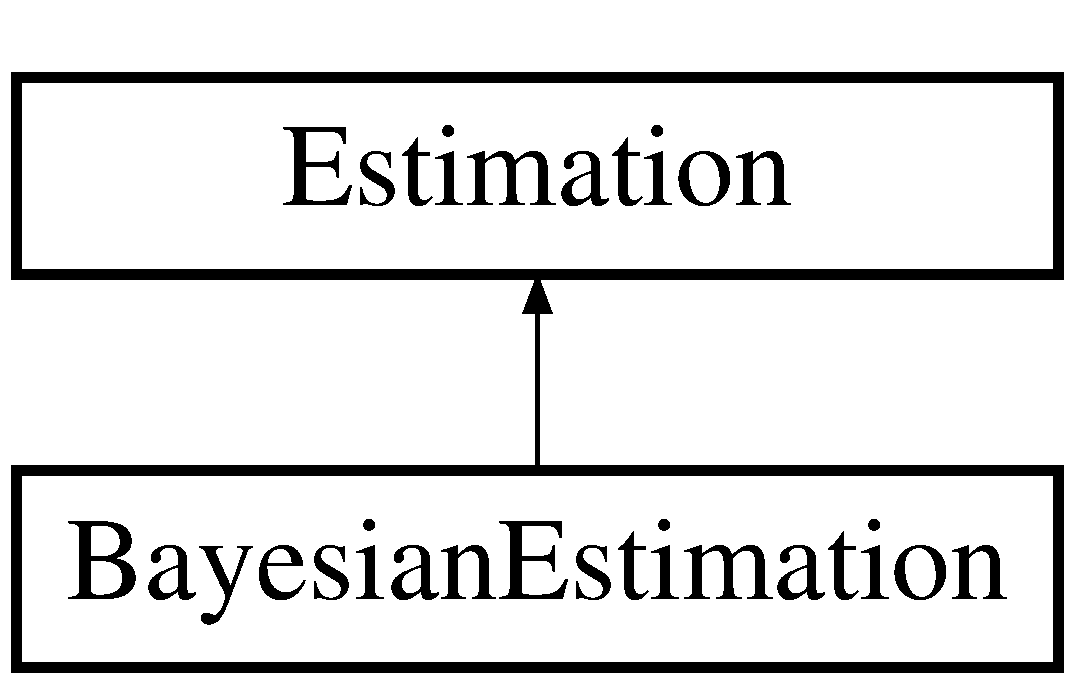
\includegraphics[height=2.000000cm]{classBayesianEstimation}
\end{center}
\end{figure}
\subsection*{Public Member Functions}
\begin{DoxyCompactItemize}
\item 
\hyperlink{classBayesianEstimation_a385093a7d842d5fc1acbb33525b157cf}{Bayesian\+Estimation} ()
\item 
void \hyperlink{classBayesianEstimation_a363ef2a057fe5b20f8724a7ddbb3463b}{estimate} ()
\item 
void \hyperlink{classBayesianEstimation_a46020e91ec07e5e81560fa159a37be16}{set\+Model} (\hyperlink{classModel}{Model} $\ast$)
\item 
virtual \hyperlink{classBayesianEstimation_a8fffb82058cb614a4b20698c24b18cd7}{$\sim$\+Bayesian\+Estimation} ()
\end{DoxyCompactItemize}
\subsection*{Additional Inherited Members}


\subsection{Detailed Description}
\hyperlink{classEstimation}{Estimation} interface for bayesian methods, currently not implemented. 

Definition at line 14 of file Bayesian\+Estimation.\+h.



\subsection{Constructor \& Destructor Documentation}
\hypertarget{classBayesianEstimation_a385093a7d842d5fc1acbb33525b157cf}{}\index{Bayesian\+Estimation@{Bayesian\+Estimation}!Bayesian\+Estimation@{Bayesian\+Estimation}}
\index{Bayesian\+Estimation@{Bayesian\+Estimation}!Bayesian\+Estimation@{Bayesian\+Estimation}}
\subsubsection[{Bayesian\+Estimation}]{\setlength{\rightskip}{0pt plus 5cm}Bayesian\+Estimation\+::\+Bayesian\+Estimation (
\begin{DoxyParamCaption}
{}
\end{DoxyParamCaption}
)}\label{classBayesianEstimation_a385093a7d842d5fc1acbb33525b157cf}


Definition at line 10 of file Bayesian\+Estimation.\+cpp.

\hypertarget{classBayesianEstimation_a8fffb82058cb614a4b20698c24b18cd7}{}\index{Bayesian\+Estimation@{Bayesian\+Estimation}!````~Bayesian\+Estimation@{$\sim$\+Bayesian\+Estimation}}
\index{````~Bayesian\+Estimation@{$\sim$\+Bayesian\+Estimation}!Bayesian\+Estimation@{Bayesian\+Estimation}}
\subsubsection[{$\sim$\+Bayesian\+Estimation}]{\setlength{\rightskip}{0pt plus 5cm}Bayesian\+Estimation\+::$\sim$\+Bayesian\+Estimation (
\begin{DoxyParamCaption}
{}
\end{DoxyParamCaption}
)\hspace{0.3cm}{\ttfamily [virtual]}}\label{classBayesianEstimation_a8fffb82058cb614a4b20698c24b18cd7}


Definition at line 20 of file Bayesian\+Estimation.\+cpp.



\subsection{Member Function Documentation}
\hypertarget{classBayesianEstimation_a363ef2a057fe5b20f8724a7ddbb3463b}{}\index{Bayesian\+Estimation@{Bayesian\+Estimation}!estimate@{estimate}}
\index{estimate@{estimate}!Bayesian\+Estimation@{Bayesian\+Estimation}}
\subsubsection[{estimate}]{\setlength{\rightskip}{0pt plus 5cm}void Bayesian\+Estimation\+::estimate (
\begin{DoxyParamCaption}
{}
\end{DoxyParamCaption}
)\hspace{0.3cm}{\ttfamily [virtual]}}\label{classBayesianEstimation_a363ef2a057fe5b20f8724a7ddbb3463b}


Implements \hyperlink{classEstimation_ab637475bb8ae37f256c94f7b3cdbe848}{Estimation}.



Definition at line 14 of file Bayesian\+Estimation.\+cpp.

\hypertarget{classBayesianEstimation_a46020e91ec07e5e81560fa159a37be16}{}\index{Bayesian\+Estimation@{Bayesian\+Estimation}!set\+Model@{set\+Model}}
\index{set\+Model@{set\+Model}!Bayesian\+Estimation@{Bayesian\+Estimation}}
\subsubsection[{set\+Model}]{\setlength{\rightskip}{0pt plus 5cm}void Bayesian\+Estimation\+::set\+Model (
\begin{DoxyParamCaption}
\item[{{\bf Model} $\ast$}]{model}
\end{DoxyParamCaption}
)\hspace{0.3cm}{\ttfamily [virtual]}}\label{classBayesianEstimation_a46020e91ec07e5e81560fa159a37be16}


Implements \hyperlink{classEstimation_a65f0bd4b60e82a2ab374abd687c69caa}{Estimation}.



Definition at line 17 of file Bayesian\+Estimation.\+cpp.



The documentation for this class was generated from the following files\+:\begin{DoxyCompactItemize}
\item 
src/estimation/bayesian/\hyperlink{BayesianEstimation_8h}{Bayesian\+Estimation.\+h}\item 
src/estimation/bayesian/\hyperlink{BayesianEstimation_8cpp}{Bayesian\+Estimation.\+cpp}\end{DoxyCompactItemize}

\hypertarget{classBlockDiagonalMatrix}{}\section{Block\+Diagonal\+Matrix Class Reference}
\label{classBlockDiagonalMatrix}\index{Block\+Diagonal\+Matrix@{Block\+Diagonal\+Matrix}}


{\ttfamily \#include $<$Block\+Diagonal\+Matrix.\+h$>$}

\subsection*{Public Member Functions}
\begin{DoxyCompactItemize}
\item 
\hyperlink{classBlockDiagonalMatrix_af9a19747fc2d5804b93c395ff7a1cf45}{Block\+Diagonal\+Matrix} ()
\item 
virtual \hyperlink{classBlockDiagonalMatrix_a243790cbfeba5b7b1ddf9bd1ca6e3c73}{$\sim$\+Block\+Diagonal\+Matrix} ()
\end{DoxyCompactItemize}


\subsection{Detailed Description}


Definition at line 11 of file Block\+Diagonal\+Matrix.\+h.



\subsection{Constructor \& Destructor Documentation}
\hypertarget{classBlockDiagonalMatrix_af9a19747fc2d5804b93c395ff7a1cf45}{}\index{Block\+Diagonal\+Matrix@{Block\+Diagonal\+Matrix}!Block\+Diagonal\+Matrix@{Block\+Diagonal\+Matrix}}
\index{Block\+Diagonal\+Matrix@{Block\+Diagonal\+Matrix}!Block\+Diagonal\+Matrix@{Block\+Diagonal\+Matrix}}
\subsubsection[{Block\+Diagonal\+Matrix}]{\setlength{\rightskip}{0pt plus 5cm}Block\+Diagonal\+Matrix\+::\+Block\+Diagonal\+Matrix (
\begin{DoxyParamCaption}
{}
\end{DoxyParamCaption}
)}\label{classBlockDiagonalMatrix_af9a19747fc2d5804b93c395ff7a1cf45}


Definition at line 10 of file Block\+Diagonal\+Matrix.\+cpp.

\hypertarget{classBlockDiagonalMatrix_a243790cbfeba5b7b1ddf9bd1ca6e3c73}{}\index{Block\+Diagonal\+Matrix@{Block\+Diagonal\+Matrix}!````~Block\+Diagonal\+Matrix@{$\sim$\+Block\+Diagonal\+Matrix}}
\index{````~Block\+Diagonal\+Matrix@{$\sim$\+Block\+Diagonal\+Matrix}!Block\+Diagonal\+Matrix@{Block\+Diagonal\+Matrix}}
\subsubsection[{$\sim$\+Block\+Diagonal\+Matrix}]{\setlength{\rightskip}{0pt plus 5cm}Block\+Diagonal\+Matrix\+::$\sim$\+Block\+Diagonal\+Matrix (
\begin{DoxyParamCaption}
{}
\end{DoxyParamCaption}
)\hspace{0.3cm}{\ttfamily [virtual]}}\label{classBlockDiagonalMatrix_a243790cbfeba5b7b1ddf9bd1ca6e3c73}


Definition at line 15 of file Block\+Diagonal\+Matrix.\+cpp.



The documentation for this class was generated from the following files\+:\begin{DoxyCompactItemize}
\item 
src/type/matrix/\hyperlink{BlockDiagonalMatrix_8h}{Block\+Diagonal\+Matrix.\+h}\item 
src/type/matrix/\hyperlink{BlockDiagonalMatrix_8cpp}{Block\+Diagonal\+Matrix.\+cpp}\end{DoxyCompactItemize}

\hypertarget{classClassicalEstimation}{}\section{Classical\+Estimation Class Reference}
\label{classClassicalEstimation}\index{Classical\+Estimation@{Classical\+Estimation}}


Classical estimation class all the classical estimation methods must derive from this class this class is an interface.  




{\ttfamily \#include $<$Classical\+Estimation.\+h$>$}

Inheritance diagram for Classical\+Estimation\+:\begin{figure}[H]
\begin{center}
\leavevmode
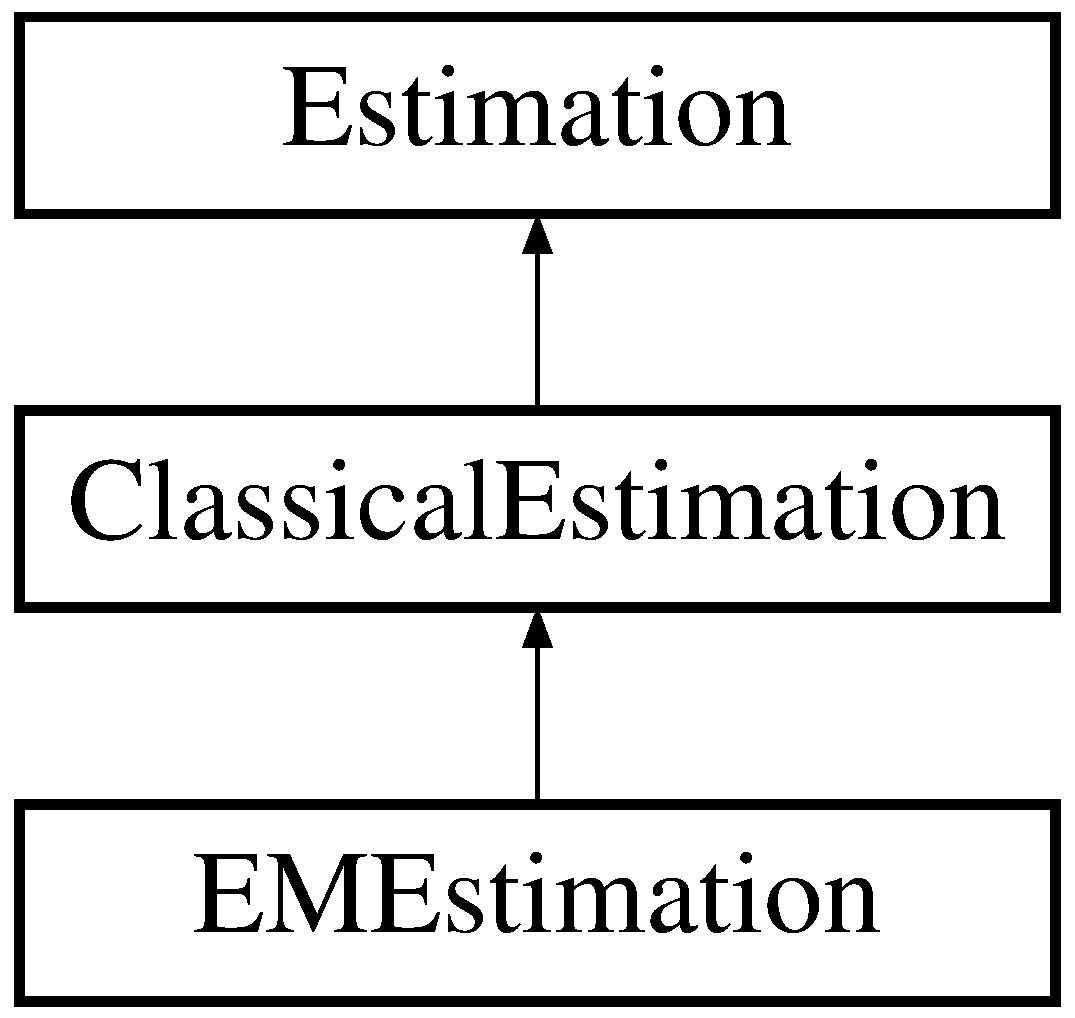
\includegraphics[height=3.000000cm]{classClassicalEstimation}
\end{center}
\end{figure}
\subsection*{Public Member Functions}
\begin{DoxyCompactItemize}
\item 
\hyperlink{classClassicalEstimation_a144021420398e280993eab60a219e1d9}{Classical\+Estimation} ()
\item 
virtual void \hyperlink{classClassicalEstimation_a182aef8049a48cf1bd09bff642df8c01}{estimate} ()=0
\item 
virtual void \hyperlink{classClassicalEstimation_a4add5ad245795b82380af0c34840c603}{set\+Model} (\hyperlink{classModel}{Model} $\ast$)=0
\begin{DoxyCompactList}\small\item\em \hyperlink{classEstimation}{Estimation} method for the item parameters , after executed, the item parameters must be equal to the best parameters for the item according to the model. \end{DoxyCompactList}\item 
virtual \hyperlink{classClassicalEstimation_a6d439cbcdb248008c52a0d59746e3502}{$\sim$\+Classical\+Estimation} ()
\begin{DoxyCompactList}\small\item\em Sets the model for the classical estimation to use. \end{DoxyCompactList}\end{DoxyCompactItemize}
\subsection*{Additional Inherited Members}


\subsection{Detailed Description}
Classical estimation class all the classical estimation methods must derive from this class this class is an interface. 

Definition at line 16 of file Classical\+Estimation.\+h.



\subsection{Constructor \& Destructor Documentation}
\hypertarget{classClassicalEstimation_a144021420398e280993eab60a219e1d9}{}\index{Classical\+Estimation@{Classical\+Estimation}!Classical\+Estimation@{Classical\+Estimation}}
\index{Classical\+Estimation@{Classical\+Estimation}!Classical\+Estimation@{Classical\+Estimation}}
\subsubsection[{Classical\+Estimation}]{\setlength{\rightskip}{0pt plus 5cm}Classical\+Estimation\+::\+Classical\+Estimation (
\begin{DoxyParamCaption}
{}
\end{DoxyParamCaption}
)}\label{classClassicalEstimation_a144021420398e280993eab60a219e1d9}


Definition at line 10 of file Classical\+Estimation.\+cpp.

\hypertarget{classClassicalEstimation_a6d439cbcdb248008c52a0d59746e3502}{}\index{Classical\+Estimation@{Classical\+Estimation}!````~Classical\+Estimation@{$\sim$\+Classical\+Estimation}}
\index{````~Classical\+Estimation@{$\sim$\+Classical\+Estimation}!Classical\+Estimation@{Classical\+Estimation}}
\subsubsection[{$\sim$\+Classical\+Estimation}]{\setlength{\rightskip}{0pt plus 5cm}Classical\+Estimation\+::$\sim$\+Classical\+Estimation (
\begin{DoxyParamCaption}
{}
\end{DoxyParamCaption}
)\hspace{0.3cm}{\ttfamily [virtual]}}\label{classClassicalEstimation_a6d439cbcdb248008c52a0d59746e3502}


Sets the model for the classical estimation to use. 



Definition at line 20 of file Classical\+Estimation.\+cpp.



\subsection{Member Function Documentation}
\hypertarget{classClassicalEstimation_a182aef8049a48cf1bd09bff642df8c01}{}\index{Classical\+Estimation@{Classical\+Estimation}!estimate@{estimate}}
\index{estimate@{estimate}!Classical\+Estimation@{Classical\+Estimation}}
\subsubsection[{estimate}]{\setlength{\rightskip}{0pt plus 5cm}void Classical\+Estimation\+::estimate (
\begin{DoxyParamCaption}
{}
\end{DoxyParamCaption}
)\hspace{0.3cm}{\ttfamily [pure virtual]}}\label{classClassicalEstimation_a182aef8049a48cf1bd09bff642df8c01}


Implements \hyperlink{classEstimation_ab637475bb8ae37f256c94f7b3cdbe848}{Estimation}.



Implemented in \hyperlink{classEMEstimation_a7391808764fd510d6a0f0351ec699b2d}{E\+M\+Estimation}.



Definition at line 14 of file Classical\+Estimation.\+cpp.

\hypertarget{classClassicalEstimation_a4add5ad245795b82380af0c34840c603}{}\index{Classical\+Estimation@{Classical\+Estimation}!set\+Model@{set\+Model}}
\index{set\+Model@{set\+Model}!Classical\+Estimation@{Classical\+Estimation}}
\subsubsection[{set\+Model}]{\setlength{\rightskip}{0pt plus 5cm}void Classical\+Estimation\+::set\+Model (
\begin{DoxyParamCaption}
\item[{{\bf Model} $\ast$}]{model}
\end{DoxyParamCaption}
)\hspace{0.3cm}{\ttfamily [pure virtual]}}\label{classClassicalEstimation_a4add5ad245795b82380af0c34840c603}


\hyperlink{classEstimation}{Estimation} method for the item parameters , after executed, the item parameters must be equal to the best parameters for the item according to the model. 



Implements \hyperlink{classEstimation_a65f0bd4b60e82a2ab374abd687c69caa}{Estimation}.



Implemented in \hyperlink{classEMEstimation_a6cd3ac7193ff9d5d92bd90b58da26e11}{E\+M\+Estimation}.



Definition at line 17 of file Classical\+Estimation.\+cpp.



The documentation for this class was generated from the following files\+:\begin{DoxyCompactItemize}
\item 
src/estimation/classical/\hyperlink{ClassicalEstimation_8h}{Classical\+Estimation.\+h}\item 
src/estimation/classical/\hyperlink{ClassicalEstimation_8cpp}{Classical\+Estimation.\+cpp}\end{DoxyCompactItemize}

\hypertarget{classConstant}{}\section{Constant Class Reference}
\label{classConstant}\index{Constant@{Constant}}


Defines constants used in the S\+I\+C\+S library import this class when using a constant T\+O\+D\+O \+: Config file modification for constants.  




{\ttfamily \#include $<$Constant.\+h$>$}

\subsection*{Static Public Attributes}
\begin{DoxyCompactItemize}
\item 
static double \hyperlink{classConstant_aaf334273fc82a586936f00df7ec30149}{N\+O\+R\+M\+\_\+\+C\+O\+N\+S\+T} = 1
\item 
static double \hyperlink{classConstant_ae5c89860fb1308141f626ba360825f88}{M\+A\+X\+\_\+\+E\+X\+P} = 35.\+0
\item 
static double \hyperlink{classConstant_a37bff4b53634ef172c8d87eded8d29bf}{I\+N\+F\+I\+N\+I\+T\+E} = 1e30
\item 
static double \hyperlink{classConstant_ad5b72f523946f768cdff18907e43155e}{E\+P\+S\+I\+L\+O\+N} = 1e-\/20
\item 
static string \hyperlink{classConstant_ae499a37885b6c873530a91243fd04bdf}{I\+N\+I\+T\+I\+A\+L\+\_\+\+V\+A\+L\+U\+E\+\_\+\+M\+E\+T\+H\+O\+D} = \char`\"{}A\+N\+D\+R\+A\+D\+E\char`\"{}
\item 
static double \hyperlink{classConstant_acc69323a1f124d4b8ed7257e0574a9eb}{stepredn} = 0.\+2
\item 
static double \hyperlink{classConstant_a9fac745f9115a5e2026761c02b5df1d7}{acctol} = 0.\+0001
\item 
static double \hyperlink{classConstant_a3aefd0d2fdfb90049600c25ebcaa41e1}{reltest} = 10.\+0
\item 
static double \hyperlink{classConstant_ae9ad78ce3b1627c1045f78a1045f9d82}{abstol} = 0.\+00001
\item 
static double \hyperlink{classConstant_a46062856afe6595162139069f1157d64}{reltol} = 1e-\/8
\end{DoxyCompactItemize}


\subsection{Detailed Description}
Defines constants used in the S\+I\+C\+S library import this class when using a constant T\+O\+D\+O \+: Config file modification for constants. 

Definition at line 19 of file Constant.\+h.



\subsection{Member Data Documentation}
\hypertarget{classConstant_ae9ad78ce3b1627c1045f78a1045f9d82}{}\index{Constant@{Constant}!abstol@{abstol}}
\index{abstol@{abstol}!Constant@{Constant}}
\subsubsection[{abstol}]{\setlength{\rightskip}{0pt plus 5cm}double Constant\+::abstol = 0.\+00001\hspace{0.3cm}{\ttfamily [static]}}\label{classConstant_ae9ad78ce3b1627c1045f78a1045f9d82}


Definition at line 30 of file Constant.\+h.

\hypertarget{classConstant_a9fac745f9115a5e2026761c02b5df1d7}{}\index{Constant@{Constant}!acctol@{acctol}}
\index{acctol@{acctol}!Constant@{Constant}}
\subsubsection[{acctol}]{\setlength{\rightskip}{0pt plus 5cm}double Constant\+::acctol = 0.\+0001\hspace{0.3cm}{\ttfamily [static]}}\label{classConstant_a9fac745f9115a5e2026761c02b5df1d7}


Definition at line 28 of file Constant.\+h.

\hypertarget{classConstant_ad5b72f523946f768cdff18907e43155e}{}\index{Constant@{Constant}!E\+P\+S\+I\+L\+O\+N@{E\+P\+S\+I\+L\+O\+N}}
\index{E\+P\+S\+I\+L\+O\+N@{E\+P\+S\+I\+L\+O\+N}!Constant@{Constant}}
\subsubsection[{E\+P\+S\+I\+L\+O\+N}]{\setlength{\rightskip}{0pt plus 5cm}double Constant\+::\+E\+P\+S\+I\+L\+O\+N = 1e-\/20\hspace{0.3cm}{\ttfamily [static]}}\label{classConstant_ad5b72f523946f768cdff18907e43155e}


Definition at line 24 of file Constant.\+h.

\hypertarget{classConstant_a37bff4b53634ef172c8d87eded8d29bf}{}\index{Constant@{Constant}!I\+N\+F\+I\+N\+I\+T\+E@{I\+N\+F\+I\+N\+I\+T\+E}}
\index{I\+N\+F\+I\+N\+I\+T\+E@{I\+N\+F\+I\+N\+I\+T\+E}!Constant@{Constant}}
\subsubsection[{I\+N\+F\+I\+N\+I\+T\+E}]{\setlength{\rightskip}{0pt plus 5cm}double Constant\+::\+I\+N\+F\+I\+N\+I\+T\+E = 1e30\hspace{0.3cm}{\ttfamily [static]}}\label{classConstant_a37bff4b53634ef172c8d87eded8d29bf}


Definition at line 23 of file Constant.\+h.

\hypertarget{classConstant_ae499a37885b6c873530a91243fd04bdf}{}\index{Constant@{Constant}!I\+N\+I\+T\+I\+A\+L\+\_\+\+V\+A\+L\+U\+E\+\_\+\+M\+E\+T\+H\+O\+D@{I\+N\+I\+T\+I\+A\+L\+\_\+\+V\+A\+L\+U\+E\+\_\+\+M\+E\+T\+H\+O\+D}}
\index{I\+N\+I\+T\+I\+A\+L\+\_\+\+V\+A\+L\+U\+E\+\_\+\+M\+E\+T\+H\+O\+D@{I\+N\+I\+T\+I\+A\+L\+\_\+\+V\+A\+L\+U\+E\+\_\+\+M\+E\+T\+H\+O\+D}!Constant@{Constant}}
\subsubsection[{I\+N\+I\+T\+I\+A\+L\+\_\+\+V\+A\+L\+U\+E\+\_\+\+M\+E\+T\+H\+O\+D}]{\setlength{\rightskip}{0pt plus 5cm}string Constant\+::\+I\+N\+I\+T\+I\+A\+L\+\_\+\+V\+A\+L\+U\+E\+\_\+\+M\+E\+T\+H\+O\+D = \char`\"{}A\+N\+D\+R\+A\+D\+E\char`\"{}\hspace{0.3cm}{\ttfamily [static]}}\label{classConstant_ae499a37885b6c873530a91243fd04bdf}


Definition at line 25 of file Constant.\+h.

\hypertarget{classConstant_ae5c89860fb1308141f626ba360825f88}{}\index{Constant@{Constant}!M\+A\+X\+\_\+\+E\+X\+P@{M\+A\+X\+\_\+\+E\+X\+P}}
\index{M\+A\+X\+\_\+\+E\+X\+P@{M\+A\+X\+\_\+\+E\+X\+P}!Constant@{Constant}}
\subsubsection[{M\+A\+X\+\_\+\+E\+X\+P}]{\setlength{\rightskip}{0pt plus 5cm}double Constant\+::\+M\+A\+X\+\_\+\+E\+X\+P = 35.\+0\hspace{0.3cm}{\ttfamily [static]}}\label{classConstant_ae5c89860fb1308141f626ba360825f88}


Definition at line 22 of file Constant.\+h.



Referenced by Three\+P\+L\+Model\+::success\+Probability().

\hypertarget{classConstant_aaf334273fc82a586936f00df7ec30149}{}\index{Constant@{Constant}!N\+O\+R\+M\+\_\+\+C\+O\+N\+S\+T@{N\+O\+R\+M\+\_\+\+C\+O\+N\+S\+T}}
\index{N\+O\+R\+M\+\_\+\+C\+O\+N\+S\+T@{N\+O\+R\+M\+\_\+\+C\+O\+N\+S\+T}!Constant@{Constant}}
\subsubsection[{N\+O\+R\+M\+\_\+\+C\+O\+N\+S\+T}]{\setlength{\rightskip}{0pt plus 5cm}double Constant\+::\+N\+O\+R\+M\+\_\+\+C\+O\+N\+S\+T = 1\hspace{0.3cm}{\ttfamily [static]}}\label{classConstant_aaf334273fc82a586936f00df7ec30149}


Definition at line 21 of file Constant.\+h.



Referenced by Three\+P\+L\+Model\+::gradient(), Three\+P\+L\+Model\+::\+Hessian(), and Three\+P\+L\+Model\+::success\+Probability().

\hypertarget{classConstant_a3aefd0d2fdfb90049600c25ebcaa41e1}{}\index{Constant@{Constant}!reltest@{reltest}}
\index{reltest@{reltest}!Constant@{Constant}}
\subsubsection[{reltest}]{\setlength{\rightskip}{0pt plus 5cm}double Constant\+::reltest = 10.\+0\hspace{0.3cm}{\ttfamily [static]}}\label{classConstant_a3aefd0d2fdfb90049600c25ebcaa41e1}


Definition at line 29 of file Constant.\+h.

\hypertarget{classConstant_a46062856afe6595162139069f1157d64}{}\index{Constant@{Constant}!reltol@{reltol}}
\index{reltol@{reltol}!Constant@{Constant}}
\subsubsection[{reltol}]{\setlength{\rightskip}{0pt plus 5cm}double Constant\+::reltol = 1e-\/8\hspace{0.3cm}{\ttfamily [static]}}\label{classConstant_a46062856afe6595162139069f1157d64}


Definition at line 31 of file Constant.\+h.

\hypertarget{classConstant_acc69323a1f124d4b8ed7257e0574a9eb}{}\index{Constant@{Constant}!stepredn@{stepredn}}
\index{stepredn@{stepredn}!Constant@{Constant}}
\subsubsection[{stepredn}]{\setlength{\rightskip}{0pt plus 5cm}double Constant\+::stepredn = 0.\+2\hspace{0.3cm}{\ttfamily [static]}}\label{classConstant_acc69323a1f124d4b8ed7257e0574a9eb}


Definition at line 27 of file Constant.\+h.



The documentation for this class was generated from the following files\+:\begin{DoxyCompactItemize}
\item 
src/type/\hyperlink{Constant_8h}{Constant.\+h}\item 
src/type/\hyperlink{Constant_8cpp}{Constant.\+cpp}\end{DoxyCompactItemize}

\hypertarget{classDataSet}{}\section{Data\+Set Class Reference}
\label{classDataSet}\index{Data\+Set@{Data\+Set}}


Skeleton class for the datasets a dataset can contain not only the raw matrices but information about the dataset.  




{\ttfamily \#include $<$Data\+Set.\+h$>$}

Inheritance diagram for Data\+Set\+:\begin{figure}[H]
\begin{center}
\leavevmode
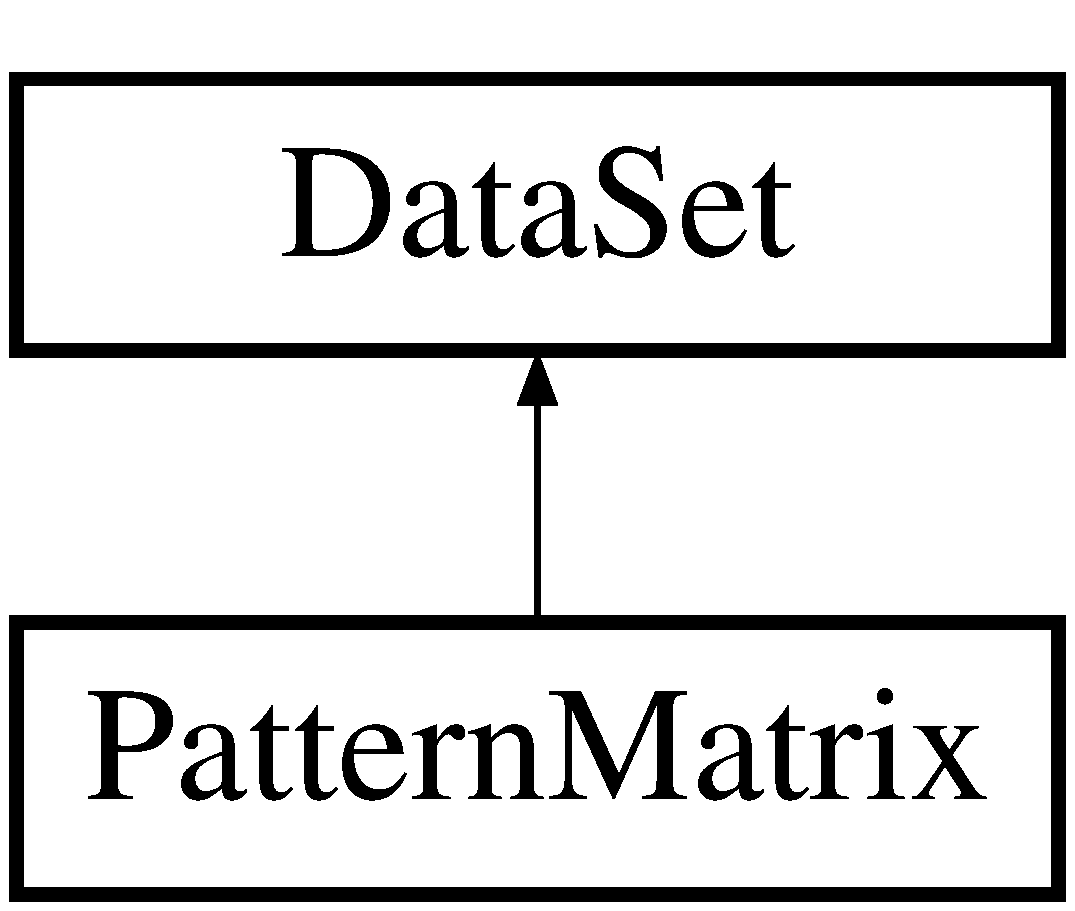
\includegraphics[height=2.000000cm]{classDataSet}
\end{center}
\end{figure}
\subsection*{Public Member Functions}
\begin{DoxyCompactItemize}
\item 
virtual int \hyperlink{classDataSet_acbd07a4d4acc27332ec4f323e600885a}{count\+Items} () const =0
\item 
virtual int \hyperlink{classDataSet_a0514da0d8d87fc9503458b3c11978e67}{count\+Individuals} () const =0
\item 
virtual \hyperlink{classDataSet_a2cdb84d32331956b413ca36933e516bd}{$\sim$\+Data\+Set} ()
\end{DoxyCompactItemize}


\subsection{Detailed Description}
Skeleton class for the datasets a dataset can contain not only the raw matrices but information about the dataset. 

Definition at line 16 of file Data\+Set.\+h.



\subsection{Constructor \& Destructor Documentation}
\hypertarget{classDataSet_a2cdb84d32331956b413ca36933e516bd}{}\index{Data\+Set@{Data\+Set}!````~Data\+Set@{$\sim$\+Data\+Set}}
\index{````~Data\+Set@{$\sim$\+Data\+Set}!Data\+Set@{Data\+Set}}
\subsubsection[{$\sim$\+Data\+Set}]{\setlength{\rightskip}{0pt plus 5cm}Data\+Set\+::$\sim$\+Data\+Set (
\begin{DoxyParamCaption}
{}
\end{DoxyParamCaption}
)\hspace{0.3cm}{\ttfamily [virtual]}}\label{classDataSet_a2cdb84d32331956b413ca36933e516bd}


Definition at line 10 of file Data\+Set.\+cpp.



\subsection{Member Function Documentation}
\hypertarget{classDataSet_a0514da0d8d87fc9503458b3c11978e67}{}\index{Data\+Set@{Data\+Set}!count\+Individuals@{count\+Individuals}}
\index{count\+Individuals@{count\+Individuals}!Data\+Set@{Data\+Set}}
\subsubsection[{count\+Individuals}]{\setlength{\rightskip}{0pt plus 5cm}virtual int Data\+Set\+::count\+Individuals (
\begin{DoxyParamCaption}
{}
\end{DoxyParamCaption}
) const\hspace{0.3cm}{\ttfamily [pure virtual]}}\label{classDataSet_a0514da0d8d87fc9503458b3c11978e67}


Implemented in \hyperlink{classPatternMatrix_afd88d101ed9a74ed78c94e3eb024e448}{Pattern\+Matrix}.

\hypertarget{classDataSet_acbd07a4d4acc27332ec4f323e600885a}{}\index{Data\+Set@{Data\+Set}!count\+Items@{count\+Items}}
\index{count\+Items@{count\+Items}!Data\+Set@{Data\+Set}}
\subsubsection[{count\+Items}]{\setlength{\rightskip}{0pt plus 5cm}virtual int Data\+Set\+::count\+Items (
\begin{DoxyParamCaption}
{}
\end{DoxyParamCaption}
) const\hspace{0.3cm}{\ttfamily [pure virtual]}}\label{classDataSet_acbd07a4d4acc27332ec4f323e600885a}


Implemented in \hyperlink{classPatternMatrix_adaa3ade657d4ed832a359be5954d842b}{Pattern\+Matrix}.



Referenced by E\+M\+Estimation\+::step\+M().



The documentation for this class was generated from the following files\+:\begin{DoxyCompactItemize}
\item 
src/type/\hyperlink{DataSet_8h}{Data\+Set.\+h}\item 
src/type/\hyperlink{DataSet_8cpp}{Data\+Set.\+cpp}\end{DoxyCompactItemize}

\hypertarget{classDichotomousModel}{}\section{Dichotomous\+Model Class Reference}
\label{classDichotomousModel}\index{Dichotomous\+Model@{Dichotomous\+Model}}


{\ttfamily \#include $<$Dichotomous\+Model.\+h$>$}

Inheritance diagram for Dichotomous\+Model\+:\begin{figure}[H]
\begin{center}
\leavevmode
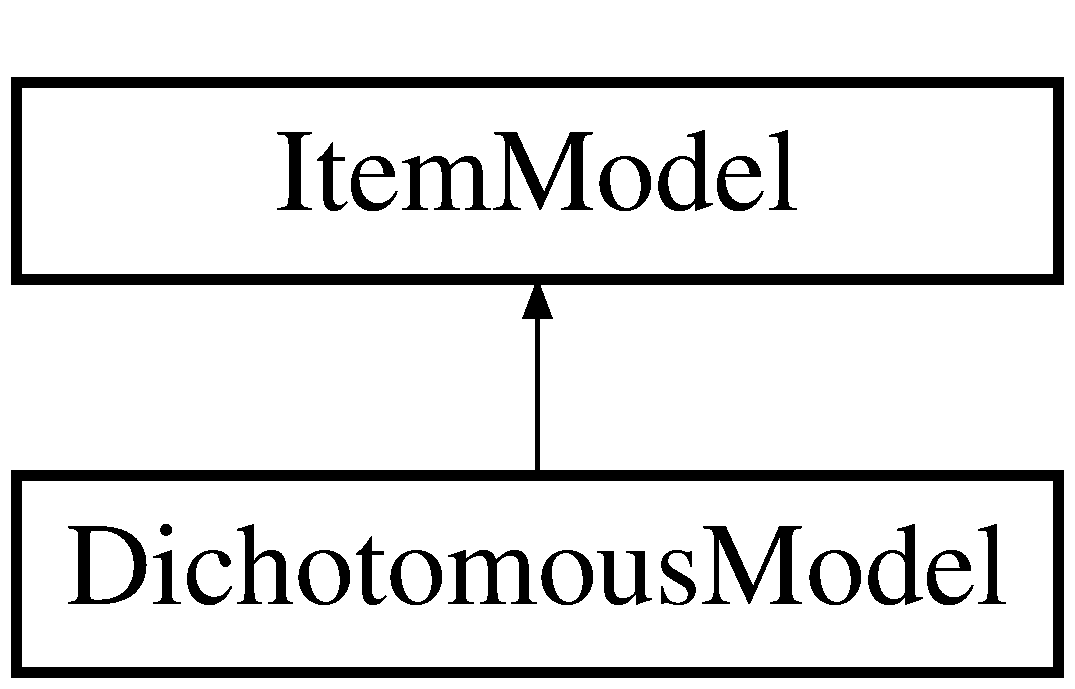
\includegraphics[height=2.000000cm]{classDichotomousModel}
\end{center}
\end{figure}
\subsection*{Public Member Functions}
\begin{DoxyCompactItemize}
\item 
\hyperlink{classDichotomousModel_a0938ae1266fcd8d72e78b14c55e5e214}{Dichotomous\+Model} ()
\item 
int \hyperlink{classDichotomousModel_a6861f3ef96b4525ba1b1db1a7dfb1ca3}{count\+Categories} ()
\item 
int \hyperlink{classDichotomousModel_ae9dfca33b3549ea73e4fc8fcab204cc0}{count\+Items} ()
\item 
\hyperlink{classDataSet}{Data\+Set} $\ast$ \hyperlink{classDichotomousModel_a0fd6d3ed3a6e78f7a65caa9d2828c7c6}{get\+Dataset} ()
\item 
void \hyperlink{classDichotomousModel_a5e7bf92bc598e581477b9c5814ca7f72}{set\+Dataset} (\hyperlink{classDataSet}{Data\+Set} $\ast$dataset)
\item 
virtual \hyperlink{classDichotomousModel_ae7500fc776e29cad3f2a6675f83ae22f}{$\sim$\+Dichotomous\+Model} ()
\end{DoxyCompactItemize}
\subsection*{Additional Inherited Members}


\subsection{Detailed Description}


Definition at line 14 of file Dichotomous\+Model.\+h.



\subsection{Constructor \& Destructor Documentation}
\hypertarget{classDichotomousModel_a0938ae1266fcd8d72e78b14c55e5e214}{}\index{Dichotomous\+Model@{Dichotomous\+Model}!Dichotomous\+Model@{Dichotomous\+Model}}
\index{Dichotomous\+Model@{Dichotomous\+Model}!Dichotomous\+Model@{Dichotomous\+Model}}
\subsubsection[{Dichotomous\+Model}]{\setlength{\rightskip}{0pt plus 5cm}Dichotomous\+Model\+::\+Dichotomous\+Model (
\begin{DoxyParamCaption}
{}
\end{DoxyParamCaption}
)}\label{classDichotomousModel_a0938ae1266fcd8d72e78b14c55e5e214}


Definition at line 10 of file Dichotomous\+Model.\+cpp.

\hypertarget{classDichotomousModel_ae7500fc776e29cad3f2a6675f83ae22f}{}\index{Dichotomous\+Model@{Dichotomous\+Model}!````~Dichotomous\+Model@{$\sim$\+Dichotomous\+Model}}
\index{````~Dichotomous\+Model@{$\sim$\+Dichotomous\+Model}!Dichotomous\+Model@{Dichotomous\+Model}}
\subsubsection[{$\sim$\+Dichotomous\+Model}]{\setlength{\rightskip}{0pt plus 5cm}Dichotomous\+Model\+::$\sim$\+Dichotomous\+Model (
\begin{DoxyParamCaption}
{}
\end{DoxyParamCaption}
)\hspace{0.3cm}{\ttfamily [virtual]}}\label{classDichotomousModel_ae7500fc776e29cad3f2a6675f83ae22f}


Definition at line 32 of file Dichotomous\+Model.\+cpp.



\subsection{Member Function Documentation}
\hypertarget{classDichotomousModel_a6861f3ef96b4525ba1b1db1a7dfb1ca3}{}\index{Dichotomous\+Model@{Dichotomous\+Model}!count\+Categories@{count\+Categories}}
\index{count\+Categories@{count\+Categories}!Dichotomous\+Model@{Dichotomous\+Model}}
\subsubsection[{count\+Categories}]{\setlength{\rightskip}{0pt plus 5cm}int Dichotomous\+Model\+::count\+Categories (
\begin{DoxyParamCaption}
{}
\end{DoxyParamCaption}
)\hspace{0.3cm}{\ttfamily [virtual]}}\label{classDichotomousModel_a6861f3ef96b4525ba1b1db1a7dfb1ca3}


Implements \hyperlink{classItemModel_af0aabe9f48c6d111fbcb903cb330fae7}{Item\+Model}.



Definition at line 15 of file Dichotomous\+Model.\+cpp.

\hypertarget{classDichotomousModel_ae9dfca33b3549ea73e4fc8fcab204cc0}{}\index{Dichotomous\+Model@{Dichotomous\+Model}!count\+Items@{count\+Items}}
\index{count\+Items@{count\+Items}!Dichotomous\+Model@{Dichotomous\+Model}}
\subsubsection[{count\+Items}]{\setlength{\rightskip}{0pt plus 5cm}int Dichotomous\+Model\+::count\+Items (
\begin{DoxyParamCaption}
{}
\end{DoxyParamCaption}
)\hspace{0.3cm}{\ttfamily [virtual]}}\label{classDichotomousModel_ae9dfca33b3549ea73e4fc8fcab204cc0}


Implements \hyperlink{classItemModel_a7a93c60e346f4d80f265a4c9e083181d}{Item\+Model}.



Definition at line 27 of file Dichotomous\+Model.\+cpp.



References Pattern\+Matrix\+::count\+Items(), and Item\+Model\+::data\+Set.

\hypertarget{classDichotomousModel_a0fd6d3ed3a6e78f7a65caa9d2828c7c6}{}\index{Dichotomous\+Model@{Dichotomous\+Model}!get\+Dataset@{get\+Dataset}}
\index{get\+Dataset@{get\+Dataset}!Dichotomous\+Model@{Dichotomous\+Model}}
\subsubsection[{get\+Dataset}]{\setlength{\rightskip}{0pt plus 5cm}{\bf Data\+Set} $\ast$ Dichotomous\+Model\+::get\+Dataset (
\begin{DoxyParamCaption}
{}
\end{DoxyParamCaption}
)\hspace{0.3cm}{\ttfamily [virtual]}}\label{classDichotomousModel_a0fd6d3ed3a6e78f7a65caa9d2828c7c6}


Implements \hyperlink{classItemModel_a8521ea3f8f511e88d5257ff7591cd928}{Item\+Model}.



Definition at line 19 of file Dichotomous\+Model.\+cpp.



References Item\+Model\+::data\+Set.

\hypertarget{classDichotomousModel_a5e7bf92bc598e581477b9c5814ca7f72}{}\index{Dichotomous\+Model@{Dichotomous\+Model}!set\+Dataset@{set\+Dataset}}
\index{set\+Dataset@{set\+Dataset}!Dichotomous\+Model@{Dichotomous\+Model}}
\subsubsection[{set\+Dataset}]{\setlength{\rightskip}{0pt plus 5cm}void Dichotomous\+Model\+::set\+Dataset (
\begin{DoxyParamCaption}
\item[{{\bf Data\+Set} $\ast$}]{dataset}
\end{DoxyParamCaption}
)\hspace{0.3cm}{\ttfamily [virtual]}}\label{classDichotomousModel_a5e7bf92bc598e581477b9c5814ca7f72}


Implements \hyperlink{classItemModel_accd6c6b6827c45970d04c22baaca6b0c}{Item\+Model}.



Definition at line 23 of file Dichotomous\+Model.\+cpp.



References Item\+Model\+::data\+Set.



The documentation for this class was generated from the following files\+:\begin{DoxyCompactItemize}
\item 
src/model/item/\hyperlink{DichotomousModel_8h}{Dichotomous\+Model.\+h}\item 
src/model/item/\hyperlink{DichotomousModel_8cpp}{Dichotomous\+Model.\+cpp}\end{DoxyCompactItemize}

\hypertarget{classDimensionModel}{}\section{Dimension\+Model Class Reference}
\label{classDimensionModel}\index{Dimension\+Model@{Dimension\+Model}}


{\ttfamily \#include $<$Dimension\+Model.\+h$>$}

Inheritance diagram for Dimension\+Model\+:\begin{figure}[H]
\begin{center}
\leavevmode
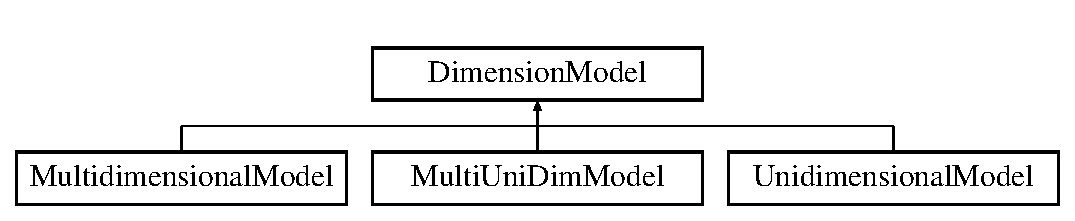
\includegraphics[height=2.000000cm]{classDimensionModel}
\end{center}
\end{figure}
\subsection*{Public Member Functions}
\begin{DoxyCompactItemize}
\item 
virtual int \hyperlink{classDimensionModel_aaf16c9215f4a7d08d67bd844adfcc62a}{get\+Num\+Dimensions} ()=0
\item 
virtual vector$<$ int $>$ \hyperlink{classDimensionModel_a0aab2664f71949ac52d654730840056b}{get\+Dim\+Vector} ()=0
\item 
virtual \hyperlink{classLatentTraitSet}{Latent\+Trait\+Set} $\ast$ \hyperlink{classDimensionModel_a37d2d9ab998a4e65628571e6144311f6}{get\+Latent\+Trait\+Set} () const =0
\item 
virtual void \hyperlink{classDimensionModel_aed42259f6cd663cbd1df07d18d4b1e07}{set\+Latent\+Trait\+Set} (\hyperlink{classLatentTraitSet}{Latent\+Trait\+Set} $\ast$\hyperlink{classDimensionModel_af202cd5a44ee99d865674c6e26d770c8}{latent\+Trait\+Set})=0
\item 
virtual \hyperlink{classDimensionModel_aa7bb6d6c4ef9cab805d02a66778be361}{$\sim$\+Dimension\+Model} ()
\end{DoxyCompactItemize}
\subsection*{Protected Attributes}
\begin{DoxyCompactItemize}
\item 
\hyperlink{classLatentTraitSet}{Latent\+Trait\+Set} $\ast$ \hyperlink{classDimensionModel_af202cd5a44ee99d865674c6e26d770c8}{latent\+Trait\+Set}
\end{DoxyCompactItemize}


\subsection{Detailed Description}


Definition at line 16 of file Dimension\+Model.\+h.



\subsection{Constructor \& Destructor Documentation}
\hypertarget{classDimensionModel_aa7bb6d6c4ef9cab805d02a66778be361}{}\index{Dimension\+Model@{Dimension\+Model}!````~Dimension\+Model@{$\sim$\+Dimension\+Model}}
\index{````~Dimension\+Model@{$\sim$\+Dimension\+Model}!Dimension\+Model@{Dimension\+Model}}
\subsubsection[{$\sim$\+Dimension\+Model}]{\setlength{\rightskip}{0pt plus 5cm}Dimension\+Model\+::$\sim$\+Dimension\+Model (
\begin{DoxyParamCaption}
{}
\end{DoxyParamCaption}
)\hspace{0.3cm}{\ttfamily [virtual]}}\label{classDimensionModel_aa7bb6d6c4ef9cab805d02a66778be361}


Definition at line 10 of file Dimension\+Model.\+cpp.



\subsection{Member Function Documentation}
\hypertarget{classDimensionModel_a0aab2664f71949ac52d654730840056b}{}\index{Dimension\+Model@{Dimension\+Model}!get\+Dim\+Vector@{get\+Dim\+Vector}}
\index{get\+Dim\+Vector@{get\+Dim\+Vector}!Dimension\+Model@{Dimension\+Model}}
\subsubsection[{get\+Dim\+Vector}]{\setlength{\rightskip}{0pt plus 5cm}virtual vector$<$int$>$ Dimension\+Model\+::get\+Dim\+Vector (
\begin{DoxyParamCaption}
{}
\end{DoxyParamCaption}
)\hspace{0.3cm}{\ttfamily [pure virtual]}}\label{classDimensionModel_a0aab2664f71949ac52d654730840056b}


Implemented in \hyperlink{classMultidimensionalModel_a6834137ae4a9d43cd73cf31025258059}{Multidimensional\+Model}, \hyperlink{classMultiUniDimModel_a1e92f67a87f5b406f0382e9cb240f889}{Multi\+Uni\+Dim\+Model}, and \hyperlink{classUnidimensionalModel_a31d345c00b118a0c9efdc36592d4edd1}{Unidimensional\+Model}.

\hypertarget{classDimensionModel_a37d2d9ab998a4e65628571e6144311f6}{}\index{Dimension\+Model@{Dimension\+Model}!get\+Latent\+Trait\+Set@{get\+Latent\+Trait\+Set}}
\index{get\+Latent\+Trait\+Set@{get\+Latent\+Trait\+Set}!Dimension\+Model@{Dimension\+Model}}
\subsubsection[{get\+Latent\+Trait\+Set}]{\setlength{\rightskip}{0pt plus 5cm}virtual {\bf Latent\+Trait\+Set}$\ast$ Dimension\+Model\+::get\+Latent\+Trait\+Set (
\begin{DoxyParamCaption}
{}
\end{DoxyParamCaption}
) const\hspace{0.3cm}{\ttfamily [pure virtual]}}\label{classDimensionModel_a37d2d9ab998a4e65628571e6144311f6}


Implemented in \hyperlink{classMultidimensionalModel_a94d8dcb1f23f8fa8223ef7cc2d7f860d}{Multidimensional\+Model}, \hyperlink{classMultiUniDimModel_aa3b9917e93a9498f5eb95c74a2335797}{Multi\+Uni\+Dim\+Model}, and \hyperlink{classUnidimensionalModel_a1876249eafaaa89b145c50adc8b4745a}{Unidimensional\+Model}.



Referenced by Three\+P\+L\+Model\+::build\+Parameter\+Set(), one\+Run(), E\+M\+Estimation\+::set\+Model(), E\+M\+Estimation\+::step\+E(), E\+M\+Estimation\+::step\+M(), and Three\+P\+L\+Model\+::success\+Probability().

\hypertarget{classDimensionModel_aaf16c9215f4a7d08d67bd844adfcc62a}{}\index{Dimension\+Model@{Dimension\+Model}!get\+Num\+Dimensions@{get\+Num\+Dimensions}}
\index{get\+Num\+Dimensions@{get\+Num\+Dimensions}!Dimension\+Model@{Dimension\+Model}}
\subsubsection[{get\+Num\+Dimensions}]{\setlength{\rightskip}{0pt plus 5cm}virtual int Dimension\+Model\+::get\+Num\+Dimensions (
\begin{DoxyParamCaption}
{}
\end{DoxyParamCaption}
)\hspace{0.3cm}{\ttfamily [pure virtual]}}\label{classDimensionModel_aaf16c9215f4a7d08d67bd844adfcc62a}


Implemented in \hyperlink{classMultidimensionalModel_ad76fe466abfab3c05bb86519440d0302}{Multidimensional\+Model}, \hyperlink{classMultiUniDimModel_a6789b80610d6db4985dc51020313b158}{Multi\+Uni\+Dim\+Model}, and \hyperlink{classUnidimensionalModel_a98a0a8d59c3b7d770579dba0a14f4802}{Unidimensional\+Model}.

\hypertarget{classDimensionModel_aed42259f6cd663cbd1df07d18d4b1e07}{}\index{Dimension\+Model@{Dimension\+Model}!set\+Latent\+Trait\+Set@{set\+Latent\+Trait\+Set}}
\index{set\+Latent\+Trait\+Set@{set\+Latent\+Trait\+Set}!Dimension\+Model@{Dimension\+Model}}
\subsubsection[{set\+Latent\+Trait\+Set}]{\setlength{\rightskip}{0pt plus 5cm}virtual void Dimension\+Model\+::set\+Latent\+Trait\+Set (
\begin{DoxyParamCaption}
\item[{{\bf Latent\+Trait\+Set} $\ast$}]{latent\+Trait\+Set}
\end{DoxyParamCaption}
)\hspace{0.3cm}{\ttfamily [pure virtual]}}\label{classDimensionModel_aed42259f6cd663cbd1df07d18d4b1e07}


Implemented in \hyperlink{classMultidimensionalModel_a367cc1d66122b0f56293271a0ffd4859}{Multidimensional\+Model}, \hyperlink{classMultiUniDimModel_ac13d9476e8687888d1a290704561e704}{Multi\+Uni\+Dim\+Model}, and \hyperlink{classUnidimensionalModel_ab71959d21ff63f9d2fc15cf6a815b408}{Unidimensional\+Model}.



\subsection{Member Data Documentation}
\hypertarget{classDimensionModel_af202cd5a44ee99d865674c6e26d770c8}{}\index{Dimension\+Model@{Dimension\+Model}!latent\+Trait\+Set@{latent\+Trait\+Set}}
\index{latent\+Trait\+Set@{latent\+Trait\+Set}!Dimension\+Model@{Dimension\+Model}}
\subsubsection[{latent\+Trait\+Set}]{\setlength{\rightskip}{0pt plus 5cm}{\bf Latent\+Trait\+Set}$\ast$ Dimension\+Model\+::latent\+Trait\+Set\hspace{0.3cm}{\ttfamily [protected]}}\label{classDimensionModel_af202cd5a44ee99d865674c6e26d770c8}


Definition at line 18 of file Dimension\+Model.\+h.



Referenced by Unidimensional\+Model\+::get\+Dim\+Vector(), Multi\+Uni\+Dim\+Model\+::get\+Latent\+Trait\+Set(), Unidimensional\+Model\+::get\+Latent\+Trait\+Set(), Multidimensional\+Model\+::get\+Latent\+Trait\+Set(), Multi\+Uni\+Dim\+Model\+::set\+Latent\+Trait\+Set(), Unidimensional\+Model\+::set\+Latent\+Trait\+Set(), Multidimensional\+Model\+::set\+Latent\+Trait\+Set(), Unidimensional\+Model\+::\+Unidimensional\+Model(), and Unidimensional\+Model\+::$\sim$\+Unidimensional\+Model().



The documentation for this class was generated from the following files\+:\begin{DoxyCompactItemize}
\item 
src/model/dimension/\hyperlink{DimensionModel_8h}{Dimension\+Model.\+h}\item 
src/model/dimension/\hyperlink{DimensionModel_8cpp}{Dimension\+Model.\+cpp}\end{DoxyCompactItemize}

\hypertarget{classEMEstimation}{}\section{E\+M\+Estimation Class Reference}
\label{classEMEstimation}\index{E\+M\+Estimation@{E\+M\+Estimation}}


Classical estimation through the E\+M algorithm, generic for the models however must be called with specific model object, the optimization algorithm can be any from the optimizers class.  




{\ttfamily \#include $<$E\+M\+Estimation.\+h$>$}

Inheritance diagram for E\+M\+Estimation\+:\begin{figure}[H]
\begin{center}
\leavevmode
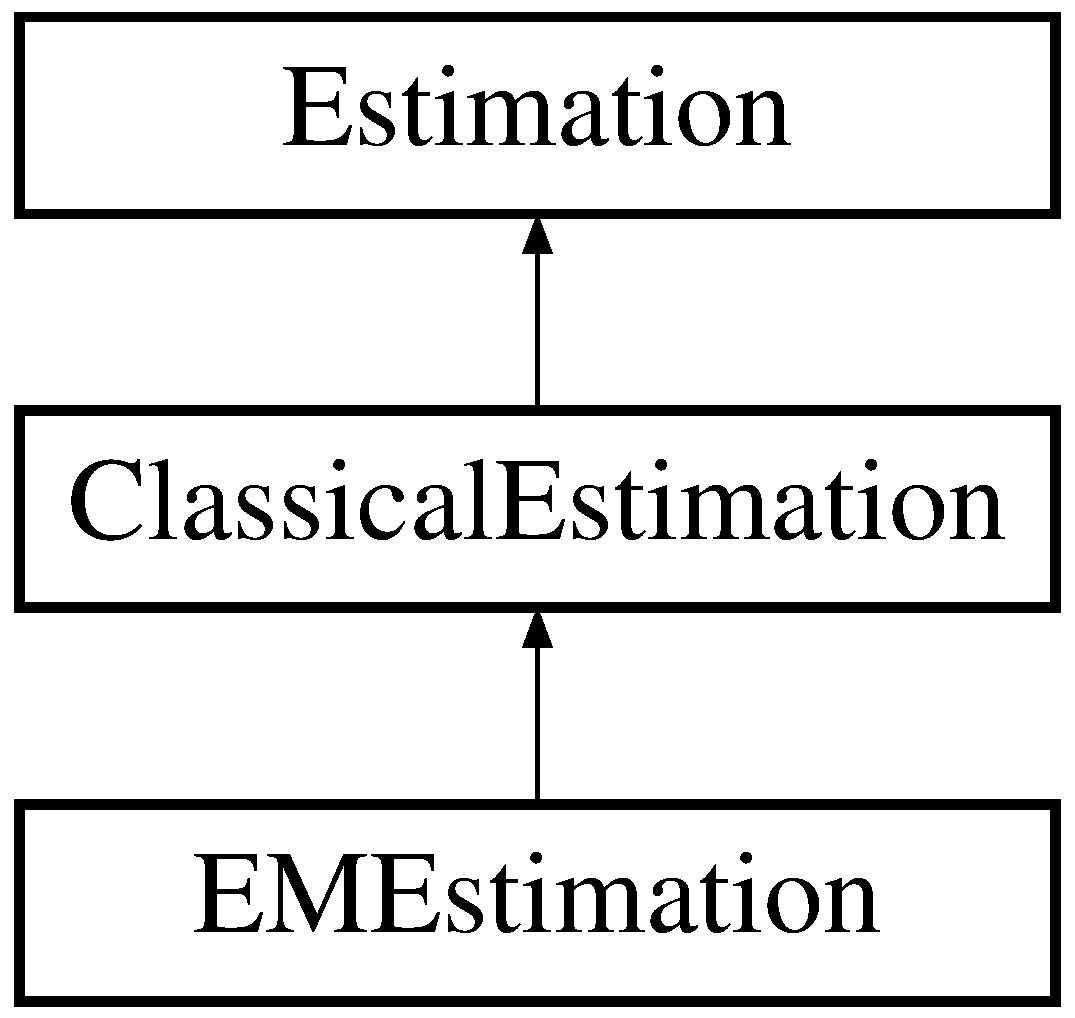
\includegraphics[height=3.000000cm]{classEMEstimation}
\end{center}
\end{figure}
\subsection*{Public Member Functions}
\begin{DoxyCompactItemize}
\item 
\hyperlink{classEMEstimation_a942acb2a0dcbd99dbd2669d6743e0e51}{E\+M\+Estimation} ()
\item 
virtual \hyperlink{classEMEstimation_a218c478d8b1b49c4ea9076ba30852c9d}{$\sim$\+E\+M\+Estimation} ()
\item 
void \hyperlink{classEMEstimation_a7391808764fd510d6a0f0351ec699b2d}{estimate} ()
\begin{DoxyCompactList}\small\item\em Main loop of the E\+M estimation orchestrates the parameters for the estimation, and holds the estimation for the iterations. \end{DoxyCompactList}\item 
void \hyperlink{classEMEstimation_afd00a80808f85581961d4d0ed2ce2a97}{step\+E} ()
\begin{DoxyCompactList}\small\item\em Step E of the E\+M method, this step takes the actual estimation of the parameters, and produces a f and a r matrices used in the maximization step. \end{DoxyCompactList}\item 
void \hyperlink{classEMEstimation_a8884e863f820e4a1a5caf099dca2ce1b}{step\+M} ()
\begin{DoxyCompactList}\small\item\em Executes the maximization step using the inputted or default optimizer currently only supporting B\+F\+G\+S and newton algorithms. \end{DoxyCompactList}\item 
void \hyperlink{classEMEstimation_a6cd3ac7193ff9d5d92bd90b58da26e11}{set\+Model} (\hyperlink{classModel}{Model} $\ast$\hyperlink{classEMEstimation_ad7a5d7459c7c0632a1aa3917fd7f3ba0}{model})
\begin{DoxyCompactList}\small\item\em Sets the model to be estimated, currently only supports 3\+P\+L model. \end{DoxyCompactList}\item 
void \hyperlink{classEMEstimation_a482fdb64918b8e5d68e2f5091bef4b05}{check\+Running\+Conditions} ()
\begin{DoxyCompactList}\small\item\em Check if all the conditions are met for running the model, can report an error to a logger. \end{DoxyCompactList}\item 
void \hyperlink{classEMEstimation_aa599b89650be2a1f95c1a986af5755f2}{set\+Optimization\+Algorithm} (string algorithm)
\begin{DoxyCompactList}\small\item\em Sets the optimization algorithm. \end{DoxyCompactList}\item 
void \hyperlink{classEMEstimation_ae8d8d6a4f2874d0da59ae2f57f21750a}{set\+Trace} (string filename)
\begin{DoxyCompactList}\small\item\em Sets the reporter for the trace. \end{DoxyCompactList}\item 
void \hyperlink{classEMEstimation_aadb720a89ed634dff963c4d50970b249}{set\+Trace} (\hyperlink{classTrace}{Trace} trace)
\item 
void \hyperlink{classEMEstimation_a1f773c655ba098b5d6c8269de00003c3}{set\+Initial\+Values} (map$<$ \hyperlink{ParameterModel_8h_a04ed5b8f1f3adf7af1d5092fae847e90}{Parameter}, \hyperlink{singletonMatrix}{Matrix}$<$ double $>$ $\ast$ $>$ parameter\+Set)
\begin{DoxyCompactList}\small\item\em Sets the initial values for the estimation, use this for inputting a matrix as initial values. \end{DoxyCompactList}\item 
void \hyperlink{classEMEstimation_a9e6a83bfa5f78ec1531f67538dc12f93}{set\+Initial\+Values} (string method)
\begin{DoxyCompactList}\small\item\em Sets the initial values according to a method of calculating the values Possible methods \+: A\+N\+D\+R\+A\+D\+E, O\+S\+P\+I\+N\+A, R\+A\+N\+D\+O\+M,. \end{DoxyCompactList}\item 
int \hyperlink{classEMEstimation_a939385baead6848507efd5949906f50b}{get\+Iterations} () const 
\begin{DoxyCompactList}\small\item\em Returns the iterations that took the estimation to obtain an answer. \end{DoxyCompactList}\end{DoxyCompactItemize}
\subsection*{Private Attributes}
\begin{DoxyCompactItemize}
\item 
\hyperlink{singletonMatrix}{Matrix}$<$ double $>$ $\ast$ \hyperlink{classEMEstimation_a4ad566123ad607b791d56990f9dd096d}{f}
\item 
\hyperlink{singletonMatrix}{Matrix}$<$ double $>$ $\ast$ \hyperlink{classEMEstimation_a426db380391c487206521631156d7eb6}{r}
\item 
\hyperlink{classTrace}{Trace} $\ast$ \hyperlink{classEMEstimation_a77ab33231a9baa8c5a2ceb48534137a0}{logger}
\item 
\hyperlink{classModel}{Model} $\ast$ \hyperlink{classEMEstimation_ad7a5d7459c7c0632a1aa3917fd7f3ba0}{model}
\item 
\hyperlink{classOptimizer}{Optimizer} $\ast$ \hyperlink{classEMEstimation_abbabf603bb09b6338114dd53aef5bd8a}{optim}
\item 
bool \hyperlink{classEMEstimation_aaa1a979767c171c5d33ee1ac77838ac2}{convergence\+Signal}
\item 
int \hyperlink{classEMEstimation_ad6086e6784a5c651e6d5ad45a0c84d11}{iterations}
\end{DoxyCompactItemize}
\subsection*{Additional Inherited Members}


\subsection{Detailed Description}
Classical estimation through the E\+M algorithm, generic for the models however must be called with specific model object, the optimization algorithm can be any from the optimizers class. 

E\+M is a iterative \hyperlink{classEstimation}{Estimation} Maximization algorithm, please check the literature on how it works. E\+M estimation requires a quadrature for the implementation of the integrals in the expectation step this quadratures can be obtained from R, or using the supplied ones from the S\+I\+C\+S binary quadratures ranging from 1 quadrature node to 101 quadrature nodes. 

Definition at line 25 of file E\+M\+Estimation.\+h.



\subsection{Constructor \& Destructor Documentation}
\hypertarget{classEMEstimation_a942acb2a0dcbd99dbd2669d6743e0e51}{}\index{E\+M\+Estimation@{E\+M\+Estimation}!E\+M\+Estimation@{E\+M\+Estimation}}
\index{E\+M\+Estimation@{E\+M\+Estimation}!E\+M\+Estimation@{E\+M\+Estimation}}
\subsubsection[{E\+M\+Estimation}]{\setlength{\rightskip}{0pt plus 5cm}E\+M\+Estimation\+::\+E\+M\+Estimation (
\begin{DoxyParamCaption}
{}
\end{DoxyParamCaption}
)}\label{classEMEstimation_a942acb2a0dcbd99dbd2669d6743e0e51}


Definition at line 11 of file E\+M\+Estimation.\+cpp.



References convergence\+Signal, f, iterations, logger, model, optim, and r.

\hypertarget{classEMEstimation_a218c478d8b1b49c4ea9076ba30852c9d}{}\index{E\+M\+Estimation@{E\+M\+Estimation}!````~E\+M\+Estimation@{$\sim$\+E\+M\+Estimation}}
\index{````~E\+M\+Estimation@{$\sim$\+E\+M\+Estimation}!E\+M\+Estimation@{E\+M\+Estimation}}
\subsubsection[{$\sim$\+E\+M\+Estimation}]{\setlength{\rightskip}{0pt plus 5cm}E\+M\+Estimation\+::$\sim$\+E\+M\+Estimation (
\begin{DoxyParamCaption}
{}
\end{DoxyParamCaption}
)\hspace{0.3cm}{\ttfamily [virtual]}}\label{classEMEstimation_a218c478d8b1b49c4ea9076ba30852c9d}


Definition at line 23 of file E\+M\+Estimation.\+cpp.



References f, logger, optim, and r.



\subsection{Member Function Documentation}
\hypertarget{classEMEstimation_a482fdb64918b8e5d68e2f5091bef4b05}{}\index{E\+M\+Estimation@{E\+M\+Estimation}!check\+Running\+Conditions@{check\+Running\+Conditions}}
\index{check\+Running\+Conditions@{check\+Running\+Conditions}!E\+M\+Estimation@{E\+M\+Estimation}}
\subsubsection[{check\+Running\+Conditions}]{\setlength{\rightskip}{0pt plus 5cm}void E\+M\+Estimation\+::check\+Running\+Conditions (
\begin{DoxyParamCaption}
{}
\end{DoxyParamCaption}
)}\label{classEMEstimation_a482fdb64918b8e5d68e2f5091bef4b05}


Check if all the conditions are met for running the model, can report an error to a logger. 



Definition at line 522 of file E\+M\+Estimation.\+cpp.

\hypertarget{classEMEstimation_a7391808764fd510d6a0f0351ec699b2d}{}\index{E\+M\+Estimation@{E\+M\+Estimation}!estimate@{estimate}}
\index{estimate@{estimate}!E\+M\+Estimation@{E\+M\+Estimation}}
\subsubsection[{estimate}]{\setlength{\rightskip}{0pt plus 5cm}void E\+M\+Estimation\+::estimate (
\begin{DoxyParamCaption}
{}
\end{DoxyParamCaption}
)\hspace{0.3cm}{\ttfamily [virtual]}}\label{classEMEstimation_a7391808764fd510d6a0f0351ec699b2d}


Main loop of the E\+M estimation orchestrates the parameters for the estimation, and holds the estimation for the iterations. 

T\+O\+D\+O \+: read maxiterations as a input parameter , idea \+: calculate the max iterations depending on the items T\+O\+D\+O \+: \hyperlink{classOutput}{Output} last estimation onto the json for recovery in the program. 

Implements \hyperlink{classClassicalEstimation_a182aef8049a48cf1bd09bff642df8c01}{Classical\+Estimation}.



Definition at line 473 of file E\+M\+Estimation.\+cpp.



References a, c, convergence\+Signal, Item\+Model\+::count\+Items(), d, Model\+::get\+Item\+Model(), Model\+::get\+Parameter\+Model(), Parameter\+Model\+::get\+Parameter\+Set(), iterations, model, step\+E(), and step\+M().



Referenced by one\+Run().

\hypertarget{classEMEstimation_a939385baead6848507efd5949906f50b}{}\index{E\+M\+Estimation@{E\+M\+Estimation}!get\+Iterations@{get\+Iterations}}
\index{get\+Iterations@{get\+Iterations}!E\+M\+Estimation@{E\+M\+Estimation}}
\subsubsection[{get\+Iterations}]{\setlength{\rightskip}{0pt plus 5cm}int E\+M\+Estimation\+::get\+Iterations (
\begin{DoxyParamCaption}
{}
\end{DoxyParamCaption}
) const}\label{classEMEstimation_a939385baead6848507efd5949906f50b}


Returns the iterations that took the estimation to obtain an answer. 



Definition at line 537 of file E\+M\+Estimation.\+cpp.



References iterations.

\hypertarget{classEMEstimation_a1f773c655ba098b5d6c8269de00003c3}{}\index{E\+M\+Estimation@{E\+M\+Estimation}!set\+Initial\+Values@{set\+Initial\+Values}}
\index{set\+Initial\+Values@{set\+Initial\+Values}!E\+M\+Estimation@{E\+M\+Estimation}}
\subsubsection[{set\+Initial\+Values}]{\setlength{\rightskip}{0pt plus 5cm}void E\+M\+Estimation\+::set\+Initial\+Values (
\begin{DoxyParamCaption}
\item[{map$<$ {\bf Parameter}, {\bf Matrix}$<$ double $>$ $\ast$ $>$}]{parameter\+Set}
\end{DoxyParamCaption}
)}\label{classEMEstimation_a1f773c655ba098b5d6c8269de00003c3}


Sets the initial values for the estimation, use this for inputting a matrix as initial values. 



Definition at line 54 of file E\+M\+Estimation.\+cpp.



References Model\+::get\+Parameter\+Model(), model, and Parameter\+Model\+::set\+Parameter\+Set().



Referenced by one\+Run().

\hypertarget{classEMEstimation_a9e6a83bfa5f78ec1531f67538dc12f93}{}\index{E\+M\+Estimation@{E\+M\+Estimation}!set\+Initial\+Values@{set\+Initial\+Values}}
\index{set\+Initial\+Values@{set\+Initial\+Values}!E\+M\+Estimation@{E\+M\+Estimation}}
\subsubsection[{set\+Initial\+Values}]{\setlength{\rightskip}{0pt plus 5cm}void E\+M\+Estimation\+::set\+Initial\+Values (
\begin{DoxyParamCaption}
\item[{string}]{method}
\end{DoxyParamCaption}
)}\label{classEMEstimation_a9e6a83bfa5f78ec1531f67538dc12f93}


Sets the initial values according to a method of calculating the values Possible methods \+: A\+N\+D\+R\+A\+D\+E, O\+S\+P\+I\+N\+A, R\+A\+N\+D\+O\+M,. 

The default method is O\+S\+P\+I\+N\+A , this is the fastest method according to the S\+I\+C\+S calculations 

Definition at line 66 of file E\+M\+Estimation.\+cpp.



References a, c, Pattern\+Matrix\+::check\+End(), Pattern\+Matrix\+::count\+Individuals(), d, Pattern\+Matrix\+::get\+Current\+Bit\+Set(), Pattern\+Matrix\+::get\+Current\+Frequency(), Item\+Model\+::get\+Dataset(), Model\+::get\+Item\+Model(), Model\+::get\+Parameter\+Model(), Parameter\+Model\+::get\+Parameter\+Set(), Pattern\+Matrix\+::iterate(), model, normal\+Inverse(), randomd(), Pattern\+Matrix\+::reset\+Iterator(), and std\+Dev\+\_\+bin().

\hypertarget{classEMEstimation_a6cd3ac7193ff9d5d92bd90b58da26e11}{}\index{E\+M\+Estimation@{E\+M\+Estimation}!set\+Model@{set\+Model}}
\index{set\+Model@{set\+Model}!E\+M\+Estimation@{E\+M\+Estimation}}
\subsubsection[{set\+Model}]{\setlength{\rightskip}{0pt plus 5cm}void E\+M\+Estimation\+::set\+Model (
\begin{DoxyParamCaption}
\item[{{\bf Model} $\ast$}]{model}
\end{DoxyParamCaption}
)\hspace{0.3cm}{\ttfamily [virtual]}}\label{classEMEstimation_a6cd3ac7193ff9d5d92bd90b58da26e11}


Sets the model to be estimated, currently only supports 3\+P\+L model. 



Implements \hyperlink{classClassicalEstimation_a4add5ad245795b82380af0c34840c603}{Classical\+Estimation}.



Definition at line 40 of file E\+M\+Estimation.\+cpp.



References Item\+Model\+::count\+Items(), f, Model\+::get\+Dimension\+Model(), Model\+::get\+Item\+Model(), Dimension\+Model\+::get\+Latent\+Trait\+Set(), Latent\+Trait\+Set\+::get\+Theta(), model, Matrix$<$ T $>$\+::n\+C(), and r.



Referenced by one\+Run().

\hypertarget{classEMEstimation_aa599b89650be2a1f95c1a986af5755f2}{}\index{E\+M\+Estimation@{E\+M\+Estimation}!set\+Optimization\+Algorithm@{set\+Optimization\+Algorithm}}
\index{set\+Optimization\+Algorithm@{set\+Optimization\+Algorithm}!E\+M\+Estimation@{E\+M\+Estimation}}
\subsubsection[{set\+Optimization\+Algorithm}]{\setlength{\rightskip}{0pt plus 5cm}void E\+M\+Estimation\+::set\+Optimization\+Algorithm (
\begin{DoxyParamCaption}
\item[{string}]{algorithm}
\end{DoxyParamCaption}
)}\label{classEMEstimation_aa599b89650be2a1f95c1a986af5755f2}


Sets the optimization algorithm. 



Definition at line 526 of file E\+M\+Estimation.\+cpp.

\hypertarget{classEMEstimation_ae8d8d6a4f2874d0da59ae2f57f21750a}{}\index{E\+M\+Estimation@{E\+M\+Estimation}!set\+Trace@{set\+Trace}}
\index{set\+Trace@{set\+Trace}!E\+M\+Estimation@{E\+M\+Estimation}}
\subsubsection[{set\+Trace}]{\setlength{\rightskip}{0pt plus 5cm}void E\+M\+Estimation\+::set\+Trace (
\begin{DoxyParamCaption}
\item[{string}]{filename}
\end{DoxyParamCaption}
)}\label{classEMEstimation_ae8d8d6a4f2874d0da59ae2f57f21750a}


Sets the reporter for the trace. 



Definition at line 530 of file E\+M\+Estimation.\+cpp.

\hypertarget{classEMEstimation_aadb720a89ed634dff963c4d50970b249}{}\index{E\+M\+Estimation@{E\+M\+Estimation}!set\+Trace@{set\+Trace}}
\index{set\+Trace@{set\+Trace}!E\+M\+Estimation@{E\+M\+Estimation}}
\subsubsection[{set\+Trace}]{\setlength{\rightskip}{0pt plus 5cm}void E\+M\+Estimation\+::set\+Trace (
\begin{DoxyParamCaption}
\item[{{\bf Trace}}]{trace}
\end{DoxyParamCaption}
)}\label{classEMEstimation_aadb720a89ed634dff963c4d50970b249}


Definition at line 533 of file E\+M\+Estimation.\+cpp.

\hypertarget{classEMEstimation_afd00a80808f85581961d4d0ed2ce2a97}{}\index{E\+M\+Estimation@{E\+M\+Estimation}!step\+E@{step\+E}}
\index{step\+E@{step\+E}!E\+M\+Estimation@{E\+M\+Estimation}}
\subsubsection[{step\+E}]{\setlength{\rightskip}{0pt plus 5cm}void E\+M\+Estimation\+::step\+E (
\begin{DoxyParamCaption}
{}
\end{DoxyParamCaption}
)}\label{classEMEstimation_afd00a80808f85581961d4d0ed2ce2a97}


Step E of the E\+M method, this step takes the actual estimation of the parameters, and produces a f and a r matrices used in the maximization step. 

T\+O\+D\+O \+: P\+A\+R\+A\+L\+L\+E\+L\+I\+Z\+A\+B\+L\+E F\+O\+R 

Definition at line 164 of file E\+M\+Estimation.\+cpp.



References a, c, Pattern\+Matrix\+::check\+End(), Pattern\+Matrix\+::count\+Items(), d, f, Pattern\+Matrix\+::get\+Current\+Bit\+Set(), Pattern\+Matrix\+::get\+Current\+Frequency(), Item\+Model\+::get\+Dataset(), Model\+::get\+Dimension\+Model(), Model\+::get\+Item\+Model(), Dimension\+Model\+::get\+Latent\+Trait\+Set(), Model\+::get\+Parameter\+Model(), Parameter\+Model\+::get\+Parameter\+Set(), Parameter\+Model\+::get\+Probability(), Latent\+Trait\+Set\+::get\+Theta(), Latent\+Trait\+Set\+::get\+Weight(), Pattern\+Matrix\+::iterate(), model, Matrix$<$ T $>$\+::n\+C(), r, Matrix$<$ T $>$\+::reset(), Pattern\+Matrix\+::reset\+Iterator(), and Model\+::success\+Probability().



Referenced by estimate().

\hypertarget{classEMEstimation_a8884e863f820e4a1a5caf099dca2ce1b}{}\index{E\+M\+Estimation@{E\+M\+Estimation}!step\+M@{step\+M}}
\index{step\+M@{step\+M}!E\+M\+Estimation@{E\+M\+Estimation}}
\subsubsection[{step\+M}]{\setlength{\rightskip}{0pt plus 5cm}void E\+M\+Estimation\+::step\+M (
\begin{DoxyParamCaption}
{}
\end{DoxyParamCaption}
)}\label{classEMEstimation_a8884e863f820e4a1a5caf099dca2ce1b}


Executes the maximization step using the inputted or default optimizer currently only supporting B\+F\+G\+S and newton algorithms. 



Definition at line 261 of file E\+M\+Estimation.\+cpp.



References a, c, convergence\+Signal, Data\+Set\+::count\+Items(), d, Item\+Model\+::get\+Dataset(), Model\+::get\+Dimension\+Model(), Model\+::get\+Item\+Model(), Dimension\+Model\+::get\+Latent\+Trait\+Set(), Model\+::get\+Parameter\+Model(), Parameter\+Model\+::get\+Parameter\+Set(), Latent\+Trait\+Set\+::get\+Theta(), Three\+P\+L\+Model\+::gradient(), Three\+P\+L\+Model\+::\+Hessian(), Three\+P\+L\+Model\+::itemgradient(), Three\+P\+L\+Model\+::item\+Hessian(), Three\+P\+L\+Model\+::log\+Likelihood(), model, Matrix$<$ T $>$\+::n\+C(), optim, Optimizer\+::search\+Optimal(), and Parameter\+Model\+::set\+Parameter\+Set().



Referenced by estimate().



\subsection{Member Data Documentation}
\hypertarget{classEMEstimation_aaa1a979767c171c5d33ee1ac77838ac2}{}\index{E\+M\+Estimation@{E\+M\+Estimation}!convergence\+Signal@{convergence\+Signal}}
\index{convergence\+Signal@{convergence\+Signal}!E\+M\+Estimation@{E\+M\+Estimation}}
\subsubsection[{convergence\+Signal}]{\setlength{\rightskip}{0pt plus 5cm}bool E\+M\+Estimation\+::convergence\+Signal\hspace{0.3cm}{\ttfamily [private]}}\label{classEMEstimation_aaa1a979767c171c5d33ee1ac77838ac2}


Definition at line 72 of file E\+M\+Estimation.\+h.



Referenced by E\+M\+Estimation(), estimate(), and step\+M().

\hypertarget{classEMEstimation_a4ad566123ad607b791d56990f9dd096d}{}\index{E\+M\+Estimation@{E\+M\+Estimation}!f@{f}}
\index{f@{f}!E\+M\+Estimation@{E\+M\+Estimation}}
\subsubsection[{f}]{\setlength{\rightskip}{0pt plus 5cm}{\bf Matrix}$<$double$>$$\ast$ E\+M\+Estimation\+::f\hspace{0.3cm}{\ttfamily [private]}}\label{classEMEstimation_a4ad566123ad607b791d56990f9dd096d}


Definition at line 63 of file E\+M\+Estimation.\+h.



Referenced by E\+M\+Estimation(), set\+Model(), step\+E(), and $\sim$\+E\+M\+Estimation().

\hypertarget{classEMEstimation_ad6086e6784a5c651e6d5ad45a0c84d11}{}\index{E\+M\+Estimation@{E\+M\+Estimation}!iterations@{iterations}}
\index{iterations@{iterations}!E\+M\+Estimation@{E\+M\+Estimation}}
\subsubsection[{iterations}]{\setlength{\rightskip}{0pt plus 5cm}int E\+M\+Estimation\+::iterations\hspace{0.3cm}{\ttfamily [private]}}\label{classEMEstimation_ad6086e6784a5c651e6d5ad45a0c84d11}


Definition at line 74 of file E\+M\+Estimation.\+h.



Referenced by E\+M\+Estimation(), estimate(), and get\+Iterations().

\hypertarget{classEMEstimation_a77ab33231a9baa8c5a2ceb48534137a0}{}\index{E\+M\+Estimation@{E\+M\+Estimation}!logger@{logger}}
\index{logger@{logger}!E\+M\+Estimation@{E\+M\+Estimation}}
\subsubsection[{logger}]{\setlength{\rightskip}{0pt plus 5cm}{\bf Trace}$\ast$ E\+M\+Estimation\+::logger\hspace{0.3cm}{\ttfamily [private]}}\label{classEMEstimation_a77ab33231a9baa8c5a2ceb48534137a0}


Definition at line 66 of file E\+M\+Estimation.\+h.



Referenced by E\+M\+Estimation(), and $\sim$\+E\+M\+Estimation().

\hypertarget{classEMEstimation_ad7a5d7459c7c0632a1aa3917fd7f3ba0}{}\index{E\+M\+Estimation@{E\+M\+Estimation}!model@{model}}
\index{model@{model}!E\+M\+Estimation@{E\+M\+Estimation}}
\subsubsection[{model}]{\setlength{\rightskip}{0pt plus 5cm}{\bf Model}$\ast$ E\+M\+Estimation\+::model\hspace{0.3cm}{\ttfamily [private]}}\label{classEMEstimation_ad7a5d7459c7c0632a1aa3917fd7f3ba0}


Definition at line 68 of file E\+M\+Estimation.\+h.



Referenced by E\+M\+Estimation(), estimate(), set\+Initial\+Values(), set\+Model(), step\+E(), and step\+M().

\hypertarget{classEMEstimation_abbabf603bb09b6338114dd53aef5bd8a}{}\index{E\+M\+Estimation@{E\+M\+Estimation}!optim@{optim}}
\index{optim@{optim}!E\+M\+Estimation@{E\+M\+Estimation}}
\subsubsection[{optim}]{\setlength{\rightskip}{0pt plus 5cm}{\bf Optimizer}$\ast$ E\+M\+Estimation\+::optim\hspace{0.3cm}{\ttfamily [private]}}\label{classEMEstimation_abbabf603bb09b6338114dd53aef5bd8a}


Definition at line 70 of file E\+M\+Estimation.\+h.



Referenced by E\+M\+Estimation(), step\+M(), and $\sim$\+E\+M\+Estimation().

\hypertarget{classEMEstimation_a426db380391c487206521631156d7eb6}{}\index{E\+M\+Estimation@{E\+M\+Estimation}!r@{r}}
\index{r@{r}!E\+M\+Estimation@{E\+M\+Estimation}}
\subsubsection[{r}]{\setlength{\rightskip}{0pt plus 5cm}{\bf Matrix}$<$double$>$$\ast$ E\+M\+Estimation\+::r\hspace{0.3cm}{\ttfamily [private]}}\label{classEMEstimation_a426db380391c487206521631156d7eb6}


Definition at line 64 of file E\+M\+Estimation.\+h.



Referenced by E\+M\+Estimation(), set\+Model(), step\+E(), and $\sim$\+E\+M\+Estimation().



The documentation for this class was generated from the following files\+:\begin{DoxyCompactItemize}
\item 
src/estimation/classical/\hyperlink{EMEstimation_8h}{E\+M\+Estimation.\+h}\item 
src/estimation/classical/\hyperlink{EMEstimation_8cpp}{E\+M\+Estimation.\+cpp}\end{DoxyCompactItemize}

\hypertarget{classEstimation}{}\section{Estimation Class Reference}
\label{classEstimation}\index{Estimation@{Estimation}}


Parent estimation interface for all estimation methods.  




{\ttfamily \#include $<$Estimation.\+h$>$}

Inheritance diagram for Estimation\+:\begin{figure}[H]
\begin{center}
\leavevmode
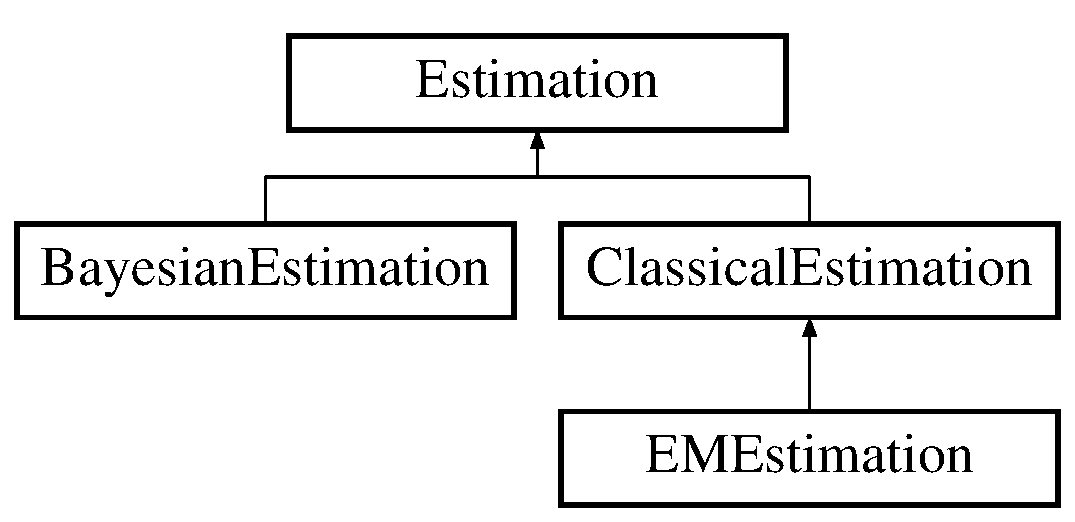
\includegraphics[height=3.000000cm]{classEstimation}
\end{center}
\end{figure}
\subsection*{Public Member Functions}
\begin{DoxyCompactItemize}
\item 
virtual void \hyperlink{classEstimation_ab637475bb8ae37f256c94f7b3cdbe848}{estimate} ()=0
\item 
virtual void \hyperlink{classEstimation_a65f0bd4b60e82a2ab374abd687c69caa}{set\+Model} (\hyperlink{classModel}{Model} $\ast$)=0
\item 
virtual \hyperlink{classEstimation_a4f236659f3afc3db2ee3b6cececc7ce9}{$\sim$\+Estimation} ()
\end{DoxyCompactItemize}
\subsection*{Protected Attributes}
\begin{DoxyCompactItemize}
\item 
\hyperlink{classModel}{Model} $\ast$ \hyperlink{classEstimation_a3ee97aaf032f3522a294d934c138b29a}{model}
\end{DoxyCompactItemize}


\subsection{Detailed Description}
Parent estimation interface for all estimation methods. 

Definition at line 19 of file Estimation.\+h.



\subsection{Constructor \& Destructor Documentation}
\hypertarget{classEstimation_a4f236659f3afc3db2ee3b6cececc7ce9}{}\index{Estimation@{Estimation}!````~Estimation@{$\sim$\+Estimation}}
\index{````~Estimation@{$\sim$\+Estimation}!Estimation@{Estimation}}
\subsubsection[{$\sim$\+Estimation}]{\setlength{\rightskip}{0pt plus 5cm}Estimation\+::$\sim$\+Estimation (
\begin{DoxyParamCaption}
{}
\end{DoxyParamCaption}
)\hspace{0.3cm}{\ttfamily [virtual]}}\label{classEstimation_a4f236659f3afc3db2ee3b6cececc7ce9}


Definition at line 10 of file Estimation.\+cpp.



\subsection{Member Function Documentation}
\hypertarget{classEstimation_ab637475bb8ae37f256c94f7b3cdbe848}{}\index{Estimation@{Estimation}!estimate@{estimate}}
\index{estimate@{estimate}!Estimation@{Estimation}}
\subsubsection[{estimate}]{\setlength{\rightskip}{0pt plus 5cm}virtual void Estimation\+::estimate (
\begin{DoxyParamCaption}
{}
\end{DoxyParamCaption}
)\hspace{0.3cm}{\ttfamily [pure virtual]}}\label{classEstimation_ab637475bb8ae37f256c94f7b3cdbe848}


Implemented in \hyperlink{classEMEstimation_a7391808764fd510d6a0f0351ec699b2d}{E\+M\+Estimation}, \hyperlink{classClassicalEstimation_a182aef8049a48cf1bd09bff642df8c01}{Classical\+Estimation}, and \hyperlink{classBayesianEstimation_a363ef2a057fe5b20f8724a7ddbb3463b}{Bayesian\+Estimation}.

\hypertarget{classEstimation_a65f0bd4b60e82a2ab374abd687c69caa}{}\index{Estimation@{Estimation}!set\+Model@{set\+Model}}
\index{set\+Model@{set\+Model}!Estimation@{Estimation}}
\subsubsection[{set\+Model}]{\setlength{\rightskip}{0pt plus 5cm}virtual void Estimation\+::set\+Model (
\begin{DoxyParamCaption}
\item[{{\bf Model} $\ast$}]{}
\end{DoxyParamCaption}
)\hspace{0.3cm}{\ttfamily [pure virtual]}}\label{classEstimation_a65f0bd4b60e82a2ab374abd687c69caa}


Implemented in \hyperlink{classEMEstimation_a6cd3ac7193ff9d5d92bd90b58da26e11}{E\+M\+Estimation}, \hyperlink{classClassicalEstimation_a4add5ad245795b82380af0c34840c603}{Classical\+Estimation}, and \hyperlink{classBayesianEstimation_a46020e91ec07e5e81560fa159a37be16}{Bayesian\+Estimation}.



\subsection{Member Data Documentation}
\hypertarget{classEstimation_a3ee97aaf032f3522a294d934c138b29a}{}\index{Estimation@{Estimation}!model@{model}}
\index{model@{model}!Estimation@{Estimation}}
\subsubsection[{model}]{\setlength{\rightskip}{0pt plus 5cm}{\bf Model}$\ast$ Estimation\+::model\hspace{0.3cm}{\ttfamily [protected]}}\label{classEstimation_a3ee97aaf032f3522a294d934c138b29a}


Definition at line 21 of file Estimation.\+h.



The documentation for this class was generated from the following files\+:\begin{DoxyCompactItemize}
\item 
src/estimation/\hyperlink{Estimation_8h}{Estimation.\+h}\item 
src/estimation/\hyperlink{Estimation_8cpp}{Estimation.\+cpp}\end{DoxyCompactItemize}

\hypertarget{classExpectation}{}\section{Expectation Class Reference}
\label{classExpectation}\index{Expectation@{Expectation}}


{\ttfamily \#include $<$Expectation.\+h$>$}

\subsection*{Public Member Functions}
\begin{DoxyCompactItemize}
\item 
\hyperlink{classExpectation_ab0567960d034da8603372199997608ea}{Expectation} ()
\item 
virtual \hyperlink{classExpectation_a3d332bb680bdd4ace5df67279bb9b55f}{$\sim$\+Expectation} ()
\end{DoxyCompactItemize}


\subsection{Detailed Description}


Definition at line 11 of file Expectation.\+h.



\subsection{Constructor \& Destructor Documentation}
\hypertarget{classExpectation_ab0567960d034da8603372199997608ea}{}\index{Expectation@{Expectation}!Expectation@{Expectation}}
\index{Expectation@{Expectation}!Expectation@{Expectation}}
\subsubsection[{Expectation}]{\setlength{\rightskip}{0pt plus 5cm}Expectation\+::\+Expectation (
\begin{DoxyParamCaption}
{}
\end{DoxyParamCaption}
)}\label{classExpectation_ab0567960d034da8603372199997608ea}


Definition at line 10 of file Expectation.\+cpp.

\hypertarget{classExpectation_a3d332bb680bdd4ace5df67279bb9b55f}{}\index{Expectation@{Expectation}!````~Expectation@{$\sim$\+Expectation}}
\index{````~Expectation@{$\sim$\+Expectation}!Expectation@{Expectation}}
\subsubsection[{$\sim$\+Expectation}]{\setlength{\rightskip}{0pt plus 5cm}Expectation\+::$\sim$\+Expectation (
\begin{DoxyParamCaption}
{}
\end{DoxyParamCaption}
)\hspace{0.3cm}{\ttfamily [virtual]}}\label{classExpectation_a3d332bb680bdd4ace5df67279bb9b55f}


Definition at line 15 of file Expectation.\+cpp.



The documentation for this class was generated from the following files\+:\begin{DoxyCompactItemize}
\item 
src/util/\hyperlink{Expectation_8h}{Expectation.\+h}\item 
src/util/\hyperlink{Expectation_8cpp}{Expectation.\+cpp}\end{DoxyCompactItemize}

\hypertarget{classFisherScoringOptimizer}{}\section{Fisher\+Scoring\+Optimizer Class Reference}
\label{classFisherScoringOptimizer}\index{Fisher\+Scoring\+Optimizer@{Fisher\+Scoring\+Optimizer}}


Skeleton for implementing the Fisher \hyperlink{classOptimizer}{Optimizer}.  




{\ttfamily \#include $<$Fisher\+Scoring\+Optimizer.\+h$>$}



\subsection{Detailed Description}
Skeleton for implementing the Fisher \hyperlink{classOptimizer}{Optimizer}. 

Definition at line 13 of file Fisher\+Scoring\+Optimizer.\+h.



The documentation for this class was generated from the following file\+:\begin{DoxyCompactItemize}
\item 
src/optimizer/\hyperlink{FisherScoringOptimizer_8h}{Fisher\+Scoring\+Optimizer.\+h}\end{DoxyCompactItemize}

\hypertarget{classInput}{}\section{Input Class Reference}
\label{classInput}\index{Input@{Input}}


Class that is in charge of taking O\+S files, streams and other sources for inputting data into the software suite.  




{\ttfamily \#include $<$Input.\+h$>$}

\subsection*{Public Member Functions}
\begin{DoxyCompactItemize}
\item 
\hyperlink{classInput_abae3f379d3f157cf42dc857309832dba}{Input} ()
\item 
virtual \hyperlink{classInput_af2db35ba67c8a8ccd23bef6a482fc291}{$\sim$\+Input} ()
\item 
bool \hyperlink{classInput_ae2c34c38d697cdad30398d120e61579f}{import\+C\+S\+V} (char $\ast$, \hyperlink{classPatternMatrix}{Pattern\+Matrix} \&, unsigned int, unsigned int)
\item 
bool \hyperlink{classInput_a6d05f89d9f355f475974cf1bd92c9054}{import\+C\+S\+V} (char $\ast$, \hyperlink{singletonMatrix}{Matrix}$<$ double $>$ \&, unsigned int, unsigned int)
\begin{DoxyCompactList}\small\item\em Imports binary matrices from a csv. \end{DoxyCompactList}\item 
char \hyperlink{classInput_a361b89353087aa7f962a7bf748923239}{get\+Del} () const 
\begin{DoxyCompactList}\small\item\em Imports generic type matrices from a csv. \end{DoxyCompactList}\item 
void \hyperlink{classInput_a6303c6ebccb76588fb55a8bdb6b1f9ab}{set\+Del} (char)
\begin{DoxyCompactList}\small\item\em Gets the delimitier used for inputting. \end{DoxyCompactList}\end{DoxyCompactItemize}
\subsection*{Private Attributes}
\begin{DoxyCompactItemize}
\item 
char \hyperlink{classInput_aeecf320ec4c73b68165b8c19a6a3d28a}{del}
\end{DoxyCompactItemize}


\subsection{Detailed Description}
Class that is in charge of taking O\+S files, streams and other sources for inputting data into the software suite. 

Definition at line 28 of file Input.\+h.



\subsection{Constructor \& Destructor Documentation}
\hypertarget{classInput_abae3f379d3f157cf42dc857309832dba}{}\index{Input@{Input}!Input@{Input}}
\index{Input@{Input}!Input@{Input}}
\subsubsection[{Input}]{\setlength{\rightskip}{0pt plus 5cm}Input\+::\+Input (
\begin{DoxyParamCaption}
{}
\end{DoxyParamCaption}
)}\label{classInput_abae3f379d3f157cf42dc857309832dba}


Definition at line 10 of file Input.\+cpp.



References del.

\hypertarget{classInput_af2db35ba67c8a8ccd23bef6a482fc291}{}\index{Input@{Input}!````~Input@{$\sim$\+Input}}
\index{````~Input@{$\sim$\+Input}!Input@{Input}}
\subsubsection[{$\sim$\+Input}]{\setlength{\rightskip}{0pt plus 5cm}Input\+::$\sim$\+Input (
\begin{DoxyParamCaption}
{}
\end{DoxyParamCaption}
)\hspace{0.3cm}{\ttfamily [virtual]}}\label{classInput_af2db35ba67c8a8ccd23bef6a482fc291}


Definition at line 15 of file Input.\+cpp.



\subsection{Member Function Documentation}
\hypertarget{classInput_a361b89353087aa7f962a7bf748923239}{}\index{Input@{Input}!get\+Del@{get\+Del}}
\index{get\+Del@{get\+Del}!Input@{Input}}
\subsubsection[{get\+Del}]{\setlength{\rightskip}{0pt plus 5cm}char Input\+::get\+Del (
\begin{DoxyParamCaption}
{}
\end{DoxyParamCaption}
) const}\label{classInput_a361b89353087aa7f962a7bf748923239}


Imports generic type matrices from a csv. 



Definition at line 169 of file Input.\+cpp.



References del.

\hypertarget{classInput_ae2c34c38d697cdad30398d120e61579f}{}\index{Input@{Input}!import\+C\+S\+V@{import\+C\+S\+V}}
\index{import\+C\+S\+V@{import\+C\+S\+V}!Input@{Input}}
\subsubsection[{import\+C\+S\+V}]{\setlength{\rightskip}{0pt plus 5cm}bool Input\+::import\+C\+S\+V (
\begin{DoxyParamCaption}
\item[{char $\ast$}]{filename, }
\item[{{\bf Pattern\+Matrix} \&}]{M, }
\item[{unsigned int}]{row\+Idx, }
\item[{unsigned int}]{col\+Idx}
\end{DoxyParamCaption}
)}\label{classInput_ae2c34c38d697cdad30398d120e61579f}


Definition at line 85 of file Input.\+cpp.



References del, and Pattern\+Matrix\+::push().



Referenced by one\+Run(), and pachotest().

\hypertarget{classInput_a6d05f89d9f355f475974cf1bd92c9054}{}\index{Input@{Input}!import\+C\+S\+V@{import\+C\+S\+V}}
\index{import\+C\+S\+V@{import\+C\+S\+V}!Input@{Input}}
\subsubsection[{import\+C\+S\+V}]{\setlength{\rightskip}{0pt plus 5cm}bool Input\+::import\+C\+S\+V (
\begin{DoxyParamCaption}
\item[{char $\ast$}]{filename, }
\item[{{\bf Matrix}$<$ double $>$ \&}]{M, }
\item[{unsigned int}]{row\+Idx, }
\item[{unsigned int}]{col\+Idx}
\end{DoxyParamCaption}
)}\label{classInput_a6d05f89d9f355f475974cf1bd92c9054}


Imports binary matrices from a csv. 



Definition at line 18 of file Input.\+cpp.



References del.

\hypertarget{classInput_a6303c6ebccb76588fb55a8bdb6b1f9ab}{}\index{Input@{Input}!set\+Del@{set\+Del}}
\index{set\+Del@{set\+Del}!Input@{Input}}
\subsubsection[{set\+Del}]{\setlength{\rightskip}{0pt plus 5cm}void Input\+::set\+Del (
\begin{DoxyParamCaption}
\item[{char}]{del}
\end{DoxyParamCaption}
)}\label{classInput_a6303c6ebccb76588fb55a8bdb6b1f9ab}


Gets the delimitier used for inputting. 



Definition at line 173 of file Input.\+cpp.



References del.



\subsection{Member Data Documentation}
\hypertarget{classInput_aeecf320ec4c73b68165b8c19a6a3d28a}{}\index{Input@{Input}!del@{del}}
\index{del@{del}!Input@{Input}}
\subsubsection[{del}]{\setlength{\rightskip}{0pt plus 5cm}char Input\+::del\hspace{0.3cm}{\ttfamily [private]}}\label{classInput_aeecf320ec4c73b68165b8c19a6a3d28a}


Definition at line 34 of file Input.\+h.



Referenced by get\+Del(), import\+C\+S\+V(), Input(), and set\+Del().



The documentation for this class was generated from the following files\+:\begin{DoxyCompactItemize}
\item 
src/input/\hyperlink{Input_8h}{Input.\+h}\item 
src/input/\hyperlink{Input_8cpp}{Input.\+cpp}\end{DoxyCompactItemize}

\hypertarget{classItemModel}{}\section{Item\+Model Class Reference}
\label{classItemModel}\index{Item\+Model@{Item\+Model}}


{\ttfamily \#include $<$Item\+Model.\+h$>$}

Inheritance diagram for Item\+Model\+:\begin{figure}[H]
\begin{center}
\leavevmode
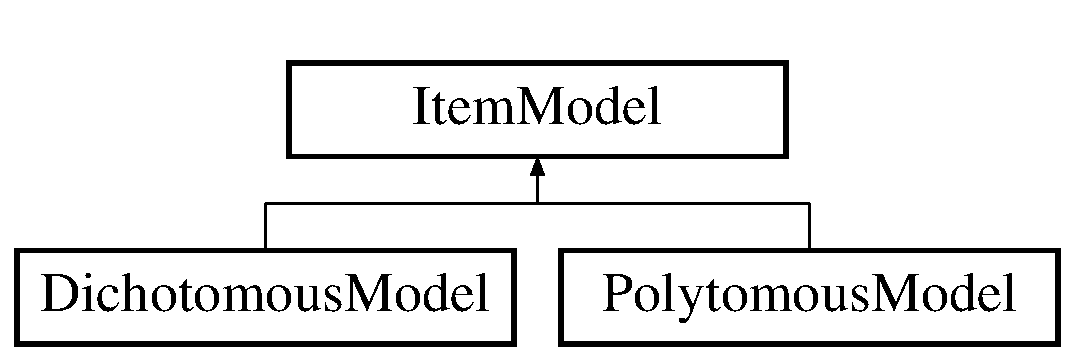
\includegraphics[height=2.000000cm]{classItemModel}
\end{center}
\end{figure}
\subsection*{Public Member Functions}
\begin{DoxyCompactItemize}
\item 
virtual int \hyperlink{classItemModel_af0aabe9f48c6d111fbcb903cb330fae7}{count\+Categories} ()=0
\item 
virtual int \hyperlink{classItemModel_a7a93c60e346f4d80f265a4c9e083181d}{count\+Items} ()=0
\item 
virtual \hyperlink{classDataSet}{Data\+Set} $\ast$ \hyperlink{classItemModel_a8521ea3f8f511e88d5257ff7591cd928}{get\+Dataset} ()=0
\item 
virtual void \hyperlink{classItemModel_accd6c6b6827c45970d04c22baaca6b0c}{set\+Dataset} (\hyperlink{classDataSet}{Data\+Set} $\ast$dataset)=0
\item 
virtual \hyperlink{classItemModel_ac824a8715e939060d4efdee0949d02cf}{$\sim$\+Item\+Model} ()
\end{DoxyCompactItemize}
\subsection*{Protected Attributes}
\begin{DoxyCompactItemize}
\item 
\hyperlink{classDataSet}{Data\+Set} $\ast$ \hyperlink{classItemModel_a160f86bf5a0eba987f4c8a8499e448a6}{data\+Set}
\end{DoxyCompactItemize}


\subsection{Detailed Description}


Definition at line 13 of file Item\+Model.\+h.



\subsection{Constructor \& Destructor Documentation}
\hypertarget{classItemModel_ac824a8715e939060d4efdee0949d02cf}{}\index{Item\+Model@{Item\+Model}!````~Item\+Model@{$\sim$\+Item\+Model}}
\index{````~Item\+Model@{$\sim$\+Item\+Model}!Item\+Model@{Item\+Model}}
\subsubsection[{$\sim$\+Item\+Model}]{\setlength{\rightskip}{0pt plus 5cm}Item\+Model\+::$\sim$\+Item\+Model (
\begin{DoxyParamCaption}
{}
\end{DoxyParamCaption}
)\hspace{0.3cm}{\ttfamily [virtual]}}\label{classItemModel_ac824a8715e939060d4efdee0949d02cf}


Definition at line 11 of file Item\+Model.\+cpp.



\subsection{Member Function Documentation}
\hypertarget{classItemModel_af0aabe9f48c6d111fbcb903cb330fae7}{}\index{Item\+Model@{Item\+Model}!count\+Categories@{count\+Categories}}
\index{count\+Categories@{count\+Categories}!Item\+Model@{Item\+Model}}
\subsubsection[{count\+Categories}]{\setlength{\rightskip}{0pt plus 5cm}virtual int Item\+Model\+::count\+Categories (
\begin{DoxyParamCaption}
{}
\end{DoxyParamCaption}
)\hspace{0.3cm}{\ttfamily [pure virtual]}}\label{classItemModel_af0aabe9f48c6d111fbcb903cb330fae7}


Implemented in \hyperlink{classDichotomousModel_a6861f3ef96b4525ba1b1db1a7dfb1ca3}{Dichotomous\+Model}, and \hyperlink{classPolytomousModel_a1a65e5771d53f6921c48fdc41ea62961}{Polytomous\+Model}.

\hypertarget{classItemModel_a7a93c60e346f4d80f265a4c9e083181d}{}\index{Item\+Model@{Item\+Model}!count\+Items@{count\+Items}}
\index{count\+Items@{count\+Items}!Item\+Model@{Item\+Model}}
\subsubsection[{count\+Items}]{\setlength{\rightskip}{0pt plus 5cm}virtual int Item\+Model\+::count\+Items (
\begin{DoxyParamCaption}
{}
\end{DoxyParamCaption}
)\hspace{0.3cm}{\ttfamily [pure virtual]}}\label{classItemModel_a7a93c60e346f4d80f265a4c9e083181d}


Implemented in \hyperlink{classDichotomousModel_ae9dfca33b3549ea73e4fc8fcab204cc0}{Dichotomous\+Model}, and \hyperlink{classPolytomousModel_a8828b2108445ef361a4af0a3aaf07e86}{Polytomous\+Model}.



Referenced by Three\+P\+L\+Model\+::build\+Parameter\+Set(), E\+M\+Estimation\+::estimate(), one\+Run(), and E\+M\+Estimation\+::set\+Model().

\hypertarget{classItemModel_a8521ea3f8f511e88d5257ff7591cd928}{}\index{Item\+Model@{Item\+Model}!get\+Dataset@{get\+Dataset}}
\index{get\+Dataset@{get\+Dataset}!Item\+Model@{Item\+Model}}
\subsubsection[{get\+Dataset}]{\setlength{\rightskip}{0pt plus 5cm}virtual {\bf Data\+Set}$\ast$ Item\+Model\+::get\+Dataset (
\begin{DoxyParamCaption}
{}
\end{DoxyParamCaption}
)\hspace{0.3cm}{\ttfamily [pure virtual]}}\label{classItemModel_a8521ea3f8f511e88d5257ff7591cd928}


Implemented in \hyperlink{classDichotomousModel_a0fd6d3ed3a6e78f7a65caa9d2828c7c6}{Dichotomous\+Model}, and \hyperlink{classPolytomousModel_a0e1aa66768478466b3e49a9f54ace8ba}{Polytomous\+Model}.



Referenced by E\+M\+Estimation\+::step\+E(), and E\+M\+Estimation\+::step\+M().

\hypertarget{classItemModel_accd6c6b6827c45970d04c22baaca6b0c}{}\index{Item\+Model@{Item\+Model}!set\+Dataset@{set\+Dataset}}
\index{set\+Dataset@{set\+Dataset}!Item\+Model@{Item\+Model}}
\subsubsection[{set\+Dataset}]{\setlength{\rightskip}{0pt plus 5cm}virtual void Item\+Model\+::set\+Dataset (
\begin{DoxyParamCaption}
\item[{{\bf Data\+Set} $\ast$}]{dataset}
\end{DoxyParamCaption}
)\hspace{0.3cm}{\ttfamily [pure virtual]}}\label{classItemModel_accd6c6b6827c45970d04c22baaca6b0c}


Implemented in \hyperlink{classDichotomousModel_a5e7bf92bc598e581477b9c5814ca7f72}{Dichotomous\+Model}, and \hyperlink{classPolytomousModel_a71b943b552ae6842f94370698fc9ba0b}{Polytomous\+Model}.



Referenced by one\+Run().



\subsection{Member Data Documentation}
\hypertarget{classItemModel_a160f86bf5a0eba987f4c8a8499e448a6}{}\index{Item\+Model@{Item\+Model}!data\+Set@{data\+Set}}
\index{data\+Set@{data\+Set}!Item\+Model@{Item\+Model}}
\subsubsection[{data\+Set}]{\setlength{\rightskip}{0pt plus 5cm}{\bf Data\+Set}$\ast$ Item\+Model\+::data\+Set\hspace{0.3cm}{\ttfamily [protected]}}\label{classItemModel_a160f86bf5a0eba987f4c8a8499e448a6}


Definition at line 15 of file Item\+Model.\+h.



Referenced by Dichotomous\+Model\+::count\+Items(), Polytomous\+Model\+::get\+Dataset(), Dichotomous\+Model\+::get\+Dataset(), Polytomous\+Model\+::set\+Dataset(), and Dichotomous\+Model\+::set\+Dataset().



The documentation for this class was generated from the following files\+:\begin{DoxyCompactItemize}
\item 
src/model/item/\hyperlink{ItemModel_8h}{Item\+Model.\+h}\item 
src/model/item/\hyperlink{ItemModel_8cpp}{Item\+Model.\+cpp}\end{DoxyCompactItemize}

\hypertarget{classLatentTraitSet}{}\section{Latent\+Trait\+Set Class Reference}
\label{classLatentTraitSet}\index{Latent\+Trait\+Set@{Latent\+Trait\+Set}}


{\ttfamily \#include $<$Latent\+Trait\+Set.\+h$>$}

\subsection*{Public Member Functions}
\begin{DoxyCompactItemize}
\item 
\hyperlink{classLatentTraitSet_ae11a4a1e289c42f54179ee47a4fd2ab2}{Latent\+Trait\+Set} ()
\item 
\hyperlink{singletonMatrix}{Matrix}$<$ double $>$ $\ast$ \hyperlink{classLatentTraitSet_aed95a0c5c87256960ffb528ca491f2c0}{get\+Theta} ()
\item 
void \hyperlink{classLatentTraitSet_af8133cfb7853d19f0490079ebc146b6c}{set\+Theta} (\hyperlink{singletonMatrix}{Matrix}$<$ double $>$ $\ast$\hyperlink{classLatentTraitSet_a8e5ce0fbc5b17577bcd06b58d3c5b079}{theta})
\item 
\hyperlink{singletonMatrix}{Matrix}$<$ double $>$ $\ast$ \hyperlink{classLatentTraitSet_a1f48623a0834d134df2ddea3892a5b11}{get\+Weight} ()
\item 
void \hyperlink{classLatentTraitSet_a8a3c362f857d4094f7e2da4f47a9499b}{set\+Weight} (\hyperlink{singletonMatrix}{Matrix}$<$ double $>$ $\ast$\hyperlink{classLatentTraitSet_a8db0053af1838ab0a4e25d5c6abc4384}{weight})
\item 
virtual \hyperlink{classLatentTraitSet_ab502c9823e8c7ed995b0d87d1af94aee}{$\sim$\+Latent\+Trait\+Set} ()
\end{DoxyCompactItemize}
\subsection*{Private Attributes}
\begin{DoxyCompactItemize}
\item 
\hyperlink{singletonMatrix}{Matrix}$<$ double $>$ $\ast$ \hyperlink{classLatentTraitSet_a8e5ce0fbc5b17577bcd06b58d3c5b079}{theta}
\item 
\hyperlink{singletonMatrix}{Matrix}$<$ double $>$ $\ast$ \hyperlink{classLatentTraitSet_a8db0053af1838ab0a4e25d5c6abc4384}{weight}
\end{DoxyCompactItemize}


\subsection{Detailed Description}


Definition at line 13 of file Latent\+Trait\+Set.\+h.



\subsection{Constructor \& Destructor Documentation}
\hypertarget{classLatentTraitSet_ae11a4a1e289c42f54179ee47a4fd2ab2}{}\index{Latent\+Trait\+Set@{Latent\+Trait\+Set}!Latent\+Trait\+Set@{Latent\+Trait\+Set}}
\index{Latent\+Trait\+Set@{Latent\+Trait\+Set}!Latent\+Trait\+Set@{Latent\+Trait\+Set}}
\subsubsection[{Latent\+Trait\+Set}]{\setlength{\rightskip}{0pt plus 5cm}Latent\+Trait\+Set\+::\+Latent\+Trait\+Set (
\begin{DoxyParamCaption}
{}
\end{DoxyParamCaption}
)}\label{classLatentTraitSet_ae11a4a1e289c42f54179ee47a4fd2ab2}


Definition at line 10 of file Latent\+Trait\+Set.\+cpp.



References theta, and weight.

\hypertarget{classLatentTraitSet_ab502c9823e8c7ed995b0d87d1af94aee}{}\index{Latent\+Trait\+Set@{Latent\+Trait\+Set}!````~Latent\+Trait\+Set@{$\sim$\+Latent\+Trait\+Set}}
\index{````~Latent\+Trait\+Set@{$\sim$\+Latent\+Trait\+Set}!Latent\+Trait\+Set@{Latent\+Trait\+Set}}
\subsubsection[{$\sim$\+Latent\+Trait\+Set}]{\setlength{\rightskip}{0pt plus 5cm}Latent\+Trait\+Set\+::$\sim$\+Latent\+Trait\+Set (
\begin{DoxyParamCaption}
{}
\end{DoxyParamCaption}
)\hspace{0.3cm}{\ttfamily [virtual]}}\label{classLatentTraitSet_ab502c9823e8c7ed995b0d87d1af94aee}


Definition at line 31 of file Latent\+Trait\+Set.\+cpp.



References theta, and weight.



\subsection{Member Function Documentation}
\hypertarget{classLatentTraitSet_aed95a0c5c87256960ffb528ca491f2c0}{}\index{Latent\+Trait\+Set@{Latent\+Trait\+Set}!get\+Theta@{get\+Theta}}
\index{get\+Theta@{get\+Theta}!Latent\+Trait\+Set@{Latent\+Trait\+Set}}
\subsubsection[{get\+Theta}]{\setlength{\rightskip}{0pt plus 5cm}{\bf Matrix}$<$ double $>$ $\ast$ Latent\+Trait\+Set\+::get\+Theta (
\begin{DoxyParamCaption}
{}
\end{DoxyParamCaption}
)}\label{classLatentTraitSet_aed95a0c5c87256960ffb528ca491f2c0}


Definition at line 15 of file Latent\+Trait\+Set.\+cpp.



References theta.



Referenced by Three\+P\+L\+Model\+::build\+Parameter\+Set(), Unidimensional\+Model\+::get\+Dim\+Vector(), E\+M\+Estimation\+::set\+Model(), E\+M\+Estimation\+::step\+E(), E\+M\+Estimation\+::step\+M(), and Three\+P\+L\+Model\+::success\+Probability().

\hypertarget{classLatentTraitSet_a1f48623a0834d134df2ddea3892a5b11}{}\index{Latent\+Trait\+Set@{Latent\+Trait\+Set}!get\+Weight@{get\+Weight}}
\index{get\+Weight@{get\+Weight}!Latent\+Trait\+Set@{Latent\+Trait\+Set}}
\subsubsection[{get\+Weight}]{\setlength{\rightskip}{0pt plus 5cm}{\bf Matrix}$<$ double $>$ $\ast$ Latent\+Trait\+Set\+::get\+Weight (
\begin{DoxyParamCaption}
{}
\end{DoxyParamCaption}
)}\label{classLatentTraitSet_a1f48623a0834d134df2ddea3892a5b11}


Definition at line 23 of file Latent\+Trait\+Set.\+cpp.



References weight.



Referenced by E\+M\+Estimation\+::step\+E().

\hypertarget{classLatentTraitSet_af8133cfb7853d19f0490079ebc146b6c}{}\index{Latent\+Trait\+Set@{Latent\+Trait\+Set}!set\+Theta@{set\+Theta}}
\index{set\+Theta@{set\+Theta}!Latent\+Trait\+Set@{Latent\+Trait\+Set}}
\subsubsection[{set\+Theta}]{\setlength{\rightskip}{0pt plus 5cm}void Latent\+Trait\+Set\+::set\+Theta (
\begin{DoxyParamCaption}
\item[{{\bf Matrix}$<$ double $>$ $\ast$}]{theta}
\end{DoxyParamCaption}
)}\label{classLatentTraitSet_af8133cfb7853d19f0490079ebc146b6c}


Definition at line 19 of file Latent\+Trait\+Set.\+cpp.



References theta.



Referenced by one\+Run().

\hypertarget{classLatentTraitSet_a8a3c362f857d4094f7e2da4f47a9499b}{}\index{Latent\+Trait\+Set@{Latent\+Trait\+Set}!set\+Weight@{set\+Weight}}
\index{set\+Weight@{set\+Weight}!Latent\+Trait\+Set@{Latent\+Trait\+Set}}
\subsubsection[{set\+Weight}]{\setlength{\rightskip}{0pt plus 5cm}void Latent\+Trait\+Set\+::set\+Weight (
\begin{DoxyParamCaption}
\item[{{\bf Matrix}$<$ double $>$ $\ast$}]{weight}
\end{DoxyParamCaption}
)}\label{classLatentTraitSet_a8a3c362f857d4094f7e2da4f47a9499b}


Definition at line 27 of file Latent\+Trait\+Set.\+cpp.



References weight.



Referenced by one\+Run().



\subsection{Member Data Documentation}
\hypertarget{classLatentTraitSet_a8e5ce0fbc5b17577bcd06b58d3c5b079}{}\index{Latent\+Trait\+Set@{Latent\+Trait\+Set}!theta@{theta}}
\index{theta@{theta}!Latent\+Trait\+Set@{Latent\+Trait\+Set}}
\subsubsection[{theta}]{\setlength{\rightskip}{0pt plus 5cm}{\bf Matrix}$<$double$>$$\ast$ Latent\+Trait\+Set\+::theta\hspace{0.3cm}{\ttfamily [private]}}\label{classLatentTraitSet_a8e5ce0fbc5b17577bcd06b58d3c5b079}


Definition at line 14 of file Latent\+Trait\+Set.\+h.



Referenced by get\+Theta(), Latent\+Trait\+Set(), set\+Theta(), and $\sim$\+Latent\+Trait\+Set().

\hypertarget{classLatentTraitSet_a8db0053af1838ab0a4e25d5c6abc4384}{}\index{Latent\+Trait\+Set@{Latent\+Trait\+Set}!weight@{weight}}
\index{weight@{weight}!Latent\+Trait\+Set@{Latent\+Trait\+Set}}
\subsubsection[{weight}]{\setlength{\rightskip}{0pt plus 5cm}{\bf Matrix}$<$double$>$$\ast$ Latent\+Trait\+Set\+::weight\hspace{0.3cm}{\ttfamily [private]}}\label{classLatentTraitSet_a8db0053af1838ab0a4e25d5c6abc4384}


Definition at line 15 of file Latent\+Trait\+Set.\+h.



Referenced by get\+Weight(), Latent\+Trait\+Set(), set\+Weight(), and $\sim$\+Latent\+Trait\+Set().



The documentation for this class was generated from the following files\+:\begin{DoxyCompactItemize}
\item 
src/type/\hyperlink{LatentTraitSet_8h}{Latent\+Trait\+Set.\+h}\item 
src/type/\hyperlink{LatentTraitSet_8cpp}{Latent\+Trait\+Set.\+cpp}\end{DoxyCompactItemize}

\hypertarget{structmatrix}{}\section{matrix Struct Reference}
\label{structmatrix}\index{matrix@{matrix}}


{\ttfamily \#include $<$N\+C\+M.\+h$>$}

\subsection*{Public Attributes}
\begin{DoxyCompactItemize}
\item 
double $\ast$ \hyperlink{structmatrix_a720057f595a0b775b6d7d8c9badaca78}{entries}
\item 
int \hyperlink{structmatrix_af83737a5597214de0458c5535a787143}{rows}
\item 
int \hyperlink{structmatrix_a69a002417ab248fe46a11badaaede9ef}{columns}
\end{DoxyCompactItemize}


\subsection{Detailed Description}


Definition at line 63 of file N\+C\+M.\+h.



\subsection{Member Data Documentation}
\hypertarget{structmatrix_a69a002417ab248fe46a11badaaede9ef}{}\index{matrix@{matrix}!columns@{columns}}
\index{columns@{columns}!matrix@{matrix}}
\subsubsection[{columns}]{\setlength{\rightskip}{0pt plus 5cm}int matrix\+::columns}\label{structmatrix_a69a002417ab248fe46a11badaaede9ef}


Definition at line 67 of file N\+C\+M.\+h.



Referenced by Correlation\+\_\+\+Newton(), gradient(), Jacobian\+\_\+matrix(), N\+C\+M(), omega\+\_\+mat(), pre\+\_\+cg(), precond\+\_\+matrix(), and print\+Matrix().

\hypertarget{structmatrix_a720057f595a0b775b6d7d8c9badaca78}{}\index{matrix@{matrix}!entries@{entries}}
\index{entries@{entries}!matrix@{matrix}}
\subsubsection[{entries}]{\setlength{\rightskip}{0pt plus 5cm}double$\ast$ matrix\+::entries}\label{structmatrix_a720057f595a0b775b6d7d8c9badaca78}


Definition at line 65 of file N\+C\+M.\+h.



Referenced by Correlation\+\_\+\+Newton(), gradient(), Jacobian\+\_\+matrix(), N\+C\+M(), omega\+\_\+mat(), pre\+\_\+cg(), precond\+\_\+matrix(), and print\+Matrix().

\hypertarget{structmatrix_af83737a5597214de0458c5535a787143}{}\index{matrix@{matrix}!rows@{rows}}
\index{rows@{rows}!matrix@{matrix}}
\subsubsection[{rows}]{\setlength{\rightskip}{0pt plus 5cm}int matrix\+::rows}\label{structmatrix_af83737a5597214de0458c5535a787143}


Definition at line 66 of file N\+C\+M.\+h.



Referenced by Correlation\+\_\+\+Newton(), gradient(), Jacobian\+\_\+matrix(), N\+C\+M(), omega\+\_\+mat(), pre\+\_\+cg(), precond\+\_\+matrix(), and print\+Matrix().



The documentation for this struct was generated from the following file\+:\begin{DoxyCompactItemize}
\item 
src/util/\hyperlink{NCM_8h}{N\+C\+M.\+h}\end{DoxyCompactItemize}

\hypertarget{singletonMatrix}{}\section{Matrix$<$ T $>$ Class Template Reference}
\label{singletonMatrix}\index{Matrix$<$ T $>$@{Matrix$<$ T $>$}}


Supports the \hyperlink{singletonMatrix}{Matrix} Structures, with indexing on any type, has special operations for general matrix use, is the class used by all the B\+L\+A\+S interface methods , please use this class in the package whenever posible.  




{\ttfamily \#include $<$Matrix.\+h$>$}

\subsection*{Public Member Functions}
\begin{DoxyCompactItemize}
\item 
\hyperlink{singletonMatrix_a9d567e3a121b1be0c3f9c461cab524fe}{Matrix} ()
\item 
\hyperlink{singletonMatrix_a949022174714dfd05d0352d3fbaf5143}{Matrix} (int, int)
\begin{DoxyCompactList}\small\item\em Empty object. \end{DoxyCompactList}\item 
\hyperlink{singletonMatrix_a15459936dd063e395c33859641155f53}{Matrix} (\hyperlink{singletonMatrix}{Matrix}$<$ T $>$ \&)
\begin{DoxyCompactList}\small\item\em Two dimensional \hyperlink{singletonMatrix}{Matrix} Constructor allocates memory. \end{DoxyCompactList}\item 
\hyperlink{singletonMatrix_a046f07c969647c44e8f7b438e993e321}{Matrix} (char I, int size)
\begin{DoxyCompactList}\small\item\em Copy constructor. \end{DoxyCompactList}\item 
void \hyperlink{singletonMatrix_af40e280112b61f6a37b54d2e5ef02e5b}{reset} ()
\begin{DoxyCompactList}\small\item\em Create special kinds of matrices (dense identity) \end{DoxyCompactList}\item 
void \hyperlink{singletonMatrix_a4b360b44312566fb94cd3e66e7088890}{transpose} ()
\begin{DoxyCompactList}\small\item\em Reset method, puts all entries in zeros. \end{DoxyCompactList}\item 
void \hyperlink{singletonMatrix_a7b8a11a3ab5ab38545d394cc60d0b96c}{copy} (\hyperlink{singletonMatrix}{Matrix}$<$ T $>$ \&)
\begin{DoxyCompactList}\small\item\em Transposes the matrix, notice it does not perform memory transpose, only index transpose. \end{DoxyCompactList}\item 
T \hyperlink{singletonMatrix_a1bf128c2250ee887b61445301ecdf789}{get\+Determinant} ()
\begin{DoxyCompactList}\small\item\em Copy constructor. \end{DoxyCompactList}\item 
int \hyperlink{singletonMatrix_a8e38d0aac1a8a82ae00e2fb5328b114c}{n\+R} ()
\begin{DoxyCompactList}\small\item\em Outputs the determinant of the matrix. \end{DoxyCompactList}\item 
int \hyperlink{singletonMatrix_abe6a17af941c66a1cceade934996c696}{n\+C} ()
\begin{DoxyCompactList}\small\item\em Returns number of rows. \end{DoxyCompactList}\item 
T \hyperlink{singletonMatrix_a00f833a52561b2665f3e93f254d363ac}{sum} ()
\begin{DoxyCompactList}\small\item\em Returns number of columns. \end{DoxyCompactList}\item 
T \& \hyperlink{singletonMatrix_a3f74c738d77726e6e63b61cc8ee19525}{operator()} (const int \hyperlink{singletonMatrix_aa3b73b40cb492b1a2b73c94fc5c3e212}{n\+Col}, const int \hyperlink{singletonMatrix_a18ad6163c76247e0c007c48d18e62afa}{n\+Row})
\begin{DoxyCompactList}\small\item\em Returns the sum of all objects. \end{DoxyCompactList}\item 
T \& \hyperlink{singletonMatrix_ab490c4125fa561019bdc81cf7c55b02a}{operator()} (const int element)
\begin{DoxyCompactList}\small\item\em Accessing operator for a element. \end{DoxyCompactList}\item 
bool \hyperlink{singletonMatrix_abe9c889826b481f9bd55b692df4caaf4}{is\+Symmetric} () const 
\begin{DoxyCompactList}\small\item\em \hyperlink{classOutput}{Output} operator. \end{DoxyCompactList}\item 
void \hyperlink{singletonMatrix_a384a4255276f138ce28dc2718cbd35a1}{set\+Symmetric} (bool \hyperlink{singletonMatrix_af2bf28cc007514273c14f89975438701}{symmetric})
\begin{DoxyCompactList}\small\item\em Symmetry flag for optimizations. \end{DoxyCompactList}\item 
virtual \hyperlink{singletonMatrix_a91aa704de674203e96aece9e1955ccd3}{$\sim$\+Matrix} ()
\begin{DoxyCompactList}\small\item\em Set to true the symmetry flag. \end{DoxyCompactList}\end{DoxyCompactItemize}
\subsection*{Public Attributes}
\begin{DoxyCompactItemize}
\item 
bool \hyperlink{singletonMatrix_aa9511b2f62fafa982819c9d22b4fbefc}{transposed}
\item 
bool \hyperlink{singletonMatrix_af2bf28cc007514273c14f89975438701}{symmetric}
\item 
T $\ast$ \hyperlink{singletonMatrix_ae50290f97073a6d396def5da5b36d811}{memory}
\item 
int \hyperlink{singletonMatrix_ac0297673d046ad5f9eaa4d621a95d6c8}{ld}
\end{DoxyCompactItemize}
\subsection*{Static Public Attributes}
\begin{DoxyCompactItemize}
\item 
static char \hyperlink{singletonMatrix_a97c4971ed81b3fe5aa55c05cd5ec7a4b}{del} = ' '
\end{DoxyCompactItemize}
\subsection*{Private Member Functions}
\begin{DoxyCompactItemize}
\item 
T \hyperlink{singletonMatrix_a9074cd1c4e1d995ba8267667868ac753}{m} (char)
\item 
T \hyperlink{singletonMatrix_ae6b5e83d3161ce069b86717c90ed0ea5}{get3x3determinant} ()
\end{DoxyCompactItemize}
\subsection*{Private Attributes}
\begin{DoxyCompactItemize}
\item 
int \hyperlink{singletonMatrix_aa3b73b40cb492b1a2b73c94fc5c3e212}{n\+Col}
\item 
int \hyperlink{singletonMatrix_a18ad6163c76247e0c007c48d18e62afa}{n\+Row}
\end{DoxyCompactItemize}
\subsection*{Friends}
\begin{DoxyCompactItemize}
\item 
ostream \& \hyperlink{singletonMatrix_abbea375d42e57221a552685b6bb1372f}{operator} (ostream \&, \hyperlink{singletonMatrix}{Matrix}$<$ T $>$ \&)
\begin{DoxyCompactList}\small\item\em Accessing operator for a element. \end{DoxyCompactList}\end{DoxyCompactItemize}


\subsection{Detailed Description}
\subsubsection*{template$<$class T$>$class Matrix$<$ T $>$}

Supports the \hyperlink{singletonMatrix}{Matrix} Structures, with indexing on any type, has special operations for general matrix use, is the class used by all the B\+L\+A\+S interface methods , please use this class in the package whenever posible. 

the class is a templated class supporting any type for components of the matrix, the support of this class is made for two dimension matrices and one dimension vectors, overloaded operators are the parenthesis for one or two dimensional indexing, and the output operator, the class also supports transposed and symmetric matrices and when declaring matrices they can be declared either empty, reseted to a value, as an identity, or as a random matrix. Some very fast methods are implemented for specific matrix sizes. Use this with care. 

Definition at line 31 of file Matrix.\+h.



\subsection{Constructor \& Destructor Documentation}
\hypertarget{singletonMatrix_a9d567e3a121b1be0c3f9c461cab524fe}{}\index{Matrix@{Matrix}!Matrix@{Matrix}}
\index{Matrix@{Matrix}!Matrix@{Matrix}}
\subsubsection[{Matrix}]{\setlength{\rightskip}{0pt plus 5cm}template$<$class T $>$ {\bf Matrix}$<$ T $>$\+::{\bf Matrix} (
\begin{DoxyParamCaption}
{}
\end{DoxyParamCaption}
)}\label{singletonMatrix_a9d567e3a121b1be0c3f9c461cab524fe}


Definition at line 102 of file Matrix.\+h.

\hypertarget{singletonMatrix_a949022174714dfd05d0352d3fbaf5143}{}\index{Matrix@{Matrix}!Matrix@{Matrix}}
\index{Matrix@{Matrix}!Matrix@{Matrix}}
\subsubsection[{Matrix}]{\setlength{\rightskip}{0pt plus 5cm}template$<$class T $>$ {\bf Matrix}$<$ T $>$\+::{\bf Matrix} (
\begin{DoxyParamCaption}
\item[{int}]{r, }
\item[{int}]{c}
\end{DoxyParamCaption}
)}\label{singletonMatrix_a949022174714dfd05d0352d3fbaf5143}


Empty object. 



Definition at line 118 of file Matrix.\+h.



References c.

\hypertarget{singletonMatrix_a15459936dd063e395c33859641155f53}{}\index{Matrix@{Matrix}!Matrix@{Matrix}}
\index{Matrix@{Matrix}!Matrix@{Matrix}}
\subsubsection[{Matrix}]{\setlength{\rightskip}{0pt plus 5cm}template$<$class T$>$ {\bf Matrix}$<$ T $>$\+::{\bf Matrix} (
\begin{DoxyParamCaption}
\item[{{\bf Matrix}$<$ T $>$ \&}]{a}
\end{DoxyParamCaption}
)}\label{singletonMatrix_a15459936dd063e395c33859641155f53}


Two dimensional \hyperlink{singletonMatrix}{Matrix} Constructor allocates memory. 



Definition at line 112 of file Matrix.\+h.

\hypertarget{singletonMatrix_a046f07c969647c44e8f7b438e993e321}{}\index{Matrix@{Matrix}!Matrix@{Matrix}}
\index{Matrix@{Matrix}!Matrix@{Matrix}}
\subsubsection[{Matrix}]{\setlength{\rightskip}{0pt plus 5cm}template$<$class T$>$ {\bf Matrix}$<$ T $>$\+::{\bf Matrix} (
\begin{DoxyParamCaption}
\item[{char}]{I, }
\item[{int}]{size}
\end{DoxyParamCaption}
)}\label{singletonMatrix_a046f07c969647c44e8f7b438e993e321}


Copy constructor. 



Definition at line 128 of file Matrix.\+h.



References c.

\hypertarget{singletonMatrix_a91aa704de674203e96aece9e1955ccd3}{}\index{Matrix@{Matrix}!````~Matrix@{$\sim$\+Matrix}}
\index{````~Matrix@{$\sim$\+Matrix}!Matrix@{Matrix}}
\subsubsection[{$\sim$\+Matrix}]{\setlength{\rightskip}{0pt plus 5cm}template$<$class T $>$ {\bf Matrix}$<$ T $>$\+::$\sim${\bf Matrix} (
\begin{DoxyParamCaption}
{}
\end{DoxyParamCaption}
)\hspace{0.3cm}{\ttfamily [virtual]}}\label{singletonMatrix_a91aa704de674203e96aece9e1955ccd3}


Set to true the symmetry flag. 



Definition at line 175 of file Matrix.\+h.



\subsection{Member Function Documentation}
\hypertarget{singletonMatrix_a7b8a11a3ab5ab38545d394cc60d0b96c}{}\index{Matrix@{Matrix}!copy@{copy}}
\index{copy@{copy}!Matrix@{Matrix}}
\subsubsection[{copy}]{\setlength{\rightskip}{0pt plus 5cm}template$<$class T$>$ void {\bf Matrix}$<$ T $>$\+::copy (
\begin{DoxyParamCaption}
\item[{{\bf Matrix}$<$ T $>$ \&}]{a}
\end{DoxyParamCaption}
)}\label{singletonMatrix_a7b8a11a3ab5ab38545d394cc60d0b96c}


Transposes the matrix, notice it does not perform memory transpose, only index transpose. 



Definition at line 193 of file Matrix.\+h.



References Matrix$<$ T $>$\+::memory, Matrix$<$ T $>$\+::n\+C(), Matrix$<$ T $>$\+::n\+R(), Matrix$<$ T $>$\+::symmetric, and Matrix$<$ T $>$\+::transposed.



Referenced by Approximate\+Matrix\+Inverse().

\hypertarget{singletonMatrix_ae6b5e83d3161ce069b86717c90ed0ea5}{}\index{Matrix@{Matrix}!get3x3determinant@{get3x3determinant}}
\index{get3x3determinant@{get3x3determinant}!Matrix@{Matrix}}
\subsubsection[{get3x3determinant}]{\setlength{\rightskip}{0pt plus 5cm}template$<$class T $>$ T {\bf Matrix}$<$ T $>$\+::get3x3determinant (
\begin{DoxyParamCaption}
{}
\end{DoxyParamCaption}
)\hspace{0.3cm}{\ttfamily [private]}}\label{singletonMatrix_ae6b5e83d3161ce069b86717c90ed0ea5}


Definition at line 215 of file Matrix.\+h.

\hypertarget{singletonMatrix_a1bf128c2250ee887b61445301ecdf789}{}\index{Matrix@{Matrix}!get\+Determinant@{get\+Determinant}}
\index{get\+Determinant@{get\+Determinant}!Matrix@{Matrix}}
\subsubsection[{get\+Determinant}]{\setlength{\rightskip}{0pt plus 5cm}template$<$class T $>$ T {\bf Matrix}$<$ T $>$\+::get\+Determinant (
\begin{DoxyParamCaption}
{}
\end{DoxyParamCaption}
)}\label{singletonMatrix_a1bf128c2250ee887b61445301ecdf789}


Copy constructor. 



Definition at line 204 of file Matrix.\+h.

\hypertarget{singletonMatrix_abe9c889826b481f9bd55b692df4caaf4}{}\index{Matrix@{Matrix}!is\+Symmetric@{is\+Symmetric}}
\index{is\+Symmetric@{is\+Symmetric}!Matrix@{Matrix}}
\subsubsection[{is\+Symmetric}]{\setlength{\rightskip}{0pt plus 5cm}template$<$class T $>$ bool {\bf Matrix}$<$ T $>$\+::is\+Symmetric (
\begin{DoxyParamCaption}
{}
\end{DoxyParamCaption}
) const\hspace{0.3cm}{\ttfamily [inline]}}\label{singletonMatrix_abe9c889826b481f9bd55b692df4caaf4}


\hyperlink{classOutput}{Output} operator. 



Definition at line 165 of file Matrix.\+h.

\hypertarget{singletonMatrix_a9074cd1c4e1d995ba8267667868ac753}{}\index{Matrix@{Matrix}!m@{m}}
\index{m@{m}!Matrix@{Matrix}}
\subsubsection[{m}]{\setlength{\rightskip}{0pt plus 5cm}template$<$class T $>$ T {\bf Matrix}$<$ T $>$\+::m (
\begin{DoxyParamCaption}
\item[{char}]{c}
\end{DoxyParamCaption}
)\hspace{0.3cm}{\ttfamily [private]}}\label{singletonMatrix_a9074cd1c4e1d995ba8267667868ac753}


Definition at line 76 of file Matrix.\+h.

\hypertarget{singletonMatrix_abe6a17af941c66a1cceade934996c696}{}\index{Matrix@{Matrix}!n\+C@{n\+C}}
\index{n\+C@{n\+C}!Matrix@{Matrix}}
\subsubsection[{n\+C}]{\setlength{\rightskip}{0pt plus 5cm}template$<$class T $>$ int {\bf Matrix}$<$ T $>$\+::n\+C (
\begin{DoxyParamCaption}
{}
\end{DoxyParamCaption}
)}\label{singletonMatrix_abe6a17af941c66a1cceade934996c696}


Returns number of rows. 



Definition at line 97 of file Matrix.\+h.



Referenced by Approximate\+Matrix\+Inverse(), Three\+P\+L\+Model\+::build\+Parameter\+Set(), Matrix$<$ T $>$\+::copy(), Unidimensional\+Model\+::get\+Dim\+Vector(), matrix\+Multiply(), N\+C\+M(), E\+M\+Estimation\+::set\+Model(), E\+M\+Estimation\+::step\+E(), E\+M\+Estimation\+::step\+M(), and Three\+P\+L\+Model\+::success\+Probability().

\hypertarget{singletonMatrix_a8e38d0aac1a8a82ae00e2fb5328b114c}{}\index{Matrix@{Matrix}!n\+R@{n\+R}}
\index{n\+R@{n\+R}!Matrix@{Matrix}}
\subsubsection[{n\+R}]{\setlength{\rightskip}{0pt plus 5cm}template$<$class T $>$ int {\bf Matrix}$<$ T $>$\+::n\+R (
\begin{DoxyParamCaption}
{}
\end{DoxyParamCaption}
)}\label{singletonMatrix_a8e38d0aac1a8a82ae00e2fb5328b114c}


Outputs the determinant of the matrix. 



Definition at line 92 of file Matrix.\+h.



Referenced by Approximate\+Matrix\+Inverse(), Matrix$<$ T $>$\+::copy(), matrix\+Multiply(), N\+C\+M(), and one\+Run().

\hypertarget{singletonMatrix_a3f74c738d77726e6e63b61cc8ee19525}{}\index{Matrix@{Matrix}!operator()@{operator()}}
\index{operator()@{operator()}!Matrix@{Matrix}}
\subsubsection[{operator()}]{\setlength{\rightskip}{0pt plus 5cm}template$<$class T $>$ T \& {\bf Matrix}$<$ T $>$\+::{\bf operator}() (
\begin{DoxyParamCaption}
\item[{const int}]{n\+Col, }
\item[{const int}]{n\+Row}
\end{DoxyParamCaption}
)}\label{singletonMatrix_a3f74c738d77726e6e63b61cc8ee19525}


Returns the sum of all objects. 



Definition at line 150 of file Matrix.\+h.

\hypertarget{singletonMatrix_ab490c4125fa561019bdc81cf7c55b02a}{}\index{Matrix@{Matrix}!operator()@{operator()}}
\index{operator()@{operator()}!Matrix@{Matrix}}
\subsubsection[{operator()}]{\setlength{\rightskip}{0pt plus 5cm}template$<$class T $>$ T \& {\bf Matrix}$<$ T $>$\+::{\bf operator}() (
\begin{DoxyParamCaption}
\item[{const int}]{element}
\end{DoxyParamCaption}
)}\label{singletonMatrix_ab490c4125fa561019bdc81cf7c55b02a}


Accessing operator for a element. 



Definition at line 160 of file Matrix.\+h.

\hypertarget{singletonMatrix_af40e280112b61f6a37b54d2e5ef02e5b}{}\index{Matrix@{Matrix}!reset@{reset}}
\index{reset@{reset}!Matrix@{Matrix}}
\subsubsection[{reset}]{\setlength{\rightskip}{0pt plus 5cm}template$<$class T $>$ void {\bf Matrix}$<$ T $>$\+::reset (
\begin{DoxyParamCaption}
{}
\end{DoxyParamCaption}
)}\label{singletonMatrix_af40e280112b61f6a37b54d2e5ef02e5b}


Create special kinds of matrices (dense identity) 



Definition at line 182 of file Matrix.\+h.



Referenced by Approximate\+Matrix\+Inverse(), and E\+M\+Estimation\+::step\+E().

\hypertarget{singletonMatrix_a384a4255276f138ce28dc2718cbd35a1}{}\index{Matrix@{Matrix}!set\+Symmetric@{set\+Symmetric}}
\index{set\+Symmetric@{set\+Symmetric}!Matrix@{Matrix}}
\subsubsection[{set\+Symmetric}]{\setlength{\rightskip}{0pt plus 5cm}template$<$class T $>$ void {\bf Matrix}$<$ T $>$\+::set\+Symmetric (
\begin{DoxyParamCaption}
\item[{bool}]{symmetric}
\end{DoxyParamCaption}
)\hspace{0.3cm}{\ttfamily [inline]}}\label{singletonMatrix_a384a4255276f138ce28dc2718cbd35a1}


Symmetry flag for optimizations. 



Definition at line 170 of file Matrix.\+h.

\hypertarget{singletonMatrix_a00f833a52561b2665f3e93f254d363ac}{}\index{Matrix@{Matrix}!sum@{sum}}
\index{sum@{sum}!Matrix@{Matrix}}
\subsubsection[{sum}]{\setlength{\rightskip}{0pt plus 5cm}template$<$class T $>$ T {\bf Matrix}$<$ T $>$\+::sum (
\begin{DoxyParamCaption}
{}
\end{DoxyParamCaption}
)}\label{singletonMatrix_a00f833a52561b2665f3e93f254d363ac}


Returns number of columns. 



Definition at line 81 of file Matrix.\+h.

\hypertarget{singletonMatrix_a4b360b44312566fb94cd3e66e7088890}{}\index{Matrix@{Matrix}!transpose@{transpose}}
\index{transpose@{transpose}!Matrix@{Matrix}}
\subsubsection[{transpose}]{\setlength{\rightskip}{0pt plus 5cm}template$<$class T $>$ void {\bf Matrix}$<$ T $>$\+::transpose (
\begin{DoxyParamCaption}
{}
\end{DoxyParamCaption}
)}\label{singletonMatrix_a4b360b44312566fb94cd3e66e7088890}


Reset method, puts all entries in zeros. 



Definition at line 187 of file Matrix.\+h.



\subsection{Friends And Related Function Documentation}
\hypertarget{singletonMatrix_abbea375d42e57221a552685b6bb1372f}{}\index{Matrix@{Matrix}!operator@{operator}}
\index{operator@{operator}!Matrix@{Matrix}}
\subsubsection[{operator}]{\setlength{\rightskip}{0pt plus 5cm}template$<$class T$>$ ostream\& operator (
\begin{DoxyParamCaption}
\item[{ostream \&}]{, }
\item[{{\bf Matrix}$<$ T $>$ \&}]{}
\end{DoxyParamCaption}
)\hspace{0.3cm}{\ttfamily [friend]}}\label{singletonMatrix_abbea375d42e57221a552685b6bb1372f}


Accessing operator for a element. 



\subsection{Member Data Documentation}
\hypertarget{singletonMatrix_a97c4971ed81b3fe5aa55c05cd5ec7a4b}{}\index{Matrix@{Matrix}!del@{del}}
\index{del@{del}!Matrix@{Matrix}}
\subsubsection[{del}]{\setlength{\rightskip}{0pt plus 5cm}template$<$class T$>$ char {\bf Matrix}$<$ T $>$\+::del = ' '\hspace{0.3cm}{\ttfamily [static]}}\label{singletonMatrix_a97c4971ed81b3fe5aa55c05cd5ec7a4b}


Definition at line 52 of file Matrix.\+h.

\hypertarget{singletonMatrix_ac0297673d046ad5f9eaa4d621a95d6c8}{}\index{Matrix@{Matrix}!ld@{ld}}
\index{ld@{ld}!Matrix@{Matrix}}
\subsubsection[{ld}]{\setlength{\rightskip}{0pt plus 5cm}template$<$class T$>$ int {\bf Matrix}$<$ T $>$\+::ld}\label{singletonMatrix_ac0297673d046ad5f9eaa4d621a95d6c8}


Definition at line 51 of file Matrix.\+h.



Referenced by matrix\+Multiply().

\hypertarget{singletonMatrix_ae50290f97073a6d396def5da5b36d811}{}\index{Matrix@{Matrix}!memory@{memory}}
\index{memory@{memory}!Matrix@{Matrix}}
\subsubsection[{memory}]{\setlength{\rightskip}{0pt plus 5cm}template$<$class T$>$ T$\ast$ {\bf Matrix}$<$ T $>$\+::memory}\label{singletonMatrix_ae50290f97073a6d396def5da5b36d811}


Definition at line 50 of file Matrix.\+h.



Referenced by Approximate\+Matrix\+Inverse(), Matrix$<$ T $>$\+::copy(), and matrix\+Multiply().

\hypertarget{singletonMatrix_aa3b73b40cb492b1a2b73c94fc5c3e212}{}\index{Matrix@{Matrix}!n\+Col@{n\+Col}}
\index{n\+Col@{n\+Col}!Matrix@{Matrix}}
\subsubsection[{n\+Col}]{\setlength{\rightskip}{0pt plus 5cm}template$<$class T$>$ int {\bf Matrix}$<$ T $>$\+::n\+Col\hspace{0.3cm}{\ttfamily [private]}}\label{singletonMatrix_aa3b73b40cb492b1a2b73c94fc5c3e212}


Definition at line 43 of file Matrix.\+h.

\hypertarget{singletonMatrix_a18ad6163c76247e0c007c48d18e62afa}{}\index{Matrix@{Matrix}!n\+Row@{n\+Row}}
\index{n\+Row@{n\+Row}!Matrix@{Matrix}}
\subsubsection[{n\+Row}]{\setlength{\rightskip}{0pt plus 5cm}template$<$class T$>$ int {\bf Matrix}$<$ T $>$\+::n\+Row\hspace{0.3cm}{\ttfamily [private]}}\label{singletonMatrix_a18ad6163c76247e0c007c48d18e62afa}


Definition at line 44 of file Matrix.\+h.

\hypertarget{singletonMatrix_af2bf28cc007514273c14f89975438701}{}\index{Matrix@{Matrix}!symmetric@{symmetric}}
\index{symmetric@{symmetric}!Matrix@{Matrix}}
\subsubsection[{symmetric}]{\setlength{\rightskip}{0pt plus 5cm}template$<$class T$>$ bool {\bf Matrix}$<$ T $>$\+::symmetric}\label{singletonMatrix_af2bf28cc007514273c14f89975438701}


Definition at line 49 of file Matrix.\+h.



Referenced by Matrix$<$ T $>$\+::copy().

\hypertarget{singletonMatrix_aa9511b2f62fafa982819c9d22b4fbefc}{}\index{Matrix@{Matrix}!transposed@{transposed}}
\index{transposed@{transposed}!Matrix@{Matrix}}
\subsubsection[{transposed}]{\setlength{\rightskip}{0pt plus 5cm}template$<$class T$>$ bool {\bf Matrix}$<$ T $>$\+::transposed}\label{singletonMatrix_aa9511b2f62fafa982819c9d22b4fbefc}


Definition at line 48 of file Matrix.\+h.



Referenced by Matrix$<$ T $>$\+::copy(), and matrix\+Multiply().



The documentation for this class was generated from the following file\+:\begin{DoxyCompactItemize}
\item 
src/type/\hyperlink{Matrix_8h}{Matrix.\+h}\end{DoxyCompactItemize}

\hypertarget{classModel}{}\section{Model Class Reference}
\label{classModel}\index{Model@{Model}}


\hyperlink{classModel}{Model} class that holds the structures for the I\+R\+T models can vary across parameters, items and dimensions includes suport for dichotomic and polytomic models multi and single dimensional models future suport for multiscale and longitudinal models can be implemented.  




{\ttfamily \#include $<$Model.\+h$>$}

\subsection*{Public Member Functions}
\begin{DoxyCompactItemize}
\item 
\hyperlink{classModel_ae3b375de5f6df4faf74a95d64748e048}{Model} ()
\item 
void \hyperlink{classModel_ae45902b145dcab45eaa0809b67aa0ac8}{set\+Model} (\hyperlink{classModelFactory}{Model\+Factory} $\ast$)
\item 
void \hyperlink{classModel_ab6469058eb7c0bf5e14e5d5f2020c0bc}{success\+Probability} ()
\item 
void \hyperlink{classModel_a82cf0120ed0dd2fc0d5637ca93d63f48}{build\+Parameter\+Set} ()
\item 
\hyperlink{classDimensionModel}{Dimension\+Model} $\ast$ \hyperlink{classModel_a19bf0ae24a594e5140fd4a765f951299}{get\+Dimension\+Model} ()
\item 
void \hyperlink{classModel_adb63357558444e8acaefef6f4b5103f7}{set\+Dimension\+Model} (\hyperlink{classDimensionModel}{Dimension\+Model} $\ast$\hyperlink{classModel_aee1e88d3aaf63a2fce339425bbc3be88}{dimension\+Model})
\item 
\hyperlink{classItemModel}{Item\+Model} $\ast$ \hyperlink{classModel_a378677890d8c2ef90efa88a4aa08555e}{get\+Item\+Model} ()
\item 
void \hyperlink{classModel_a9a207633c4de3b0a84421023a5af4568}{set\+Item\+Model} (\hyperlink{classItemModel}{Item\+Model} $\ast$\hyperlink{classModel_aabd14d0c1c8d0c9f20df59d9ecf05e9f}{item\+Model})
\item 
\hyperlink{classParameterModel}{Parameter\+Model} $\ast$ \hyperlink{classModel_a73fa05b38e29e6ec766ec1ddc6af99e4}{get\+Parameter\+Model} ()
\item 
void \hyperlink{classModel_a817f599d0318ac1f4752f49eb5f8e909}{set\+Parameter\+Model} (\hyperlink{classParameterModel}{Parameter\+Model} $\ast$\hyperlink{classModel_a169a32617c83dcbbc03512b9eb7f04fb}{parameter\+Model})
\item 
virtual \hyperlink{classModel_ad6ebd2062a0b823db841a0b88baac4c0}{$\sim$\+Model} ()
\end{DoxyCompactItemize}
\subsection*{Private Attributes}
\begin{DoxyCompactItemize}
\item 
\hyperlink{classParameterModel}{Parameter\+Model} $\ast$ \hyperlink{classModel_a169a32617c83dcbbc03512b9eb7f04fb}{parameter\+Model}
\item 
\hyperlink{classItemModel}{Item\+Model} $\ast$ \hyperlink{classModel_aabd14d0c1c8d0c9f20df59d9ecf05e9f}{item\+Model}
\item 
\hyperlink{classDimensionModel}{Dimension\+Model} $\ast$ \hyperlink{classModel_aee1e88d3aaf63a2fce339425bbc3be88}{dimension\+Model}
\end{DoxyCompactItemize}


\subsection{Detailed Description}
\hyperlink{classModel}{Model} class that holds the structures for the I\+R\+T models can vary across parameters, items and dimensions includes suport for dichotomic and polytomic models multi and single dimensional models future suport for multiscale and longitudinal models can be implemented. 

Definition at line 22 of file Model.\+h.



\subsection{Constructor \& Destructor Documentation}
\hypertarget{classModel_ae3b375de5f6df4faf74a95d64748e048}{}\index{Model@{Model}!Model@{Model}}
\index{Model@{Model}!Model@{Model}}
\subsubsection[{Model}]{\setlength{\rightskip}{0pt plus 5cm}Model\+::\+Model (
\begin{DoxyParamCaption}
{}
\end{DoxyParamCaption}
)}\label{classModel_ae3b375de5f6df4faf74a95d64748e048}


Definition at line 10 of file Model.\+cpp.



References dimension\+Model, item\+Model, and parameter\+Model.

\hypertarget{classModel_ad6ebd2062a0b823db841a0b88baac4c0}{}\index{Model@{Model}!````~Model@{$\sim$\+Model}}
\index{````~Model@{$\sim$\+Model}!Model@{Model}}
\subsubsection[{$\sim$\+Model}]{\setlength{\rightskip}{0pt plus 5cm}Model\+::$\sim$\+Model (
\begin{DoxyParamCaption}
{}
\end{DoxyParamCaption}
)\hspace{0.3cm}{\ttfamily [virtual]}}\label{classModel_ad6ebd2062a0b823db841a0b88baac4c0}


Definition at line 22 of file Model.\+cpp.



References dimension\+Model, item\+Model, and parameter\+Model.



\subsection{Member Function Documentation}
\hypertarget{classModel_a82cf0120ed0dd2fc0d5637ca93d63f48}{}\index{Model@{Model}!build\+Parameter\+Set@{build\+Parameter\+Set}}
\index{build\+Parameter\+Set@{build\+Parameter\+Set}!Model@{Model}}
\subsubsection[{build\+Parameter\+Set}]{\setlength{\rightskip}{0pt plus 5cm}void Model\+::build\+Parameter\+Set (
\begin{DoxyParamCaption}
{}
\end{DoxyParamCaption}
)}\label{classModel_a82cf0120ed0dd2fc0d5637ca93d63f48}


Definition at line 55 of file Model.\+cpp.



References Parameter\+Model\+::build\+Parameter\+Set(), dimension\+Model, item\+Model, and parameter\+Model.

\hypertarget{classModel_a19bf0ae24a594e5140fd4a765f951299}{}\index{Model@{Model}!get\+Dimension\+Model@{get\+Dimension\+Model}}
\index{get\+Dimension\+Model@{get\+Dimension\+Model}!Model@{Model}}
\subsubsection[{get\+Dimension\+Model}]{\setlength{\rightskip}{0pt plus 5cm}{\bf Dimension\+Model} $\ast$ Model\+::get\+Dimension\+Model (
\begin{DoxyParamCaption}
{}
\end{DoxyParamCaption}
)}\label{classModel_a19bf0ae24a594e5140fd4a765f951299}


Definition at line 27 of file Model.\+cpp.



References dimension\+Model.



Referenced by one\+Run(), E\+M\+Estimation\+::set\+Model(), E\+M\+Estimation\+::step\+E(), and E\+M\+Estimation\+::step\+M().

\hypertarget{classModel_a378677890d8c2ef90efa88a4aa08555e}{}\index{Model@{Model}!get\+Item\+Model@{get\+Item\+Model}}
\index{get\+Item\+Model@{get\+Item\+Model}!Model@{Model}}
\subsubsection[{get\+Item\+Model}]{\setlength{\rightskip}{0pt plus 5cm}{\bf Item\+Model} $\ast$ Model\+::get\+Item\+Model (
\begin{DoxyParamCaption}
{}
\end{DoxyParamCaption}
)}\label{classModel_a378677890d8c2ef90efa88a4aa08555e}


Definition at line 35 of file Model.\+cpp.



References item\+Model.



Referenced by E\+M\+Estimation\+::estimate(), one\+Run(), E\+M\+Estimation\+::set\+Initial\+Values(), E\+M\+Estimation\+::set\+Model(), E\+M\+Estimation\+::step\+E(), and E\+M\+Estimation\+::step\+M().

\hypertarget{classModel_a73fa05b38e29e6ec766ec1ddc6af99e4}{}\index{Model@{Model}!get\+Parameter\+Model@{get\+Parameter\+Model}}
\index{get\+Parameter\+Model@{get\+Parameter\+Model}!Model@{Model}}
\subsubsection[{get\+Parameter\+Model}]{\setlength{\rightskip}{0pt plus 5cm}{\bf Parameter\+Model} $\ast$ Model\+::get\+Parameter\+Model (
\begin{DoxyParamCaption}
{}
\end{DoxyParamCaption}
)}\label{classModel_a73fa05b38e29e6ec766ec1ddc6af99e4}


Definition at line 43 of file Model.\+cpp.



References parameter\+Model.



Referenced by E\+M\+Estimation\+::estimate(), one\+Run(), E\+M\+Estimation\+::set\+Initial\+Values(), E\+M\+Estimation\+::step\+E(), and E\+M\+Estimation\+::step\+M().

\hypertarget{classModel_adb63357558444e8acaefef6f4b5103f7}{}\index{Model@{Model}!set\+Dimension\+Model@{set\+Dimension\+Model}}
\index{set\+Dimension\+Model@{set\+Dimension\+Model}!Model@{Model}}
\subsubsection[{set\+Dimension\+Model}]{\setlength{\rightskip}{0pt plus 5cm}void Model\+::set\+Dimension\+Model (
\begin{DoxyParamCaption}
\item[{{\bf Dimension\+Model} $\ast$}]{dimension\+Model}
\end{DoxyParamCaption}
)}\label{classModel_adb63357558444e8acaefef6f4b5103f7}


Definition at line 31 of file Model.\+cpp.



References dimension\+Model.

\hypertarget{classModel_a9a207633c4de3b0a84421023a5af4568}{}\index{Model@{Model}!set\+Item\+Model@{set\+Item\+Model}}
\index{set\+Item\+Model@{set\+Item\+Model}!Model@{Model}}
\subsubsection[{set\+Item\+Model}]{\setlength{\rightskip}{0pt plus 5cm}void Model\+::set\+Item\+Model (
\begin{DoxyParamCaption}
\item[{{\bf Item\+Model} $\ast$}]{item\+Model}
\end{DoxyParamCaption}
)}\label{classModel_a9a207633c4de3b0a84421023a5af4568}


Definition at line 39 of file Model.\+cpp.



References item\+Model.

\hypertarget{classModel_ae45902b145dcab45eaa0809b67aa0ac8}{}\index{Model@{Model}!set\+Model@{set\+Model}}
\index{set\+Model@{set\+Model}!Model@{Model}}
\subsubsection[{set\+Model}]{\setlength{\rightskip}{0pt plus 5cm}void Model\+::set\+Model (
\begin{DoxyParamCaption}
\item[{{\bf Model\+Factory} $\ast$}]{model\+Factory}
\end{DoxyParamCaption}
)}\label{classModel_ae45902b145dcab45eaa0809b67aa0ac8}


Definition at line 16 of file Model.\+cpp.



References Model\+Factory\+::create\+Dimension\+Model(), Model\+Factory\+::create\+Item\+Model(), Model\+Factory\+::create\+Parameter\+Model(), dimension\+Model, item\+Model, and parameter\+Model.



Referenced by one\+Run().

\hypertarget{classModel_a817f599d0318ac1f4752f49eb5f8e909}{}\index{Model@{Model}!set\+Parameter\+Model@{set\+Parameter\+Model}}
\index{set\+Parameter\+Model@{set\+Parameter\+Model}!Model@{Model}}
\subsubsection[{set\+Parameter\+Model}]{\setlength{\rightskip}{0pt plus 5cm}void Model\+::set\+Parameter\+Model (
\begin{DoxyParamCaption}
\item[{{\bf Parameter\+Model} $\ast$}]{parameter\+Model}
\end{DoxyParamCaption}
)}\label{classModel_a817f599d0318ac1f4752f49eb5f8e909}


Definition at line 47 of file Model.\+cpp.



References parameter\+Model.

\hypertarget{classModel_ab6469058eb7c0bf5e14e5d5f2020c0bc}{}\index{Model@{Model}!success\+Probability@{success\+Probability}}
\index{success\+Probability@{success\+Probability}!Model@{Model}}
\subsubsection[{success\+Probability}]{\setlength{\rightskip}{0pt plus 5cm}void Model\+::success\+Probability (
\begin{DoxyParamCaption}
{}
\end{DoxyParamCaption}
)}\label{classModel_ab6469058eb7c0bf5e14e5d5f2020c0bc}


Definition at line 51 of file Model.\+cpp.



References dimension\+Model, parameter\+Model, and Parameter\+Model\+::success\+Probability().



Referenced by E\+M\+Estimation\+::step\+E().



\subsection{Member Data Documentation}
\hypertarget{classModel_aee1e88d3aaf63a2fce339425bbc3be88}{}\index{Model@{Model}!dimension\+Model@{dimension\+Model}}
\index{dimension\+Model@{dimension\+Model}!Model@{Model}}
\subsubsection[{dimension\+Model}]{\setlength{\rightskip}{0pt plus 5cm}{\bf Dimension\+Model}$\ast$ Model\+::dimension\+Model\hspace{0.3cm}{\ttfamily [private]}}\label{classModel_aee1e88d3aaf63a2fce339425bbc3be88}


Definition at line 25 of file Model.\+h.



Referenced by build\+Parameter\+Set(), get\+Dimension\+Model(), Model(), set\+Dimension\+Model(), set\+Model(), success\+Probability(), and $\sim$\+Model().

\hypertarget{classModel_aabd14d0c1c8d0c9f20df59d9ecf05e9f}{}\index{Model@{Model}!item\+Model@{item\+Model}}
\index{item\+Model@{item\+Model}!Model@{Model}}
\subsubsection[{item\+Model}]{\setlength{\rightskip}{0pt plus 5cm}{\bf Item\+Model}$\ast$ Model\+::item\+Model\hspace{0.3cm}{\ttfamily [private]}}\label{classModel_aabd14d0c1c8d0c9f20df59d9ecf05e9f}


Definition at line 24 of file Model.\+h.



Referenced by build\+Parameter\+Set(), get\+Item\+Model(), Model(), set\+Item\+Model(), set\+Model(), and $\sim$\+Model().

\hypertarget{classModel_a169a32617c83dcbbc03512b9eb7f04fb}{}\index{Model@{Model}!parameter\+Model@{parameter\+Model}}
\index{parameter\+Model@{parameter\+Model}!Model@{Model}}
\subsubsection[{parameter\+Model}]{\setlength{\rightskip}{0pt plus 5cm}{\bf Parameter\+Model}$\ast$ Model\+::parameter\+Model\hspace{0.3cm}{\ttfamily [private]}}\label{classModel_a169a32617c83dcbbc03512b9eb7f04fb}


Definition at line 23 of file Model.\+h.



Referenced by build\+Parameter\+Set(), get\+Parameter\+Model(), Model(), set\+Model(), set\+Parameter\+Model(), success\+Probability(), and $\sim$\+Model().



The documentation for this class was generated from the following files\+:\begin{DoxyCompactItemize}
\item 
src/model/\hyperlink{Model_8h}{Model.\+h}\item 
src/model/\hyperlink{Model_8cpp}{Model.\+cpp}\end{DoxyCompactItemize}

\hypertarget{classModelFactory}{}\section{Model\+Factory Class Reference}
\label{classModelFactory}\index{Model\+Factory@{Model\+Factory}}


{\ttfamily \#include $<$Model\+Factory.\+h$>$}

Inheritance diagram for Model\+Factory\+:\begin{figure}[H]
\begin{center}
\leavevmode
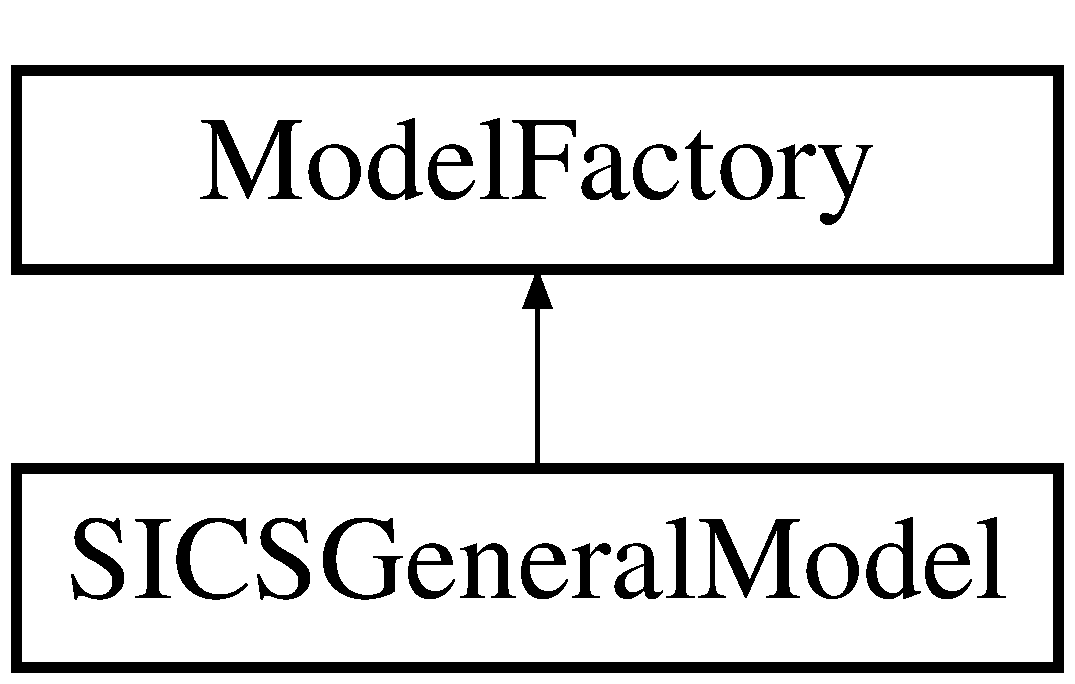
\includegraphics[height=2.000000cm]{classModelFactory}
\end{center}
\end{figure}
\subsection*{Public Member Functions}
\begin{DoxyCompactItemize}
\item 
\hyperlink{classModelFactory_aaf674444b913a74a2e1ee838cb6a9330}{Model\+Factory} ()
\item 
virtual \hyperlink{classParameterModel}{Parameter\+Model} $\ast$ \hyperlink{classModelFactory_adfa2a321dba41b9ba05e7805b9bfac2b}{create\+Parameter\+Model} ()=0
\item 
virtual \hyperlink{classItemModel}{Item\+Model} $\ast$ \hyperlink{classModelFactory_ab13ed21aabab9b4ba77173d0117a7cec}{create\+Item\+Model} ()=0
\item 
virtual \hyperlink{classDimensionModel}{Dimension\+Model} $\ast$ \hyperlink{classModelFactory_ae57ccc96f948d4df70cebc587ed0390b}{create\+Dimension\+Model} ()=0
\item 
virtual \hyperlink{classModelFactory_a4b3fc23369f942ad7f772aec8a76f9b7}{$\sim$\+Model\+Factory} ()
\end{DoxyCompactItemize}


\subsection{Detailed Description}


Definition at line 15 of file Model\+Factory.\+h.



\subsection{Constructor \& Destructor Documentation}
\hypertarget{classModelFactory_aaf674444b913a74a2e1ee838cb6a9330}{}\index{Model\+Factory@{Model\+Factory}!Model\+Factory@{Model\+Factory}}
\index{Model\+Factory@{Model\+Factory}!Model\+Factory@{Model\+Factory}}
\subsubsection[{Model\+Factory}]{\setlength{\rightskip}{0pt plus 5cm}Model\+Factory\+::\+Model\+Factory (
\begin{DoxyParamCaption}
{}
\end{DoxyParamCaption}
)}\label{classModelFactory_aaf674444b913a74a2e1ee838cb6a9330}


Definition at line 10 of file Model\+Factory.\+cpp.

\hypertarget{classModelFactory_a4b3fc23369f942ad7f772aec8a76f9b7}{}\index{Model\+Factory@{Model\+Factory}!````~Model\+Factory@{$\sim$\+Model\+Factory}}
\index{````~Model\+Factory@{$\sim$\+Model\+Factory}!Model\+Factory@{Model\+Factory}}
\subsubsection[{$\sim$\+Model\+Factory}]{\setlength{\rightskip}{0pt plus 5cm}Model\+Factory\+::$\sim$\+Model\+Factory (
\begin{DoxyParamCaption}
{}
\end{DoxyParamCaption}
)\hspace{0.3cm}{\ttfamily [virtual]}}\label{classModelFactory_a4b3fc23369f942ad7f772aec8a76f9b7}


Definition at line 15 of file Model\+Factory.\+cpp.



\subsection{Member Function Documentation}
\hypertarget{classModelFactory_ae57ccc96f948d4df70cebc587ed0390b}{}\index{Model\+Factory@{Model\+Factory}!create\+Dimension\+Model@{create\+Dimension\+Model}}
\index{create\+Dimension\+Model@{create\+Dimension\+Model}!Model\+Factory@{Model\+Factory}}
\subsubsection[{create\+Dimension\+Model}]{\setlength{\rightskip}{0pt plus 5cm}virtual {\bf Dimension\+Model}$\ast$ Model\+Factory\+::create\+Dimension\+Model (
\begin{DoxyParamCaption}
{}
\end{DoxyParamCaption}
)\hspace{0.3cm}{\ttfamily [pure virtual]}}\label{classModelFactory_ae57ccc96f948d4df70cebc587ed0390b}


Implemented in \hyperlink{classSICSGeneralModel_a35ec6c2939eba08e663a7c0b99d796a2}{S\+I\+C\+S\+General\+Model}.



Referenced by Model\+::set\+Model().

\hypertarget{classModelFactory_ab13ed21aabab9b4ba77173d0117a7cec}{}\index{Model\+Factory@{Model\+Factory}!create\+Item\+Model@{create\+Item\+Model}}
\index{create\+Item\+Model@{create\+Item\+Model}!Model\+Factory@{Model\+Factory}}
\subsubsection[{create\+Item\+Model}]{\setlength{\rightskip}{0pt plus 5cm}virtual {\bf Item\+Model}$\ast$ Model\+Factory\+::create\+Item\+Model (
\begin{DoxyParamCaption}
{}
\end{DoxyParamCaption}
)\hspace{0.3cm}{\ttfamily [pure virtual]}}\label{classModelFactory_ab13ed21aabab9b4ba77173d0117a7cec}


Implemented in \hyperlink{classSICSGeneralModel_ae6d6f2faf2b10bc67114be9d742d354e}{S\+I\+C\+S\+General\+Model}.



Referenced by Model\+::set\+Model().

\hypertarget{classModelFactory_adfa2a321dba41b9ba05e7805b9bfac2b}{}\index{Model\+Factory@{Model\+Factory}!create\+Parameter\+Model@{create\+Parameter\+Model}}
\index{create\+Parameter\+Model@{create\+Parameter\+Model}!Model\+Factory@{Model\+Factory}}
\subsubsection[{create\+Parameter\+Model}]{\setlength{\rightskip}{0pt plus 5cm}virtual {\bf Parameter\+Model}$\ast$ Model\+Factory\+::create\+Parameter\+Model (
\begin{DoxyParamCaption}
{}
\end{DoxyParamCaption}
)\hspace{0.3cm}{\ttfamily [pure virtual]}}\label{classModelFactory_adfa2a321dba41b9ba05e7805b9bfac2b}


Implemented in \hyperlink{classSICSGeneralModel_ac494be453a5c9213bfa1a959b1c985f1}{S\+I\+C\+S\+General\+Model}.



Referenced by Model\+::set\+Model().



The documentation for this class was generated from the following files\+:\begin{DoxyCompactItemize}
\item 
src/model/\hyperlink{ModelFactory_8h}{Model\+Factory.\+h}\item 
src/model/\hyperlink{ModelFactory_8cpp}{Model\+Factory.\+cpp}\end{DoxyCompactItemize}

\hypertarget{classMultidimensionalModel}{}\section{Multidimensional\+Model Class Reference}
\label{classMultidimensionalModel}\index{Multidimensional\+Model@{Multidimensional\+Model}}


{\ttfamily \#include $<$Multidimensional\+Model.\+h$>$}

Inheritance diagram for Multidimensional\+Model\+:\begin{figure}[H]
\begin{center}
\leavevmode
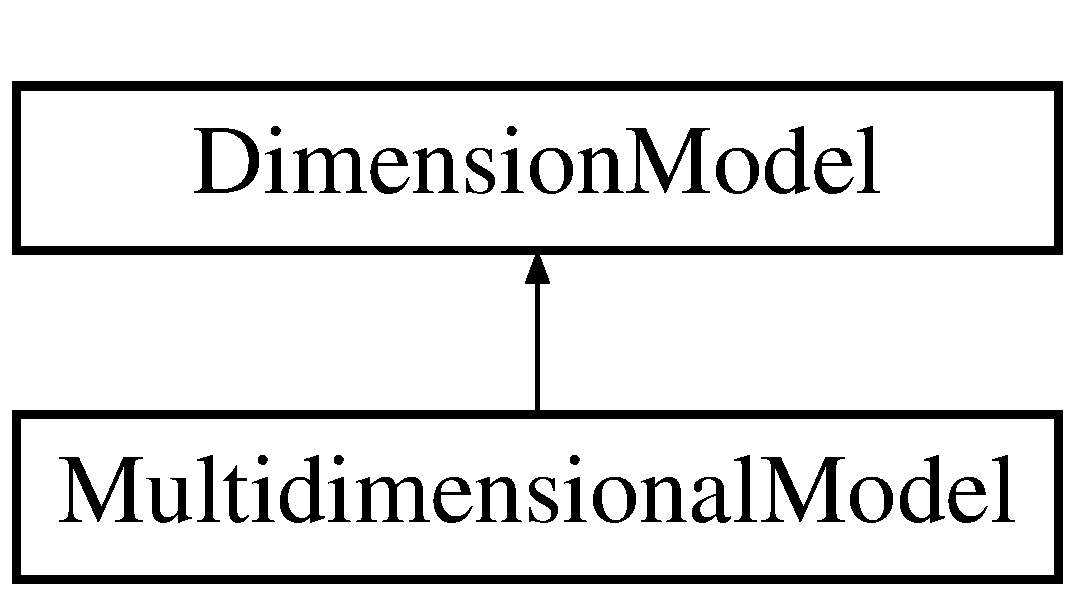
\includegraphics[height=2.000000cm]{classMultidimensionalModel}
\end{center}
\end{figure}
\subsection*{Public Member Functions}
\begin{DoxyCompactItemize}
\item 
\hyperlink{classMultidimensionalModel_ab03d019127c672972165bef2495b603f}{Multidimensional\+Model} ()
\item 
int \hyperlink{classMultidimensionalModel_ad76fe466abfab3c05bb86519440d0302}{get\+Num\+Dimensions} ()
\item 
vector$<$ int $>$ \hyperlink{classMultidimensionalModel_a6834137ae4a9d43cd73cf31025258059}{get\+Dim\+Vector} ()
\item 
\hyperlink{classLatentTraitSet}{Latent\+Trait\+Set} $\ast$ \hyperlink{classMultidimensionalModel_a94d8dcb1f23f8fa8223ef7cc2d7f860d}{get\+Latent\+Trait\+Set} () const 
\item 
void \hyperlink{classMultidimensionalModel_a367cc1d66122b0f56293271a0ffd4859}{set\+Latent\+Trait\+Set} (\hyperlink{classLatentTraitSet}{Latent\+Trait\+Set} $\ast$\hyperlink{classDimensionModel_af202cd5a44ee99d865674c6e26d770c8}{latent\+Trait\+Set})
\item 
virtual \hyperlink{classMultidimensionalModel_ab5734ccfd3223dbeb8ef0ac1d9c334f2}{$\sim$\+Multidimensional\+Model} ()
\end{DoxyCompactItemize}
\subsection*{Additional Inherited Members}


\subsection{Detailed Description}


Definition at line 17 of file Multidimensional\+Model.\+h.



\subsection{Constructor \& Destructor Documentation}
\hypertarget{classMultidimensionalModel_ab03d019127c672972165bef2495b603f}{}\index{Multidimensional\+Model@{Multidimensional\+Model}!Multidimensional\+Model@{Multidimensional\+Model}}
\index{Multidimensional\+Model@{Multidimensional\+Model}!Multidimensional\+Model@{Multidimensional\+Model}}
\subsubsection[{Multidimensional\+Model}]{\setlength{\rightskip}{0pt plus 5cm}Multidimensional\+Model\+::\+Multidimensional\+Model (
\begin{DoxyParamCaption}
{}
\end{DoxyParamCaption}
)}\label{classMultidimensionalModel_ab03d019127c672972165bef2495b603f}


Definition at line 10 of file Multidimensional\+Model.\+cpp.

\hypertarget{classMultidimensionalModel_ab5734ccfd3223dbeb8ef0ac1d9c334f2}{}\index{Multidimensional\+Model@{Multidimensional\+Model}!````~Multidimensional\+Model@{$\sim$\+Multidimensional\+Model}}
\index{````~Multidimensional\+Model@{$\sim$\+Multidimensional\+Model}!Multidimensional\+Model@{Multidimensional\+Model}}
\subsubsection[{$\sim$\+Multidimensional\+Model}]{\setlength{\rightskip}{0pt plus 5cm}Multidimensional\+Model\+::$\sim$\+Multidimensional\+Model (
\begin{DoxyParamCaption}
{}
\end{DoxyParamCaption}
)\hspace{0.3cm}{\ttfamily [virtual]}}\label{classMultidimensionalModel_ab5734ccfd3223dbeb8ef0ac1d9c334f2}


Definition at line 18 of file Multidimensional\+Model.\+cpp.



\subsection{Member Function Documentation}
\hypertarget{classMultidimensionalModel_a6834137ae4a9d43cd73cf31025258059}{}\index{Multidimensional\+Model@{Multidimensional\+Model}!get\+Dim\+Vector@{get\+Dim\+Vector}}
\index{get\+Dim\+Vector@{get\+Dim\+Vector}!Multidimensional\+Model@{Multidimensional\+Model}}
\subsubsection[{get\+Dim\+Vector}]{\setlength{\rightskip}{0pt plus 5cm}vector$<$ int $>$ Multidimensional\+Model\+::get\+Dim\+Vector (
\begin{DoxyParamCaption}
{}
\end{DoxyParamCaption}
)\hspace{0.3cm}{\ttfamily [virtual]}}\label{classMultidimensionalModel_a6834137ae4a9d43cd73cf31025258059}


Implements \hyperlink{classDimensionModel_a0aab2664f71949ac52d654730840056b}{Dimension\+Model}.



Definition at line 15 of file Multidimensional\+Model.\+cpp.

\hypertarget{classMultidimensionalModel_a94d8dcb1f23f8fa8223ef7cc2d7f860d}{}\index{Multidimensional\+Model@{Multidimensional\+Model}!get\+Latent\+Trait\+Set@{get\+Latent\+Trait\+Set}}
\index{get\+Latent\+Trait\+Set@{get\+Latent\+Trait\+Set}!Multidimensional\+Model@{Multidimensional\+Model}}
\subsubsection[{get\+Latent\+Trait\+Set}]{\setlength{\rightskip}{0pt plus 5cm}{\bf Latent\+Trait\+Set} $\ast$ Multidimensional\+Model\+::get\+Latent\+Trait\+Set (
\begin{DoxyParamCaption}
{}
\end{DoxyParamCaption}
) const\hspace{0.3cm}{\ttfamily [virtual]}}\label{classMultidimensionalModel_a94d8dcb1f23f8fa8223ef7cc2d7f860d}


Implements \hyperlink{classDimensionModel_a37d2d9ab998a4e65628571e6144311f6}{Dimension\+Model}.



Definition at line 22 of file Multidimensional\+Model.\+cpp.



References Dimension\+Model\+::latent\+Trait\+Set.

\hypertarget{classMultidimensionalModel_ad76fe466abfab3c05bb86519440d0302}{}\index{Multidimensional\+Model@{Multidimensional\+Model}!get\+Num\+Dimensions@{get\+Num\+Dimensions}}
\index{get\+Num\+Dimensions@{get\+Num\+Dimensions}!Multidimensional\+Model@{Multidimensional\+Model}}
\subsubsection[{get\+Num\+Dimensions}]{\setlength{\rightskip}{0pt plus 5cm}int Multidimensional\+Model\+::get\+Num\+Dimensions (
\begin{DoxyParamCaption}
{}
\end{DoxyParamCaption}
)\hspace{0.3cm}{\ttfamily [virtual]}}\label{classMultidimensionalModel_ad76fe466abfab3c05bb86519440d0302}


Implements \hyperlink{classDimensionModel_aaf16c9215f4a7d08d67bd844adfcc62a}{Dimension\+Model}.



Definition at line 31 of file Multidimensional\+Model.\+cpp.

\hypertarget{classMultidimensionalModel_a367cc1d66122b0f56293271a0ffd4859}{}\index{Multidimensional\+Model@{Multidimensional\+Model}!set\+Latent\+Trait\+Set@{set\+Latent\+Trait\+Set}}
\index{set\+Latent\+Trait\+Set@{set\+Latent\+Trait\+Set}!Multidimensional\+Model@{Multidimensional\+Model}}
\subsubsection[{set\+Latent\+Trait\+Set}]{\setlength{\rightskip}{0pt plus 5cm}void Multidimensional\+Model\+::set\+Latent\+Trait\+Set (
\begin{DoxyParamCaption}
\item[{{\bf Latent\+Trait\+Set} $\ast$}]{latent\+Trait\+Set}
\end{DoxyParamCaption}
)\hspace{0.3cm}{\ttfamily [virtual]}}\label{classMultidimensionalModel_a367cc1d66122b0f56293271a0ffd4859}


Implements \hyperlink{classDimensionModel_aed42259f6cd663cbd1df07d18d4b1e07}{Dimension\+Model}.



Definition at line 26 of file Multidimensional\+Model.\+cpp.



References Dimension\+Model\+::latent\+Trait\+Set.



The documentation for this class was generated from the following files\+:\begin{DoxyCompactItemize}
\item 
src/model/dimension/\hyperlink{MultidimensionalModel_8h}{Multidimensional\+Model.\+h}\item 
src/model/dimension/\hyperlink{MultidimensionalModel_8cpp}{Multidimensional\+Model.\+cpp}\end{DoxyCompactItemize}

\hypertarget{classMultiUniDimModel}{}\section{Multi\+Uni\+Dim\+Model Class Reference}
\label{classMultiUniDimModel}\index{Multi\+Uni\+Dim\+Model@{Multi\+Uni\+Dim\+Model}}


{\ttfamily \#include $<$Multi\+Uni\+Dim\+Model.\+h$>$}

Inheritance diagram for Multi\+Uni\+Dim\+Model\+:\begin{figure}[H]
\begin{center}
\leavevmode
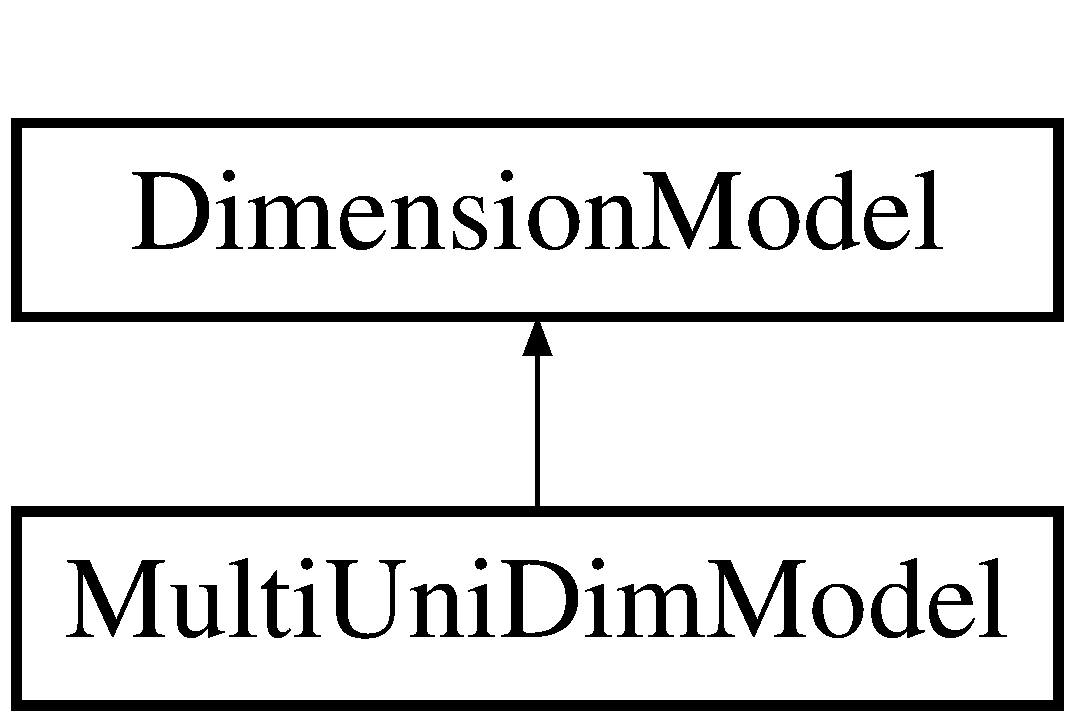
\includegraphics[height=2.000000cm]{classMultiUniDimModel}
\end{center}
\end{figure}
\subsection*{Public Member Functions}
\begin{DoxyCompactItemize}
\item 
\hyperlink{classMultiUniDimModel_a9c267d062e0d311ab39f27144827de05}{Multi\+Uni\+Dim\+Model} ()
\item 
int \hyperlink{classMultiUniDimModel_a6789b80610d6db4985dc51020313b158}{get\+Num\+Dimensions} ()
\item 
vector$<$ int $>$ \hyperlink{classMultiUniDimModel_a1e92f67a87f5b406f0382e9cb240f889}{get\+Dim\+Vector} ()
\item 
\hyperlink{classLatentTraitSet}{Latent\+Trait\+Set} $\ast$ \hyperlink{classMultiUniDimModel_aa3b9917e93a9498f5eb95c74a2335797}{get\+Latent\+Trait\+Set} () const 
\item 
void \hyperlink{classMultiUniDimModel_ac13d9476e8687888d1a290704561e704}{set\+Latent\+Trait\+Set} (\hyperlink{classLatentTraitSet}{Latent\+Trait\+Set} $\ast$\hyperlink{classDimensionModel_af202cd5a44ee99d865674c6e26d770c8}{latent\+Trait\+Set})
\item 
virtual \hyperlink{classMultiUniDimModel_ab0299e7f4747366d8ef47d3015970cd2}{$\sim$\+Multi\+Uni\+Dim\+Model} ()
\end{DoxyCompactItemize}
\subsection*{Additional Inherited Members}


\subsection{Detailed Description}


Definition at line 13 of file Multi\+Uni\+Dim\+Model.\+h.



\subsection{Constructor \& Destructor Documentation}
\hypertarget{classMultiUniDimModel_a9c267d062e0d311ab39f27144827de05}{}\index{Multi\+Uni\+Dim\+Model@{Multi\+Uni\+Dim\+Model}!Multi\+Uni\+Dim\+Model@{Multi\+Uni\+Dim\+Model}}
\index{Multi\+Uni\+Dim\+Model@{Multi\+Uni\+Dim\+Model}!Multi\+Uni\+Dim\+Model@{Multi\+Uni\+Dim\+Model}}
\subsubsection[{Multi\+Uni\+Dim\+Model}]{\setlength{\rightskip}{0pt plus 5cm}Multi\+Uni\+Dim\+Model\+::\+Multi\+Uni\+Dim\+Model (
\begin{DoxyParamCaption}
{}
\end{DoxyParamCaption}
)}\label{classMultiUniDimModel_a9c267d062e0d311ab39f27144827de05}


Definition at line 10 of file Multi\+Uni\+Dim\+Model.\+cpp.

\hypertarget{classMultiUniDimModel_ab0299e7f4747366d8ef47d3015970cd2}{}\index{Multi\+Uni\+Dim\+Model@{Multi\+Uni\+Dim\+Model}!````~Multi\+Uni\+Dim\+Model@{$\sim$\+Multi\+Uni\+Dim\+Model}}
\index{````~Multi\+Uni\+Dim\+Model@{$\sim$\+Multi\+Uni\+Dim\+Model}!Multi\+Uni\+Dim\+Model@{Multi\+Uni\+Dim\+Model}}
\subsubsection[{$\sim$\+Multi\+Uni\+Dim\+Model}]{\setlength{\rightskip}{0pt plus 5cm}Multi\+Uni\+Dim\+Model\+::$\sim$\+Multi\+Uni\+Dim\+Model (
\begin{DoxyParamCaption}
{}
\end{DoxyParamCaption}
)\hspace{0.3cm}{\ttfamily [virtual]}}\label{classMultiUniDimModel_ab0299e7f4747366d8ef47d3015970cd2}


Definition at line 29 of file Multi\+Uni\+Dim\+Model.\+cpp.



\subsection{Member Function Documentation}
\hypertarget{classMultiUniDimModel_a1e92f67a87f5b406f0382e9cb240f889}{}\index{Multi\+Uni\+Dim\+Model@{Multi\+Uni\+Dim\+Model}!get\+Dim\+Vector@{get\+Dim\+Vector}}
\index{get\+Dim\+Vector@{get\+Dim\+Vector}!Multi\+Uni\+Dim\+Model@{Multi\+Uni\+Dim\+Model}}
\subsubsection[{get\+Dim\+Vector}]{\setlength{\rightskip}{0pt plus 5cm}vector$<$ int $>$ Multi\+Uni\+Dim\+Model\+::get\+Dim\+Vector (
\begin{DoxyParamCaption}
{}
\end{DoxyParamCaption}
)\hspace{0.3cm}{\ttfamily [virtual]}}\label{classMultiUniDimModel_a1e92f67a87f5b406f0382e9cb240f889}


Implements \hyperlink{classDimensionModel_a0aab2664f71949ac52d654730840056b}{Dimension\+Model}.



Definition at line 18 of file Multi\+Uni\+Dim\+Model.\+cpp.

\hypertarget{classMultiUniDimModel_aa3b9917e93a9498f5eb95c74a2335797}{}\index{Multi\+Uni\+Dim\+Model@{Multi\+Uni\+Dim\+Model}!get\+Latent\+Trait\+Set@{get\+Latent\+Trait\+Set}}
\index{get\+Latent\+Trait\+Set@{get\+Latent\+Trait\+Set}!Multi\+Uni\+Dim\+Model@{Multi\+Uni\+Dim\+Model}}
\subsubsection[{get\+Latent\+Trait\+Set}]{\setlength{\rightskip}{0pt plus 5cm}{\bf Latent\+Trait\+Set} $\ast$ Multi\+Uni\+Dim\+Model\+::get\+Latent\+Trait\+Set (
\begin{DoxyParamCaption}
{}
\end{DoxyParamCaption}
) const\hspace{0.3cm}{\ttfamily [virtual]}}\label{classMultiUniDimModel_aa3b9917e93a9498f5eb95c74a2335797}


Implements \hyperlink{classDimensionModel_a37d2d9ab998a4e65628571e6144311f6}{Dimension\+Model}.



Definition at line 21 of file Multi\+Uni\+Dim\+Model.\+cpp.



References Dimension\+Model\+::latent\+Trait\+Set.

\hypertarget{classMultiUniDimModel_a6789b80610d6db4985dc51020313b158}{}\index{Multi\+Uni\+Dim\+Model@{Multi\+Uni\+Dim\+Model}!get\+Num\+Dimensions@{get\+Num\+Dimensions}}
\index{get\+Num\+Dimensions@{get\+Num\+Dimensions}!Multi\+Uni\+Dim\+Model@{Multi\+Uni\+Dim\+Model}}
\subsubsection[{get\+Num\+Dimensions}]{\setlength{\rightskip}{0pt plus 5cm}int Multi\+Uni\+Dim\+Model\+::get\+Num\+Dimensions (
\begin{DoxyParamCaption}
{}
\end{DoxyParamCaption}
)\hspace{0.3cm}{\ttfamily [virtual]}}\label{classMultiUniDimModel_a6789b80610d6db4985dc51020313b158}


Implements \hyperlink{classDimensionModel_aaf16c9215f4a7d08d67bd844adfcc62a}{Dimension\+Model}.



Definition at line 15 of file Multi\+Uni\+Dim\+Model.\+cpp.

\hypertarget{classMultiUniDimModel_ac13d9476e8687888d1a290704561e704}{}\index{Multi\+Uni\+Dim\+Model@{Multi\+Uni\+Dim\+Model}!set\+Latent\+Trait\+Set@{set\+Latent\+Trait\+Set}}
\index{set\+Latent\+Trait\+Set@{set\+Latent\+Trait\+Set}!Multi\+Uni\+Dim\+Model@{Multi\+Uni\+Dim\+Model}}
\subsubsection[{set\+Latent\+Trait\+Set}]{\setlength{\rightskip}{0pt plus 5cm}void Multi\+Uni\+Dim\+Model\+::set\+Latent\+Trait\+Set (
\begin{DoxyParamCaption}
\item[{{\bf Latent\+Trait\+Set} $\ast$}]{latent\+Trait\+Set}
\end{DoxyParamCaption}
)\hspace{0.3cm}{\ttfamily [virtual]}}\label{classMultiUniDimModel_ac13d9476e8687888d1a290704561e704}


Implements \hyperlink{classDimensionModel_aed42259f6cd663cbd1df07d18d4b1e07}{Dimension\+Model}.



Definition at line 25 of file Multi\+Uni\+Dim\+Model.\+cpp.



References Dimension\+Model\+::latent\+Trait\+Set.



The documentation for this class was generated from the following files\+:\begin{DoxyCompactItemize}
\item 
src/model/dimension/\hyperlink{MultiUniDimModel_8h}{Multi\+Uni\+Dim\+Model.\+h}\item 
src/model/dimension/\hyperlink{MultiUniDimModel_8cpp}{Multi\+Uni\+Dim\+Model.\+cpp}\end{DoxyCompactItemize}

\hypertarget{classOptimizer}{}\section{Optimizer Class Reference}
\label{classOptimizer}\index{Optimizer@{Optimizer}}


Wrapper for the other optimizers, take general functions for the function to optimize, the vector gradient function and the matrix hessian function The parameters are \+: double $\ast$ args (Arguments over which the function optimizes) double $\ast$ pars (Arguments in whose the function depends but are not optimized) int nargs Number of arguments int npars Number of parameters double $\ast$ return (Return of the function is put in this array.)  




{\ttfamily \#include $<$Optimizer.\+h$>$}

\subsection*{Public Member Functions}
\begin{DoxyCompactItemize}
\item 
void \hyperlink{classOptimizer_ab3c54cfddcd5e97c1dae4cc6bd4e4e92}{search\+Optimal} (double($\ast$function\+Ptr)(double $\ast$, double $\ast$, int, int), void($\ast$gradient\+Ptr)(double $\ast$, double $\ast$, int, int, double $\ast$), void($\ast$Hessian\+Ptr)(double $\ast$, double $\ast$, int, int, double $\ast$), double $\ast$args, double $\ast$pars, int nargs, int npars)
\item 
\hyperlink{classOptimizer_ab01202385afea2f09afbd73227736a17}{$\sim$\+Optimizer} ()
\end{DoxyCompactItemize}


\subsection{Detailed Description}
Wrapper for the other optimizers, take general functions for the function to optimize, the vector gradient function and the matrix hessian function The parameters are \+: double $\ast$ args (Arguments over which the function optimizes) double $\ast$ pars (Arguments in whose the function depends but are not optimized) int nargs Number of arguments int npars Number of parameters double $\ast$ return (Return of the function is put in this array.) 

Definition at line 24 of file Optimizer.\+h.



\subsection{Constructor \& Destructor Documentation}
\hypertarget{classOptimizer_ab01202385afea2f09afbd73227736a17}{}\index{Optimizer@{Optimizer}!````~Optimizer@{$\sim$\+Optimizer}}
\index{````~Optimizer@{$\sim$\+Optimizer}!Optimizer@{Optimizer}}
\subsubsection[{$\sim$\+Optimizer}]{\setlength{\rightskip}{0pt plus 5cm}Optimizer\+::$\sim$\+Optimizer (
\begin{DoxyParamCaption}
{}
\end{DoxyParamCaption}
)}\label{classOptimizer_ab01202385afea2f09afbd73227736a17}


Definition at line 12 of file Optimizer.\+cpp.



\subsection{Member Function Documentation}
\hypertarget{classOptimizer_ab3c54cfddcd5e97c1dae4cc6bd4e4e92}{}\index{Optimizer@{Optimizer}!search\+Optimal@{search\+Optimal}}
\index{search\+Optimal@{search\+Optimal}!Optimizer@{Optimizer}}
\subsubsection[{search\+Optimal}]{\setlength{\rightskip}{0pt plus 5cm}void Optimizer\+::search\+Optimal (
\begin{DoxyParamCaption}
\item[{double($\ast$)(double $\ast$, double $\ast$, int, int)}]{function\+Ptr, }
\item[{void($\ast$)(double $\ast$, double $\ast$, int, int, double $\ast$)}]{gradient\+Ptr, }
\item[{void($\ast$)(double $\ast$, double $\ast$, int, int, double $\ast$)}]{Hessian\+Ptr, }
\item[{double $\ast$}]{args, }
\item[{double $\ast$}]{pars, }
\item[{int}]{nargs, }
\item[{int}]{npars}
\end{DoxyParamCaption}
)}\label{classOptimizer_ab3c54cfddcd5e97c1dae4cc6bd4e4e92}


Definition at line 3 of file Optimizer.\+cpp.



Referenced by rosenbrock\+Test(), and E\+M\+Estimation\+::step\+M().



The documentation for this class was generated from the following files\+:\begin{DoxyCompactItemize}
\item 
src/optimizer/\hyperlink{Optimizer_8h}{Optimizer.\+h}\item 
src/optimizer/\hyperlink{Optimizer_8cpp}{Optimizer.\+cpp}\end{DoxyCompactItemize}

\hypertarget{classOutput}{}\section{Output Class Reference}
\label{classOutput}\index{Output@{Output}}


Skeleton for the output class T\+O\+D\+O \+: C\+S\+V output T\+O\+D\+O \+: J\+S\+O\+N online output T\+O\+D\+O \+: Te\+X output for reports.  




{\ttfamily \#include $<$Output.\+h$>$}

\subsection*{Public Member Functions}
\begin{DoxyCompactItemize}
\item 
\hyperlink{classOutput_a428c663520336477a12f1a33504eb067}{Output} ()
\item 
virtual \hyperlink{classOutput_a61d0840daf98bea49e4dc471f235eeab}{$\sim$\+Output} ()
\end{DoxyCompactItemize}


\subsection{Detailed Description}
Skeleton for the output class T\+O\+D\+O \+: C\+S\+V output T\+O\+D\+O \+: J\+S\+O\+N online output T\+O\+D\+O \+: Te\+X output for reports. 

Definition at line 18 of file Output.\+h.



\subsection{Constructor \& Destructor Documentation}
\hypertarget{classOutput_a428c663520336477a12f1a33504eb067}{}\index{Output@{Output}!Output@{Output}}
\index{Output@{Output}!Output@{Output}}
\subsubsection[{Output}]{\setlength{\rightskip}{0pt plus 5cm}Output\+::\+Output (
\begin{DoxyParamCaption}
{}
\end{DoxyParamCaption}
)}\label{classOutput_a428c663520336477a12f1a33504eb067}


Definition at line 10 of file Output.\+cpp.

\hypertarget{classOutput_a61d0840daf98bea49e4dc471f235eeab}{}\index{Output@{Output}!````~Output@{$\sim$\+Output}}
\index{````~Output@{$\sim$\+Output}!Output@{Output}}
\subsubsection[{$\sim$\+Output}]{\setlength{\rightskip}{0pt plus 5cm}Output\+::$\sim$\+Output (
\begin{DoxyParamCaption}
{}
\end{DoxyParamCaption}
)\hspace{0.3cm}{\ttfamily [virtual]}}\label{classOutput_a61d0840daf98bea49e4dc471f235eeab}


Definition at line 15 of file Output.\+cpp.



The documentation for this class was generated from the following files\+:\begin{DoxyCompactItemize}
\item 
src/output/\hyperlink{Output_8h}{Output.\+h}\item 
src/output/\hyperlink{Output_8cpp}{Output.\+cpp}\end{DoxyCompactItemize}

\hypertarget{classParameterModel}{}\section{Parameter\+Model Class Reference}
\label{classParameterModel}\index{Parameter\+Model@{Parameter\+Model}}


{\ttfamily \#include $<$Parameter\+Model.\+h$>$}

Inheritance diagram for Parameter\+Model\+:\begin{figure}[H]
\begin{center}
\leavevmode
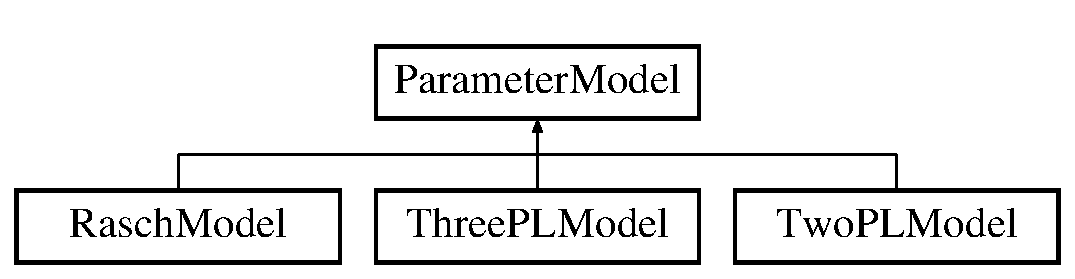
\includegraphics[height=2.000000cm]{classParameterModel}
\end{center}
\end{figure}
\subsection*{Public Member Functions}
\begin{DoxyCompactItemize}
\item 
virtual void \hyperlink{classParameterModel_a2f02140d0b27796ccdaf9cadbccb2e2f}{build\+Parameter\+Set} (\hyperlink{classItemModel}{Item\+Model} $\ast$, \hyperlink{classDimensionModel}{Dimension\+Model} $\ast$)=0
\item 
virtual void \hyperlink{classParameterModel_a13249755ab9078be82262896beff5c17}{success\+Probability} (\hyperlink{classDimensionModel}{Dimension\+Model} $\ast$)=0
\item 
virtual map$<$ \hyperlink{ParameterModel_8h_a04ed5b8f1f3adf7af1d5092fae847e90}{Parameter}, \hyperlink{singletonMatrix}{Matrix}$<$ double $>$ $\ast$ $>$ \hyperlink{classParameterModel_aa4e52819318c9dcc9087a36d1a940c0b}{get\+Parameter\+Set} ()=0
\item 
virtual void \hyperlink{classParameterModel_aa13375bcd79d7c1afbde0a8f179f38cb}{set\+Parameter\+Set} (map$<$ \hyperlink{ParameterModel_8h_a04ed5b8f1f3adf7af1d5092fae847e90}{Parameter}, \hyperlink{singletonMatrix}{Matrix}$<$ double $>$ $\ast$ $>$ \hyperlink{classParameterModel_a0b5dafa68a235673a229863aa66ae97d}{parameter\+Set})=0
\item 
virtual double \hyperlink{classParameterModel_ac706c102c88bb20f5d47e61eb8d5dc7e}{get\+Probability} (int, int)=0
\item 
virtual \hyperlink{classParameterModel_a55dd5151867a9359aa27a430432f6889}{$\sim$\+Parameter\+Model} ()
\end{DoxyCompactItemize}
\subsection*{Public Attributes}
\begin{DoxyCompactItemize}
\item 
\hyperlink{singletonMatrix}{Matrix}$<$ double $>$ $\ast$ \hyperlink{classParameterModel_a4be41bcd6697769578a729e2279014eb}{probability\+Matrix}
\end{DoxyCompactItemize}
\subsection*{Protected Attributes}
\begin{DoxyCompactItemize}
\item 
map$<$ \hyperlink{ParameterModel_8h_a04ed5b8f1f3adf7af1d5092fae847e90}{Parameter}, \hyperlink{singletonMatrix}{Matrix}$<$ double $>$ $\ast$ $>$ \hyperlink{classParameterModel_a0b5dafa68a235673a229863aa66ae97d}{parameter\+Set}
\end{DoxyCompactItemize}


\subsection{Detailed Description}


Definition at line 21 of file Parameter\+Model.\+h.



\subsection{Constructor \& Destructor Documentation}
\hypertarget{classParameterModel_a55dd5151867a9359aa27a430432f6889}{}\index{Parameter\+Model@{Parameter\+Model}!````~Parameter\+Model@{$\sim$\+Parameter\+Model}}
\index{````~Parameter\+Model@{$\sim$\+Parameter\+Model}!Parameter\+Model@{Parameter\+Model}}
\subsubsection[{$\sim$\+Parameter\+Model}]{\setlength{\rightskip}{0pt plus 5cm}Parameter\+Model\+::$\sim$\+Parameter\+Model (
\begin{DoxyParamCaption}
{}
\end{DoxyParamCaption}
)\hspace{0.3cm}{\ttfamily [virtual]}}\label{classParameterModel_a55dd5151867a9359aa27a430432f6889}


Definition at line 10 of file Parameter\+Model.\+cpp.



\subsection{Member Function Documentation}
\hypertarget{classParameterModel_a2f02140d0b27796ccdaf9cadbccb2e2f}{}\index{Parameter\+Model@{Parameter\+Model}!build\+Parameter\+Set@{build\+Parameter\+Set}}
\index{build\+Parameter\+Set@{build\+Parameter\+Set}!Parameter\+Model@{Parameter\+Model}}
\subsubsection[{build\+Parameter\+Set}]{\setlength{\rightskip}{0pt plus 5cm}virtual void Parameter\+Model\+::build\+Parameter\+Set (
\begin{DoxyParamCaption}
\item[{{\bf Item\+Model} $\ast$}]{, }
\item[{{\bf Dimension\+Model} $\ast$}]{}
\end{DoxyParamCaption}
)\hspace{0.3cm}{\ttfamily [pure virtual]}}\label{classParameterModel_a2f02140d0b27796ccdaf9cadbccb2e2f}


Implemented in \hyperlink{classThreePLModel_a7242d2bf961e6bf167cc7ca89cf36a67}{Three\+P\+L\+Model}, \hyperlink{classRaschModel_a73b865f129db10fb7ba74495c3fce60b}{Rasch\+Model}, and \hyperlink{classTwoPLModel_aabf6941cbcad7f5a73af30725a4bcb31}{Two\+P\+L\+Model}.



Referenced by Model\+::build\+Parameter\+Set(), and one\+Run().

\hypertarget{classParameterModel_aa4e52819318c9dcc9087a36d1a940c0b}{}\index{Parameter\+Model@{Parameter\+Model}!get\+Parameter\+Set@{get\+Parameter\+Set}}
\index{get\+Parameter\+Set@{get\+Parameter\+Set}!Parameter\+Model@{Parameter\+Model}}
\subsubsection[{get\+Parameter\+Set}]{\setlength{\rightskip}{0pt plus 5cm}virtual map$<${\bf Parameter}, {\bf Matrix}$<$double$>$ $\ast$$>$ Parameter\+Model\+::get\+Parameter\+Set (
\begin{DoxyParamCaption}
{}
\end{DoxyParamCaption}
)\hspace{0.3cm}{\ttfamily [pure virtual]}}\label{classParameterModel_aa4e52819318c9dcc9087a36d1a940c0b}


Implemented in \hyperlink{classThreePLModel_ae87fb19a09c536da3fb9cbbfc443bc8e}{Three\+P\+L\+Model}, \hyperlink{classRaschModel_aee54609e4db0cb065dc1761e787e8ba9}{Rasch\+Model}, and \hyperlink{classTwoPLModel_a954cc66bfa5e79838130c09ff2d96edf}{Two\+P\+L\+Model}.



Referenced by E\+M\+Estimation\+::estimate(), E\+M\+Estimation\+::set\+Initial\+Values(), E\+M\+Estimation\+::step\+E(), and E\+M\+Estimation\+::step\+M().

\hypertarget{classParameterModel_ac706c102c88bb20f5d47e61eb8d5dc7e}{}\index{Parameter\+Model@{Parameter\+Model}!get\+Probability@{get\+Probability}}
\index{get\+Probability@{get\+Probability}!Parameter\+Model@{Parameter\+Model}}
\subsubsection[{get\+Probability}]{\setlength{\rightskip}{0pt plus 5cm}virtual double Parameter\+Model\+::get\+Probability (
\begin{DoxyParamCaption}
\item[{int}]{, }
\item[{int}]{}
\end{DoxyParamCaption}
)\hspace{0.3cm}{\ttfamily [pure virtual]}}\label{classParameterModel_ac706c102c88bb20f5d47e61eb8d5dc7e}


Implemented in \hyperlink{classThreePLModel_a36cdc7dc2e7b009a54c773de3645707b}{Three\+P\+L\+Model}, \hyperlink{classRaschModel_ae9a8edbdf6d1e5b801fb291b7035fc79}{Rasch\+Model}, and \hyperlink{classTwoPLModel_a89a707b9813ff8c8999267604cc67c62}{Two\+P\+L\+Model}.



Referenced by E\+M\+Estimation\+::step\+E().

\hypertarget{classParameterModel_aa13375bcd79d7c1afbde0a8f179f38cb}{}\index{Parameter\+Model@{Parameter\+Model}!set\+Parameter\+Set@{set\+Parameter\+Set}}
\index{set\+Parameter\+Set@{set\+Parameter\+Set}!Parameter\+Model@{Parameter\+Model}}
\subsubsection[{set\+Parameter\+Set}]{\setlength{\rightskip}{0pt plus 5cm}virtual void Parameter\+Model\+::set\+Parameter\+Set (
\begin{DoxyParamCaption}
\item[{map$<$ {\bf Parameter}, {\bf Matrix}$<$ double $>$ $\ast$ $>$}]{parameter\+Set}
\end{DoxyParamCaption}
)\hspace{0.3cm}{\ttfamily [pure virtual]}}\label{classParameterModel_aa13375bcd79d7c1afbde0a8f179f38cb}


Implemented in \hyperlink{classThreePLModel_aa049135b26ea1a9f81f23dfac6195696}{Three\+P\+L\+Model}, \hyperlink{classRaschModel_a3c4614d2536c807cea40df2301c063ca}{Rasch\+Model}, and \hyperlink{classTwoPLModel_a1a699dcb6b2890e1b2574778c2ec688e}{Two\+P\+L\+Model}.



Referenced by E\+M\+Estimation\+::set\+Initial\+Values(), and E\+M\+Estimation\+::step\+M().

\hypertarget{classParameterModel_a13249755ab9078be82262896beff5c17}{}\index{Parameter\+Model@{Parameter\+Model}!success\+Probability@{success\+Probability}}
\index{success\+Probability@{success\+Probability}!Parameter\+Model@{Parameter\+Model}}
\subsubsection[{success\+Probability}]{\setlength{\rightskip}{0pt plus 5cm}virtual void Parameter\+Model\+::success\+Probability (
\begin{DoxyParamCaption}
\item[{{\bf Dimension\+Model} $\ast$}]{}
\end{DoxyParamCaption}
)\hspace{0.3cm}{\ttfamily [pure virtual]}}\label{classParameterModel_a13249755ab9078be82262896beff5c17}


Implemented in \hyperlink{classThreePLModel_a983cdd653542d76b150c502ac88a3a0d}{Three\+P\+L\+Model}, \hyperlink{classRaschModel_a3d082fd28aa10277623dd665d2127d64}{Rasch\+Model}, and \hyperlink{classTwoPLModel_a3fb1a6228da24ce1ee7a2bedb6a2f2e7}{Two\+P\+L\+Model}.



Referenced by Model\+::success\+Probability().



\subsection{Member Data Documentation}
\hypertarget{classParameterModel_a0b5dafa68a235673a229863aa66ae97d}{}\index{Parameter\+Model@{Parameter\+Model}!parameter\+Set@{parameter\+Set}}
\index{parameter\+Set@{parameter\+Set}!Parameter\+Model@{Parameter\+Model}}
\subsubsection[{parameter\+Set}]{\setlength{\rightskip}{0pt plus 5cm}map$<${\bf Parameter}, {\bf Matrix}$<$double$>$ $\ast$ $>$ Parameter\+Model\+::parameter\+Set\hspace{0.3cm}{\ttfamily [protected]}}\label{classParameterModel_a0b5dafa68a235673a229863aa66ae97d}


Definition at line 24 of file Parameter\+Model.\+h.



Referenced by Three\+P\+L\+Model\+::build\+Parameter\+Set(), Rasch\+Model\+::get\+Parameter\+Set(), Two\+P\+L\+Model\+::get\+Parameter\+Set(), Three\+P\+L\+Model\+::get\+Parameter\+Set(), Rasch\+Model\+::set\+Parameter\+Set(), Two\+P\+L\+Model\+::set\+Parameter\+Set(), Three\+P\+L\+Model\+::set\+Parameter\+Set(), Three\+P\+L\+Model\+::success\+Probability(), Three\+P\+L\+Model\+::\+Three\+P\+L\+Model(), and Three\+P\+L\+Model\+::$\sim$\+Three\+P\+L\+Model().

\hypertarget{classParameterModel_a4be41bcd6697769578a729e2279014eb}{}\index{Parameter\+Model@{Parameter\+Model}!probability\+Matrix@{probability\+Matrix}}
\index{probability\+Matrix@{probability\+Matrix}!Parameter\+Model@{Parameter\+Model}}
\subsubsection[{probability\+Matrix}]{\setlength{\rightskip}{0pt plus 5cm}{\bf Matrix}$<$double$>$$\ast$ Parameter\+Model\+::probability\+Matrix}\label{classParameterModel_a4be41bcd6697769578a729e2279014eb}


Definition at line 26 of file Parameter\+Model.\+h.



Referenced by Three\+P\+L\+Model\+::build\+Parameter\+Set(), Three\+P\+L\+Model\+::get\+Probability(), and Three\+P\+L\+Model\+::\+Three\+P\+L\+Model().



The documentation for this class was generated from the following files\+:\begin{DoxyCompactItemize}
\item 
src/model/parameter/\hyperlink{ParameterModel_8h}{Parameter\+Model.\+h}\item 
src/model/parameter/\hyperlink{ParameterModel_8cpp}{Parameter\+Model.\+cpp}\end{DoxyCompactItemize}

\hypertarget{classPatternMatrix}{}\section{Pattern\+Matrix Class Reference}
\label{classPatternMatrix}\index{Pattern\+Matrix@{Pattern\+Matrix}}


Class for holding binary matrices in the array of patterns of bitsets form.  




{\ttfamily \#include $<$Pattern\+Matrix.\+h$>$}

Inheritance diagram for Pattern\+Matrix\+:\begin{figure}[H]
\begin{center}
\leavevmode
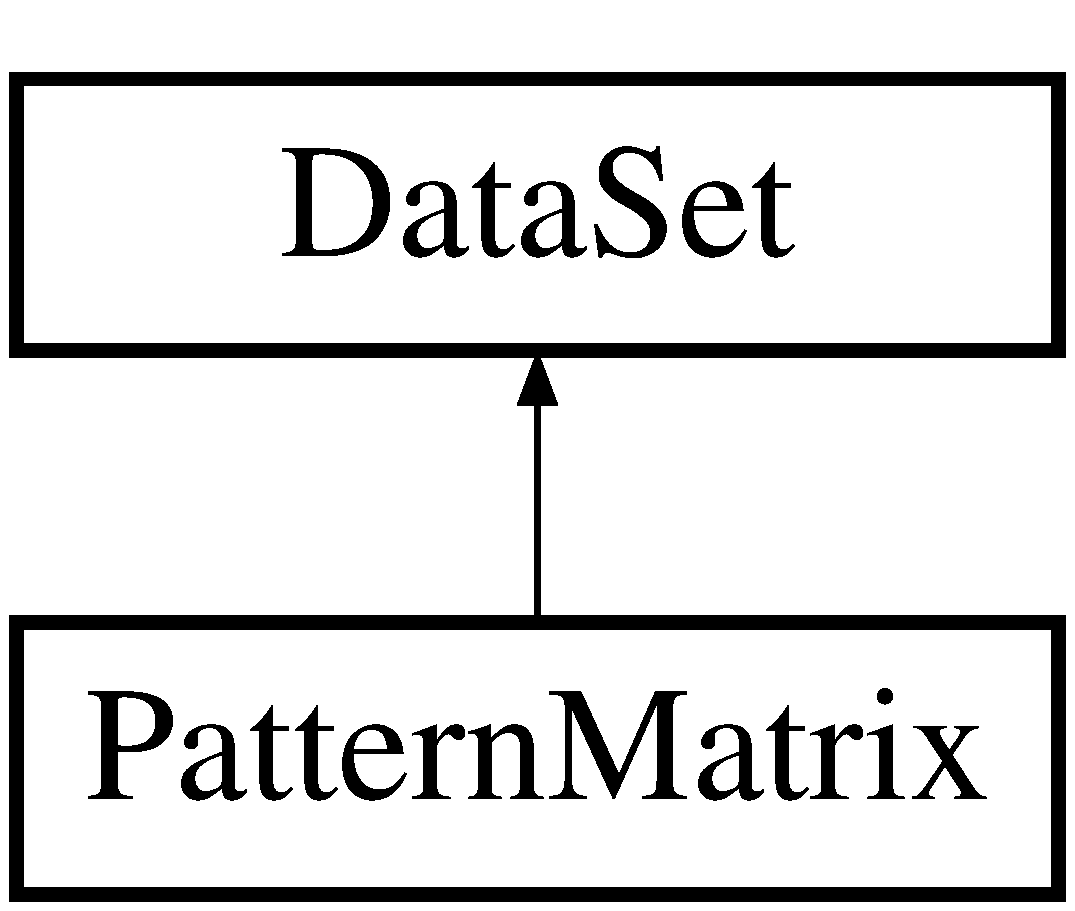
\includegraphics[height=2.000000cm]{classPatternMatrix}
\end{center}
\end{figure}
\subsection*{Public Member Functions}
\begin{DoxyCompactItemize}
\item 
\hyperlink{classPatternMatrix_aaaf6e5d86e4d5fd0bbc907f5c445f1d7}{Pattern\+Matrix} ()
\item 
void \hyperlink{classPatternMatrix_a636096859a24b38dd40623e581bcb460}{reset\+Iterator} ()
\begin{DoxyCompactList}\small\item\em use this when reading in order \end{DoxyCompactList}\item 
bool \hyperlink{classPatternMatrix_ae005cb9835142294ed5cbad3c9ab6a0f}{check\+End} ()
\item 
void \hyperlink{classPatternMatrix_a6b6ba61b62f8bfdba73531d47c64564b}{iterate} ()
\item 
void \hyperlink{classPatternMatrix_a45439edd37b28bf95db6834109a6b73b}{values} ()
\item 
boost\+::dynamic\+\_\+bitset \hyperlink{classPatternMatrix_a0b425a01da86b03bb6391048249865a6}{get\+Current\+Bit\+Set} ()
\item 
long int \hyperlink{classPatternMatrix_ac5daa989c86d2120ea02fcf9453aadce}{get\+Current\+Frequency} ()
\item 
void \hyperlink{classPatternMatrix_a5d119f21c186839184ada1bd9ac45014}{push} (boost\+::dynamic\+\_\+bitset$<$$>$)
\item 
void \hyperlink{classPatternMatrix_a726e8b1896020d5ae830e5b95ce2bb5e}{push} (boost\+::dynamic\+\_\+bitset$<$$>$, int)
\begin{DoxyCompactList}\small\item\em Use this to fill the pattern matrix. \end{DoxyCompactList}\item 
void \hyperlink{classPatternMatrix_a6277b0638d14a5f6e102f4579ad1db67}{flush} ()
\begin{DoxyCompactList}\small\item\em Use this to fill the pattern matrix many times with a pattern. \end{DoxyCompactList}\item 
long int \& \hyperlink{classPatternMatrix_a31abaeb56d1657aa8e239de985a1116f}{operator()} (boost\+::dynamic\+\_\+bitset$<$$>$)
\begin{DoxyCompactList}\small\item\em Use this to clean matrix. \end{DoxyCompactList}\item 
int \hyperlink{classPatternMatrix_adaa3ade657d4ed832a359be5954d842b}{count\+Items} () const 
\begin{DoxyCompactList}\small\item\em \hyperlink{classOutput}{Output} operator. \end{DoxyCompactList}\item 
int \hyperlink{classPatternMatrix_afd88d101ed9a74ed78c94e3eb024e448}{count\+Individuals} () const 
\item 
virtual \hyperlink{classPatternMatrix_aab32c312ea578979efcb806a43a2aed3}{$\sim$\+Pattern\+Matrix} ()
\end{DoxyCompactItemize}
\subsection*{Public Attributes}
\begin{DoxyCompactItemize}
\item 
std\+::map$<$ boost\+::dynamic\+\_\+bitset$<$$>$, long int $>$\+::const\+\_\+iterator \hyperlink{classPatternMatrix_a1f6b06290090ad0e891397e71b9a684e}{iterator}
\end{DoxyCompactItemize}
\subsection*{Private Attributes}
\begin{DoxyCompactItemize}
\item 
map$<$ boost\+::dynamic\+\_\+bitset$<$$>$, long int $>$ \hyperlink{classPatternMatrix_a76f1df5cd70ae108794659aaf5c79ffc}{matrix}
\end{DoxyCompactItemize}
\subsection*{Friends}
\begin{DoxyCompactItemize}
\item 
std\+::ostream \& \hyperlink{classPatternMatrix_a5afc4c77278cbd8308d593c9e4425a7d}{operator$<$$<$} (std\+::ostream \&, \hyperlink{classPatternMatrix}{Pattern\+Matrix} \&)
\begin{DoxyCompactList}\small\item\em Use this to access a specific pattern frecuency and modify it. \end{DoxyCompactList}\end{DoxyCompactItemize}


\subsection{Detailed Description}
Class for holding binary matrices in the array of patterns of bitsets form. 

Definition at line 20 of file Pattern\+Matrix.\+h.



\subsection{Constructor \& Destructor Documentation}
\hypertarget{classPatternMatrix_aaaf6e5d86e4d5fd0bbc907f5c445f1d7}{}\index{Pattern\+Matrix@{Pattern\+Matrix}!Pattern\+Matrix@{Pattern\+Matrix}}
\index{Pattern\+Matrix@{Pattern\+Matrix}!Pattern\+Matrix@{Pattern\+Matrix}}
\subsubsection[{Pattern\+Matrix}]{\setlength{\rightskip}{0pt plus 5cm}Pattern\+Matrix\+::\+Pattern\+Matrix (
\begin{DoxyParamCaption}
{}
\end{DoxyParamCaption}
)}\label{classPatternMatrix_aaaf6e5d86e4d5fd0bbc907f5c445f1d7}


Definition at line 10 of file Pattern\+Matrix.\+cpp.

\hypertarget{classPatternMatrix_aab32c312ea578979efcb806a43a2aed3}{}\index{Pattern\+Matrix@{Pattern\+Matrix}!````~Pattern\+Matrix@{$\sim$\+Pattern\+Matrix}}
\index{````~Pattern\+Matrix@{$\sim$\+Pattern\+Matrix}!Pattern\+Matrix@{Pattern\+Matrix}}
\subsubsection[{$\sim$\+Pattern\+Matrix}]{\setlength{\rightskip}{0pt plus 5cm}Pattern\+Matrix\+::$\sim$\+Pattern\+Matrix (
\begin{DoxyParamCaption}
{}
\end{DoxyParamCaption}
)\hspace{0.3cm}{\ttfamily [virtual]}}\label{classPatternMatrix_aab32c312ea578979efcb806a43a2aed3}


Definition at line 32 of file Pattern\+Matrix.\+cpp.



\subsection{Member Function Documentation}
\hypertarget{classPatternMatrix_ae005cb9835142294ed5cbad3c9ab6a0f}{}\index{Pattern\+Matrix@{Pattern\+Matrix}!check\+End@{check\+End}}
\index{check\+End@{check\+End}!Pattern\+Matrix@{Pattern\+Matrix}}
\subsubsection[{check\+End}]{\setlength{\rightskip}{0pt plus 5cm}bool Pattern\+Matrix\+::check\+End (
\begin{DoxyParamCaption}
{}
\end{DoxyParamCaption}
)\hspace{0.3cm}{\ttfamily [inline]}}\label{classPatternMatrix_ae005cb9835142294ed5cbad3c9ab6a0f}


Definition at line 32 of file Pattern\+Matrix.\+h.



Referenced by E\+M\+Estimation\+::set\+Initial\+Values(), and E\+M\+Estimation\+::step\+E().

\hypertarget{classPatternMatrix_afd88d101ed9a74ed78c94e3eb024e448}{}\index{Pattern\+Matrix@{Pattern\+Matrix}!count\+Individuals@{count\+Individuals}}
\index{count\+Individuals@{count\+Individuals}!Pattern\+Matrix@{Pattern\+Matrix}}
\subsubsection[{count\+Individuals}]{\setlength{\rightskip}{0pt plus 5cm}int Pattern\+Matrix\+::count\+Individuals (
\begin{DoxyParamCaption}
{}
\end{DoxyParamCaption}
) const\hspace{0.3cm}{\ttfamily [virtual]}}\label{classPatternMatrix_afd88d101ed9a74ed78c94e3eb024e448}


Implements \hyperlink{classDataSet_a0514da0d8d87fc9503458b3c11978e67}{Data\+Set}.



Definition at line 20 of file Pattern\+Matrix.\+cpp.



Referenced by E\+M\+Estimation\+::set\+Initial\+Values().

\hypertarget{classPatternMatrix_adaa3ade657d4ed832a359be5954d842b}{}\index{Pattern\+Matrix@{Pattern\+Matrix}!count\+Items@{count\+Items}}
\index{count\+Items@{count\+Items}!Pattern\+Matrix@{Pattern\+Matrix}}
\subsubsection[{count\+Items}]{\setlength{\rightskip}{0pt plus 5cm}int Pattern\+Matrix\+::count\+Items (
\begin{DoxyParamCaption}
{}
\end{DoxyParamCaption}
) const\hspace{0.3cm}{\ttfamily [virtual]}}\label{classPatternMatrix_adaa3ade657d4ed832a359be5954d842b}


\hyperlink{classOutput}{Output} operator. 



Implements \hyperlink{classDataSet_acbd07a4d4acc27332ec4f323e600885a}{Data\+Set}.



Definition at line 15 of file Pattern\+Matrix.\+cpp.



Referenced by Dichotomous\+Model\+::count\+Items(), and E\+M\+Estimation\+::step\+E().

\hypertarget{classPatternMatrix_a6277b0638d14a5f6e102f4579ad1db67}{}\index{Pattern\+Matrix@{Pattern\+Matrix}!flush@{flush}}
\index{flush@{flush}!Pattern\+Matrix@{Pattern\+Matrix}}
\subsubsection[{flush}]{\setlength{\rightskip}{0pt plus 5cm}void Pattern\+Matrix\+::flush (
\begin{DoxyParamCaption}
{}
\end{DoxyParamCaption}
)}\label{classPatternMatrix_a6277b0638d14a5f6e102f4579ad1db67}


Use this to fill the pattern matrix many times with a pattern. 



Definition at line 44 of file Pattern\+Matrix.\+cpp.

\hypertarget{classPatternMatrix_a0b425a01da86b03bb6391048249865a6}{}\index{Pattern\+Matrix@{Pattern\+Matrix}!get\+Current\+Bit\+Set@{get\+Current\+Bit\+Set}}
\index{get\+Current\+Bit\+Set@{get\+Current\+Bit\+Set}!Pattern\+Matrix@{Pattern\+Matrix}}
\subsubsection[{get\+Current\+Bit\+Set}]{\setlength{\rightskip}{0pt plus 5cm}boost\+::dynamic\+\_\+bitset Pattern\+Matrix\+::get\+Current\+Bit\+Set (
\begin{DoxyParamCaption}
{}
\end{DoxyParamCaption}
)\hspace{0.3cm}{\ttfamily [inline]}}\label{classPatternMatrix_a0b425a01da86b03bb6391048249865a6}


Definition at line 35 of file Pattern\+Matrix.\+h.



Referenced by E\+M\+Estimation\+::set\+Initial\+Values(), and E\+M\+Estimation\+::step\+E().

\hypertarget{classPatternMatrix_ac5daa989c86d2120ea02fcf9453aadce}{}\index{Pattern\+Matrix@{Pattern\+Matrix}!get\+Current\+Frequency@{get\+Current\+Frequency}}
\index{get\+Current\+Frequency@{get\+Current\+Frequency}!Pattern\+Matrix@{Pattern\+Matrix}}
\subsubsection[{get\+Current\+Frequency}]{\setlength{\rightskip}{0pt plus 5cm}long int Pattern\+Matrix\+::get\+Current\+Frequency (
\begin{DoxyParamCaption}
{}
\end{DoxyParamCaption}
)\hspace{0.3cm}{\ttfamily [inline]}}\label{classPatternMatrix_ac5daa989c86d2120ea02fcf9453aadce}


Definition at line 36 of file Pattern\+Matrix.\+h.



Referenced by E\+M\+Estimation\+::set\+Initial\+Values(), and E\+M\+Estimation\+::step\+E().

\hypertarget{classPatternMatrix_a6b6ba61b62f8bfdba73531d47c64564b}{}\index{Pattern\+Matrix@{Pattern\+Matrix}!iterate@{iterate}}
\index{iterate@{iterate}!Pattern\+Matrix@{Pattern\+Matrix}}
\subsubsection[{iterate}]{\setlength{\rightskip}{0pt plus 5cm}void Pattern\+Matrix\+::iterate (
\begin{DoxyParamCaption}
{}
\end{DoxyParamCaption}
)\hspace{0.3cm}{\ttfamily [inline]}}\label{classPatternMatrix_a6b6ba61b62f8bfdba73531d47c64564b}


Definition at line 33 of file Pattern\+Matrix.\+h.



Referenced by E\+M\+Estimation\+::set\+Initial\+Values(), and E\+M\+Estimation\+::step\+E().

\hypertarget{classPatternMatrix_a31abaeb56d1657aa8e239de985a1116f}{}\index{Pattern\+Matrix@{Pattern\+Matrix}!operator()@{operator()}}
\index{operator()@{operator()}!Pattern\+Matrix@{Pattern\+Matrix}}
\subsubsection[{operator()}]{\setlength{\rightskip}{0pt plus 5cm}long int \& Pattern\+Matrix\+::operator() (
\begin{DoxyParamCaption}
\item[{boost\+::dynamic\+\_\+bitset$<$$>$}]{n}
\end{DoxyParamCaption}
)}\label{classPatternMatrix_a31abaeb56d1657aa8e239de985a1116f}


Use this to clean matrix. 



Definition at line 48 of file Pattern\+Matrix.\+cpp.

\hypertarget{classPatternMatrix_a5d119f21c186839184ada1bd9ac45014}{}\index{Pattern\+Matrix@{Pattern\+Matrix}!push@{push}}
\index{push@{push}!Pattern\+Matrix@{Pattern\+Matrix}}
\subsubsection[{push}]{\setlength{\rightskip}{0pt plus 5cm}void Pattern\+Matrix\+::push (
\begin{DoxyParamCaption}
\item[{boost\+::dynamic\+\_\+bitset$<$$>$}]{n}
\end{DoxyParamCaption}
)}\label{classPatternMatrix_a5d119f21c186839184ada1bd9ac45014}


Definition at line 36 of file Pattern\+Matrix.\+cpp.



Referenced by Input\+::import\+C\+S\+V().

\hypertarget{classPatternMatrix_a726e8b1896020d5ae830e5b95ce2bb5e}{}\index{Pattern\+Matrix@{Pattern\+Matrix}!push@{push}}
\index{push@{push}!Pattern\+Matrix@{Pattern\+Matrix}}
\subsubsection[{push}]{\setlength{\rightskip}{0pt plus 5cm}void Pattern\+Matrix\+::push (
\begin{DoxyParamCaption}
\item[{boost\+::dynamic\+\_\+bitset$<$$>$}]{n, }
\item[{int}]{k}
\end{DoxyParamCaption}
)}\label{classPatternMatrix_a726e8b1896020d5ae830e5b95ce2bb5e}


Use this to fill the pattern matrix. 



Definition at line 40 of file Pattern\+Matrix.\+cpp.

\hypertarget{classPatternMatrix_a636096859a24b38dd40623e581bcb460}{}\index{Pattern\+Matrix@{Pattern\+Matrix}!reset\+Iterator@{reset\+Iterator}}
\index{reset\+Iterator@{reset\+Iterator}!Pattern\+Matrix@{Pattern\+Matrix}}
\subsubsection[{reset\+Iterator}]{\setlength{\rightskip}{0pt plus 5cm}void Pattern\+Matrix\+::reset\+Iterator (
\begin{DoxyParamCaption}
{}
\end{DoxyParamCaption}
)\hspace{0.3cm}{\ttfamily [inline]}}\label{classPatternMatrix_a636096859a24b38dd40623e581bcb460}


use this when reading in order 



Definition at line 31 of file Pattern\+Matrix.\+h.



Referenced by E\+M\+Estimation\+::set\+Initial\+Values(), and E\+M\+Estimation\+::step\+E().

\hypertarget{classPatternMatrix_a45439edd37b28bf95db6834109a6b73b}{}\index{Pattern\+Matrix@{Pattern\+Matrix}!values@{values}}
\index{values@{values}!Pattern\+Matrix@{Pattern\+Matrix}}
\subsubsection[{values}]{\setlength{\rightskip}{0pt plus 5cm}void Pattern\+Matrix\+::values (
\begin{DoxyParamCaption}
{}
\end{DoxyParamCaption}
)\hspace{0.3cm}{\ttfamily [inline]}}\label{classPatternMatrix_a45439edd37b28bf95db6834109a6b73b}


Definition at line 34 of file Pattern\+Matrix.\+h.



\subsection{Friends And Related Function Documentation}
\hypertarget{classPatternMatrix_a5afc4c77278cbd8308d593c9e4425a7d}{}\index{Pattern\+Matrix@{Pattern\+Matrix}!operator$<$$<$@{operator$<$$<$}}
\index{operator$<$$<$@{operator$<$$<$}!Pattern\+Matrix@{Pattern\+Matrix}}
\subsubsection[{operator$<$$<$}]{\setlength{\rightskip}{0pt plus 5cm}std\+::ostream\& operator$<$$<$ (
\begin{DoxyParamCaption}
\item[{std\+::ostream \&}]{out, }
\item[{{\bf Pattern\+Matrix} \&}]{pm}
\end{DoxyParamCaption}
)\hspace{0.3cm}{\ttfamily [friend]}}\label{classPatternMatrix_a5afc4c77278cbd8308d593c9e4425a7d}


Use this to access a specific pattern frecuency and modify it. 



Definition at line 52 of file Pattern\+Matrix.\+cpp.



\subsection{Member Data Documentation}
\hypertarget{classPatternMatrix_a1f6b06290090ad0e891397e71b9a684e}{}\index{Pattern\+Matrix@{Pattern\+Matrix}!iterator@{iterator}}
\index{iterator@{iterator}!Pattern\+Matrix@{Pattern\+Matrix}}
\subsubsection[{iterator}]{\setlength{\rightskip}{0pt plus 5cm}std\+::map$<$boost\+::dynamic\+\_\+bitset$<$$>$, long int$>$\+::const\+\_\+iterator Pattern\+Matrix\+::iterator}\label{classPatternMatrix_a1f6b06290090ad0e891397e71b9a684e}


Definition at line 30 of file Pattern\+Matrix.\+h.



Referenced by operator$<$$<$().

\hypertarget{classPatternMatrix_a76f1df5cd70ae108794659aaf5c79ffc}{}\index{Pattern\+Matrix@{Pattern\+Matrix}!matrix@{matrix}}
\index{matrix@{matrix}!Pattern\+Matrix@{Pattern\+Matrix}}
\subsubsection[{matrix}]{\setlength{\rightskip}{0pt plus 5cm}map$<$boost\+::dynamic\+\_\+bitset$<$$>$, long int$>$ Pattern\+Matrix\+::matrix\hspace{0.3cm}{\ttfamily [private]}}\label{classPatternMatrix_a76f1df5cd70ae108794659aaf5c79ffc}


Definition at line 23 of file Pattern\+Matrix.\+h.



Referenced by operator$<$$<$().



The documentation for this class was generated from the following files\+:\begin{DoxyCompactItemize}
\item 
src/type/\hyperlink{PatternMatrix_8h}{Pattern\+Matrix.\+h}\item 
src/type/\hyperlink{PatternMatrix_8cpp}{Pattern\+Matrix.\+cpp}\end{DoxyCompactItemize}

\hypertarget{classPolytomousModel}{}\section{Polytomous\+Model Class Reference}
\label{classPolytomousModel}\index{Polytomous\+Model@{Polytomous\+Model}}


{\ttfamily \#include $<$Polytomous\+Model.\+h$>$}

Inheritance diagram for Polytomous\+Model\+:\begin{figure}[H]
\begin{center}
\leavevmode
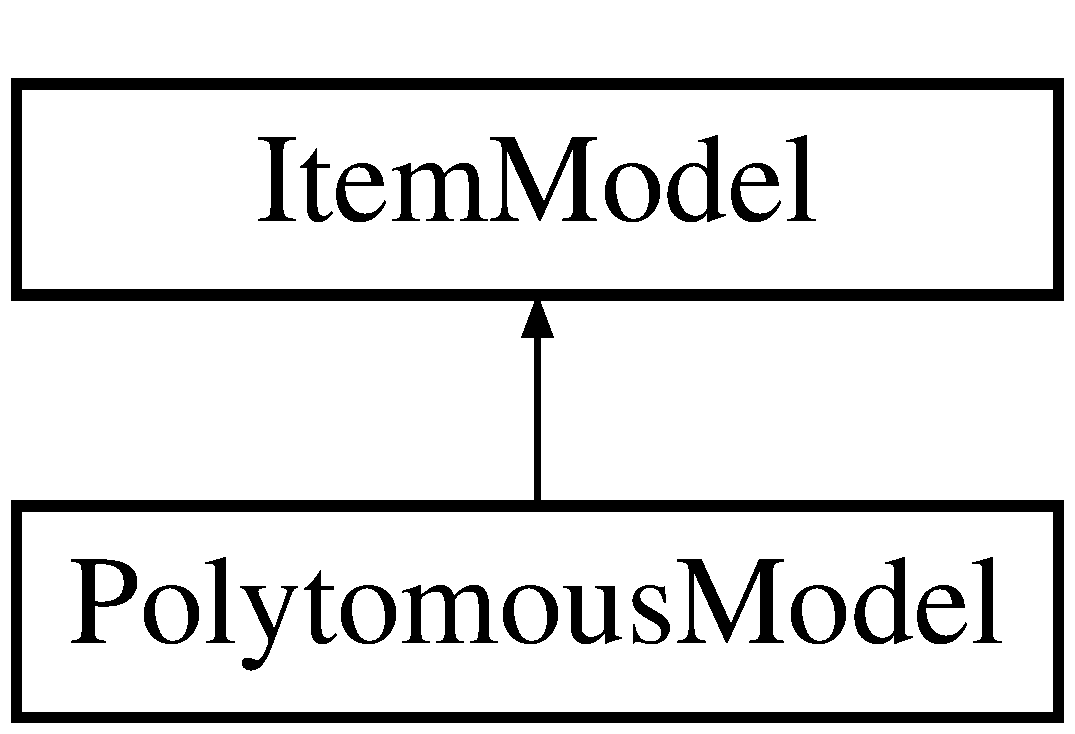
\includegraphics[height=2.000000cm]{classPolytomousModel}
\end{center}
\end{figure}
\subsection*{Public Member Functions}
\begin{DoxyCompactItemize}
\item 
\hyperlink{classPolytomousModel_a7eb616216ec5dd988ca59fef6ce79fe6}{Polytomous\+Model} ()
\item 
int \hyperlink{classPolytomousModel_a1a65e5771d53f6921c48fdc41ea62961}{count\+Categories} ()
\item 
int \hyperlink{classPolytomousModel_a8828b2108445ef361a4af0a3aaf07e86}{count\+Items} ()
\item 
\hyperlink{classDataSet}{Data\+Set} $\ast$ \hyperlink{classPolytomousModel_a0e1aa66768478466b3e49a9f54ace8ba}{get\+Dataset} ()
\item 
void \hyperlink{classPolytomousModel_a71b943b552ae6842f94370698fc9ba0b}{set\+Dataset} (\hyperlink{classDataSet}{Data\+Set} $\ast$dataset)
\item 
virtual \hyperlink{classPolytomousModel_a4759a7fca25241fedb8499191ae775ca}{$\sim$\+Polytomous\+Model} ()
\end{DoxyCompactItemize}
\subsection*{Additional Inherited Members}


\subsection{Detailed Description}


Definition at line 13 of file Polytomous\+Model.\+h.



\subsection{Constructor \& Destructor Documentation}
\hypertarget{classPolytomousModel_a7eb616216ec5dd988ca59fef6ce79fe6}{}\index{Polytomous\+Model@{Polytomous\+Model}!Polytomous\+Model@{Polytomous\+Model}}
\index{Polytomous\+Model@{Polytomous\+Model}!Polytomous\+Model@{Polytomous\+Model}}
\subsubsection[{Polytomous\+Model}]{\setlength{\rightskip}{0pt plus 5cm}Polytomous\+Model\+::\+Polytomous\+Model (
\begin{DoxyParamCaption}
{}
\end{DoxyParamCaption}
)}\label{classPolytomousModel_a7eb616216ec5dd988ca59fef6ce79fe6}


Definition at line 10 of file Polytomous\+Model.\+cpp.

\hypertarget{classPolytomousModel_a4759a7fca25241fedb8499191ae775ca}{}\index{Polytomous\+Model@{Polytomous\+Model}!````~Polytomous\+Model@{$\sim$\+Polytomous\+Model}}
\index{````~Polytomous\+Model@{$\sim$\+Polytomous\+Model}!Polytomous\+Model@{Polytomous\+Model}}
\subsubsection[{$\sim$\+Polytomous\+Model}]{\setlength{\rightskip}{0pt plus 5cm}Polytomous\+Model\+::$\sim$\+Polytomous\+Model (
\begin{DoxyParamCaption}
{}
\end{DoxyParamCaption}
)\hspace{0.3cm}{\ttfamily [virtual]}}\label{classPolytomousModel_a4759a7fca25241fedb8499191ae775ca}


Definition at line 31 of file Polytomous\+Model.\+cpp.



\subsection{Member Function Documentation}
\hypertarget{classPolytomousModel_a1a65e5771d53f6921c48fdc41ea62961}{}\index{Polytomous\+Model@{Polytomous\+Model}!count\+Categories@{count\+Categories}}
\index{count\+Categories@{count\+Categories}!Polytomous\+Model@{Polytomous\+Model}}
\subsubsection[{count\+Categories}]{\setlength{\rightskip}{0pt plus 5cm}int Polytomous\+Model\+::count\+Categories (
\begin{DoxyParamCaption}
{}
\end{DoxyParamCaption}
)\hspace{0.3cm}{\ttfamily [virtual]}}\label{classPolytomousModel_a1a65e5771d53f6921c48fdc41ea62961}


Implements \hyperlink{classItemModel_af0aabe9f48c6d111fbcb903cb330fae7}{Item\+Model}.



Definition at line 15 of file Polytomous\+Model.\+cpp.

\hypertarget{classPolytomousModel_a8828b2108445ef361a4af0a3aaf07e86}{}\index{Polytomous\+Model@{Polytomous\+Model}!count\+Items@{count\+Items}}
\index{count\+Items@{count\+Items}!Polytomous\+Model@{Polytomous\+Model}}
\subsubsection[{count\+Items}]{\setlength{\rightskip}{0pt plus 5cm}int Polytomous\+Model\+::count\+Items (
\begin{DoxyParamCaption}
{}
\end{DoxyParamCaption}
)\hspace{0.3cm}{\ttfamily [virtual]}}\label{classPolytomousModel_a8828b2108445ef361a4af0a3aaf07e86}


Implements \hyperlink{classItemModel_a7a93c60e346f4d80f265a4c9e083181d}{Item\+Model}.



Definition at line 27 of file Polytomous\+Model.\+cpp.

\hypertarget{classPolytomousModel_a0e1aa66768478466b3e49a9f54ace8ba}{}\index{Polytomous\+Model@{Polytomous\+Model}!get\+Dataset@{get\+Dataset}}
\index{get\+Dataset@{get\+Dataset}!Polytomous\+Model@{Polytomous\+Model}}
\subsubsection[{get\+Dataset}]{\setlength{\rightskip}{0pt plus 5cm}{\bf Data\+Set} $\ast$ Polytomous\+Model\+::get\+Dataset (
\begin{DoxyParamCaption}
{}
\end{DoxyParamCaption}
)\hspace{0.3cm}{\ttfamily [virtual]}}\label{classPolytomousModel_a0e1aa66768478466b3e49a9f54ace8ba}


Implements \hyperlink{classItemModel_a8521ea3f8f511e88d5257ff7591cd928}{Item\+Model}.



Definition at line 19 of file Polytomous\+Model.\+cpp.



References Item\+Model\+::data\+Set.

\hypertarget{classPolytomousModel_a71b943b552ae6842f94370698fc9ba0b}{}\index{Polytomous\+Model@{Polytomous\+Model}!set\+Dataset@{set\+Dataset}}
\index{set\+Dataset@{set\+Dataset}!Polytomous\+Model@{Polytomous\+Model}}
\subsubsection[{set\+Dataset}]{\setlength{\rightskip}{0pt plus 5cm}void Polytomous\+Model\+::set\+Dataset (
\begin{DoxyParamCaption}
\item[{{\bf Data\+Set} $\ast$}]{dataset}
\end{DoxyParamCaption}
)\hspace{0.3cm}{\ttfamily [virtual]}}\label{classPolytomousModel_a71b943b552ae6842f94370698fc9ba0b}


Implements \hyperlink{classItemModel_accd6c6b6827c45970d04c22baaca6b0c}{Item\+Model}.



Definition at line 23 of file Polytomous\+Model.\+cpp.



References Item\+Model\+::data\+Set.



The documentation for this class was generated from the following files\+:\begin{DoxyCompactItemize}
\item 
src/model/item/\hyperlink{PolytomousModel_8h}{Polytomous\+Model.\+h}\item 
src/model/item/\hyperlink{PolytomousModel_8cpp}{Polytomous\+Model.\+cpp}\end{DoxyCompactItemize}

\hypertarget{classRaschModel}{}\section{Rasch\+Model Class Reference}
\label{classRaschModel}\index{Rasch\+Model@{Rasch\+Model}}


{\ttfamily \#include $<$Rasch\+Model.\+h$>$}

Inheritance diagram for Rasch\+Model\+:\begin{figure}[H]
\begin{center}
\leavevmode
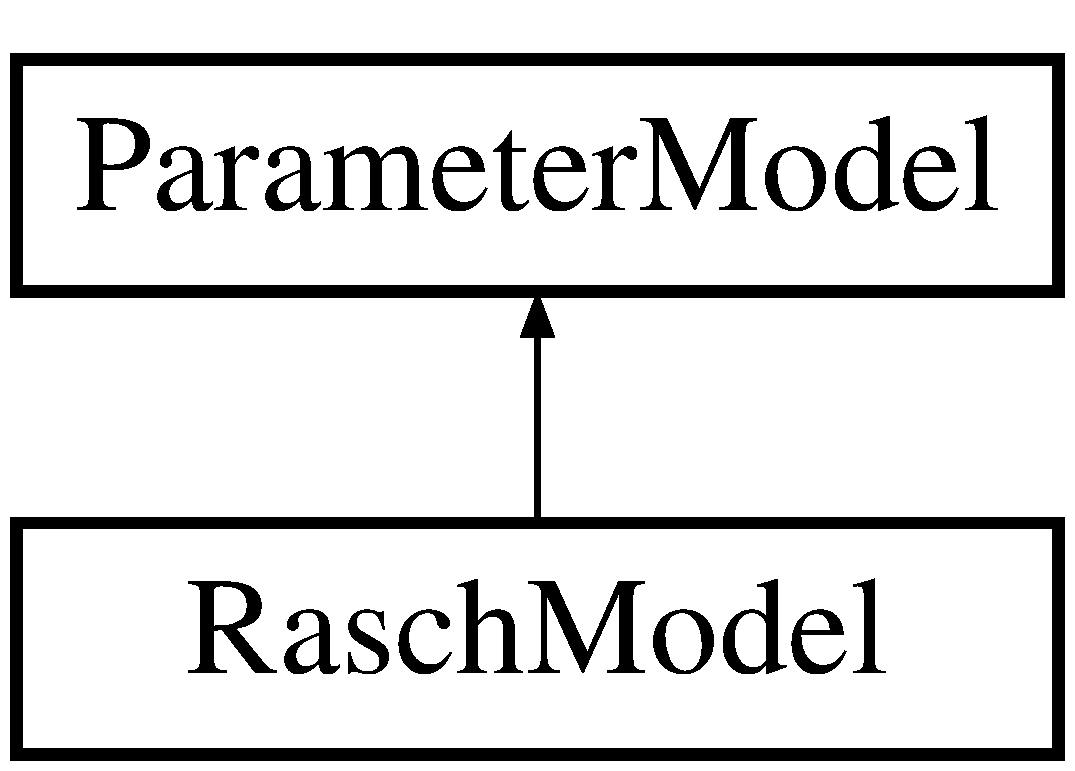
\includegraphics[height=2.000000cm]{classRaschModel}
\end{center}
\end{figure}
\subsection*{Public Member Functions}
\begin{DoxyCompactItemize}
\item 
\hyperlink{classRaschModel_ab4efbe6df1d5dad527d4ff7ac7637033}{Rasch\+Model} ()
\item 
void \hyperlink{classRaschModel_a73b865f129db10fb7ba74495c3fce60b}{build\+Parameter\+Set} (\hyperlink{classItemModel}{Item\+Model} $\ast$, \hyperlink{classDimensionModel}{Dimension\+Model} $\ast$)
\item 
void \hyperlink{classRaschModel_a3d082fd28aa10277623dd665d2127d64}{success\+Probability} (\hyperlink{classDimensionModel}{Dimension\+Model} $\ast$)
\item 
map$<$ \hyperlink{ParameterModel_8h_a04ed5b8f1f3adf7af1d5092fae847e90}{Parameter}, \hyperlink{singletonMatrix}{Matrix}$<$ double $>$ $\ast$ $>$ \hyperlink{classRaschModel_aee54609e4db0cb065dc1761e787e8ba9}{get\+Parameter\+Set} ()
\item 
void \hyperlink{classRaschModel_a3c4614d2536c807cea40df2301c063ca}{set\+Parameter\+Set} (map$<$ \hyperlink{ParameterModel_8h_a04ed5b8f1f3adf7af1d5092fae847e90}{Parameter}, \hyperlink{singletonMatrix}{Matrix}$<$ double $>$ $\ast$ $>$)
\item 
double \hyperlink{classRaschModel_ae9a8edbdf6d1e5b801fb291b7035fc79}{get\+Probability} (int, int)
\item 
virtual \hyperlink{classRaschModel_aad14886beb9250bf60ecb44009fee0b2}{$\sim$\+Rasch\+Model} ()
\end{DoxyCompactItemize}
\subsection*{Additional Inherited Members}


\subsection{Detailed Description}


Definition at line 13 of file Rasch\+Model.\+h.



\subsection{Constructor \& Destructor Documentation}
\hypertarget{classRaschModel_ab4efbe6df1d5dad527d4ff7ac7637033}{}\index{Rasch\+Model@{Rasch\+Model}!Rasch\+Model@{Rasch\+Model}}
\index{Rasch\+Model@{Rasch\+Model}!Rasch\+Model@{Rasch\+Model}}
\subsubsection[{Rasch\+Model}]{\setlength{\rightskip}{0pt plus 5cm}Rasch\+Model\+::\+Rasch\+Model (
\begin{DoxyParamCaption}
{}
\end{DoxyParamCaption}
)}\label{classRaschModel_ab4efbe6df1d5dad527d4ff7ac7637033}


Definition at line 10 of file Rasch\+Model.\+cpp.

\hypertarget{classRaschModel_aad14886beb9250bf60ecb44009fee0b2}{}\index{Rasch\+Model@{Rasch\+Model}!````~Rasch\+Model@{$\sim$\+Rasch\+Model}}
\index{````~Rasch\+Model@{$\sim$\+Rasch\+Model}!Rasch\+Model@{Rasch\+Model}}
\subsubsection[{$\sim$\+Rasch\+Model}]{\setlength{\rightskip}{0pt plus 5cm}Rasch\+Model\+::$\sim$\+Rasch\+Model (
\begin{DoxyParamCaption}
{}
\end{DoxyParamCaption}
)\hspace{0.3cm}{\ttfamily [virtual]}}\label{classRaschModel_aad14886beb9250bf60ecb44009fee0b2}


Definition at line 33 of file Rasch\+Model.\+cpp.



\subsection{Member Function Documentation}
\hypertarget{classRaschModel_a73b865f129db10fb7ba74495c3fce60b}{}\index{Rasch\+Model@{Rasch\+Model}!build\+Parameter\+Set@{build\+Parameter\+Set}}
\index{build\+Parameter\+Set@{build\+Parameter\+Set}!Rasch\+Model@{Rasch\+Model}}
\subsubsection[{build\+Parameter\+Set}]{\setlength{\rightskip}{0pt plus 5cm}void Rasch\+Model\+::build\+Parameter\+Set (
\begin{DoxyParamCaption}
\item[{{\bf Item\+Model} $\ast$}]{, }
\item[{{\bf Dimension\+Model} $\ast$}]{}
\end{DoxyParamCaption}
)\hspace{0.3cm}{\ttfamily [virtual]}}\label{classRaschModel_a73b865f129db10fb7ba74495c3fce60b}


Implements \hyperlink{classParameterModel_a2f02140d0b27796ccdaf9cadbccb2e2f}{Parameter\+Model}.



Definition at line 15 of file Rasch\+Model.\+cpp.

\hypertarget{classRaschModel_aee54609e4db0cb065dc1761e787e8ba9}{}\index{Rasch\+Model@{Rasch\+Model}!get\+Parameter\+Set@{get\+Parameter\+Set}}
\index{get\+Parameter\+Set@{get\+Parameter\+Set}!Rasch\+Model@{Rasch\+Model}}
\subsubsection[{get\+Parameter\+Set}]{\setlength{\rightskip}{0pt plus 5cm}map$<$ {\bf Parameter}, {\bf Matrix}$<$ double $>$ $\ast$ $>$ Rasch\+Model\+::get\+Parameter\+Set (
\begin{DoxyParamCaption}
{}
\end{DoxyParamCaption}
)\hspace{0.3cm}{\ttfamily [virtual]}}\label{classRaschModel_aee54609e4db0cb065dc1761e787e8ba9}


Implements \hyperlink{classParameterModel_aa4e52819318c9dcc9087a36d1a940c0b}{Parameter\+Model}.



Definition at line 25 of file Rasch\+Model.\+cpp.



References Parameter\+Model\+::parameter\+Set.

\hypertarget{classRaschModel_ae9a8edbdf6d1e5b801fb291b7035fc79}{}\index{Rasch\+Model@{Rasch\+Model}!get\+Probability@{get\+Probability}}
\index{get\+Probability@{get\+Probability}!Rasch\+Model@{Rasch\+Model}}
\subsubsection[{get\+Probability}]{\setlength{\rightskip}{0pt plus 5cm}double Rasch\+Model\+::get\+Probability (
\begin{DoxyParamCaption}
\item[{int}]{node, }
\item[{int}]{item}
\end{DoxyParamCaption}
)\hspace{0.3cm}{\ttfamily [virtual]}}\label{classRaschModel_ae9a8edbdf6d1e5b801fb291b7035fc79}


Implements \hyperlink{classParameterModel_ac706c102c88bb20f5d47e61eb8d5dc7e}{Parameter\+Model}.



Definition at line 29 of file Rasch\+Model.\+cpp.

\hypertarget{classRaschModel_a3c4614d2536c807cea40df2301c063ca}{}\index{Rasch\+Model@{Rasch\+Model}!set\+Parameter\+Set@{set\+Parameter\+Set}}
\index{set\+Parameter\+Set@{set\+Parameter\+Set}!Rasch\+Model@{Rasch\+Model}}
\subsubsection[{set\+Parameter\+Set}]{\setlength{\rightskip}{0pt plus 5cm}void Rasch\+Model\+::set\+Parameter\+Set (
\begin{DoxyParamCaption}
\item[{map$<$ {\bf Parameter}, {\bf Matrix}$<$ double $>$ $\ast$ $>$}]{pair}
\end{DoxyParamCaption}
)\hspace{0.3cm}{\ttfamily [virtual]}}\label{classRaschModel_a3c4614d2536c807cea40df2301c063ca}


Implements \hyperlink{classParameterModel_aa13375bcd79d7c1afbde0a8f179f38cb}{Parameter\+Model}.



Definition at line 21 of file Rasch\+Model.\+cpp.



References Parameter\+Model\+::parameter\+Set.

\hypertarget{classRaschModel_a3d082fd28aa10277623dd665d2127d64}{}\index{Rasch\+Model@{Rasch\+Model}!success\+Probability@{success\+Probability}}
\index{success\+Probability@{success\+Probability}!Rasch\+Model@{Rasch\+Model}}
\subsubsection[{success\+Probability}]{\setlength{\rightskip}{0pt plus 5cm}void Rasch\+Model\+::success\+Probability (
\begin{DoxyParamCaption}
\item[{{\bf Dimension\+Model} $\ast$}]{}
\end{DoxyParamCaption}
)\hspace{0.3cm}{\ttfamily [virtual]}}\label{classRaschModel_a3d082fd28aa10277623dd665d2127d64}


Implements \hyperlink{classParameterModel_a13249755ab9078be82262896beff5c17}{Parameter\+Model}.



Definition at line 18 of file Rasch\+Model.\+cpp.



The documentation for this class was generated from the following files\+:\begin{DoxyCompactItemize}
\item 
src/model/parameter/\hyperlink{RaschModel_8h}{Rasch\+Model.\+h}\item 
src/model/parameter/\hyperlink{RaschModel_8cpp}{Rasch\+Model.\+cpp}\end{DoxyCompactItemize}

\hypertarget{classSICSGeneralModel}{}\section{S\+I\+C\+S\+General\+Model Class Reference}
\label{classSICSGeneralModel}\index{S\+I\+C\+S\+General\+Model@{S\+I\+C\+S\+General\+Model}}


{\ttfamily \#include $<$S\+I\+C\+S\+General\+Model.\+h$>$}

Inheritance diagram for S\+I\+C\+S\+General\+Model\+:\begin{figure}[H]
\begin{center}
\leavevmode
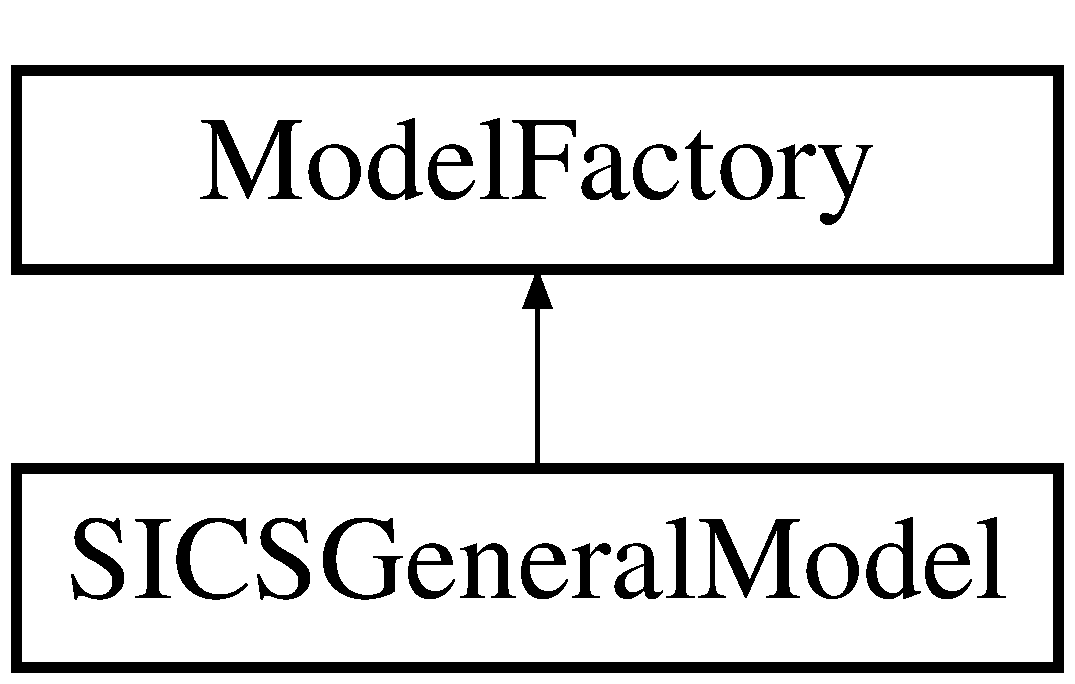
\includegraphics[height=2.000000cm]{classSICSGeneralModel}
\end{center}
\end{figure}
\subsection*{Public Member Functions}
\begin{DoxyCompactItemize}
\item 
\hyperlink{classSICSGeneralModel_a3d19adad0cd3cf346af4ab4486234f55}{S\+I\+C\+S\+General\+Model} ()
\item 
\hyperlink{classParameterModel}{Parameter\+Model} $\ast$ \hyperlink{classSICSGeneralModel_ac494be453a5c9213bfa1a959b1c985f1}{create\+Parameter\+Model} ()
\item 
\hyperlink{classItemModel}{Item\+Model} $\ast$ \hyperlink{classSICSGeneralModel_ae6d6f2faf2b10bc67114be9d742d354e}{create\+Item\+Model} ()
\item 
\hyperlink{classDimensionModel}{Dimension\+Model} $\ast$ \hyperlink{classSICSGeneralModel_a35ec6c2939eba08e663a7c0b99d796a2}{create\+Dimension\+Model} ()
\item 
virtual \hyperlink{classSICSGeneralModel_a3127ef946fd974f8efdea1e205999e0a}{$\sim$\+S\+I\+C\+S\+General\+Model} ()
\end{DoxyCompactItemize}


\subsection{Detailed Description}


Definition at line 16 of file S\+I\+C\+S\+General\+Model.\+h.



\subsection{Constructor \& Destructor Documentation}
\hypertarget{classSICSGeneralModel_a3d19adad0cd3cf346af4ab4486234f55}{}\index{S\+I\+C\+S\+General\+Model@{S\+I\+C\+S\+General\+Model}!S\+I\+C\+S\+General\+Model@{S\+I\+C\+S\+General\+Model}}
\index{S\+I\+C\+S\+General\+Model@{S\+I\+C\+S\+General\+Model}!S\+I\+C\+S\+General\+Model@{S\+I\+C\+S\+General\+Model}}
\subsubsection[{S\+I\+C\+S\+General\+Model}]{\setlength{\rightskip}{0pt plus 5cm}S\+I\+C\+S\+General\+Model\+::\+S\+I\+C\+S\+General\+Model (
\begin{DoxyParamCaption}
{}
\end{DoxyParamCaption}
)}\label{classSICSGeneralModel_a3d19adad0cd3cf346af4ab4486234f55}


Definition at line 10 of file S\+I\+C\+S\+General\+Model.\+cpp.

\hypertarget{classSICSGeneralModel_a3127ef946fd974f8efdea1e205999e0a}{}\index{S\+I\+C\+S\+General\+Model@{S\+I\+C\+S\+General\+Model}!````~S\+I\+C\+S\+General\+Model@{$\sim$\+S\+I\+C\+S\+General\+Model}}
\index{````~S\+I\+C\+S\+General\+Model@{$\sim$\+S\+I\+C\+S\+General\+Model}!S\+I\+C\+S\+General\+Model@{S\+I\+C\+S\+General\+Model}}
\subsubsection[{$\sim$\+S\+I\+C\+S\+General\+Model}]{\setlength{\rightskip}{0pt plus 5cm}S\+I\+C\+S\+General\+Model\+::$\sim$\+S\+I\+C\+S\+General\+Model (
\begin{DoxyParamCaption}
{}
\end{DoxyParamCaption}
)\hspace{0.3cm}{\ttfamily [virtual]}}\label{classSICSGeneralModel_a3127ef946fd974f8efdea1e205999e0a}


Definition at line 30 of file S\+I\+C\+S\+General\+Model.\+cpp.



\subsection{Member Function Documentation}
\hypertarget{classSICSGeneralModel_a35ec6c2939eba08e663a7c0b99d796a2}{}\index{S\+I\+C\+S\+General\+Model@{S\+I\+C\+S\+General\+Model}!create\+Dimension\+Model@{create\+Dimension\+Model}}
\index{create\+Dimension\+Model@{create\+Dimension\+Model}!S\+I\+C\+S\+General\+Model@{S\+I\+C\+S\+General\+Model}}
\subsubsection[{create\+Dimension\+Model}]{\setlength{\rightskip}{0pt plus 5cm}{\bf Dimension\+Model} $\ast$ S\+I\+C\+S\+General\+Model\+::create\+Dimension\+Model (
\begin{DoxyParamCaption}
{}
\end{DoxyParamCaption}
)\hspace{0.3cm}{\ttfamily [virtual]}}\label{classSICSGeneralModel_a35ec6c2939eba08e663a7c0b99d796a2}


Implements \hyperlink{classModelFactory_ae57ccc96f948d4df70cebc587ed0390b}{Model\+Factory}.



Definition at line 25 of file S\+I\+C\+S\+General\+Model.\+cpp.

\hypertarget{classSICSGeneralModel_ae6d6f2faf2b10bc67114be9d742d354e}{}\index{S\+I\+C\+S\+General\+Model@{S\+I\+C\+S\+General\+Model}!create\+Item\+Model@{create\+Item\+Model}}
\index{create\+Item\+Model@{create\+Item\+Model}!S\+I\+C\+S\+General\+Model@{S\+I\+C\+S\+General\+Model}}
\subsubsection[{create\+Item\+Model}]{\setlength{\rightskip}{0pt plus 5cm}{\bf Item\+Model} $\ast$ S\+I\+C\+S\+General\+Model\+::create\+Item\+Model (
\begin{DoxyParamCaption}
{}
\end{DoxyParamCaption}
)\hspace{0.3cm}{\ttfamily [virtual]}}\label{classSICSGeneralModel_ae6d6f2faf2b10bc67114be9d742d354e}


Implements \hyperlink{classModelFactory_ab13ed21aabab9b4ba77173d0117a7cec}{Model\+Factory}.



Definition at line 20 of file S\+I\+C\+S\+General\+Model.\+cpp.

\hypertarget{classSICSGeneralModel_ac494be453a5c9213bfa1a959b1c985f1}{}\index{S\+I\+C\+S\+General\+Model@{S\+I\+C\+S\+General\+Model}!create\+Parameter\+Model@{create\+Parameter\+Model}}
\index{create\+Parameter\+Model@{create\+Parameter\+Model}!S\+I\+C\+S\+General\+Model@{S\+I\+C\+S\+General\+Model}}
\subsubsection[{create\+Parameter\+Model}]{\setlength{\rightskip}{0pt plus 5cm}{\bf Parameter\+Model} $\ast$ S\+I\+C\+S\+General\+Model\+::create\+Parameter\+Model (
\begin{DoxyParamCaption}
{}
\end{DoxyParamCaption}
)\hspace{0.3cm}{\ttfamily [virtual]}}\label{classSICSGeneralModel_ac494be453a5c9213bfa1a959b1c985f1}


Implements \hyperlink{classModelFactory_adfa2a321dba41b9ba05e7805b9bfac2b}{Model\+Factory}.



Definition at line 15 of file S\+I\+C\+S\+General\+Model.\+cpp.



The documentation for this class was generated from the following files\+:\begin{DoxyCompactItemize}
\item 
src/model/\hyperlink{SICSGeneralModel_8h}{S\+I\+C\+S\+General\+Model.\+h}\item 
src/model/\hyperlink{SICSGeneralModel_8cpp}{S\+I\+C\+S\+General\+Model.\+cpp}\end{DoxyCompactItemize}

\hypertarget{classSymmetricMatrix}{}\section{Symmetric\+Matrix Class Reference}
\label{classSymmetricMatrix}\index{Symmetric\+Matrix@{Symmetric\+Matrix}}


{\ttfamily \#include $<$Symmetric\+Matrix.\+h$>$}

\subsection*{Public Member Functions}
\begin{DoxyCompactItemize}
\item 
\hyperlink{classSymmetricMatrix_a74050d9aa95d68b583c115146dda9387}{Symmetric\+Matrix} ()
\item 
virtual \hyperlink{classSymmetricMatrix_a27e50f8c308d10f1f69ceb6803e78021}{$\sim$\+Symmetric\+Matrix} ()
\end{DoxyCompactItemize}


\subsection{Detailed Description}


Definition at line 11 of file Symmetric\+Matrix.\+h.



\subsection{Constructor \& Destructor Documentation}
\hypertarget{classSymmetricMatrix_a74050d9aa95d68b583c115146dda9387}{}\index{Symmetric\+Matrix@{Symmetric\+Matrix}!Symmetric\+Matrix@{Symmetric\+Matrix}}
\index{Symmetric\+Matrix@{Symmetric\+Matrix}!Symmetric\+Matrix@{Symmetric\+Matrix}}
\subsubsection[{Symmetric\+Matrix}]{\setlength{\rightskip}{0pt plus 5cm}Symmetric\+Matrix\+::\+Symmetric\+Matrix (
\begin{DoxyParamCaption}
{}
\end{DoxyParamCaption}
)}\label{classSymmetricMatrix_a74050d9aa95d68b583c115146dda9387}


Definition at line 10 of file Symmetric\+Matrix.\+cpp.

\hypertarget{classSymmetricMatrix_a27e50f8c308d10f1f69ceb6803e78021}{}\index{Symmetric\+Matrix@{Symmetric\+Matrix}!````~Symmetric\+Matrix@{$\sim$\+Symmetric\+Matrix}}
\index{````~Symmetric\+Matrix@{$\sim$\+Symmetric\+Matrix}!Symmetric\+Matrix@{Symmetric\+Matrix}}
\subsubsection[{$\sim$\+Symmetric\+Matrix}]{\setlength{\rightskip}{0pt plus 5cm}Symmetric\+Matrix\+::$\sim$\+Symmetric\+Matrix (
\begin{DoxyParamCaption}
{}
\end{DoxyParamCaption}
)\hspace{0.3cm}{\ttfamily [virtual]}}\label{classSymmetricMatrix_a27e50f8c308d10f1f69ceb6803e78021}


Definition at line 15 of file Symmetric\+Matrix.\+cpp.



The documentation for this class was generated from the following files\+:\begin{DoxyCompactItemize}
\item 
src/type/matrix/\hyperlink{SymmetricMatrix_8h}{Symmetric\+Matrix.\+h}\item 
src/type/matrix/\hyperlink{SymmetricMatrix_8cpp}{Symmetric\+Matrix.\+cpp}\end{DoxyCompactItemize}

\hypertarget{classThreePLModel}{}\section{Three\+P\+L\+Model Class Reference}
\label{classThreePLModel}\index{Three\+P\+L\+Model@{Three\+P\+L\+Model}}


\hyperlink{classModel}{Model} for the 3pl model, uses parameters a d c.  




{\ttfamily \#include $<$Three\+P\+L\+Model.\+h$>$}

Inheritance diagram for Three\+P\+L\+Model\+:\begin{figure}[H]
\begin{center}
\leavevmode
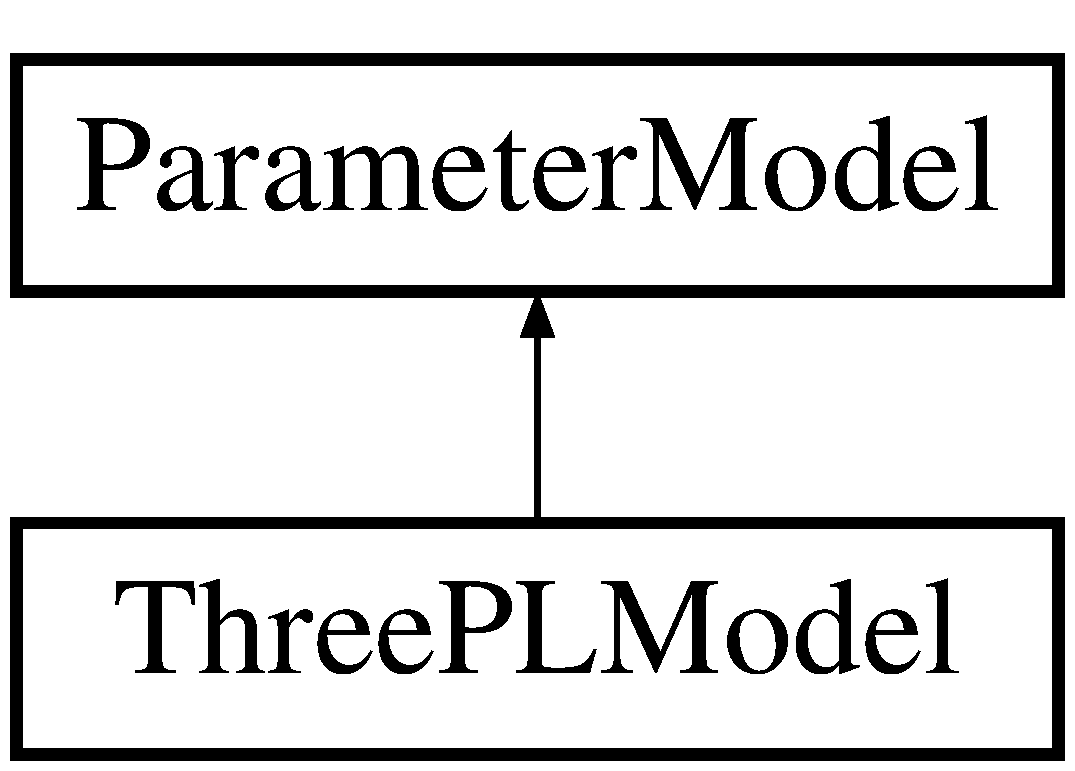
\includegraphics[height=2.000000cm]{classThreePLModel}
\end{center}
\end{figure}
\subsection*{Public Member Functions}
\begin{DoxyCompactItemize}
\item 
\hyperlink{classThreePLModel_a97470c701290327dc55b87a10874156c}{Three\+P\+L\+Model} ()
\item 
void \hyperlink{classThreePLModel_a7242d2bf961e6bf167cc7ca89cf36a67}{build\+Parameter\+Set} (\hyperlink{classItemModel}{Item\+Model} $\ast$, \hyperlink{classDimensionModel}{Dimension\+Model} $\ast$)
\item 
void \hyperlink{classThreePLModel_a983cdd653542d76b150c502ac88a3a0d}{success\+Probability} (\hyperlink{classDimensionModel}{Dimension\+Model} $\ast$)
\item 
map$<$ \hyperlink{ParameterModel_8h_a04ed5b8f1f3adf7af1d5092fae847e90}{Parameter}, \hyperlink{singletonMatrix}{Matrix}$<$ double $>$ $\ast$ $>$ \hyperlink{classThreePLModel_ae87fb19a09c536da3fb9cbbfc443bc8e}{get\+Parameter\+Set} ()
\item 
void \hyperlink{classThreePLModel_aa049135b26ea1a9f81f23dfac6195696}{set\+Parameter\+Set} (map$<$ \hyperlink{ParameterModel_8h_a04ed5b8f1f3adf7af1d5092fae847e90}{Parameter}, \hyperlink{singletonMatrix}{Matrix}$<$ double $>$ $\ast$ $>$)
\item 
double \hyperlink{classThreePLModel_a36cdc7dc2e7b009a54c773de3645707b}{get\+Probability} (int, int)
\item 
virtual \hyperlink{classThreePLModel_a146e9c48084c708708060cf433346f1b}{$\sim$\+Three\+P\+L\+Model} ()
\end{DoxyCompactItemize}
\subsection*{Static Public Member Functions}
\begin{DoxyCompactItemize}
\item 
static double \hyperlink{classThreePLModel_a4ac3badc7d7a17b57be43d24bfb924e3}{success\+Probability} (double, double, double, double)
\item 
static double \hyperlink{classThreePLModel_a89d3c2a8f9d077e48db38f78aa8d3526}{success\+Probability\+\_\+c\+Prime} (double, double, double, double)
\item 
static double \hyperlink{classThreePLModel_ae31380f753f4bc118788f9dbc93fe4af}{log\+Likelihood} (double $\ast$, double $\ast$, int, int)
\item 
static void \hyperlink{classThreePLModel_a6b86ab6fe2c11047723864ab95bd29da}{gradient} (double $\ast$, double $\ast$, int, int, double $\ast$)
\item 
static void \hyperlink{classThreePLModel_ae24fa3d2b9bf02b79a010ea760f1bff4}{Ngradient} (double $\ast$args, double $\ast$pars, int nargs, int npars, double $\ast$\hyperlink{classThreePLModel_a6b86ab6fe2c11047723864ab95bd29da}{gradient})
\item 
static void \hyperlink{classThreePLModel_a034561892349c03922d857a67d15f79d}{Hessian} (double $\ast$args, double $\ast$pars, int nargs, int npars, double $\ast$Hessian)
\item 
static void \hyperlink{classThreePLModel_acc5f243d6863cf431df88b4b1648e52d}{N\+Hessian} (double $\ast$args, double $\ast$pars, int nargs, int npars, double $\ast$\hyperlink{classThreePLModel_a034561892349c03922d857a67d15f79d}{Hessian})
\item 
static void \hyperlink{classThreePLModel_a4eb5d27957e207af988cfc87b1adbb27}{item\+Hessian} (double $\ast$args, double $\ast$pars, int nargs, int npars, double $\ast$\hyperlink{classThreePLModel_a034561892349c03922d857a67d15f79d}{Hessian})
\item 
static void \hyperlink{classThreePLModel_a1e103a8afde4c931b15d451f131ebc6e}{itemgradient} (double $\ast$, double $\ast$, int, int, double $\ast$)
\begin{DoxyCompactList}\small\item\em In the item gradient and hessians these procedures take an already calculated hessian and gradient and just access the item that is needed in the optimization step args will then be the ith args for the item pars is going to be the full array of gradients and npars is going to be used to take the ith element the gradient will then be copied to g. \end{DoxyCompactList}\end{DoxyCompactItemize}
\subsection*{Additional Inherited Members}


\subsection{Detailed Description}
\hyperlink{classModel}{Model} for the 3pl model, uses parameters a d c. 

unidimensional 

Definition at line 25 of file Three\+P\+L\+Model.\+h.



\subsection{Constructor \& Destructor Documentation}
\hypertarget{classThreePLModel_a97470c701290327dc55b87a10874156c}{}\index{Three\+P\+L\+Model@{Three\+P\+L\+Model}!Three\+P\+L\+Model@{Three\+P\+L\+Model}}
\index{Three\+P\+L\+Model@{Three\+P\+L\+Model}!Three\+P\+L\+Model@{Three\+P\+L\+Model}}
\subsubsection[{Three\+P\+L\+Model}]{\setlength{\rightskip}{0pt plus 5cm}Three\+P\+L\+Model\+::\+Three\+P\+L\+Model (
\begin{DoxyParamCaption}
{}
\end{DoxyParamCaption}
)}\label{classThreePLModel_a97470c701290327dc55b87a10874156c}


Definition at line 10 of file Three\+P\+L\+Model.\+cpp.



References a, b, c, d, Parameter\+Model\+::parameter\+Set, and Parameter\+Model\+::probability\+Matrix.

\hypertarget{classThreePLModel_a146e9c48084c708708060cf433346f1b}{}\index{Three\+P\+L\+Model@{Three\+P\+L\+Model}!````~Three\+P\+L\+Model@{$\sim$\+Three\+P\+L\+Model}}
\index{````~Three\+P\+L\+Model@{$\sim$\+Three\+P\+L\+Model}!Three\+P\+L\+Model@{Three\+P\+L\+Model}}
\subsubsection[{$\sim$\+Three\+P\+L\+Model}]{\setlength{\rightskip}{0pt plus 5cm}Three\+P\+L\+Model\+::$\sim$\+Three\+P\+L\+Model (
\begin{DoxyParamCaption}
{}
\end{DoxyParamCaption}
)\hspace{0.3cm}{\ttfamily [virtual]}}\label{classThreePLModel_a146e9c48084c708708060cf433346f1b}


Definition at line 617 of file Three\+P\+L\+Model.\+cpp.



References a, b, c, d, and Parameter\+Model\+::parameter\+Set.



\subsection{Member Function Documentation}
\hypertarget{classThreePLModel_a7242d2bf961e6bf167cc7ca89cf36a67}{}\index{Three\+P\+L\+Model@{Three\+P\+L\+Model}!build\+Parameter\+Set@{build\+Parameter\+Set}}
\index{build\+Parameter\+Set@{build\+Parameter\+Set}!Three\+P\+L\+Model@{Three\+P\+L\+Model}}
\subsubsection[{build\+Parameter\+Set}]{\setlength{\rightskip}{0pt plus 5cm}void Three\+P\+L\+Model\+::build\+Parameter\+Set (
\begin{DoxyParamCaption}
\item[{{\bf Item\+Model} $\ast$}]{item\+Model, }
\item[{{\bf Dimension\+Model} $\ast$}]{dimension\+Model}
\end{DoxyParamCaption}
)\hspace{0.3cm}{\ttfamily [virtual]}}\label{classThreePLModel_a7242d2bf961e6bf167cc7ca89cf36a67}


Implements \hyperlink{classParameterModel_a2f02140d0b27796ccdaf9cadbccb2e2f}{Parameter\+Model}.



Definition at line 20 of file Three\+P\+L\+Model.\+cpp.



References a, c, Item\+Model\+::count\+Items(), d, Dimension\+Model\+::get\+Latent\+Trait\+Set(), Latent\+Trait\+Set\+::get\+Theta(), Matrix$<$ T $>$\+::n\+C(), Parameter\+Model\+::parameter\+Set, and Parameter\+Model\+::probability\+Matrix.

\hypertarget{classThreePLModel_ae87fb19a09c536da3fb9cbbfc443bc8e}{}\index{Three\+P\+L\+Model@{Three\+P\+L\+Model}!get\+Parameter\+Set@{get\+Parameter\+Set}}
\index{get\+Parameter\+Set@{get\+Parameter\+Set}!Three\+P\+L\+Model@{Three\+P\+L\+Model}}
\subsubsection[{get\+Parameter\+Set}]{\setlength{\rightskip}{0pt plus 5cm}map$<$ {\bf Parameter}, {\bf Matrix}$<$ double $>$ $\ast$ $>$ Three\+P\+L\+Model\+::get\+Parameter\+Set (
\begin{DoxyParamCaption}
{}
\end{DoxyParamCaption}
)\hspace{0.3cm}{\ttfamily [virtual]}}\label{classThreePLModel_ae87fb19a09c536da3fb9cbbfc443bc8e}


Implements \hyperlink{classParameterModel_aa4e52819318c9dcc9087a36d1a940c0b}{Parameter\+Model}.



Definition at line 81 of file Three\+P\+L\+Model.\+cpp.



References Parameter\+Model\+::parameter\+Set.

\hypertarget{classThreePLModel_a36cdc7dc2e7b009a54c773de3645707b}{}\index{Three\+P\+L\+Model@{Three\+P\+L\+Model}!get\+Probability@{get\+Probability}}
\index{get\+Probability@{get\+Probability}!Three\+P\+L\+Model@{Three\+P\+L\+Model}}
\subsubsection[{get\+Probability}]{\setlength{\rightskip}{0pt plus 5cm}double Three\+P\+L\+Model\+::get\+Probability (
\begin{DoxyParamCaption}
\item[{int}]{node, }
\item[{int}]{item}
\end{DoxyParamCaption}
)\hspace{0.3cm}{\ttfamily [virtual]}}\label{classThreePLModel_a36cdc7dc2e7b009a54c773de3645707b}


Implements \hyperlink{classParameterModel_ac706c102c88bb20f5d47e61eb8d5dc7e}{Parameter\+Model}.



Definition at line 111 of file Three\+P\+L\+Model.\+cpp.



References Parameter\+Model\+::probability\+Matrix.

\hypertarget{classThreePLModel_a6b86ab6fe2c11047723864ab95bd29da}{}\index{Three\+P\+L\+Model@{Three\+P\+L\+Model}!gradient@{gradient}}
\index{gradient@{gradient}!Three\+P\+L\+Model@{Three\+P\+L\+Model}}
\subsubsection[{gradient}]{\setlength{\rightskip}{0pt plus 5cm}void Three\+P\+L\+Model\+::gradient (
\begin{DoxyParamCaption}
\item[{double $\ast$}]{args, }
\item[{double $\ast$}]{pars, }
\item[{int}]{nargs, }
\item[{int}]{npars, }
\item[{double $\ast$}]{gradient}
\end{DoxyParamCaption}
)\hspace{0.3cm}{\ttfamily [static]}}\label{classThreePLModel_a6b86ab6fe2c11047723864ab95bd29da}


Definition at line 378 of file Three\+P\+L\+Model.\+cpp.



References a, b, c, Constant\+::\+N\+O\+R\+M\+\_\+\+C\+O\+N\+S\+T, and success\+Probability().



Referenced by N\+Hessian(), and E\+M\+Estimation\+::step\+M().

\hypertarget{classThreePLModel_a034561892349c03922d857a67d15f79d}{}\index{Three\+P\+L\+Model@{Three\+P\+L\+Model}!Hessian@{Hessian}}
\index{Hessian@{Hessian}!Three\+P\+L\+Model@{Three\+P\+L\+Model}}
\subsubsection[{Hessian}]{\setlength{\rightskip}{0pt plus 5cm}void Three\+P\+L\+Model\+::\+Hessian (
\begin{DoxyParamCaption}
\item[{double $\ast$}]{args, }
\item[{double $\ast$}]{pars, }
\item[{int}]{nargs, }
\item[{int}]{npars, }
\item[{double $\ast$}]{Hessian}
\end{DoxyParamCaption}
)\hspace{0.3cm}{\ttfamily [static]}}\label{classThreePLModel_a034561892349c03922d857a67d15f79d}


Definition at line 139 of file Three\+P\+L\+Model.\+cpp.



References a, b, c, Constant\+::\+N\+O\+R\+M\+\_\+\+C\+O\+N\+S\+T, and success\+Probability().



Referenced by E\+M\+Estimation\+::step\+M().

\hypertarget{classThreePLModel_a1e103a8afde4c931b15d451f131ebc6e}{}\index{Three\+P\+L\+Model@{Three\+P\+L\+Model}!itemgradient@{itemgradient}}
\index{itemgradient@{itemgradient}!Three\+P\+L\+Model@{Three\+P\+L\+Model}}
\subsubsection[{itemgradient}]{\setlength{\rightskip}{0pt plus 5cm}void Three\+P\+L\+Model\+::itemgradient (
\begin{DoxyParamCaption}
\item[{double $\ast$}]{args, }
\item[{double $\ast$}]{grad, }
\item[{int}]{nargs, }
\item[{int}]{i, }
\item[{double $\ast$}]{tgrad}
\end{DoxyParamCaption}
)\hspace{0.3cm}{\ttfamily [static]}}\label{classThreePLModel_a1e103a8afde4c931b15d451f131ebc6e}


In the item gradient and hessians these procedures take an already calculated hessian and gradient and just access the item that is needed in the optimization step args will then be the ith args for the item pars is going to be the full array of gradients and npars is going to be used to take the ith element the gradient will then be copied to g. 



Definition at line 129 of file Three\+P\+L\+Model.\+cpp.



Referenced by E\+M\+Estimation\+::step\+M().

\hypertarget{classThreePLModel_a4eb5d27957e207af988cfc87b1adbb27}{}\index{Three\+P\+L\+Model@{Three\+P\+L\+Model}!item\+Hessian@{item\+Hessian}}
\index{item\+Hessian@{item\+Hessian}!Three\+P\+L\+Model@{Three\+P\+L\+Model}}
\subsubsection[{item\+Hessian}]{\setlength{\rightskip}{0pt plus 5cm}void Three\+P\+L\+Model\+::item\+Hessian (
\begin{DoxyParamCaption}
\item[{double $\ast$}]{args, }
\item[{double $\ast$}]{pars, }
\item[{int}]{nargs, }
\item[{int}]{npars, }
\item[{double $\ast$}]{Hessian}
\end{DoxyParamCaption}
)\hspace{0.3cm}{\ttfamily [static]}}\label{classThreePLModel_a4eb5d27957e207af988cfc87b1adbb27}


Definition at line 115 of file Three\+P\+L\+Model.\+cpp.



Referenced by E\+M\+Estimation\+::step\+M().

\hypertarget{classThreePLModel_ae31380f753f4bc118788f9dbc93fe4af}{}\index{Three\+P\+L\+Model@{Three\+P\+L\+Model}!log\+Likelihood@{log\+Likelihood}}
\index{log\+Likelihood@{log\+Likelihood}!Three\+P\+L\+Model@{Three\+P\+L\+Model}}
\subsubsection[{log\+Likelihood}]{\setlength{\rightskip}{0pt plus 5cm}double Three\+P\+L\+Model\+::log\+Likelihood (
\begin{DoxyParamCaption}
\item[{double $\ast$}]{args, }
\item[{double $\ast$}]{pars, }
\item[{int}]{nargs, }
\item[{int}]{npars}
\end{DoxyParamCaption}
)\hspace{0.3cm}{\ttfamily [static]}}\label{classThreePLModel_ae31380f753f4bc118788f9dbc93fe4af}


Definition at line 510 of file Three\+P\+L\+Model.\+cpp.



References a, b, c, and success\+Probability().



Referenced by Ngradient(), and E\+M\+Estimation\+::step\+M().

\hypertarget{classThreePLModel_ae24fa3d2b9bf02b79a010ea760f1bff4}{}\index{Three\+P\+L\+Model@{Three\+P\+L\+Model}!Ngradient@{Ngradient}}
\index{Ngradient@{Ngradient}!Three\+P\+L\+Model@{Three\+P\+L\+Model}}
\subsubsection[{Ngradient}]{\setlength{\rightskip}{0pt plus 5cm}void Three\+P\+L\+Model\+::\+Ngradient (
\begin{DoxyParamCaption}
\item[{double $\ast$}]{args, }
\item[{double $\ast$}]{pars, }
\item[{int}]{nargs, }
\item[{int}]{npars, }
\item[{double $\ast$}]{gradient}
\end{DoxyParamCaption}
)\hspace{0.3cm}{\ttfamily [static]}}\label{classThreePLModel_ae24fa3d2b9bf02b79a010ea760f1bff4}


Definition at line 328 of file Three\+P\+L\+Model.\+cpp.



References log\+Likelihood().

\hypertarget{classThreePLModel_acc5f243d6863cf431df88b4b1648e52d}{}\index{Three\+P\+L\+Model@{Three\+P\+L\+Model}!N\+Hessian@{N\+Hessian}}
\index{N\+Hessian@{N\+Hessian}!Three\+P\+L\+Model@{Three\+P\+L\+Model}}
\subsubsection[{N\+Hessian}]{\setlength{\rightskip}{0pt plus 5cm}void Three\+P\+L\+Model\+::\+N\+Hessian (
\begin{DoxyParamCaption}
\item[{double $\ast$}]{args, }
\item[{double $\ast$}]{pars, }
\item[{int}]{nargs, }
\item[{int}]{npars, }
\item[{double $\ast$}]{Hessian}
\end{DoxyParamCaption}
)\hspace{0.3cm}{\ttfamily [static]}}\label{classThreePLModel_acc5f243d6863cf431df88b4b1648e52d}


Definition at line 341 of file Three\+P\+L\+Model.\+cpp.



References gradient().

\hypertarget{classThreePLModel_aa049135b26ea1a9f81f23dfac6195696}{}\index{Three\+P\+L\+Model@{Three\+P\+L\+Model}!set\+Parameter\+Set@{set\+Parameter\+Set}}
\index{set\+Parameter\+Set@{set\+Parameter\+Set}!Three\+P\+L\+Model@{Three\+P\+L\+Model}}
\subsubsection[{set\+Parameter\+Set}]{\setlength{\rightskip}{0pt plus 5cm}void Three\+P\+L\+Model\+::set\+Parameter\+Set (
\begin{DoxyParamCaption}
\item[{map$<$ {\bf Parameter}, {\bf Matrix}$<$ double $>$ $\ast$ $>$}]{parameter\+Set}
\end{DoxyParamCaption}
)\hspace{0.3cm}{\ttfamily [virtual]}}\label{classThreePLModel_aa049135b26ea1a9f81f23dfac6195696}


Implements \hyperlink{classParameterModel_aa13375bcd79d7c1afbde0a8f179f38cb}{Parameter\+Model}.



Definition at line 85 of file Three\+P\+L\+Model.\+cpp.



References Parameter\+Model\+::parameter\+Set.

\hypertarget{classThreePLModel_a4ac3badc7d7a17b57be43d24bfb924e3}{}\index{Three\+P\+L\+Model@{Three\+P\+L\+Model}!success\+Probability@{success\+Probability}}
\index{success\+Probability@{success\+Probability}!Three\+P\+L\+Model@{Three\+P\+L\+Model}}
\subsubsection[{success\+Probability}]{\setlength{\rightskip}{0pt plus 5cm}double Three\+P\+L\+Model\+::success\+Probability (
\begin{DoxyParamCaption}
\item[{double}]{theta, }
\item[{double}]{a, }
\item[{double}]{d, }
\item[{double}]{c}
\end{DoxyParamCaption}
)\hspace{0.3cm}{\ttfamily [static]}}\label{classThreePLModel_a4ac3badc7d7a17b57be43d24bfb924e3}


Definition at line 90 of file Three\+P\+L\+Model.\+cpp.



References Constant\+::\+M\+A\+X\+\_\+\+E\+X\+P, and Constant\+::\+N\+O\+R\+M\+\_\+\+C\+O\+N\+S\+T.



Referenced by gradient(), Hessian(), log\+Likelihood(), success\+Probability(), and success\+Probability\+\_\+c\+Prime().

\hypertarget{classThreePLModel_a983cdd653542d76b150c502ac88a3a0d}{}\index{Three\+P\+L\+Model@{Three\+P\+L\+Model}!success\+Probability@{success\+Probability}}
\index{success\+Probability@{success\+Probability}!Three\+P\+L\+Model@{Three\+P\+L\+Model}}
\subsubsection[{success\+Probability}]{\setlength{\rightskip}{0pt plus 5cm}void Three\+P\+L\+Model\+::success\+Probability (
\begin{DoxyParamCaption}
\item[{{\bf Dimension\+Model} $\ast$}]{dimension\+Model}
\end{DoxyParamCaption}
)\hspace{0.3cm}{\ttfamily [virtual]}}\label{classThreePLModel_a983cdd653542d76b150c502ac88a3a0d}


Implements \hyperlink{classParameterModel_a13249755ab9078be82262896beff5c17}{Parameter\+Model}.



Definition at line 52 of file Three\+P\+L\+Model.\+cpp.



References a, c, d, Dimension\+Model\+::get\+Latent\+Trait\+Set(), Latent\+Trait\+Set\+::get\+Theta(), Matrix$<$ T $>$\+::n\+C(), Parameter\+Model\+::parameter\+Set, and success\+Probability().

\hypertarget{classThreePLModel_a89d3c2a8f9d077e48db38f78aa8d3526}{}\index{Three\+P\+L\+Model@{Three\+P\+L\+Model}!success\+Probability\+\_\+c\+Prime@{success\+Probability\+\_\+c\+Prime}}
\index{success\+Probability\+\_\+c\+Prime@{success\+Probability\+\_\+c\+Prime}!Three\+P\+L\+Model@{Three\+P\+L\+Model}}
\subsubsection[{success\+Probability\+\_\+c\+Prime}]{\setlength{\rightskip}{0pt plus 5cm}double Three\+P\+L\+Model\+::success\+Probability\+\_\+c\+Prime (
\begin{DoxyParamCaption}
\item[{double}]{theta, }
\item[{double}]{a, }
\item[{double}]{b, }
\item[{double}]{c}
\end{DoxyParamCaption}
)\hspace{0.3cm}{\ttfamily [static]}}\label{classThreePLModel_a89d3c2a8f9d077e48db38f78aa8d3526}


Definition at line 611 of file Three\+P\+L\+Model.\+cpp.



References success\+Probability().



The documentation for this class was generated from the following files\+:\begin{DoxyCompactItemize}
\item 
src/model/parameter/\hyperlink{ThreePLModel_8h}{Three\+P\+L\+Model.\+h}\item 
src/model/parameter/\hyperlink{ThreePLModel_8cpp}{Three\+P\+L\+Model.\+cpp}\end{DoxyCompactItemize}

\hypertarget{classTrace}{}\section{Trace Class Reference}
\label{classTrace}\index{Trace@{Trace}}


\hyperlink{classTrace}{Trace} class for constructing execution and error logs onto files.  




{\ttfamily \#include $<$Trace.\+h$>$}

\subsection*{Public Member Functions}
\begin{DoxyCompactItemize}
\item 
\hyperlink{classTrace_ae1caa27c33613b7645a212c31d19bc68}{Trace} (const char $\ast$)
\item 
{\footnotesize template$<$typename T $>$ }\\void \hyperlink{classTrace_aa5e57544d11f722c5dda3ad9a4da6029}{operator()} (\hyperlink{singletonMatrix}{Matrix}$<$ T $>$ \&)
\item 
{\footnotesize template$<$typename T $>$ }\\void \hyperlink{classTrace_af4414b9f6dc073e3f1244ac588b70480}{operator()} (T)
\item 
virtual \hyperlink{classTrace_a39492ecec74969a4905ec5fcf026dc09}{$\sim$\+Trace} ()
\item 
const char $\ast$ \hyperlink{classTrace_afd809a7f04af6e63e65c428409606927}{get\+Filename} () const 
\item 
void \hyperlink{classTrace_a4d8dff9586721e94d2bee132b0739a31}{set\+Filename} (const char $\ast$\hyperlink{classTrace_a0d9910fe66882cafb9617563b397a7b4}{filename})
\end{DoxyCompactItemize}
\subsection*{Private Attributes}
\begin{DoxyCompactItemize}
\item 
const char $\ast$ \hyperlink{classTrace_a0d9910fe66882cafb9617563b397a7b4}{filename}
\end{DoxyCompactItemize}


\subsection{Detailed Description}
\hyperlink{classTrace}{Trace} class for constructing execution and error logs onto files. 

Create a trace with a file to trace to that file when logging errors onto a trace the error logs onto the file asociated trace object can take ostreams, so any output class of cpp can output to the trace 

Definition at line 23 of file Trace.\+h.



\subsection{Constructor \& Destructor Documentation}
\hypertarget{classTrace_ae1caa27c33613b7645a212c31d19bc68}{}\index{Trace@{Trace}!Trace@{Trace}}
\index{Trace@{Trace}!Trace@{Trace}}
\subsubsection[{Trace}]{\setlength{\rightskip}{0pt plus 5cm}Trace\+::\+Trace (
\begin{DoxyParamCaption}
\item[{const char $\ast$}]{filename}
\end{DoxyParamCaption}
)}\label{classTrace_ae1caa27c33613b7645a212c31d19bc68}


Definition at line 10 of file Trace.\+cpp.



References filename.

\hypertarget{classTrace_a39492ecec74969a4905ec5fcf026dc09}{}\index{Trace@{Trace}!````~Trace@{$\sim$\+Trace}}
\index{````~Trace@{$\sim$\+Trace}!Trace@{Trace}}
\subsubsection[{$\sim$\+Trace}]{\setlength{\rightskip}{0pt plus 5cm}Trace\+::$\sim$\+Trace (
\begin{DoxyParamCaption}
{}
\end{DoxyParamCaption}
)\hspace{0.3cm}{\ttfamily [virtual]}}\label{classTrace_a39492ecec74969a4905ec5fcf026dc09}


Definition at line 17 of file Trace.\+cpp.



\subsection{Member Function Documentation}
\hypertarget{classTrace_afd809a7f04af6e63e65c428409606927}{}\index{Trace@{Trace}!get\+Filename@{get\+Filename}}
\index{get\+Filename@{get\+Filename}!Trace@{Trace}}
\subsubsection[{get\+Filename}]{\setlength{\rightskip}{0pt plus 5cm}const char $\ast$ Trace\+::get\+Filename (
\begin{DoxyParamCaption}
{}
\end{DoxyParamCaption}
) const}\label{classTrace_afd809a7f04af6e63e65c428409606927}


Definition at line 21 of file Trace.\+cpp.



References filename.

\hypertarget{classTrace_aa5e57544d11f722c5dda3ad9a4da6029}{}\index{Trace@{Trace}!operator()@{operator()}}
\index{operator()@{operator()}!Trace@{Trace}}
\subsubsection[{operator()}]{\setlength{\rightskip}{0pt plus 5cm}template$<$typename T $>$ void Trace\+::operator() (
\begin{DoxyParamCaption}
\item[{{\bf Matrix}$<$ T $>$ \&}]{message}
\end{DoxyParamCaption}
)}\label{classTrace_aa5e57544d11f722c5dda3ad9a4da6029}


Definition at line 41 of file Trace.\+h.

\hypertarget{classTrace_af4414b9f6dc073e3f1244ac588b70480}{}\index{Trace@{Trace}!operator()@{operator()}}
\index{operator()@{operator()}!Trace@{Trace}}
\subsubsection[{operator()}]{\setlength{\rightskip}{0pt plus 5cm}template$<$typename T $>$ void Trace\+::operator() (
\begin{DoxyParamCaption}
\item[{T}]{message}
\end{DoxyParamCaption}
)}\label{classTrace_af4414b9f6dc073e3f1244ac588b70480}


Definition at line 52 of file Trace.\+h.

\hypertarget{classTrace_a4d8dff9586721e94d2bee132b0739a31}{}\index{Trace@{Trace}!set\+Filename@{set\+Filename}}
\index{set\+Filename@{set\+Filename}!Trace@{Trace}}
\subsubsection[{set\+Filename}]{\setlength{\rightskip}{0pt plus 5cm}void Trace\+::set\+Filename (
\begin{DoxyParamCaption}
\item[{const char $\ast$}]{filename}
\end{DoxyParamCaption}
)}\label{classTrace_a4d8dff9586721e94d2bee132b0739a31}


Definition at line 25 of file Trace.\+cpp.



References filename.



\subsection{Member Data Documentation}
\hypertarget{classTrace_a0d9910fe66882cafb9617563b397a7b4}{}\index{Trace@{Trace}!filename@{filename}}
\index{filename@{filename}!Trace@{Trace}}
\subsubsection[{filename}]{\setlength{\rightskip}{0pt plus 5cm}const char$\ast$ Trace\+::filename\hspace{0.3cm}{\ttfamily [private]}}\label{classTrace_a0d9910fe66882cafb9617563b397a7b4}


Definition at line 24 of file Trace.\+h.



Referenced by get\+Filename(), set\+Filename(), and Trace().



The documentation for this class was generated from the following files\+:\begin{DoxyCompactItemize}
\item 
src/trace/\hyperlink{Trace_8h}{Trace.\+h}\item 
src/trace/\hyperlink{Trace_8cpp}{Trace.\+cpp}\end{DoxyCompactItemize}

\hypertarget{classTwoPLModel}{}\section{Two\+P\+L\+Model Class Reference}
\label{classTwoPLModel}\index{Two\+P\+L\+Model@{Two\+P\+L\+Model}}


{\ttfamily \#include $<$Two\+P\+L\+Model.\+h$>$}

Inheritance diagram for Two\+P\+L\+Model\+:\begin{figure}[H]
\begin{center}
\leavevmode
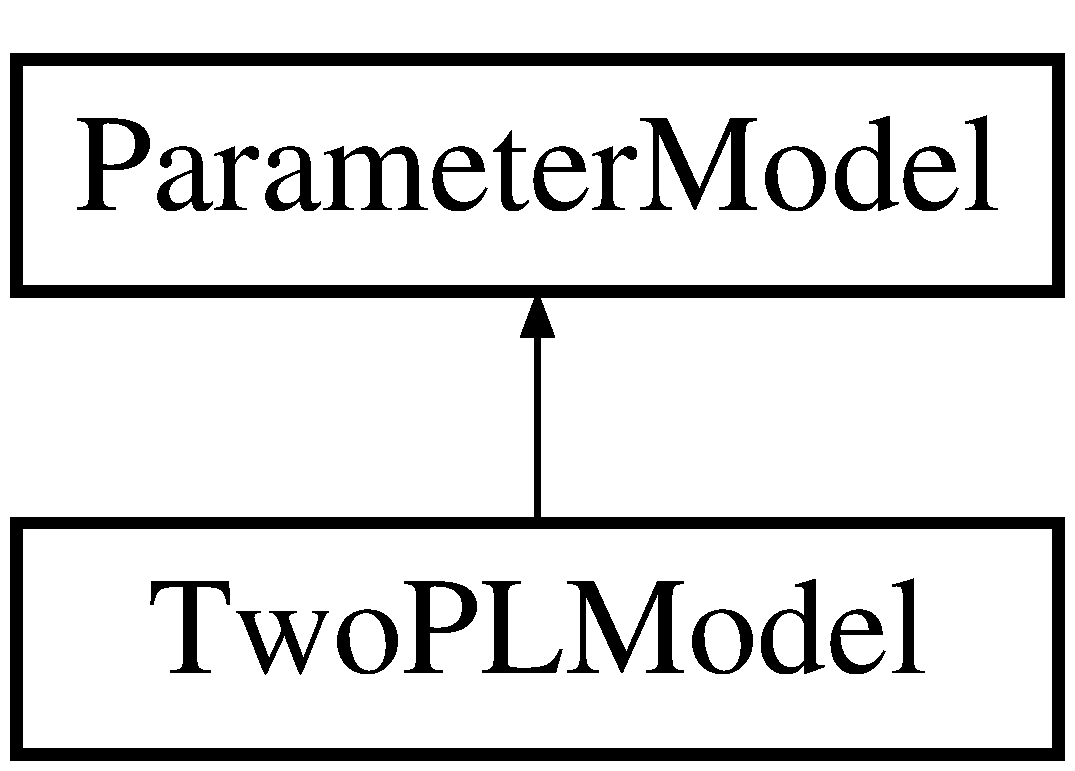
\includegraphics[height=2.000000cm]{classTwoPLModel}
\end{center}
\end{figure}
\subsection*{Public Member Functions}
\begin{DoxyCompactItemize}
\item 
\hyperlink{classTwoPLModel_aba5d80aa87abe92124da11338608b582}{Two\+P\+L\+Model} ()
\item 
void \hyperlink{classTwoPLModel_aabf6941cbcad7f5a73af30725a4bcb31}{build\+Parameter\+Set} (\hyperlink{classItemModel}{Item\+Model} $\ast$, \hyperlink{classDimensionModel}{Dimension\+Model} $\ast$)
\item 
void \hyperlink{classTwoPLModel_a3fb1a6228da24ce1ee7a2bedb6a2f2e7}{success\+Probability} (\hyperlink{classDimensionModel}{Dimension\+Model} $\ast$)
\item 
map$<$ \hyperlink{ParameterModel_8h_a04ed5b8f1f3adf7af1d5092fae847e90}{Parameter}, \hyperlink{singletonMatrix}{Matrix}$<$ double $>$ $\ast$ $>$ \hyperlink{classTwoPLModel_a954cc66bfa5e79838130c09ff2d96edf}{get\+Parameter\+Set} ()
\item 
void \hyperlink{classTwoPLModel_a1a699dcb6b2890e1b2574778c2ec688e}{set\+Parameter\+Set} (map$<$ \hyperlink{ParameterModel_8h_a04ed5b8f1f3adf7af1d5092fae847e90}{Parameter}, \hyperlink{singletonMatrix}{Matrix}$<$ double $>$ $\ast$ $>$)
\item 
double \hyperlink{classTwoPLModel_a89a707b9813ff8c8999267604cc67c62}{get\+Probability} (int, int)
\item 
virtual \hyperlink{classTwoPLModel_aeb4234c3d42b00416c7799027754dde5}{$\sim$\+Two\+P\+L\+Model} ()
\end{DoxyCompactItemize}
\subsection*{Additional Inherited Members}


\subsection{Detailed Description}


Definition at line 13 of file Two\+P\+L\+Model.\+h.



\subsection{Constructor \& Destructor Documentation}
\hypertarget{classTwoPLModel_aba5d80aa87abe92124da11338608b582}{}\index{Two\+P\+L\+Model@{Two\+P\+L\+Model}!Two\+P\+L\+Model@{Two\+P\+L\+Model}}
\index{Two\+P\+L\+Model@{Two\+P\+L\+Model}!Two\+P\+L\+Model@{Two\+P\+L\+Model}}
\subsubsection[{Two\+P\+L\+Model}]{\setlength{\rightskip}{0pt plus 5cm}Two\+P\+L\+Model\+::\+Two\+P\+L\+Model (
\begin{DoxyParamCaption}
{}
\end{DoxyParamCaption}
)}\label{classTwoPLModel_aba5d80aa87abe92124da11338608b582}


Definition at line 10 of file Two\+P\+L\+Model.\+cpp.

\hypertarget{classTwoPLModel_aeb4234c3d42b00416c7799027754dde5}{}\index{Two\+P\+L\+Model@{Two\+P\+L\+Model}!````~Two\+P\+L\+Model@{$\sim$\+Two\+P\+L\+Model}}
\index{````~Two\+P\+L\+Model@{$\sim$\+Two\+P\+L\+Model}!Two\+P\+L\+Model@{Two\+P\+L\+Model}}
\subsubsection[{$\sim$\+Two\+P\+L\+Model}]{\setlength{\rightskip}{0pt plus 5cm}Two\+P\+L\+Model\+::$\sim$\+Two\+P\+L\+Model (
\begin{DoxyParamCaption}
{}
\end{DoxyParamCaption}
)\hspace{0.3cm}{\ttfamily [virtual]}}\label{classTwoPLModel_aeb4234c3d42b00416c7799027754dde5}


Definition at line 33 of file Two\+P\+L\+Model.\+cpp.



\subsection{Member Function Documentation}
\hypertarget{classTwoPLModel_aabf6941cbcad7f5a73af30725a4bcb31}{}\index{Two\+P\+L\+Model@{Two\+P\+L\+Model}!build\+Parameter\+Set@{build\+Parameter\+Set}}
\index{build\+Parameter\+Set@{build\+Parameter\+Set}!Two\+P\+L\+Model@{Two\+P\+L\+Model}}
\subsubsection[{build\+Parameter\+Set}]{\setlength{\rightskip}{0pt plus 5cm}void Two\+P\+L\+Model\+::build\+Parameter\+Set (
\begin{DoxyParamCaption}
\item[{{\bf Item\+Model} $\ast$}]{item\+Model, }
\item[{{\bf Dimension\+Model} $\ast$}]{dimension\+Model}
\end{DoxyParamCaption}
)\hspace{0.3cm}{\ttfamily [virtual]}}\label{classTwoPLModel_aabf6941cbcad7f5a73af30725a4bcb31}


Implements \hyperlink{classParameterModel_a2f02140d0b27796ccdaf9cadbccb2e2f}{Parameter\+Model}.



Definition at line 15 of file Two\+P\+L\+Model.\+cpp.

\hypertarget{classTwoPLModel_a954cc66bfa5e79838130c09ff2d96edf}{}\index{Two\+P\+L\+Model@{Two\+P\+L\+Model}!get\+Parameter\+Set@{get\+Parameter\+Set}}
\index{get\+Parameter\+Set@{get\+Parameter\+Set}!Two\+P\+L\+Model@{Two\+P\+L\+Model}}
\subsubsection[{get\+Parameter\+Set}]{\setlength{\rightskip}{0pt plus 5cm}map$<$ {\bf Parameter}, {\bf Matrix}$<$ double $>$ $\ast$ $>$ Two\+P\+L\+Model\+::get\+Parameter\+Set (
\begin{DoxyParamCaption}
{}
\end{DoxyParamCaption}
)\hspace{0.3cm}{\ttfamily [virtual]}}\label{classTwoPLModel_a954cc66bfa5e79838130c09ff2d96edf}


Implements \hyperlink{classParameterModel_aa4e52819318c9dcc9087a36d1a940c0b}{Parameter\+Model}.



Definition at line 21 of file Two\+P\+L\+Model.\+cpp.



References Parameter\+Model\+::parameter\+Set.

\hypertarget{classTwoPLModel_a89a707b9813ff8c8999267604cc67c62}{}\index{Two\+P\+L\+Model@{Two\+P\+L\+Model}!get\+Probability@{get\+Probability}}
\index{get\+Probability@{get\+Probability}!Two\+P\+L\+Model@{Two\+P\+L\+Model}}
\subsubsection[{get\+Probability}]{\setlength{\rightskip}{0pt plus 5cm}double Two\+P\+L\+Model\+::get\+Probability (
\begin{DoxyParamCaption}
\item[{int}]{node, }
\item[{int}]{item}
\end{DoxyParamCaption}
)\hspace{0.3cm}{\ttfamily [virtual]}}\label{classTwoPLModel_a89a707b9813ff8c8999267604cc67c62}


Implements \hyperlink{classParameterModel_ac706c102c88bb20f5d47e61eb8d5dc7e}{Parameter\+Model}.



Definition at line 29 of file Two\+P\+L\+Model.\+cpp.

\hypertarget{classTwoPLModel_a1a699dcb6b2890e1b2574778c2ec688e}{}\index{Two\+P\+L\+Model@{Two\+P\+L\+Model}!set\+Parameter\+Set@{set\+Parameter\+Set}}
\index{set\+Parameter\+Set@{set\+Parameter\+Set}!Two\+P\+L\+Model@{Two\+P\+L\+Model}}
\subsubsection[{set\+Parameter\+Set}]{\setlength{\rightskip}{0pt plus 5cm}void Two\+P\+L\+Model\+::set\+Parameter\+Set (
\begin{DoxyParamCaption}
\item[{map$<$ {\bf Parameter}, {\bf Matrix}$<$ double $>$ $\ast$ $>$}]{pair}
\end{DoxyParamCaption}
)\hspace{0.3cm}{\ttfamily [virtual]}}\label{classTwoPLModel_a1a699dcb6b2890e1b2574778c2ec688e}


Implements \hyperlink{classParameterModel_aa13375bcd79d7c1afbde0a8f179f38cb}{Parameter\+Model}.



Definition at line 25 of file Two\+P\+L\+Model.\+cpp.



References Parameter\+Model\+::parameter\+Set.

\hypertarget{classTwoPLModel_a3fb1a6228da24ce1ee7a2bedb6a2f2e7}{}\index{Two\+P\+L\+Model@{Two\+P\+L\+Model}!success\+Probability@{success\+Probability}}
\index{success\+Probability@{success\+Probability}!Two\+P\+L\+Model@{Two\+P\+L\+Model}}
\subsubsection[{success\+Probability}]{\setlength{\rightskip}{0pt plus 5cm}void Two\+P\+L\+Model\+::success\+Probability (
\begin{DoxyParamCaption}
\item[{{\bf Dimension\+Model} $\ast$}]{dimension\+Model}
\end{DoxyParamCaption}
)\hspace{0.3cm}{\ttfamily [virtual]}}\label{classTwoPLModel_a3fb1a6228da24ce1ee7a2bedb6a2f2e7}


Implements \hyperlink{classParameterModel_a13249755ab9078be82262896beff5c17}{Parameter\+Model}.



Definition at line 19 of file Two\+P\+L\+Model.\+cpp.



The documentation for this class was generated from the following files\+:\begin{DoxyCompactItemize}
\item 
src/model/parameter/\hyperlink{TwoPLModel_8h}{Two\+P\+L\+Model.\+h}\item 
src/model/parameter/\hyperlink{TwoPLModel_8cpp}{Two\+P\+L\+Model.\+cpp}\end{DoxyCompactItemize}

\hypertarget{classUnidimensionalModel}{}\section{Unidimensional\+Model Class Reference}
\label{classUnidimensionalModel}\index{Unidimensional\+Model@{Unidimensional\+Model}}


{\ttfamily \#include $<$Unidimensional\+Model.\+h$>$}

Inheritance diagram for Unidimensional\+Model\+:\begin{figure}[H]
\begin{center}
\leavevmode
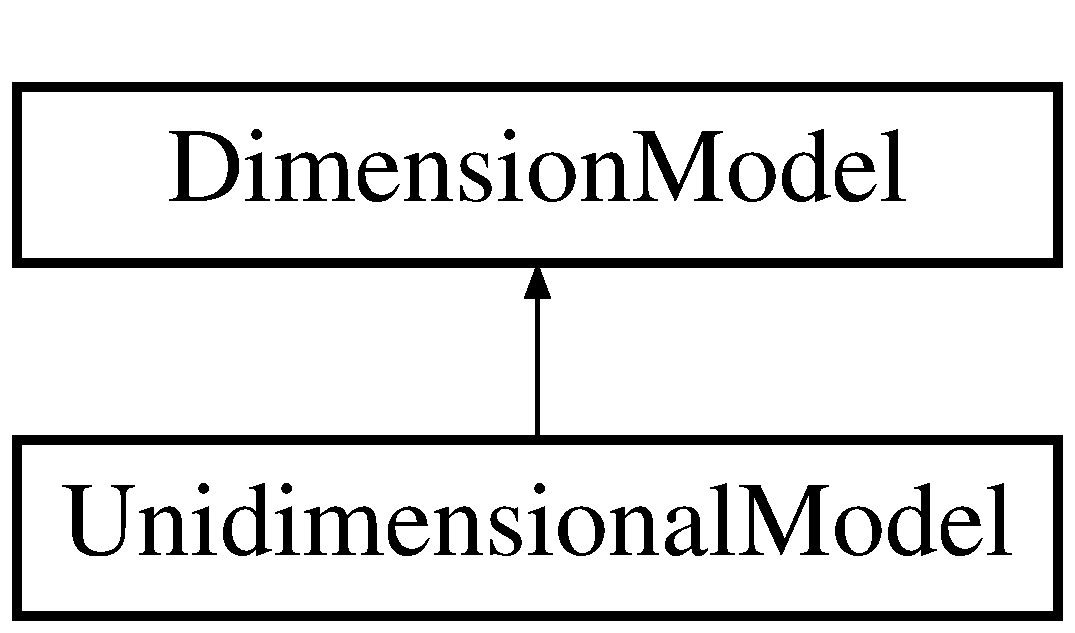
\includegraphics[height=2.000000cm]{classUnidimensionalModel}
\end{center}
\end{figure}
\subsection*{Public Member Functions}
\begin{DoxyCompactItemize}
\item 
\hyperlink{classUnidimensionalModel_a7687f3972c99830c87722b2503ad0c0b}{Unidimensional\+Model} ()
\item 
int \hyperlink{classUnidimensionalModel_a98a0a8d59c3b7d770579dba0a14f4802}{get\+Num\+Dimensions} ()
\item 
vector$<$ int $>$ \hyperlink{classUnidimensionalModel_a31d345c00b118a0c9efdc36592d4edd1}{get\+Dim\+Vector} ()
\item 
\hyperlink{classLatentTraitSet}{Latent\+Trait\+Set} $\ast$ \hyperlink{classUnidimensionalModel_a1876249eafaaa89b145c50adc8b4745a}{get\+Latent\+Trait\+Set} () const 
\item 
void \hyperlink{classUnidimensionalModel_ab71959d21ff63f9d2fc15cf6a815b408}{set\+Latent\+Trait\+Set} (\hyperlink{classLatentTraitSet}{Latent\+Trait\+Set} $\ast$\hyperlink{classDimensionModel_af202cd5a44ee99d865674c6e26d770c8}{latent\+Trait\+Set})
\item 
virtual \hyperlink{classUnidimensionalModel_aa3004b4f2f2840ffabe9c1628bb2cc3e}{$\sim$\+Unidimensional\+Model} ()
\end{DoxyCompactItemize}
\subsection*{Additional Inherited Members}


\subsection{Detailed Description}


Definition at line 13 of file Unidimensional\+Model.\+h.



\subsection{Constructor \& Destructor Documentation}
\hypertarget{classUnidimensionalModel_a7687f3972c99830c87722b2503ad0c0b}{}\index{Unidimensional\+Model@{Unidimensional\+Model}!Unidimensional\+Model@{Unidimensional\+Model}}
\index{Unidimensional\+Model@{Unidimensional\+Model}!Unidimensional\+Model@{Unidimensional\+Model}}
\subsubsection[{Unidimensional\+Model}]{\setlength{\rightskip}{0pt plus 5cm}Unidimensional\+Model\+::\+Unidimensional\+Model (
\begin{DoxyParamCaption}
{}
\end{DoxyParamCaption}
)}\label{classUnidimensionalModel_a7687f3972c99830c87722b2503ad0c0b}


Definition at line 10 of file Unidimensional\+Model.\+cpp.



References Dimension\+Model\+::latent\+Trait\+Set.

\hypertarget{classUnidimensionalModel_aa3004b4f2f2840ffabe9c1628bb2cc3e}{}\index{Unidimensional\+Model@{Unidimensional\+Model}!````~Unidimensional\+Model@{$\sim$\+Unidimensional\+Model}}
\index{````~Unidimensional\+Model@{$\sim$\+Unidimensional\+Model}!Unidimensional\+Model@{Unidimensional\+Model}}
\subsubsection[{$\sim$\+Unidimensional\+Model}]{\setlength{\rightskip}{0pt plus 5cm}Unidimensional\+Model\+::$\sim$\+Unidimensional\+Model (
\begin{DoxyParamCaption}
{}
\end{DoxyParamCaption}
)\hspace{0.3cm}{\ttfamily [virtual]}}\label{classUnidimensionalModel_aa3004b4f2f2840ffabe9c1628bb2cc3e}


Definition at line 35 of file Unidimensional\+Model.\+cpp.



References Dimension\+Model\+::latent\+Trait\+Set.



\subsection{Member Function Documentation}
\hypertarget{classUnidimensionalModel_a31d345c00b118a0c9efdc36592d4edd1}{}\index{Unidimensional\+Model@{Unidimensional\+Model}!get\+Dim\+Vector@{get\+Dim\+Vector}}
\index{get\+Dim\+Vector@{get\+Dim\+Vector}!Unidimensional\+Model@{Unidimensional\+Model}}
\subsubsection[{get\+Dim\+Vector}]{\setlength{\rightskip}{0pt plus 5cm}vector$<$ int $>$ Unidimensional\+Model\+::get\+Dim\+Vector (
\begin{DoxyParamCaption}
{}
\end{DoxyParamCaption}
)\hspace{0.3cm}{\ttfamily [virtual]}}\label{classUnidimensionalModel_a31d345c00b118a0c9efdc36592d4edd1}


Implements \hyperlink{classDimensionModel_a0aab2664f71949ac52d654730840056b}{Dimension\+Model}.



Definition at line 18 of file Unidimensional\+Model.\+cpp.



References Latent\+Trait\+Set\+::get\+Theta(), Dimension\+Model\+::latent\+Trait\+Set, and Matrix$<$ T $>$\+::n\+C().

\hypertarget{classUnidimensionalModel_a1876249eafaaa89b145c50adc8b4745a}{}\index{Unidimensional\+Model@{Unidimensional\+Model}!get\+Latent\+Trait\+Set@{get\+Latent\+Trait\+Set}}
\index{get\+Latent\+Trait\+Set@{get\+Latent\+Trait\+Set}!Unidimensional\+Model@{Unidimensional\+Model}}
\subsubsection[{get\+Latent\+Trait\+Set}]{\setlength{\rightskip}{0pt plus 5cm}{\bf Latent\+Trait\+Set} $\ast$ Unidimensional\+Model\+::get\+Latent\+Trait\+Set (
\begin{DoxyParamCaption}
{}
\end{DoxyParamCaption}
) const\hspace{0.3cm}{\ttfamily [virtual]}}\label{classUnidimensionalModel_a1876249eafaaa89b145c50adc8b4745a}


Implements \hyperlink{classDimensionModel_a37d2d9ab998a4e65628571e6144311f6}{Dimension\+Model}.



Definition at line 27 of file Unidimensional\+Model.\+cpp.



References Dimension\+Model\+::latent\+Trait\+Set.

\hypertarget{classUnidimensionalModel_a98a0a8d59c3b7d770579dba0a14f4802}{}\index{Unidimensional\+Model@{Unidimensional\+Model}!get\+Num\+Dimensions@{get\+Num\+Dimensions}}
\index{get\+Num\+Dimensions@{get\+Num\+Dimensions}!Unidimensional\+Model@{Unidimensional\+Model}}
\subsubsection[{get\+Num\+Dimensions}]{\setlength{\rightskip}{0pt plus 5cm}int Unidimensional\+Model\+::get\+Num\+Dimensions (
\begin{DoxyParamCaption}
{}
\end{DoxyParamCaption}
)\hspace{0.3cm}{\ttfamily [virtual]}}\label{classUnidimensionalModel_a98a0a8d59c3b7d770579dba0a14f4802}


Implements \hyperlink{classDimensionModel_aaf16c9215f4a7d08d67bd844adfcc62a}{Dimension\+Model}.



Definition at line 14 of file Unidimensional\+Model.\+cpp.

\hypertarget{classUnidimensionalModel_ab71959d21ff63f9d2fc15cf6a815b408}{}\index{Unidimensional\+Model@{Unidimensional\+Model}!set\+Latent\+Trait\+Set@{set\+Latent\+Trait\+Set}}
\index{set\+Latent\+Trait\+Set@{set\+Latent\+Trait\+Set}!Unidimensional\+Model@{Unidimensional\+Model}}
\subsubsection[{set\+Latent\+Trait\+Set}]{\setlength{\rightskip}{0pt plus 5cm}void Unidimensional\+Model\+::set\+Latent\+Trait\+Set (
\begin{DoxyParamCaption}
\item[{{\bf Latent\+Trait\+Set} $\ast$}]{latent\+Trait\+Set}
\end{DoxyParamCaption}
)\hspace{0.3cm}{\ttfamily [virtual]}}\label{classUnidimensionalModel_ab71959d21ff63f9d2fc15cf6a815b408}


Implements \hyperlink{classDimensionModel_aed42259f6cd663cbd1df07d18d4b1e07}{Dimension\+Model}.



Definition at line 31 of file Unidimensional\+Model.\+cpp.



References Dimension\+Model\+::latent\+Trait\+Set.



The documentation for this class was generated from the following files\+:\begin{DoxyCompactItemize}
\item 
src/model/dimension/\hyperlink{UnidimensionalModel_8h}{Unidimensional\+Model.\+h}\item 
src/model/dimension/\hyperlink{UnidimensionalModel_8cpp}{Unidimensional\+Model.\+cpp}\end{DoxyCompactItemize}

\chapter{File Documentation}
\hypertarget{BayesianEstimation_8cpp}{}\section{src/estimation/bayesian/\+Bayesian\+Estimation.cpp File Reference}
\label{BayesianEstimation_8cpp}\index{src/estimation/bayesian/\+Bayesian\+Estimation.\+cpp@{src/estimation/bayesian/\+Bayesian\+Estimation.\+cpp}}
{\ttfamily \#include \char`\"{}Bayesian\+Estimation.\+h\char`\"{}}\\*

\hypertarget{BayesianEstimation_8h}{}\section{src/estimation/bayesian/\+Bayesian\+Estimation.h File Reference}
\label{BayesianEstimation_8h}\index{src/estimation/bayesian/\+Bayesian\+Estimation.\+h@{src/estimation/bayesian/\+Bayesian\+Estimation.\+h}}
{\ttfamily \#include $<$estimation/\+Estimation.\+h$>$}\\*
\subsection*{Classes}
\begin{DoxyCompactItemize}
\item 
class \hyperlink{classBayesianEstimation}{Bayesian\+Estimation}
\begin{DoxyCompactList}\small\item\em \hyperlink{classEstimation}{Estimation} interface for bayesian methods, currently not implemented. \end{DoxyCompactList}\end{DoxyCompactItemize}

\hypertarget{ClassicalEstimation_8cpp}{}\section{src/estimation/classical/\+Classical\+Estimation.cpp File Reference}
\label{ClassicalEstimation_8cpp}\index{src/estimation/classical/\+Classical\+Estimation.\+cpp@{src/estimation/classical/\+Classical\+Estimation.\+cpp}}
{\ttfamily \#include \char`\"{}Classical\+Estimation.\+h\char`\"{}}\\*

\hypertarget{ClassicalEstimation_8h}{}\section{src/estimation/classical/\+Classical\+Estimation.h File Reference}
\label{ClassicalEstimation_8h}\index{src/estimation/classical/\+Classical\+Estimation.\+h@{src/estimation/classical/\+Classical\+Estimation.\+h}}
{\ttfamily \#include $<$estimation/\+Estimation.\+h$>$}\\*
\subsection*{Classes}
\begin{DoxyCompactItemize}
\item 
class \hyperlink{classClassicalEstimation}{Classical\+Estimation}
\begin{DoxyCompactList}\small\item\em Classical estimation class all the classical estimation methods must derive from this class this class is an interface. \end{DoxyCompactList}\end{DoxyCompactItemize}

\hypertarget{EMEstimation_8cpp}{}\section{src/estimation/classical/\+E\+M\+Estimation.cpp File Reference}
\label{EMEstimation_8cpp}\index{src/estimation/classical/\+E\+M\+Estimation.\+cpp@{src/estimation/classical/\+E\+M\+Estimation.\+cpp}}
{\ttfamily \#include \char`\"{}E\+M\+Estimation.\+h\char`\"{}}\\*

\hypertarget{EMEstimation_8h}{}\section{src/estimation/classical/\+E\+M\+Estimation.h File Reference}
\label{EMEstimation_8h}\index{src/estimation/classical/\+E\+M\+Estimation.\+h@{src/estimation/classical/\+E\+M\+Estimation.\+h}}
{\ttfamily \#include $<$estimation/classical/\+Classical\+Estimation.\+h$>$}\\*
{\ttfamily \#include $<$string$>$}\\*
{\ttfamily \#include $<$trace/\+Trace.\+h$>$}\\*
{\ttfamily \#include $<$type/\+Matrix.\+h$>$}\\*
{\ttfamily \#include $<$type/\+Pattern\+Matrix.\+h$>$}\\*
\subsection*{Classes}
\begin{DoxyCompactItemize}
\item 
class \hyperlink{classEMEstimation}{E\+M\+Estimation}
\begin{DoxyCompactList}\small\item\em Classical estimation through the E\+M algorithm, generic for the models however must be called with specific model object, the optimization algorithm can be any from the optimizers class. \end{DoxyCompactList}\end{DoxyCompactItemize}

\hypertarget{Estimation_8cpp}{}\section{src/estimation/\+Estimation.cpp File Reference}
\label{Estimation_8cpp}\index{src/estimation/\+Estimation.\+cpp@{src/estimation/\+Estimation.\+cpp}}
{\ttfamily \#include \char`\"{}Estimation.\+h\char`\"{}}\\*

\hypertarget{Estimation_8h}{}\section{src/estimation/\+Estimation.h File Reference}
\label{Estimation_8h}\index{src/estimation/\+Estimation.\+h@{src/estimation/\+Estimation.\+h}}
{\ttfamily \#include $<$model/\+Model.\+h$>$}\\*
{\ttfamily \#include $<$type/\+Matrix.\+h$>$}\\*
{\ttfamily \#include $<$optimizer/\+Optimizer.\+h$>$}\\*
{\ttfamily \#include $<$model/parameter/\+Three\+P\+L\+Model.\+h$>$}\\*
\subsection*{Classes}
\begin{DoxyCompactItemize}
\item 
class \hyperlink{classEstimation}{Estimation}
\begin{DoxyCompactList}\small\item\em Parent estimation interface for all estimation methods. \end{DoxyCompactList}\end{DoxyCompactItemize}

\hypertarget{Input_8cpp}{}\section{src/input/\+Input.cpp File Reference}
\label{Input_8cpp}\index{src/input/\+Input.\+cpp@{src/input/\+Input.\+cpp}}
{\ttfamily \#include \char`\"{}Input.\+h\char`\"{}}\\*

\hypertarget{Input_8h}{}\section{src/input/\+Input.h File Reference}
\label{Input_8h}\index{src/input/\+Input.\+h@{src/input/\+Input.\+h}}
{\ttfamily \#include $<$map$>$}\\*
{\ttfamily \#include $<$cstdio$>$}\\*
{\ttfamily \#include $<$cstring$>$}\\*
{\ttfamily \#include $<$string$>$}\\*
{\ttfamily \#include $<$cmath$>$}\\*
{\ttfamily \#include $<$iostream$>$}\\*
{\ttfamily \#include $<$ctype.\+h$>$}\\*
{\ttfamily \#include $<$fstream$>$}\\*
{\ttfamily \#include $<$type/\+Pattern\+Matrix.\+h$>$}\\*
{\ttfamily \#include $<$type/\+Matrix.\+h$>$}\\*
{\ttfamily \#include $<$trace/\+Trace.\+h$>$}\\*
\subsection*{Classes}
\begin{DoxyCompactItemize}
\item 
class \hyperlink{classInput}{Input}
\begin{DoxyCompactList}\small\item\em Class that is in charge of taking O\+S files, streams and other sources for inputting data into the software suite. \end{DoxyCompactList}\end{DoxyCompactItemize}

\hypertarget{Main_8cpp}{}\section{src/main/\+Main.cpp File Reference}
\label{Main_8cpp}\index{src/main/\+Main.\+cpp@{src/main/\+Main.\+cpp}}
{\ttfamily \#include \char`\"{}Main.\+h\char`\"{}}\\*
\subsection*{Functions}
\begin{DoxyCompactItemize}
\item 
double \hyperlink{Main_8cpp_af99bd234e9c85ddacb1e4c723821438b}{banana} (double $\ast$args, double $\ast$pars, int nargs, int npars)
\item 
void \hyperlink{Main_8cpp_a1b63faa35546b1036d44672e30c95ac8}{banana\+Gradient} (double $\ast$args, double $\ast$pars, int nargs, int npars, double $\ast$\hyperlink{NCM_8h_af15a746b92f8a980c82fa216ce598faf}{gradient})
\item 
void \hyperlink{Main_8cpp_ad28b108bb1686262e8db88fa1f6e473b}{rosenbrock\+Test} ()
\item 
void \hyperlink{Main_8cpp_ac0b46a7748d663983a97334ea7851455}{pachotest} ()
\item 
void \hyperlink{Main_8cpp_a06800f4745a82946a3e8e740f6bbd15f}{init\+Tests} (char $\ast$filename)
\item 
void \hyperlink{Main_8cpp_a22339de75a9aeeffd35c9c0cfd7a2848}{one\+Run} ()
\item 
int \hyperlink{Main_8cpp_a0ddf1224851353fc92bfbff6f499fa97}{main} (int argc, char $\ast$argv\mbox{[}$\,$\mbox{]})
\end{DoxyCompactItemize}


\subsection{Function Documentation}
\hypertarget{Main_8cpp_af99bd234e9c85ddacb1e4c723821438b}{}\index{Main.\+cpp@{Main.\+cpp}!banana@{banana}}
\index{banana@{banana}!Main.\+cpp@{Main.\+cpp}}
\subsubsection[{banana}]{\setlength{\rightskip}{0pt plus 5cm}double banana (
\begin{DoxyParamCaption}
\item[{double $\ast$}]{args, }
\item[{double $\ast$}]{pars, }
\item[{int}]{nargs, }
\item[{int}]{npars}
\end{DoxyParamCaption}
)}\label{Main_8cpp_af99bd234e9c85ddacb1e4c723821438b}


Definition at line 14 of file Main.\+cpp.



Referenced by banana\+Gradient(), and rosenbrock\+Test().

\hypertarget{Main_8cpp_a1b63faa35546b1036d44672e30c95ac8}{}\index{Main.\+cpp@{Main.\+cpp}!banana\+Gradient@{banana\+Gradient}}
\index{banana\+Gradient@{banana\+Gradient}!Main.\+cpp@{Main.\+cpp}}
\subsubsection[{banana\+Gradient}]{\setlength{\rightskip}{0pt plus 5cm}void banana\+Gradient (
\begin{DoxyParamCaption}
\item[{double $\ast$}]{args, }
\item[{double $\ast$}]{pars, }
\item[{int}]{nargs, }
\item[{int}]{npars, }
\item[{double $\ast$}]{gradient}
\end{DoxyParamCaption}
)}\label{Main_8cpp_a1b63faa35546b1036d44672e30c95ac8}


Definition at line 21 of file Main.\+cpp.



References banana().



Referenced by rosenbrock\+Test().

\hypertarget{Main_8cpp_a06800f4745a82946a3e8e740f6bbd15f}{}\index{Main.\+cpp@{Main.\+cpp}!init\+Tests@{init\+Tests}}
\index{init\+Tests@{init\+Tests}!Main.\+cpp@{Main.\+cpp}}
\subsubsection[{init\+Tests}]{\setlength{\rightskip}{0pt plus 5cm}void init\+Tests (
\begin{DoxyParamCaption}
\item[{char $\ast$}]{filename}
\end{DoxyParamCaption}
)}\label{Main_8cpp_a06800f4745a82946a3e8e740f6bbd15f}


Definition at line 76 of file Main.\+cpp.



Referenced by main().

\hypertarget{Main_8cpp_a0ddf1224851353fc92bfbff6f499fa97}{}\index{Main.\+cpp@{Main.\+cpp}!main@{main}}
\index{main@{main}!Main.\+cpp@{Main.\+cpp}}
\subsubsection[{main}]{\setlength{\rightskip}{0pt plus 5cm}int main (
\begin{DoxyParamCaption}
\item[{int}]{argc, }
\item[{char $\ast$}]{argv\mbox{[}$\,$\mbox{]}}
\end{DoxyParamCaption}
)}\label{Main_8cpp_a0ddf1224851353fc92bfbff6f499fa97}


Definition at line 159 of file Main.\+cpp.



References init\+Tests().

\hypertarget{Main_8cpp_a22339de75a9aeeffd35c9c0cfd7a2848}{}\index{Main.\+cpp@{Main.\+cpp}!one\+Run@{one\+Run}}
\index{one\+Run@{one\+Run}!Main.\+cpp@{Main.\+cpp}}
\subsubsection[{one\+Run}]{\setlength{\rightskip}{0pt plus 5cm}void one\+Run (
\begin{DoxyParamCaption}
{}
\end{DoxyParamCaption}
)}\label{Main_8cpp_a22339de75a9aeeffd35c9c0cfd7a2848}


Definition at line 84 of file Main.\+cpp.



References a, Parameter\+Model\+::build\+Parameter\+Set(), c, Item\+Model\+::count\+Items(), d, E\+M\+Estimation\+::estimate(), Model\+::get\+Dimension\+Model(), Model\+::get\+Item\+Model(), Dimension\+Model\+::get\+Latent\+Trait\+Set(), Model\+::get\+Parameter\+Model(), Parameter\+Model\+::get\+Parameter\+Set(), Input\+::import\+C\+S\+V(), Matrix$<$ T $>$\+::n\+R(), Item\+Model\+::set\+Dataset(), Model\+::set\+Model(), E\+M\+Estimation\+::set\+Model(), Latent\+Trait\+Set\+::set\+Theta(), and Latent\+Trait\+Set\+::set\+Weight().

\hypertarget{Main_8cpp_ac0b46a7748d663983a97334ea7851455}{}\index{Main.\+cpp@{Main.\+cpp}!pachotest@{pachotest}}
\index{pachotest@{pachotest}!Main.\+cpp@{Main.\+cpp}}
\subsubsection[{pachotest}]{\setlength{\rightskip}{0pt plus 5cm}void pachotest (
\begin{DoxyParamCaption}
{}
\end{DoxyParamCaption}
)}\label{Main_8cpp_ac0b46a7748d663983a97334ea7851455}


Definition at line 69 of file Main.\+cpp.



References Approximate\+Matrix\+Inverse(), and Input\+::import\+C\+S\+V().

\hypertarget{Main_8cpp_ad28b108bb1686262e8db88fa1f6e473b}{}\index{Main.\+cpp@{Main.\+cpp}!rosenbrock\+Test@{rosenbrock\+Test}}
\index{rosenbrock\+Test@{rosenbrock\+Test}!Main.\+cpp@{Main.\+cpp}}
\subsubsection[{rosenbrock\+Test}]{\setlength{\rightskip}{0pt plus 5cm}void rosenbrock\+Test (
\begin{DoxyParamCaption}
{}
\end{DoxyParamCaption}
)}\label{Main_8cpp_ad28b108bb1686262e8db88fa1f6e473b}


Definition at line 33 of file Main.\+cpp.



References banana(), banana\+Gradient(), gradient(), and Optimizer\+::search\+Optimal().


\hypertarget{Main_8h}{}\section{src/main/\+Main.h File Reference}
\label{Main_8h}\index{src/main/\+Main.\+h@{src/main/\+Main.\+h}}
{\ttfamily \#include $<$iostream$>$}\\*
{\ttfamily \#include $<$type/\+Matrix.\+h$>$}\\*
{\ttfamily \#include $<$boost/dynamic\+\_\+bitset.\+hpp$>$}\\*
{\ttfamily \#include $<$type/\+Pattern\+Matrix.\+h$>$}\\*
{\ttfamily \#include $<$model/\+Model.\+h$>$}\\*
{\ttfamily \#include $<$model/\+Model\+Factory.\+h$>$}\\*
{\ttfamily \#include $<$model/\+S\+I\+C\+S\+General\+Model.\+h$>$}\\*
{\ttfamily \#include $<$estimation/classical/\+E\+M\+Estimation.\+h$>$}\\*
{\ttfamily \#include $<$input/\+Input.\+h$>$}\\*
{\ttfamily \#include $<$util/\+N\+C\+M.\+h$>$}\\*
{\ttfamily \#include \char`\"{}util/blas\+Interface.\+h\char`\"{}}\\*
{\ttfamily \#include $<$../test/\+E\+M\+Test.\+h$>$}\\*

\hypertarget{DimensionModel_8cpp}{}\section{src/model/dimension/\+Dimension\+Model.cpp File Reference}
\label{DimensionModel_8cpp}\index{src/model/dimension/\+Dimension\+Model.\+cpp@{src/model/dimension/\+Dimension\+Model.\+cpp}}
{\ttfamily \#include $<$model/dimension/\+Dimension\+Model.\+h$>$}\\*

\hypertarget{DimensionModel_8h}{}\section{src/model/dimension/\+Dimension\+Model.h File Reference}
\label{DimensionModel_8h}\index{src/model/dimension/\+Dimension\+Model.\+h@{src/model/dimension/\+Dimension\+Model.\+h}}
{\ttfamily \#include $<$vector$>$}\\*
{\ttfamily \#include $<$type/\+Latent\+Trait\+Set.\+h$>$}\\*
\subsection*{Classes}
\begin{DoxyCompactItemize}
\item 
class \hyperlink{classDimensionModel}{Dimension\+Model}
\end{DoxyCompactItemize}

\hypertarget{MultidimensionalModel_8cpp}{}\section{src/model/dimension/\+Multidimensional\+Model.cpp File Reference}
\label{MultidimensionalModel_8cpp}\index{src/model/dimension/\+Multidimensional\+Model.\+cpp@{src/model/dimension/\+Multidimensional\+Model.\+cpp}}
{\ttfamily \#include \char`\"{}Multidimensional\+Model.\+h\char`\"{}}\\*

\hypertarget{MultidimensionalModel_8h}{}\section{src/model/dimension/\+Multidimensional\+Model.h File Reference}
\label{MultidimensionalModel_8h}\index{src/model/dimension/\+Multidimensional\+Model.\+h@{src/model/dimension/\+Multidimensional\+Model.\+h}}
{\ttfamily \#include $<$vector$>$}\\*
{\ttfamily \#include $<$type/\+Latent\+Trait\+Set.\+h$>$}\\*
{\ttfamily \#include $<$model/dimension/\+Dimension\+Model.\+h$>$}\\*
\subsection*{Classes}
\begin{DoxyCompactItemize}
\item 
class \hyperlink{classMultidimensionalModel}{Multidimensional\+Model}
\end{DoxyCompactItemize}

\hypertarget{MultiUniDimModel_8cpp}{}\section{src/model/dimension/\+Multi\+Uni\+Dim\+Model.cpp File Reference}
\label{MultiUniDimModel_8cpp}\index{src/model/dimension/\+Multi\+Uni\+Dim\+Model.\+cpp@{src/model/dimension/\+Multi\+Uni\+Dim\+Model.\+cpp}}
{\ttfamily \#include $<$model/dimension/\+Multi\+Uni\+Dim\+Model.\+h$>$}\\*

\hypertarget{MultiUniDimModel_8h}{}\section{src/model/dimension/\+Multi\+Uni\+Dim\+Model.h File Reference}
\label{MultiUniDimModel_8h}\index{src/model/dimension/\+Multi\+Uni\+Dim\+Model.\+h@{src/model/dimension/\+Multi\+Uni\+Dim\+Model.\+h}}
{\ttfamily \#include $<$model/dimension/\+Dimension\+Model.\+h$>$}\\*
\subsection*{Classes}
\begin{DoxyCompactItemize}
\item 
class \hyperlink{classMultiUniDimModel}{Multi\+Uni\+Dim\+Model}
\end{DoxyCompactItemize}

\hypertarget{UnidimensionalModel_8cpp}{}\section{src/model/dimension/\+Unidimensional\+Model.cpp File Reference}
\label{UnidimensionalModel_8cpp}\index{src/model/dimension/\+Unidimensional\+Model.\+cpp@{src/model/dimension/\+Unidimensional\+Model.\+cpp}}
{\ttfamily \#include $<$model/dimension/\+Unidimensional\+Model.\+h$>$}\\*

\hypertarget{UnidimensionalModel_8h}{}\section{src/model/dimension/\+Unidimensional\+Model.h File Reference}
\label{UnidimensionalModel_8h}\index{src/model/dimension/\+Unidimensional\+Model.\+h@{src/model/dimension/\+Unidimensional\+Model.\+h}}
{\ttfamily \#include $<$model/dimension/\+Dimension\+Model.\+h$>$}\\*
\subsection*{Classes}
\begin{DoxyCompactItemize}
\item 
class \hyperlink{classUnidimensionalModel}{Unidimensional\+Model}
\end{DoxyCompactItemize}

\hypertarget{DichotomousModel_8cpp}{}\section{src/model/item/\+Dichotomous\+Model.cpp File Reference}
\label{DichotomousModel_8cpp}\index{src/model/item/\+Dichotomous\+Model.\+cpp@{src/model/item/\+Dichotomous\+Model.\+cpp}}
{\ttfamily \#include $<$model/item/\+Dichotomous\+Model.\+h$>$}\\*

\hypertarget{DichotomousModel_8h}{}\section{src/model/item/\+Dichotomous\+Model.h File Reference}
\label{DichotomousModel_8h}\index{src/model/item/\+Dichotomous\+Model.\+h@{src/model/item/\+Dichotomous\+Model.\+h}}
{\ttfamily \#include $<$model/item/\+Item\+Model.\+h$>$}\\*
{\ttfamily \#include $<$type/\+Pattern\+Matrix.\+h$>$}\\*
\subsection*{Classes}
\begin{DoxyCompactItemize}
\item 
class \hyperlink{classDichotomousModel}{Dichotomous\+Model}
\end{DoxyCompactItemize}

\hypertarget{ItemModel_8cpp}{}\section{src/model/item/\+Item\+Model.cpp File Reference}
\label{ItemModel_8cpp}\index{src/model/item/\+Item\+Model.\+cpp@{src/model/item/\+Item\+Model.\+cpp}}
{\ttfamily \#include $<$model/item/\+Item\+Model.\+h$>$}\\*

\hypertarget{ItemModel_8h}{}\section{src/model/item/\+Item\+Model.h File Reference}
\label{ItemModel_8h}\index{src/model/item/\+Item\+Model.\+h@{src/model/item/\+Item\+Model.\+h}}
{\ttfamily \#include $<$type/\+Data\+Set.\+h$>$}\\*
\subsection*{Classes}
\begin{DoxyCompactItemize}
\item 
class \hyperlink{classItemModel}{Item\+Model}
\end{DoxyCompactItemize}

\hypertarget{PolytomousModel_8cpp}{}\section{src/model/item/\+Polytomous\+Model.cpp File Reference}
\label{PolytomousModel_8cpp}\index{src/model/item/\+Polytomous\+Model.\+cpp@{src/model/item/\+Polytomous\+Model.\+cpp}}
{\ttfamily \#include $<$model/item/\+Polytomous\+Model.\+h$>$}\\*

\hypertarget{PolytomousModel_8h}{}\section{src/model/item/\+Polytomous\+Model.h File Reference}
\label{PolytomousModel_8h}\index{src/model/item/\+Polytomous\+Model.\+h@{src/model/item/\+Polytomous\+Model.\+h}}
{\ttfamily \#include $<$model/item/\+Item\+Model.\+h$>$}\\*
\subsection*{Classes}
\begin{DoxyCompactItemize}
\item 
class \hyperlink{classPolytomousModel}{Polytomous\+Model}
\end{DoxyCompactItemize}

\hypertarget{Model_8cpp}{}\section{src/model/\+Model.cpp File Reference}
\label{Model_8cpp}\index{src/model/\+Model.\+cpp@{src/model/\+Model.\+cpp}}
{\ttfamily \#include \char`\"{}Model.\+h\char`\"{}}\\*

\hypertarget{Model_8h}{}\section{src/model/\+Model.h File Reference}
\label{Model_8h}\index{src/model/\+Model.\+h@{src/model/\+Model.\+h}}
{\ttfamily \#include $<$model/parameter/\+Parameter\+Model.\+h$>$}\\*
{\ttfamily \#include $<$model/item/\+Item\+Model.\+h$>$}\\*
{\ttfamily \#include $<$model/dimension/\+Dimension\+Model.\+h$>$}\\*
{\ttfamily \#include $<$model/\+Model\+Factory.\+h$>$}\\*
\subsection*{Classes}
\begin{DoxyCompactItemize}
\item 
class \hyperlink{classModel}{Model}
\begin{DoxyCompactList}\small\item\em \hyperlink{classModel}{Model} class that holds the structures for the I\+R\+T models can vary across parameters, items and dimensions includes suport for dichotomic and polytomic models multi and single dimensional models future suport for multiscale and longitudinal models can be implemented. \end{DoxyCompactList}\end{DoxyCompactItemize}

\hypertarget{ModelFactory_8cpp}{}\section{src/model/\+Model\+Factory.cpp File Reference}
\label{ModelFactory_8cpp}\index{src/model/\+Model\+Factory.\+cpp@{src/model/\+Model\+Factory.\+cpp}}
{\ttfamily \#include $<$model/\+Model\+Factory.\+h$>$}\\*

\hypertarget{ModelFactory_8h}{}\section{src/model/\+Model\+Factory.h File Reference}
\label{ModelFactory_8h}\index{src/model/\+Model\+Factory.\+h@{src/model/\+Model\+Factory.\+h}}
{\ttfamily \#include $<$model/parameter/\+Parameter\+Model.\+h$>$}\\*
{\ttfamily \#include $<$model/item/\+Item\+Model.\+h$>$}\\*
{\ttfamily \#include $<$model/dimension/\+Dimension\+Model.\+h$>$}\\*
\subsection*{Classes}
\begin{DoxyCompactItemize}
\item 
class \hyperlink{classModelFactory}{Model\+Factory}
\end{DoxyCompactItemize}

\hypertarget{ParameterModel_8cpp}{}\section{src/model/parameter/\+Parameter\+Model.cpp File Reference}
\label{ParameterModel_8cpp}\index{src/model/parameter/\+Parameter\+Model.\+cpp@{src/model/parameter/\+Parameter\+Model.\+cpp}}
{\ttfamily \#include $<$model/parameter/\+Parameter\+Model.\+h$>$}\\*

\hypertarget{ParameterModel_8h}{}\section{src/model/parameter/\+Parameter\+Model.h File Reference}
\label{ParameterModel_8h}\index{src/model/parameter/\+Parameter\+Model.\+h@{src/model/parameter/\+Parameter\+Model.\+h}}
{\ttfamily \#include $<$map$>$}\\*
{\ttfamily \#include $<$type/\+Matrix.\+h$>$}\\*
{\ttfamily \#include $<$model/item/\+Item\+Model.\+h$>$}\\*
{\ttfamily \#include $<$model/dimension/\+Dimension\+Model.\+h$>$}\\*
{\ttfamily \#include $<$type/\+Data\+Set.\+h$>$}\\*
\subsection*{Classes}
\begin{DoxyCompactItemize}
\item 
class \hyperlink{classParameterModel}{Parameter\+Model}
\end{DoxyCompactItemize}
\subsection*{Enumerations}
\begin{DoxyCompactItemize}
\item 
enum \hyperlink{ParameterModel_8h_a04ed5b8f1f3adf7af1d5092fae847e90}{Parameter} \{ \hyperlink{ParameterModel_8h_a04ed5b8f1f3adf7af1d5092fae847e90aa91fb0824da12f8bb3b74dd78fb13b63}{a}, 
\hyperlink{ParameterModel_8h_a04ed5b8f1f3adf7af1d5092fae847e90aa06b03e4cd5c7c464c513a95a7fcf9bf}{b}, 
\hyperlink{ParameterModel_8h_a04ed5b8f1f3adf7af1d5092fae847e90a776304400122408ea717dde9234fdd2a}{c}, 
\hyperlink{ParameterModel_8h_a04ed5b8f1f3adf7af1d5092fae847e90ae8f0ad1953249e38043d318b8f4400d0}{d}
 \}
\end{DoxyCompactItemize}


\subsection{Enumeration Type Documentation}
\hypertarget{ParameterModel_8h_a04ed5b8f1f3adf7af1d5092fae847e90}{}\index{Parameter\+Model.\+h@{Parameter\+Model.\+h}!Parameter@{Parameter}}
\index{Parameter@{Parameter}!Parameter\+Model.\+h@{Parameter\+Model.\+h}}
\subsubsection[{Parameter}]{\setlength{\rightskip}{0pt plus 5cm}enum {\bf Parameter}}\label{ParameterModel_8h_a04ed5b8f1f3adf7af1d5092fae847e90}
\begin{Desc}
\item[Enumerator]\par
\begin{description}
\index{a@{a}!Parameter\+Model.\+h@{Parameter\+Model.\+h}}\index{Parameter\+Model.\+h@{Parameter\+Model.\+h}!a@{a}}\item[{\em 
\hypertarget{ParameterModel_8h_a04ed5b8f1f3adf7af1d5092fae847e90aa91fb0824da12f8bb3b74dd78fb13b63}{}a\label{ParameterModel_8h_a04ed5b8f1f3adf7af1d5092fae847e90aa91fb0824da12f8bb3b74dd78fb13b63}
}]\index{b@{b}!Parameter\+Model.\+h@{Parameter\+Model.\+h}}\index{Parameter\+Model.\+h@{Parameter\+Model.\+h}!b@{b}}\item[{\em 
\hypertarget{ParameterModel_8h_a04ed5b8f1f3adf7af1d5092fae847e90aa06b03e4cd5c7c464c513a95a7fcf9bf}{}b\label{ParameterModel_8h_a04ed5b8f1f3adf7af1d5092fae847e90aa06b03e4cd5c7c464c513a95a7fcf9bf}
}]\index{c@{c}!Parameter\+Model.\+h@{Parameter\+Model.\+h}}\index{Parameter\+Model.\+h@{Parameter\+Model.\+h}!c@{c}}\item[{\em 
\hypertarget{ParameterModel_8h_a04ed5b8f1f3adf7af1d5092fae847e90a776304400122408ea717dde9234fdd2a}{}c\label{ParameterModel_8h_a04ed5b8f1f3adf7af1d5092fae847e90a776304400122408ea717dde9234fdd2a}
}]\index{d@{d}!Parameter\+Model.\+h@{Parameter\+Model.\+h}}\index{Parameter\+Model.\+h@{Parameter\+Model.\+h}!d@{d}}\item[{\em 
\hypertarget{ParameterModel_8h_a04ed5b8f1f3adf7af1d5092fae847e90ae8f0ad1953249e38043d318b8f4400d0}{}d\label{ParameterModel_8h_a04ed5b8f1f3adf7af1d5092fae847e90ae8f0ad1953249e38043d318b8f4400d0}
}]\end{description}
\end{Desc}


Definition at line 19 of file Parameter\+Model.\+h.


\hypertarget{RaschModel_8cpp}{}\section{src/model/parameter/\+Rasch\+Model.cpp File Reference}
\label{RaschModel_8cpp}\index{src/model/parameter/\+Rasch\+Model.\+cpp@{src/model/parameter/\+Rasch\+Model.\+cpp}}
{\ttfamily \#include $<$model/parameter/\+Rasch\+Model.\+h$>$}\\*

\hypertarget{RaschModel_8h}{}\section{src/model/parameter/\+Rasch\+Model.h File Reference}
\label{RaschModel_8h}\index{src/model/parameter/\+Rasch\+Model.\+h@{src/model/parameter/\+Rasch\+Model.\+h}}
{\ttfamily \#include $<$model/parameter/\+Parameter\+Model.\+h$>$}\\*
\subsection*{Classes}
\begin{DoxyCompactItemize}
\item 
class \hyperlink{classRaschModel}{Rasch\+Model}
\end{DoxyCompactItemize}

\hypertarget{ThreePLModel_8cpp}{}\section{src/model/parameter/\+Three\+P\+L\+Model.cpp File Reference}
\label{ThreePLModel_8cpp}\index{src/model/parameter/\+Three\+P\+L\+Model.\+cpp@{src/model/parameter/\+Three\+P\+L\+Model.\+cpp}}
{\ttfamily \#include $<$model/parameter/\+Three\+P\+L\+Model.\+h$>$}\\*

\hypertarget{ThreePLModel_8h}{}\section{src/model/parameter/\+Three\+P\+L\+Model.h File Reference}
\label{ThreePLModel_8h}\index{src/model/parameter/\+Three\+P\+L\+Model.\+h@{src/model/parameter/\+Three\+P\+L\+Model.\+h}}
{\ttfamily \#include $<$typeinfo$>$}\\*
{\ttfamily \#include $<$model/parameter/\+Parameter\+Model.\+h$>$}\\*
{\ttfamily \#include $<$model/item/\+Dichotomous\+Model.\+h$>$}\\*
{\ttfamily \#include $<$model/item/\+Polytomous\+Model.\+h$>$}\\*
{\ttfamily \#include $<$model/dimension/\+Unidimensional\+Model.\+h$>$}\\*
{\ttfamily \#include $<$model/dimension/\+Multidimensional\+Model.\+h$>$}\\*
{\ttfamily \#include $<$model/dimension/\+Multi\+Uni\+Dim\+Model.\+h$>$}\\*
{\ttfamily \#include $<$type/\+Pattern\+Matrix.\+h$>$}\\*
{\ttfamily \#include $<$type/\+Constant.\+h$>$}\\*
{\ttfamily \#include $<$cmath$>$}\\*
\subsection*{Classes}
\begin{DoxyCompactItemize}
\item 
class \hyperlink{classThreePLModel}{Three\+P\+L\+Model}
\begin{DoxyCompactList}\small\item\em \hyperlink{classModel}{Model} for the 3pl model, uses parameters a d c. \end{DoxyCompactList}\end{DoxyCompactItemize}

\hypertarget{TwoPLModel_8cpp}{}\section{src/model/parameter/\+Two\+P\+L\+Model.cpp File Reference}
\label{TwoPLModel_8cpp}\index{src/model/parameter/\+Two\+P\+L\+Model.\+cpp@{src/model/parameter/\+Two\+P\+L\+Model.\+cpp}}
{\ttfamily \#include $<$model/parameter/\+Two\+P\+L\+Model.\+h$>$}\\*

\hypertarget{TwoPLModel_8h}{}\section{src/model/parameter/\+Two\+P\+L\+Model.h File Reference}
\label{TwoPLModel_8h}\index{src/model/parameter/\+Two\+P\+L\+Model.\+h@{src/model/parameter/\+Two\+P\+L\+Model.\+h}}
{\ttfamily \#include $<$model/parameter/\+Parameter\+Model.\+h$>$}\\*
\subsection*{Classes}
\begin{DoxyCompactItemize}
\item 
class \hyperlink{classTwoPLModel}{Two\+P\+L\+Model}
\end{DoxyCompactItemize}

\hypertarget{SICSGeneralModel_8cpp}{}\section{src/model/\+S\+I\+C\+S\+General\+Model.cpp File Reference}
\label{SICSGeneralModel_8cpp}\index{src/model/\+S\+I\+C\+S\+General\+Model.\+cpp@{src/model/\+S\+I\+C\+S\+General\+Model.\+cpp}}
{\ttfamily \#include $<$model/\+S\+I\+C\+S\+General\+Model.\+h$>$}\\*

\hypertarget{SICSGeneralModel_8h}{}\section{src/model/\+S\+I\+C\+S\+General\+Model.h File Reference}
\label{SICSGeneralModel_8h}\index{src/model/\+S\+I\+C\+S\+General\+Model.\+h@{src/model/\+S\+I\+C\+S\+General\+Model.\+h}}
{\ttfamily \#include $<$model/\+Model\+Factory.\+h$>$}\\*
{\ttfamily \#include $<$model/parameter/\+Three\+P\+L\+Model.\+h$>$}\\*
{\ttfamily \#include $<$model/item/\+Dichotomous\+Model.\+h$>$}\\*
{\ttfamily \#include $<$model/dimension/\+Unidimensional\+Model.\+h$>$}\\*
\subsection*{Classes}
\begin{DoxyCompactItemize}
\item 
class \hyperlink{classSICSGeneralModel}{S\+I\+C\+S\+General\+Model}
\end{DoxyCompactItemize}

\hypertarget{BFGSOptimizer_8h}{}\section{src/optimizer/\+B\+F\+G\+S\+Optimizer.h File Reference}
\label{BFGSOptimizer_8h}\index{src/optimizer/\+B\+F\+G\+S\+Optimizer.\+h@{src/optimizer/\+B\+F\+G\+S\+Optimizer.\+h}}
{\ttfamily \#include $<$type/\+Constant.\+h$>$}\\*
{\ttfamily \#include $<$cmath$>$}\\*
{\ttfamily \#include $<$stdlib.\+h$>$}\\*
{\ttfamily \#include $<$iostream$>$}\\*

\hypertarget{FisherScoringOptimizer_8h}{}\section{src/optimizer/\+Fisher\+Scoring\+Optimizer.h File Reference}
\label{FisherScoringOptimizer_8h}\index{src/optimizer/\+Fisher\+Scoring\+Optimizer.\+h@{src/optimizer/\+Fisher\+Scoring\+Optimizer.\+h}}
\subsection*{Classes}
\begin{DoxyCompactItemize}
\item 
class \hyperlink{classFisherScoringOptimizer}{Fisher\+Scoring\+Optimizer}
\begin{DoxyCompactList}\small\item\em Skeleton for implementing the Fisher \hyperlink{classOptimizer}{Optimizer}. \end{DoxyCompactList}\end{DoxyCompactItemize}

\hypertarget{NewtonOptimizer_8h}{}\section{src/optimizer/\+Newton\+Optimizer.h File Reference}
\label{NewtonOptimizer_8h}\index{src/optimizer/\+Newton\+Optimizer.\+h@{src/optimizer/\+Newton\+Optimizer.\+h}}
{\ttfamily \#include $<$math.\+h$>$}\\*
{\ttfamily \#include $<$type/\+Matrix.\+h$>$}\\*
{\ttfamily \#include $<$util/blas\+Interface.\+h$>$}\\*

\hypertarget{Optimizer_8cpp}{}\section{src/optimizer/\+Optimizer.cpp File Reference}
\label{Optimizer_8cpp}\index{src/optimizer/\+Optimizer.\+cpp@{src/optimizer/\+Optimizer.\+cpp}}
{\ttfamily \#include $<$optimizer/\+Optimizer.\+h$>$}\\*

\hypertarget{Optimizer_8h}{}\section{src/optimizer/\+Optimizer.h File Reference}
\label{Optimizer_8h}\index{src/optimizer/\+Optimizer.\+h@{src/optimizer/\+Optimizer.\+h}}
{\ttfamily \#include $<$optimizer/\+Newton\+Optimizer.\+h$>$}\\*
{\ttfamily \#include $<$optimizer/\+Fisher\+Scoring\+Optimizer.\+h$>$}\\*
{\ttfamily \#include $<$optimizer/\+B\+F\+G\+S\+Optimizer.\+h$>$}\\*
\subsection*{Classes}
\begin{DoxyCompactItemize}
\item 
class \hyperlink{classOptimizer}{Optimizer}
\begin{DoxyCompactList}\small\item\em Wrapper for the other optimizers, take general functions for the function to optimize, the vector gradient function and the matrix hessian function The parameters are \+: double $\ast$ args (Arguments over which the function optimizes) double $\ast$ pars (Arguments in whose the function depends but are not optimized) int nargs Number of arguments int npars Number of parameters double $\ast$ return (Return of the function is put in this array.) \end{DoxyCompactList}\end{DoxyCompactItemize}

\hypertarget{Output_8cpp}{}\section{src/output/\+Output.cpp File Reference}
\label{Output_8cpp}\index{src/output/\+Output.\+cpp@{src/output/\+Output.\+cpp}}
{\ttfamily \#include \char`\"{}Output.\+h\char`\"{}}\\*

\hypertarget{Output_8h}{}\section{src/output/\+Output.h File Reference}
\label{Output_8h}\index{src/output/\+Output.\+h@{src/output/\+Output.\+h}}
\subsection*{Classes}
\begin{DoxyCompactItemize}
\item 
class \hyperlink{classOutput}{Output}
\begin{DoxyCompactList}\small\item\em Skeleton for the output class T\+O\+D\+O \+: C\+S\+V output T\+O\+D\+O \+: J\+S\+O\+N online output T\+O\+D\+O \+: Te\+X output for reports. \end{DoxyCompactList}\end{DoxyCompactItemize}

\hypertarget{Trace_8cpp}{}\section{src/trace/\+Trace.cpp File Reference}
\label{Trace_8cpp}\index{src/trace/\+Trace.\+cpp@{src/trace/\+Trace.\+cpp}}
{\ttfamily \#include \char`\"{}Trace.\+h\char`\"{}}\\*

\hypertarget{Trace_8h}{}\section{src/trace/\+Trace.h File Reference}
\label{Trace_8h}\index{src/trace/\+Trace.\+h@{src/trace/\+Trace.\+h}}
{\ttfamily \#include $<$string$>$}\\*
{\ttfamily \#include $<$fstream$>$}\\*
{\ttfamily \#include $<$type/\+Matrix.\+h$>$}\\*
\subsection*{Classes}
\begin{DoxyCompactItemize}
\item 
class \hyperlink{classTrace}{Trace}
\begin{DoxyCompactList}\small\item\em \hyperlink{classTrace}{Trace} class for constructing execution and error logs onto files. \end{DoxyCompactList}\end{DoxyCompactItemize}

\hypertarget{Argument_8cpp}{}\section{src/type/\+Argument.cpp File Reference}
\label{Argument_8cpp}\index{src/type/\+Argument.\+cpp@{src/type/\+Argument.\+cpp}}
{\ttfamily \#include $<$type/\+Argument.\+h$>$}\\*

\hypertarget{Argument_8h}{}\section{src/type/\+Argument.h File Reference}
\label{Argument_8h}\index{src/type/\+Argument.\+h@{src/type/\+Argument.\+h}}
\subsection*{Classes}
\begin{DoxyCompactItemize}
\item 
class \hyperlink{classArgument}{Argument}
\end{DoxyCompactItemize}

\hypertarget{Constant_8cpp}{}\section{src/type/\+Constant.cpp File Reference}
\label{Constant_8cpp}\index{src/type/\+Constant.\+cpp@{src/type/\+Constant.\+cpp}}
{\ttfamily \#include $<$type/\+Constant.\+h$>$}\\*

\hypertarget{Constant_8h}{}\section{src/type/\+Constant.h File Reference}
\label{Constant_8h}\index{src/type/\+Constant.\+h@{src/type/\+Constant.\+h}}
{\ttfamily \#include $<$string$>$}\\*
\subsection*{Classes}
\begin{DoxyCompactItemize}
\item 
class \hyperlink{classConstant}{Constant}
\begin{DoxyCompactList}\small\item\em Defines constants used in the S\+I\+C\+S library import this class when using a constant T\+O\+D\+O \+: Config file modification for constants. \end{DoxyCompactList}\end{DoxyCompactItemize}

\hypertarget{DataSet_8cpp}{}\section{src/type/\+Data\+Set.cpp File Reference}
\label{DataSet_8cpp}\index{src/type/\+Data\+Set.\+cpp@{src/type/\+Data\+Set.\+cpp}}
{\ttfamily \#include $<$type/\+Data\+Set.\+h$>$}\\*

\hypertarget{DataSet_8h}{}\section{src/type/\+Data\+Set.h File Reference}
\label{DataSet_8h}\index{src/type/\+Data\+Set.\+h@{src/type/\+Data\+Set.\+h}}
\subsection*{Classes}
\begin{DoxyCompactItemize}
\item 
class \hyperlink{classDataSet}{Data\+Set}
\begin{DoxyCompactList}\small\item\em Skeleton class for the datasets a dataset can contain not only the raw matrices but information about the dataset. \end{DoxyCompactList}\end{DoxyCompactItemize}

\hypertarget{LatentTraitSet_8cpp}{}\section{src/type/\+Latent\+Trait\+Set.cpp File Reference}
\label{LatentTraitSet_8cpp}\index{src/type/\+Latent\+Trait\+Set.\+cpp@{src/type/\+Latent\+Trait\+Set.\+cpp}}
{\ttfamily \#include $<$type/\+Latent\+Trait\+Set.\+h$>$}\\*

\hypertarget{LatentTraitSet_8h}{}\section{src/type/\+Latent\+Trait\+Set.h File Reference}
\label{LatentTraitSet_8h}\index{src/type/\+Latent\+Trait\+Set.\+h@{src/type/\+Latent\+Trait\+Set.\+h}}
{\ttfamily \#include $<$type/\+Matrix.\+h$>$}\\*
\subsection*{Classes}
\begin{DoxyCompactItemize}
\item 
class \hyperlink{classLatentTraitSet}{Latent\+Trait\+Set}
\end{DoxyCompactItemize}

\hypertarget{Matrix_8h}{}\section{src/type/\+Matrix.h File Reference}
\label{Matrix_8h}\index{src/type/\+Matrix.\+h@{src/type/\+Matrix.\+h}}
{\ttfamily \#include $<$iostream$>$}\\*
{\ttfamily \#include $<$stdio.\+h$>$}\\*
{\ttfamily \#include $<$cstring$>$}\\*
{\ttfamily \#include $<$algorithm$>$}\\*
{\ttfamily \#include $<$cstdlib$>$}\\*
{\ttfamily \#include $<$climits$>$}\\*
\subsection*{Classes}
\begin{DoxyCompactItemize}
\item 
class \hyperlink{singletonMatrix}{Matrix$<$ T $>$}
\begin{DoxyCompactList}\small\item\em Supports the \hyperlink{singletonMatrix}{Matrix} Structures, with indexing on any type, has special operations for general matrix use, is the class used by all the B\+L\+A\+S interface methods , please use this class in the package whenever posible. \end{DoxyCompactList}\item 
class \hyperlink{singletonMatrix}{Matrix$<$ T $>$}
\begin{DoxyCompactList}\small\item\em Supports the \hyperlink{singletonMatrix}{Matrix} Structures, with indexing on any type, has special operations for general matrix use, is the class used by all the B\+L\+A\+S interface methods , please use this class in the package whenever posible. \end{DoxyCompactList}\end{DoxyCompactItemize}
\subsection*{Functions}
\begin{DoxyCompactItemize}
\item 
{\footnotesize template$<$typename T $>$ }\\ostream \& \hyperlink{Matrix_8h_a1b5411004058cdd4f6c3e96804825e43}{operator$<$$<$} (ostream \&, \hyperlink{singletonMatrix}{Matrix}$<$ T $>$ \&)
\begin{DoxyCompactList}\small\item\em Overloads the $<$$<$ operator for printing two dimensional matrices, use for debugging or outputting to files returns an ostream object. \end{DoxyCompactList}\end{DoxyCompactItemize}


\subsection{Function Documentation}
\hypertarget{Matrix_8h_a1b5411004058cdd4f6c3e96804825e43}{}\index{Matrix.\+h@{Matrix.\+h}!operator$<$$<$@{operator$<$$<$}}
\index{operator$<$$<$@{operator$<$$<$}!Matrix.\+h@{Matrix.\+h}}
\subsubsection[{operator$<$$<$}]{\setlength{\rightskip}{0pt plus 5cm}template$<$typename T $>$ ostream \& operator$<$$<$ (
\begin{DoxyParamCaption}
\item[{ostream \&}]{out, }
\item[{{\bf Matrix}$<$ T $>$ \&}]{M}
\end{DoxyParamCaption}
)}\label{Matrix_8h_a1b5411004058cdd4f6c3e96804825e43}


Overloads the $<$$<$ operator for printing two dimensional matrices, use for debugging or outputting to files returns an ostream object. 



Definition at line 225 of file Matrix.\+h.


\hypertarget{BlockDiagonalMatrix_8cpp}{}\section{src/type/matrix/\+Block\+Diagonal\+Matrix.cpp File Reference}
\label{BlockDiagonalMatrix_8cpp}\index{src/type/matrix/\+Block\+Diagonal\+Matrix.\+cpp@{src/type/matrix/\+Block\+Diagonal\+Matrix.\+cpp}}
{\ttfamily \#include \char`\"{}Block\+Diagonal\+Matrix.\+h\char`\"{}}\\*

\hypertarget{BlockDiagonalMatrix_8h}{}\section{src/type/matrix/\+Block\+Diagonal\+Matrix.h File Reference}
\label{BlockDiagonalMatrix_8h}\index{src/type/matrix/\+Block\+Diagonal\+Matrix.\+h@{src/type/matrix/\+Block\+Diagonal\+Matrix.\+h}}
\subsection*{Classes}
\begin{DoxyCompactItemize}
\item 
class \hyperlink{classBlockDiagonalMatrix}{Block\+Diagonal\+Matrix}
\end{DoxyCompactItemize}

\hypertarget{SymmetricMatrix_8cpp}{}\section{src/type/matrix/\+Symmetric\+Matrix.cpp File Reference}
\label{SymmetricMatrix_8cpp}\index{src/type/matrix/\+Symmetric\+Matrix.\+cpp@{src/type/matrix/\+Symmetric\+Matrix.\+cpp}}
{\ttfamily \#include \char`\"{}Symmetric\+Matrix.\+h\char`\"{}}\\*

\hypertarget{SymmetricMatrix_8h}{}\section{src/type/matrix/\+Symmetric\+Matrix.h File Reference}
\label{SymmetricMatrix_8h}\index{src/type/matrix/\+Symmetric\+Matrix.\+h@{src/type/matrix/\+Symmetric\+Matrix.\+h}}
\subsection*{Classes}
\begin{DoxyCompactItemize}
\item 
class \hyperlink{classSymmetricMatrix}{Symmetric\+Matrix}
\end{DoxyCompactItemize}

\hypertarget{PatternMatrix_8cpp}{}\section{src/type/\+Pattern\+Matrix.cpp File Reference}
\label{PatternMatrix_8cpp}\index{src/type/\+Pattern\+Matrix.\+cpp@{src/type/\+Pattern\+Matrix.\+cpp}}
{\ttfamily \#include \char`\"{}Pattern\+Matrix.\+h\char`\"{}}\\*
\subsection*{Functions}
\begin{DoxyCompactItemize}
\item 
std\+::ostream \& \hyperlink{PatternMatrix_8cpp_ad4e78752ddae42c54157bed713de900e}{operator$<$$<$} (std\+::ostream \&out, \hyperlink{classPatternMatrix}{Pattern\+Matrix} \&pm)
\end{DoxyCompactItemize}


\subsection{Function Documentation}
\hypertarget{PatternMatrix_8cpp_ad4e78752ddae42c54157bed713de900e}{}\index{Pattern\+Matrix.\+cpp@{Pattern\+Matrix.\+cpp}!operator$<$$<$@{operator$<$$<$}}
\index{operator$<$$<$@{operator$<$$<$}!Pattern\+Matrix.\+cpp@{Pattern\+Matrix.\+cpp}}
\subsubsection[{operator$<$$<$}]{\setlength{\rightskip}{0pt plus 5cm}std\+::ostream\& operator$<$$<$ (
\begin{DoxyParamCaption}
\item[{std\+::ostream \&}]{out, }
\item[{{\bf Pattern\+Matrix} \&}]{pm}
\end{DoxyParamCaption}
)}\label{PatternMatrix_8cpp_ad4e78752ddae42c54157bed713de900e}


Definition at line 52 of file Pattern\+Matrix.\+cpp.



References Pattern\+Matrix\+::iterator, and Pattern\+Matrix\+::matrix.


\hypertarget{PatternMatrix_8h}{}\section{src/type/\+Pattern\+Matrix.h File Reference}
\label{PatternMatrix_8h}\index{src/type/\+Pattern\+Matrix.\+h@{src/type/\+Pattern\+Matrix.\+h}}
{\ttfamily \#include $<$boost/dynamic\+\_\+bitset.\+hpp$>$}\\*
{\ttfamily \#include $<$map$>$}\\*
{\ttfamily \#include $<$iostream$>$}\\*
{\ttfamily \#include $<$type/\+Data\+Set.\+h$>$}\\*
\subsection*{Classes}
\begin{DoxyCompactItemize}
\item 
class \hyperlink{classPatternMatrix}{Pattern\+Matrix}
\begin{DoxyCompactList}\small\item\em Class for holding binary matrices in the array of patterns of bitsets form. \end{DoxyCompactList}\end{DoxyCompactItemize}

\hypertarget{asa111_8cpp}{}\section{src/util/asa111.cpp File Reference}
\label{asa111_8cpp}\index{src/util/asa111.\+cpp@{src/util/asa111.\+cpp}}
{\ttfamily \#include $<$cstdlib$>$}\\*
{\ttfamily \#include $<$iostream$>$}\\*
{\ttfamily \#include $<$iomanip$>$}\\*
{\ttfamily \#include $<$cmath$>$}\\*
{\ttfamily \#include $<$ctime$>$}\\*
{\ttfamily \#include \char`\"{}asa111.\+hpp\char`\"{}}\\*
\subsection*{Macros}
\begin{DoxyCompactItemize}
\item 
\#define \hyperlink{asa111_8cpp_a0909f9743b77b5e83d3e8e1d61989b10}{N\+\_\+\+M\+A\+X}~17
\item 
\#define \hyperlink{asa111_8cpp_ac1c7bc76dbfd8378fc96541a6243afd1}{T\+I\+M\+E\+\_\+\+S\+I\+Z\+E}~40
\end{DoxyCompactItemize}
\subsection*{Functions}
\begin{DoxyCompactItemize}
\item 
void \hyperlink{asa111_8cpp_a21a1241229463a3dfa135f7a8ed508be}{normal\+\_\+01\+\_\+cdf\+\_\+values} (int $\ast$n\+\_\+data, double $\ast$x, double $\ast$fx)
\item 
double \hyperlink{asa111_8cpp_a98674e186b9ab126964f59f085794294}{ppnd} (double p, int $\ast$ifault)
\item 
double \hyperlink{asa111_8cpp_a764d529be849adbbb2865d6c886710dc}{r8\+\_\+abs} (double x)
\item 
void \hyperlink{asa111_8cpp_a2219d86aef2195ff323e8349d92abe86}{timestamp} ()
\end{DoxyCompactItemize}


\subsection{Macro Definition Documentation}
\hypertarget{asa111_8cpp_a0909f9743b77b5e83d3e8e1d61989b10}{}\index{asa111.\+cpp@{asa111.\+cpp}!N\+\_\+\+M\+A\+X@{N\+\_\+\+M\+A\+X}}
\index{N\+\_\+\+M\+A\+X@{N\+\_\+\+M\+A\+X}!asa111.\+cpp@{asa111.\+cpp}}
\subsubsection[{N\+\_\+\+M\+A\+X}]{\setlength{\rightskip}{0pt plus 5cm}\#define N\+\_\+\+M\+A\+X~17}\label{asa111_8cpp_a0909f9743b77b5e83d3e8e1d61989b10}


Referenced by normal\+\_\+01\+\_\+cdf\+\_\+values().

\hypertarget{asa111_8cpp_ac1c7bc76dbfd8378fc96541a6243afd1}{}\index{asa111.\+cpp@{asa111.\+cpp}!T\+I\+M\+E\+\_\+\+S\+I\+Z\+E@{T\+I\+M\+E\+\_\+\+S\+I\+Z\+E}}
\index{T\+I\+M\+E\+\_\+\+S\+I\+Z\+E@{T\+I\+M\+E\+\_\+\+S\+I\+Z\+E}!asa111.\+cpp@{asa111.\+cpp}}
\subsubsection[{T\+I\+M\+E\+\_\+\+S\+I\+Z\+E}]{\setlength{\rightskip}{0pt plus 5cm}\#define T\+I\+M\+E\+\_\+\+S\+I\+Z\+E~40}\label{asa111_8cpp_ac1c7bc76dbfd8378fc96541a6243afd1}


Referenced by timestamp().



\subsection{Function Documentation}
\hypertarget{asa111_8cpp_a21a1241229463a3dfa135f7a8ed508be}{}\index{asa111.\+cpp@{asa111.\+cpp}!normal\+\_\+01\+\_\+cdf\+\_\+values@{normal\+\_\+01\+\_\+cdf\+\_\+values}}
\index{normal\+\_\+01\+\_\+cdf\+\_\+values@{normal\+\_\+01\+\_\+cdf\+\_\+values}!asa111.\+cpp@{asa111.\+cpp}}
\subsubsection[{normal\+\_\+01\+\_\+cdf\+\_\+values}]{\setlength{\rightskip}{0pt plus 5cm}void normal\+\_\+01\+\_\+cdf\+\_\+values (
\begin{DoxyParamCaption}
\item[{int $\ast$}]{n\+\_\+data, }
\item[{double $\ast$}]{x, }
\item[{double $\ast$}]{fx}
\end{DoxyParamCaption}
)}\label{asa111_8cpp_a21a1241229463a3dfa135f7a8ed508be}


Definition at line 13 of file asa111.\+cpp.



References N\+\_\+\+M\+A\+X.

\hypertarget{asa111_8cpp_a98674e186b9ab126964f59f085794294}{}\index{asa111.\+cpp@{asa111.\+cpp}!ppnd@{ppnd}}
\index{ppnd@{ppnd}!asa111.\+cpp@{asa111.\+cpp}}
\subsubsection[{ppnd}]{\setlength{\rightskip}{0pt plus 5cm}double ppnd (
\begin{DoxyParamCaption}
\item[{double}]{p, }
\item[{int $\ast$}]{ifault}
\end{DoxyParamCaption}
)}\label{asa111_8cpp_a98674e186b9ab126964f59f085794294}


Definition at line 132 of file asa111.\+cpp.



References r8\+\_\+abs().



Referenced by normal\+Inverse().

\hypertarget{asa111_8cpp_a764d529be849adbbb2865d6c886710dc}{}\index{asa111.\+cpp@{asa111.\+cpp}!r8\+\_\+abs@{r8\+\_\+abs}}
\index{r8\+\_\+abs@{r8\+\_\+abs}!asa111.\+cpp@{asa111.\+cpp}}
\subsubsection[{r8\+\_\+abs}]{\setlength{\rightskip}{0pt plus 5cm}double r8\+\_\+abs (
\begin{DoxyParamCaption}
\item[{double}]{x}
\end{DoxyParamCaption}
)}\label{asa111_8cpp_a764d529be849adbbb2865d6c886710dc}


Definition at line 255 of file asa111.\+cpp.



Referenced by ppnd().

\hypertarget{asa111_8cpp_a2219d86aef2195ff323e8349d92abe86}{}\index{asa111.\+cpp@{asa111.\+cpp}!timestamp@{timestamp}}
\index{timestamp@{timestamp}!asa111.\+cpp@{asa111.\+cpp}}
\subsubsection[{timestamp}]{\setlength{\rightskip}{0pt plus 5cm}void timestamp (
\begin{DoxyParamCaption}
\item[{void}]{}
\end{DoxyParamCaption}
)}\label{asa111_8cpp_a2219d86aef2195ff323e8349d92abe86}


Definition at line 296 of file asa111.\+cpp.



References T\+I\+M\+E\+\_\+\+S\+I\+Z\+E.


\hypertarget{asa111_8hpp}{}\section{src/util/asa111.hpp File Reference}
\label{asa111_8hpp}\index{src/util/asa111.\+hpp@{src/util/asa111.\+hpp}}
\subsection*{Functions}
\begin{DoxyCompactItemize}
\item 
void \hyperlink{asa111_8hpp_a21a1241229463a3dfa135f7a8ed508be}{normal\+\_\+01\+\_\+cdf\+\_\+values} (int $\ast$n\+\_\+data, double $\ast$x, double $\ast$fx)
\item 
double \hyperlink{asa111_8hpp_a98674e186b9ab126964f59f085794294}{ppnd} (double p, int $\ast$ifault)
\item 
double \hyperlink{asa111_8hpp_a764d529be849adbbb2865d6c886710dc}{r8\+\_\+abs} (double x)
\item 
void \hyperlink{asa111_8hpp_a02d8f81e512334c1e2e5be025c41afa8}{timestamp} (void)
\end{DoxyCompactItemize}


\subsection{Function Documentation}
\hypertarget{asa111_8hpp_a21a1241229463a3dfa135f7a8ed508be}{}\index{asa111.\+hpp@{asa111.\+hpp}!normal\+\_\+01\+\_\+cdf\+\_\+values@{normal\+\_\+01\+\_\+cdf\+\_\+values}}
\index{normal\+\_\+01\+\_\+cdf\+\_\+values@{normal\+\_\+01\+\_\+cdf\+\_\+values}!asa111.\+hpp@{asa111.\+hpp}}
\subsubsection[{normal\+\_\+01\+\_\+cdf\+\_\+values}]{\setlength{\rightskip}{0pt plus 5cm}void normal\+\_\+01\+\_\+cdf\+\_\+values (
\begin{DoxyParamCaption}
\item[{int $\ast$}]{n\+\_\+data, }
\item[{double $\ast$}]{x, }
\item[{double $\ast$}]{fx}
\end{DoxyParamCaption}
)}\label{asa111_8hpp_a21a1241229463a3dfa135f7a8ed508be}


Definition at line 13 of file asa111.\+cpp.



References N\+\_\+\+M\+A\+X.

\hypertarget{asa111_8hpp_a98674e186b9ab126964f59f085794294}{}\index{asa111.\+hpp@{asa111.\+hpp}!ppnd@{ppnd}}
\index{ppnd@{ppnd}!asa111.\+hpp@{asa111.\+hpp}}
\subsubsection[{ppnd}]{\setlength{\rightskip}{0pt plus 5cm}double ppnd (
\begin{DoxyParamCaption}
\item[{double}]{p, }
\item[{int $\ast$}]{ifault}
\end{DoxyParamCaption}
)}\label{asa111_8hpp_a98674e186b9ab126964f59f085794294}


Definition at line 132 of file asa111.\+cpp.



References r8\+\_\+abs().



Referenced by normal\+Inverse().

\hypertarget{asa111_8hpp_a764d529be849adbbb2865d6c886710dc}{}\index{asa111.\+hpp@{asa111.\+hpp}!r8\+\_\+abs@{r8\+\_\+abs}}
\index{r8\+\_\+abs@{r8\+\_\+abs}!asa111.\+hpp@{asa111.\+hpp}}
\subsubsection[{r8\+\_\+abs}]{\setlength{\rightskip}{0pt plus 5cm}double r8\+\_\+abs (
\begin{DoxyParamCaption}
\item[{double}]{x}
\end{DoxyParamCaption}
)}\label{asa111_8hpp_a764d529be849adbbb2865d6c886710dc}


Definition at line 255 of file asa111.\+cpp.



Referenced by ppnd().

\hypertarget{asa111_8hpp_a02d8f81e512334c1e2e5be025c41afa8}{}\index{asa111.\+hpp@{asa111.\+hpp}!timestamp@{timestamp}}
\index{timestamp@{timestamp}!asa111.\+hpp@{asa111.\+hpp}}
\subsubsection[{timestamp}]{\setlength{\rightskip}{0pt plus 5cm}void timestamp (
\begin{DoxyParamCaption}
\item[{void}]{}
\end{DoxyParamCaption}
)}\label{asa111_8hpp_a02d8f81e512334c1e2e5be025c41afa8}


Definition at line 296 of file asa111.\+cpp.



References T\+I\+M\+E\+\_\+\+S\+I\+Z\+E.


\hypertarget{blasInterface_8h}{}\section{src/util/blas\+Interface.h File Reference}
\label{blasInterface_8h}\index{src/util/blas\+Interface.\+h@{src/util/blas\+Interface.\+h}}
{\ttfamily \#include \char`\"{}type/\+Matrix.\+h\char`\"{}}\\*
{\ttfamily \#include $<$openblas/cblas.\+h$>$}\\*
{\ttfamily \#include $<$openblas/lapacke/lapacke.\+h$>$}\\*
{\ttfamily \#include $<$vector$>$}\\*
\subsection*{Functions}
\begin{DoxyCompactItemize}
\item 
void \hyperlink{blasInterface_8h_a3b340f6c5535b8b7f4bf0f65245fa0f4}{array\+Print} (double $\ast$t, int m)
\begin{DoxyCompactList}\small\item\em Functions in this file matrix\+Multiply \+: doubles matrix\+Inverse \+: doubles. \end{DoxyCompactList}\item 
void \hyperlink{blasInterface_8h_a81100bf6bfcba056ab66f6c6f60b5819}{array\+Print} (long double $\ast$t, int m)
\item 
int \hyperlink{blasInterface_8h_acefb1556365bf02f87b427108e279cb6}{matrix\+Multiply} (\hyperlink{singletonMatrix}{Matrix}$<$ double $>$ \&A, \hyperlink{singletonMatrix}{Matrix}$<$ double $>$ \&B, \hyperlink{singletonMatrix}{Matrix}$<$ double $>$ \&C)
\begin{DoxyCompactList}\small\item\em Double general matrix multiplication C = A.\+B. \end{DoxyCompactList}\item 
int \hyperlink{blasInterface_8h_a41ea52128bfd202889f4980e4bbde86c}{Approximate\+Matrix\+Inverse} (\hyperlink{singletonMatrix}{Matrix}$<$ double $>$ \&M)
\begin{DoxyCompactList}\small\item\em Performs spectral decomposition to approximate a matrix inverse. \end{DoxyCompactList}\end{DoxyCompactItemize}


\subsection{Function Documentation}
\hypertarget{blasInterface_8h_a41ea52128bfd202889f4980e4bbde86c}{}\index{blas\+Interface.\+h@{blas\+Interface.\+h}!Approximate\+Matrix\+Inverse@{Approximate\+Matrix\+Inverse}}
\index{Approximate\+Matrix\+Inverse@{Approximate\+Matrix\+Inverse}!blas\+Interface.\+h@{blas\+Interface.\+h}}
\subsubsection[{Approximate\+Matrix\+Inverse}]{\setlength{\rightskip}{0pt plus 5cm}int Approximate\+Matrix\+Inverse (
\begin{DoxyParamCaption}
\item[{{\bf Matrix}$<$ double $>$ \&}]{M}
\end{DoxyParamCaption}
)\hspace{0.3cm}{\ttfamily [inline]}}\label{blasInterface_8h_a41ea52128bfd202889f4980e4bbde86c}


Performs spectral decomposition to approximate a matrix inverse. 



Definition at line 70 of file blas\+Interface.\+h.



References Matrix$<$ T $>$\+::copy(), matrix\+Multiply(), Matrix$<$ T $>$\+::memory, Matrix$<$ T $>$\+::n\+C(), Matrix$<$ T $>$\+::n\+R(), and Matrix$<$ T $>$\+::reset().



Referenced by pachotest().

\hypertarget{blasInterface_8h_a3b340f6c5535b8b7f4bf0f65245fa0f4}{}\index{blas\+Interface.\+h@{blas\+Interface.\+h}!array\+Print@{array\+Print}}
\index{array\+Print@{array\+Print}!blas\+Interface.\+h@{blas\+Interface.\+h}}
\subsubsection[{array\+Print}]{\setlength{\rightskip}{0pt plus 5cm}void array\+Print (
\begin{DoxyParamCaption}
\item[{double $\ast$}]{t, }
\item[{int}]{m}
\end{DoxyParamCaption}
)\hspace{0.3cm}{\ttfamily [inline]}}\label{blasInterface_8h_a3b340f6c5535b8b7f4bf0f65245fa0f4}


Functions in this file matrix\+Multiply \+: doubles matrix\+Inverse \+: doubles. 



Definition at line 22 of file blas\+Interface.\+h.

\hypertarget{blasInterface_8h_a81100bf6bfcba056ab66f6c6f60b5819}{}\index{blas\+Interface.\+h@{blas\+Interface.\+h}!array\+Print@{array\+Print}}
\index{array\+Print@{array\+Print}!blas\+Interface.\+h@{blas\+Interface.\+h}}
\subsubsection[{array\+Print}]{\setlength{\rightskip}{0pt plus 5cm}void array\+Print (
\begin{DoxyParamCaption}
\item[{long double $\ast$}]{t, }
\item[{int}]{m}
\end{DoxyParamCaption}
)\hspace{0.3cm}{\ttfamily [inline]}}\label{blasInterface_8h_a81100bf6bfcba056ab66f6c6f60b5819}


Definition at line 27 of file blas\+Interface.\+h.

\hypertarget{blasInterface_8h_acefb1556365bf02f87b427108e279cb6}{}\index{blas\+Interface.\+h@{blas\+Interface.\+h}!matrix\+Multiply@{matrix\+Multiply}}
\index{matrix\+Multiply@{matrix\+Multiply}!blas\+Interface.\+h@{blas\+Interface.\+h}}
\subsubsection[{matrix\+Multiply}]{\setlength{\rightskip}{0pt plus 5cm}int matrix\+Multiply (
\begin{DoxyParamCaption}
\item[{{\bf Matrix}$<$ double $>$ \&}]{A, }
\item[{{\bf Matrix}$<$ double $>$ \&}]{B, }
\item[{{\bf Matrix}$<$ double $>$ \&}]{C}
\end{DoxyParamCaption}
)\hspace{0.3cm}{\ttfamily [inline]}}\label{blasInterface_8h_acefb1556365bf02f87b427108e279cb6}


Double general matrix multiplication C = A.\+B. 



Definition at line 34 of file blas\+Interface.\+h.



References Matrix$<$ T $>$\+::ld, Matrix$<$ T $>$\+::memory, Matrix$<$ T $>$\+::n\+C(), Matrix$<$ T $>$\+::n\+R(), and Matrix$<$ T $>$\+::transposed.



Referenced by Approximate\+Matrix\+Inverse().


\hypertarget{Expectation_8cpp}{}\section{src/util/\+Expectation.cpp File Reference}
\label{Expectation_8cpp}\index{src/util/\+Expectation.\+cpp@{src/util/\+Expectation.\+cpp}}
{\ttfamily \#include \char`\"{}Expectation.\+h\char`\"{}}\\*

\hypertarget{Expectation_8h}{}\section{src/util/\+Expectation.h File Reference}
\label{Expectation_8h}\index{src/util/\+Expectation.\+h@{src/util/\+Expectation.\+h}}
\subsection*{Classes}
\begin{DoxyCompactItemize}
\item 
class \hyperlink{classExpectation}{Expectation}
\end{DoxyCompactItemize}

\hypertarget{NCM_8h}{}\section{src/util/\+N\+C\+M.h File Reference}
\label{NCM_8h}\index{src/util/\+N\+C\+M.\+h@{src/util/\+N\+C\+M.\+h}}
{\ttfamily \#include $<$type/\+Matrix.\+h$>$}\\*
{\ttfamily \#include $<$openblas/cblas.\+h$>$}\\*
{\ttfamily \#include $<$openblas/lapacke/lapacke.\+h$>$}\\*
{\ttfamily \#include $<$iostream$>$}\\*
{\ttfamily \#include $<$cstdio$>$}\\*
{\ttfamily \#include $<$cmath$>$}\\*
{\ttfamily \#include $<$ctime$>$}\\*
{\ttfamily \#include $<$cstdlib$>$}\\*
\subsection*{Classes}
\begin{DoxyCompactItemize}
\item 
struct \hyperlink{structmatrix}{matrix}
\end{DoxyCompactItemize}
\subsection*{Macros}
\begin{DoxyCompactItemize}
\item 
\#define \hyperlink{NCM_8h_a71523ef382aff879e55e53af99ae887a}{P\+E\+R\+T\+U\+R\+B\+A\+T\+I\+O\+N}~1.\+0e-\/9
\end{DoxyCompactItemize}
\subsection*{Functions}
\begin{DoxyCompactItemize}
\item 
void \hyperlink{NCM_8h_a37b2e3f4ef3249f72dbd88dc0741389b}{N\+C\+M} (\hyperlink{singletonMatrix}{Matrix}$<$ double $>$ $\ast$m)
\item 
void \hyperlink{NCM_8h_a5a9542fe74f7205e7b99b4a0b08305bb}{Correlation\+\_\+\+Newton} (struct \hyperlink{structmatrix}{matrix} $\ast$G, struct \hyperlink{structmatrix}{matrix} $\ast$X, double $\ast$y)
\item 
void \hyperlink{NCM_8h_a5e4208de1502953c211d696ff84405fd}{pre\+\_\+cg} (double $\ast$\hyperlink{ParameterModel_8h_a04ed5b8f1f3adf7af1d5092fae847e90aa06b03e4cd5c7c464c513a95a7fcf9bf}{b}, double tol, int maxit, double $\ast$\hyperlink{ParameterModel_8h_a04ed5b8f1f3adf7af1d5092fae847e90a776304400122408ea717dde9234fdd2a}{c}, struct \hyperlink{structmatrix}{matrix} $\ast$Omega12, struct \hyperlink{structmatrix}{matrix} $\ast$P, double $\ast$p, int $\ast$flag, double $\ast$relres, int $\ast$iterk)
\item 
void \hyperlink{NCM_8h_af2244d5b22391018b7ff49a0f6aea175}{precond\+\_\+matrix} (struct \hyperlink{structmatrix}{matrix} $\ast$Omega12, struct \hyperlink{structmatrix}{matrix} $\ast$P, double $\ast$\hyperlink{ParameterModel_8h_a04ed5b8f1f3adf7af1d5092fae847e90a776304400122408ea717dde9234fdd2a}{c})
\item 
void \hyperlink{NCM_8h_af15a746b92f8a980c82fa216ce598faf}{gradient} (double $\ast$y, double $\ast$lambda, struct \hyperlink{structmatrix}{matrix} $\ast$P, double $\ast$b0, double $\ast$f, double $\ast$Fy)
\item 
void \hyperlink{NCM_8h_ae98aa85810636fde702f2c4946a9f6aa}{omega\+\_\+mat} (double $\ast$lambda, int n, struct \hyperlink{structmatrix}{matrix} $\ast$Omega12)
\item 
void \hyperlink{NCM_8h_ab49e47d565b246d2432712f76e49af38}{Jacobian\+\_\+matrix} (double $\ast$x, struct \hyperlink{structmatrix}{matrix} $\ast$Omega12, struct \hyperlink{structmatrix}{matrix} $\ast$P, struct \hyperlink{structmatrix}{matrix} $\ast$Ax)
\item 
void \hyperlink{NCM_8h_ad016d6b9b5bff2dd9d90fca988f61648}{print\+Matrix} (struct \hyperlink{structmatrix}{matrix} $\ast$M)
\item 
double \hyperlink{NCM_8h_a452d2724d2f82cc2c17f54b388232200}{max} (double \hyperlink{ParameterModel_8h_a04ed5b8f1f3adf7af1d5092fae847e90aa91fb0824da12f8bb3b74dd78fb13b63}{a}, double \hyperlink{ParameterModel_8h_a04ed5b8f1f3adf7af1d5092fae847e90aa06b03e4cd5c7c464c513a95a7fcf9bf}{b})
\item 
double \hyperlink{NCM_8h_aaec27bdb63d09db13a7f094c45583a5e}{norm} (double $\ast$\hyperlink{ParameterModel_8h_a04ed5b8f1f3adf7af1d5092fae847e90aa91fb0824da12f8bb3b74dd78fb13b63}{a}, int n)
\end{DoxyCompactItemize}


\subsection{Macro Definition Documentation}
\hypertarget{NCM_8h_a71523ef382aff879e55e53af99ae887a}{}\index{N\+C\+M.\+h@{N\+C\+M.\+h}!P\+E\+R\+T\+U\+R\+B\+A\+T\+I\+O\+N@{P\+E\+R\+T\+U\+R\+B\+A\+T\+I\+O\+N}}
\index{P\+E\+R\+T\+U\+R\+B\+A\+T\+I\+O\+N@{P\+E\+R\+T\+U\+R\+B\+A\+T\+I\+O\+N}!N\+C\+M.\+h@{N\+C\+M.\+h}}
\subsubsection[{P\+E\+R\+T\+U\+R\+B\+A\+T\+I\+O\+N}]{\setlength{\rightskip}{0pt plus 5cm}\#define P\+E\+R\+T\+U\+R\+B\+A\+T\+I\+O\+N~1.\+0e-\/9}\label{NCM_8h_a71523ef382aff879e55e53af99ae887a}


Definition at line 60 of file N\+C\+M.\+h.



Referenced by Jacobian\+\_\+matrix().



\subsection{Function Documentation}
\hypertarget{NCM_8h_a5a9542fe74f7205e7b99b4a0b08305bb}{}\index{N\+C\+M.\+h@{N\+C\+M.\+h}!Correlation\+\_\+\+Newton@{Correlation\+\_\+\+Newton}}
\index{Correlation\+\_\+\+Newton@{Correlation\+\_\+\+Newton}!N\+C\+M.\+h@{N\+C\+M.\+h}}
\subsubsection[{Correlation\+\_\+\+Newton}]{\setlength{\rightskip}{0pt plus 5cm}void Correlation\+\_\+\+Newton (
\begin{DoxyParamCaption}
\item[{struct {\bf matrix} $\ast$}]{G, }
\item[{struct {\bf matrix} $\ast$}]{X, }
\item[{double $\ast$}]{y}
\end{DoxyParamCaption}
)}\label{NCM_8h_a5a9542fe74f7205e7b99b4a0b08305bb}


Definition at line 264 of file N\+C\+M.\+h.



References a, b, c, matrix\+::columns, d, matrix\+::entries, gradient(), norm(), omega\+\_\+mat(), pre\+\_\+cg(), precond\+\_\+matrix(), and matrix\+::rows.



Referenced by N\+C\+M().

\hypertarget{NCM_8h_af15a746b92f8a980c82fa216ce598faf}{}\index{N\+C\+M.\+h@{N\+C\+M.\+h}!gradient@{gradient}}
\index{gradient@{gradient}!N\+C\+M.\+h@{N\+C\+M.\+h}}
\subsubsection[{gradient}]{\setlength{\rightskip}{0pt plus 5cm}void gradient (
\begin{DoxyParamCaption}
\item[{double $\ast$}]{y, }
\item[{double $\ast$}]{lambda, }
\item[{struct {\bf matrix} $\ast$}]{P, }
\item[{double $\ast$}]{b0, }
\item[{double $\ast$}]{f, }
\item[{double $\ast$}]{Fy}
\end{DoxyParamCaption}
)}\label{NCM_8h_af15a746b92f8a980c82fa216ce598faf}


Definition at line 692 of file N\+C\+M.\+h.



References matrix\+::columns, matrix\+::entries, max(), and matrix\+::rows.



Referenced by Correlation\+\_\+\+Newton(), and rosenbrock\+Test().

\hypertarget{NCM_8h_ab49e47d565b246d2432712f76e49af38}{}\index{N\+C\+M.\+h@{N\+C\+M.\+h}!Jacobian\+\_\+matrix@{Jacobian\+\_\+matrix}}
\index{Jacobian\+\_\+matrix@{Jacobian\+\_\+matrix}!N\+C\+M.\+h@{N\+C\+M.\+h}}
\subsubsection[{Jacobian\+\_\+matrix}]{\setlength{\rightskip}{0pt plus 5cm}void Jacobian\+\_\+matrix (
\begin{DoxyParamCaption}
\item[{double $\ast$}]{x, }
\item[{struct {\bf matrix} $\ast$}]{Omega12, }
\item[{struct {\bf matrix} $\ast$}]{P, }
\item[{struct {\bf matrix} $\ast$}]{Ax}
\end{DoxyParamCaption}
)}\label{NCM_8h_ab49e47d565b246d2432712f76e49af38}


Definition at line 747 of file N\+C\+M.\+h.



References matrix\+::columns, matrix\+::entries, P\+E\+R\+T\+U\+R\+B\+A\+T\+I\+O\+N, and matrix\+::rows.



Referenced by pre\+\_\+cg().

\hypertarget{NCM_8h_a452d2724d2f82cc2c17f54b388232200}{}\index{N\+C\+M.\+h@{N\+C\+M.\+h}!max@{max}}
\index{max@{max}!N\+C\+M.\+h@{N\+C\+M.\+h}}
\subsubsection[{max}]{\setlength{\rightskip}{0pt plus 5cm}double max (
\begin{DoxyParamCaption}
\item[{double}]{a, }
\item[{double}]{b}
\end{DoxyParamCaption}
)\hspace{0.3cm}{\ttfamily [inline]}}\label{NCM_8h_a452d2724d2f82cc2c17f54b388232200}


Definition at line 156 of file N\+C\+M.\+h.



Referenced by gradient().

\hypertarget{NCM_8h_a37b2e3f4ef3249f72dbd88dc0741389b}{}\index{N\+C\+M.\+h@{N\+C\+M.\+h}!N\+C\+M@{N\+C\+M}}
\index{N\+C\+M@{N\+C\+M}!N\+C\+M.\+h@{N\+C\+M.\+h}}
\subsubsection[{N\+C\+M}]{\setlength{\rightskip}{0pt plus 5cm}void N\+C\+M (
\begin{DoxyParamCaption}
\item[{{\bf Matrix}$<$ double $>$ $\ast$}]{m}
\end{DoxyParamCaption}
)}\label{NCM_8h_a37b2e3f4ef3249f72dbd88dc0741389b}


Definition at line 134 of file N\+C\+M.\+h.



References matrix\+::columns, Correlation\+\_\+\+Newton(), matrix\+::entries, Matrix$<$ T $>$\+::n\+C(), Matrix$<$ T $>$\+::n\+R(), and matrix\+::rows.

\hypertarget{NCM_8h_aaec27bdb63d09db13a7f094c45583a5e}{}\index{N\+C\+M.\+h@{N\+C\+M.\+h}!norm@{norm}}
\index{norm@{norm}!N\+C\+M.\+h@{N\+C\+M.\+h}}
\subsubsection[{norm}]{\setlength{\rightskip}{0pt plus 5cm}double norm (
\begin{DoxyParamCaption}
\item[{double $\ast$}]{a, }
\item[{int}]{n}
\end{DoxyParamCaption}
)\hspace{0.3cm}{\ttfamily [inline]}}\label{NCM_8h_aaec27bdb63d09db13a7f094c45583a5e}


Definition at line 157 of file N\+C\+M.\+h.



Referenced by Correlation\+\_\+\+Newton(), and pre\+\_\+cg().

\hypertarget{NCM_8h_ae98aa85810636fde702f2c4946a9f6aa}{}\index{N\+C\+M.\+h@{N\+C\+M.\+h}!omega\+\_\+mat@{omega\+\_\+mat}}
\index{omega\+\_\+mat@{omega\+\_\+mat}!N\+C\+M.\+h@{N\+C\+M.\+h}}
\subsubsection[{omega\+\_\+mat}]{\setlength{\rightskip}{0pt plus 5cm}void omega\+\_\+mat (
\begin{DoxyParamCaption}
\item[{double $\ast$}]{lambda, }
\item[{int}]{n, }
\item[{struct {\bf matrix} $\ast$}]{Omega12}
\end{DoxyParamCaption}
)}\label{NCM_8h_ae98aa85810636fde702f2c4946a9f6aa}


Definition at line 716 of file N\+C\+M.\+h.



References matrix\+::columns, matrix\+::entries, and matrix\+::rows.



Referenced by Correlation\+\_\+\+Newton().

\hypertarget{NCM_8h_a5e4208de1502953c211d696ff84405fd}{}\index{N\+C\+M.\+h@{N\+C\+M.\+h}!pre\+\_\+cg@{pre\+\_\+cg}}
\index{pre\+\_\+cg@{pre\+\_\+cg}!N\+C\+M.\+h@{N\+C\+M.\+h}}
\subsubsection[{pre\+\_\+cg}]{\setlength{\rightskip}{0pt plus 5cm}void pre\+\_\+cg (
\begin{DoxyParamCaption}
\item[{double $\ast$}]{b, }
\item[{double}]{tol, }
\item[{int}]{maxit, }
\item[{double $\ast$}]{c, }
\item[{struct {\bf matrix} $\ast$}]{Omega12, }
\item[{struct {\bf matrix} $\ast$}]{P, }
\item[{double $\ast$}]{p, }
\item[{int $\ast$}]{flag, }
\item[{double $\ast$}]{relres, }
\item[{int $\ast$}]{iterk}
\end{DoxyParamCaption}
)}\label{NCM_8h_a5e4208de1502953c211d696ff84405fd}


Definition at line 175 of file N\+C\+M.\+h.



References matrix\+::columns, d, matrix\+::entries, Jacobian\+\_\+matrix(), norm(), and matrix\+::rows.



Referenced by Correlation\+\_\+\+Newton().

\hypertarget{NCM_8h_af2244d5b22391018b7ff49a0f6aea175}{}\index{N\+C\+M.\+h@{N\+C\+M.\+h}!precond\+\_\+matrix@{precond\+\_\+matrix}}
\index{precond\+\_\+matrix@{precond\+\_\+matrix}!N\+C\+M.\+h@{N\+C\+M.\+h}}
\subsubsection[{precond\+\_\+matrix}]{\setlength{\rightskip}{0pt plus 5cm}void precond\+\_\+matrix (
\begin{DoxyParamCaption}
\item[{struct {\bf matrix} $\ast$}]{Omega12, }
\item[{struct {\bf matrix} $\ast$}]{P, }
\item[{double $\ast$}]{c}
\end{DoxyParamCaption}
)}\label{NCM_8h_af2244d5b22391018b7ff49a0f6aea175}


Definition at line 602 of file N\+C\+M.\+h.



References matrix\+::columns, matrix\+::entries, and matrix\+::rows.



Referenced by Correlation\+\_\+\+Newton().

\hypertarget{NCM_8h_ad016d6b9b5bff2dd9d90fca988f61648}{}\index{N\+C\+M.\+h@{N\+C\+M.\+h}!print\+Matrix@{print\+Matrix}}
\index{print\+Matrix@{print\+Matrix}!N\+C\+M.\+h@{N\+C\+M.\+h}}
\subsubsection[{print\+Matrix}]{\setlength{\rightskip}{0pt plus 5cm}void print\+Matrix (
\begin{DoxyParamCaption}
\item[{struct {\bf matrix} $\ast$}]{M}
\end{DoxyParamCaption}
)}\label{NCM_8h_ad016d6b9b5bff2dd9d90fca988f61648}


Definition at line 165 of file N\+C\+M.\+h.



References matrix\+::columns, matrix\+::entries, and matrix\+::rows.


\hypertarget{util_8h}{}\section{src/util/util.h File Reference}
\label{util_8h}\index{src/util/util.\+h@{src/util/util.\+h}}
{\ttfamily \#include $<$util/asa111.\+hpp$>$}\\*
\subsection*{Functions}
\begin{DoxyCompactItemize}
\item 
double \hyperlink{util_8h_ad72ab76eb01a5daa7b359f28817520f9}{randomd} ()
\begin{DoxyCompactList}\small\item\em Functions part one Includes the next functions Std\+Dev\+\_\+bin \+: Calculates the standard deviation for a binary vector. \end{DoxyCompactList}\item 
long double \hyperlink{util_8h_a92c4bf8b44e9ce9753076d022dad6a7f}{std\+Dev\+\_\+bin} (int tsum, int t\+N)
\item 
long double \hyperlink{util_8h_ad1901bc5ed354d9bff19583bb65487ff}{std\+Dev\+\_\+bin} (int tsum, int t\+N, double avg)
\item 
double \hyperlink{util_8h_a9c48e0fd22b6546d8aae7692fa02d1d7}{normal\+Inverse} (double point)
\end{DoxyCompactItemize}


\subsection{Function Documentation}
\hypertarget{util_8h_a9c48e0fd22b6546d8aae7692fa02d1d7}{}\index{util.\+h@{util.\+h}!normal\+Inverse@{normal\+Inverse}}
\index{normal\+Inverse@{normal\+Inverse}!util.\+h@{util.\+h}}
\subsubsection[{normal\+Inverse}]{\setlength{\rightskip}{0pt plus 5cm}double normal\+Inverse (
\begin{DoxyParamCaption}
\item[{double}]{point}
\end{DoxyParamCaption}
)\hspace{0.3cm}{\ttfamily [inline]}}\label{util_8h_a9c48e0fd22b6546d8aae7692fa02d1d7}


Definition at line 42 of file util.\+h.



References ppnd().



Referenced by E\+M\+Estimation\+::set\+Initial\+Values().

\hypertarget{util_8h_ad72ab76eb01a5daa7b359f28817520f9}{}\index{util.\+h@{util.\+h}!randomd@{randomd}}
\index{randomd@{randomd}!util.\+h@{util.\+h}}
\subsubsection[{randomd}]{\setlength{\rightskip}{0pt plus 5cm}double randomd (
\begin{DoxyParamCaption}
{}
\end{DoxyParamCaption}
)\hspace{0.3cm}{\ttfamily [inline]}}\label{util_8h_ad72ab76eb01a5daa7b359f28817520f9}


Functions part one Includes the next functions Std\+Dev\+\_\+bin \+: Calculates the standard deviation for a binary vector. 

Determinant3\+\_\+3 \+: Calculates the determinant of a 3 by 3 , 2d matrix. log\+Transform \+: Transforms from the 0 to 1 scale to the real scale (read logit) Exp\+Transform \+: Transforms from the real scale to the 0 , 1 scale (read antilogit) P\+Check \+: checks if a number is a probability, if it is one returns a very big probability, if its zero, a very small but not null. 

Definition at line 22 of file util.\+h.



Referenced by E\+M\+Estimation\+::set\+Initial\+Values().

\hypertarget{util_8h_a92c4bf8b44e9ce9753076d022dad6a7f}{}\index{util.\+h@{util.\+h}!std\+Dev\+\_\+bin@{std\+Dev\+\_\+bin}}
\index{std\+Dev\+\_\+bin@{std\+Dev\+\_\+bin}!util.\+h@{util.\+h}}
\subsubsection[{std\+Dev\+\_\+bin}]{\setlength{\rightskip}{0pt plus 5cm}long double std\+Dev\+\_\+bin (
\begin{DoxyParamCaption}
\item[{int}]{tsum, }
\item[{int}]{t\+N}
\end{DoxyParamCaption}
)\hspace{0.3cm}{\ttfamily [inline]}}\label{util_8h_a92c4bf8b44e9ce9753076d022dad6a7f}


Definition at line 28 of file util.\+h.



Referenced by E\+M\+Estimation\+::set\+Initial\+Values().

\hypertarget{util_8h_ad1901bc5ed354d9bff19583bb65487ff}{}\index{util.\+h@{util.\+h}!std\+Dev\+\_\+bin@{std\+Dev\+\_\+bin}}
\index{std\+Dev\+\_\+bin@{std\+Dev\+\_\+bin}!util.\+h@{util.\+h}}
\subsubsection[{std\+Dev\+\_\+bin}]{\setlength{\rightskip}{0pt plus 5cm}long double std\+Dev\+\_\+bin (
\begin{DoxyParamCaption}
\item[{int}]{tsum, }
\item[{int}]{t\+N, }
\item[{double}]{avg}
\end{DoxyParamCaption}
)\hspace{0.3cm}{\ttfamily [inline]}}\label{util_8h_ad1901bc5ed354d9bff19583bb65487ff}


Definition at line 36 of file util.\+h.


%--- End generated contents ---

% Index
\backmatter
\newpage
\phantomsection
\clearemptydoublepage
\addcontentsline{toc}{chapter}{Index}
\printindex

\end{document}
